% Options for packages loaded elsewhere
% Options for packages loaded elsewhere
\PassOptionsToPackage{unicode}{hyperref}
\PassOptionsToPackage{hyphens}{url}
\PassOptionsToPackage{dvipsnames,svgnames,x11names}{xcolor}
%
\documentclass[
  letterpaper,
  DIV=11,
  numbers=noendperiod]{scrreprt}
\usepackage{xcolor}
\usepackage{amsmath,amssymb}
\setcounter{secnumdepth}{5}
\usepackage{iftex}
\ifPDFTeX
  \usepackage[T1]{fontenc}
  \usepackage[utf8]{inputenc}
  \usepackage{textcomp} % provide euro and other symbols
\else % if luatex or xetex
  \usepackage{unicode-math} % this also loads fontspec
  \defaultfontfeatures{Scale=MatchLowercase}
  \defaultfontfeatures[\rmfamily]{Ligatures=TeX,Scale=1}
\fi
\usepackage{lmodern}
\ifPDFTeX\else
  % xetex/luatex font selection
\fi
% Use upquote if available, for straight quotes in verbatim environments
\IfFileExists{upquote.sty}{\usepackage{upquote}}{}
\IfFileExists{microtype.sty}{% use microtype if available
  \usepackage[]{microtype}
  \UseMicrotypeSet[protrusion]{basicmath} % disable protrusion for tt fonts
}{}
\makeatletter
\@ifundefined{KOMAClassName}{% if non-KOMA class
  \IfFileExists{parskip.sty}{%
    \usepackage{parskip}
  }{% else
    \setlength{\parindent}{0pt}
    \setlength{\parskip}{6pt plus 2pt minus 1pt}}
}{% if KOMA class
  \KOMAoptions{parskip=half}}
\makeatother
% Make \paragraph and \subparagraph free-standing
\makeatletter
\ifx\paragraph\undefined\else
  \let\oldparagraph\paragraph
  \renewcommand{\paragraph}{
    \@ifstar
      \xxxParagraphStar
      \xxxParagraphNoStar
  }
  \newcommand{\xxxParagraphStar}[1]{\oldparagraph*{#1}\mbox{}}
  \newcommand{\xxxParagraphNoStar}[1]{\oldparagraph{#1}\mbox{}}
\fi
\ifx\subparagraph\undefined\else
  \let\oldsubparagraph\subparagraph
  \renewcommand{\subparagraph}{
    \@ifstar
      \xxxSubParagraphStar
      \xxxSubParagraphNoStar
  }
  \newcommand{\xxxSubParagraphStar}[1]{\oldsubparagraph*{#1}\mbox{}}
  \newcommand{\xxxSubParagraphNoStar}[1]{\oldsubparagraph{#1}\mbox{}}
\fi
\makeatother


\usepackage{longtable,booktabs,array}
\usepackage{calc} % for calculating minipage widths
% Correct order of tables after \paragraph or \subparagraph
\usepackage{etoolbox}
\makeatletter
\patchcmd\longtable{\par}{\if@noskipsec\mbox{}\fi\par}{}{}
\makeatother
% Allow footnotes in longtable head/foot
\IfFileExists{footnotehyper.sty}{\usepackage{footnotehyper}}{\usepackage{footnote}}
\makesavenoteenv{longtable}
\usepackage{graphicx}
\makeatletter
\newsavebox\pandoc@box
\newcommand*\pandocbounded[1]{% scales image to fit in text height/width
  \sbox\pandoc@box{#1}%
  \Gscale@div\@tempa{\textheight}{\dimexpr\ht\pandoc@box+\dp\pandoc@box\relax}%
  \Gscale@div\@tempb{\linewidth}{\wd\pandoc@box}%
  \ifdim\@tempb\p@<\@tempa\p@\let\@tempa\@tempb\fi% select the smaller of both
  \ifdim\@tempa\p@<\p@\scalebox{\@tempa}{\usebox\pandoc@box}%
  \else\usebox{\pandoc@box}%
  \fi%
}
% Set default figure placement to htbp
\def\fps@figure{htbp}
\makeatother





\setlength{\emergencystretch}{3em} % prevent overfull lines

\providecommand{\tightlist}{%
  \setlength{\itemsep}{0pt}\setlength{\parskip}{0pt}}



 


\KOMAoption{captions}{tableheading}
\makeatletter
\@ifpackageloaded{tcolorbox}{}{\usepackage[skins,breakable]{tcolorbox}}
\@ifpackageloaded{fontawesome5}{}{\usepackage{fontawesome5}}
\definecolor{quarto-callout-color}{HTML}{909090}
\definecolor{quarto-callout-note-color}{HTML}{0758E5}
\definecolor{quarto-callout-important-color}{HTML}{CC1914}
\definecolor{quarto-callout-warning-color}{HTML}{EB9113}
\definecolor{quarto-callout-tip-color}{HTML}{00A047}
\definecolor{quarto-callout-caution-color}{HTML}{FC5300}
\definecolor{quarto-callout-color-frame}{HTML}{acacac}
\definecolor{quarto-callout-note-color-frame}{HTML}{4582ec}
\definecolor{quarto-callout-important-color-frame}{HTML}{d9534f}
\definecolor{quarto-callout-warning-color-frame}{HTML}{f0ad4e}
\definecolor{quarto-callout-tip-color-frame}{HTML}{02b875}
\definecolor{quarto-callout-caution-color-frame}{HTML}{fd7e14}
\makeatother
\makeatletter
\@ifpackageloaded{bookmark}{}{\usepackage{bookmark}}
\makeatother
\makeatletter
\@ifpackageloaded{caption}{}{\usepackage{caption}}
\AtBeginDocument{%
\ifdefined\contentsname
  \renewcommand*\contentsname{Table of contents}
\else
  \newcommand\contentsname{Table of contents}
\fi
\ifdefined\listfigurename
  \renewcommand*\listfigurename{List of Figures}
\else
  \newcommand\listfigurename{List of Figures}
\fi
\ifdefined\listtablename
  \renewcommand*\listtablename{List of Tables}
\else
  \newcommand\listtablename{List of Tables}
\fi
\ifdefined\figurename
  \renewcommand*\figurename{Figure}
\else
  \newcommand\figurename{Figure}
\fi
\ifdefined\tablename
  \renewcommand*\tablename{Table}
\else
  \newcommand\tablename{Table}
\fi
}
\@ifpackageloaded{float}{}{\usepackage{float}}
\floatstyle{ruled}
\@ifundefined{c@chapter}{\newfloat{codelisting}{h}{lop}}{\newfloat{codelisting}{h}{lop}[chapter]}
\floatname{codelisting}{Listing}
\newcommand*\listoflistings{\listof{codelisting}{List of Listings}}
\makeatother
\makeatletter
\makeatother
\makeatletter
\@ifpackageloaded{caption}{}{\usepackage{caption}}
\@ifpackageloaded{subcaption}{}{\usepackage{subcaption}}
\makeatother
\usepackage{bookmark}
\IfFileExists{xurl.sty}{\usepackage{xurl}}{} % add URL line breaks if available
\urlstyle{same}
\hypersetup{
  pdftitle={Selamat Datang di II-2100 Komunikasi Inter Personal dan Publik},
  pdfauthor={Armein Z. R. Langi},
  colorlinks=true,
  linkcolor={blue},
  filecolor={Maroon},
  citecolor={Blue},
  urlcolor={Blue},
  pdfcreator={LaTeX via pandoc}}


\title{Selamat Datang di II-2100 Komunikasi Inter Personal dan Publik}
\author{Armein Z. R. Langi}
\date{2025-09-02}
\begin{document}
\maketitle

\renewcommand*\contentsname{Table of contents}
{
\hypersetup{linkcolor=}
\setcounter{tocdepth}{2}
\tableofcontents
}

\bookmarksetup{startatroot}

\chapter*{Selamat Datang}\label{selamat-datang}
\addcontentsline{toc}{chapter}{Selamat Datang}

\markboth{Selamat Datang}{Selamat Datang}

\begin{tcolorbox}[enhanced jigsaw, breakable, rightrule=.15mm, colbacktitle=quarto-callout-important-color!10!white, opacityback=0, titlerule=0mm, leftrule=.75mm, bottomrule=.15mm, toptitle=1mm, colframe=quarto-callout-important-color-frame, bottomtitle=1mm, arc=.35mm, coltitle=black, opacitybacktitle=0.6, toprule=.15mm, left=2mm, title=\textcolor{quarto-callout-important-color}{\faExclamation}\hspace{0.5em}{Important}, colback=white]

UAS ONLINE K01 RABU, 24 Desember 2025 12:30-15:30
\url{https://meet.google.com/afj-qgdo-wxr}

\href{./asesmen/uas-01.qmd}{Instruksi Link:}

UAS ONLINE K03 RABU, 24 Desember 2025 12:30-15:30
\url{https://meet.google.com/vop-gcfa-cav}

\href{./asesmen/uas-03.qmd}{Instruksi Link: K03}

\end{tcolorbox}

\begin{tcolorbox}[enhanced jigsaw, breakable, rightrule=.15mm, colbacktitle=quarto-callout-note-color!10!white, opacityback=0, titlerule=0mm, leftrule=.75mm, bottomrule=.15mm, toptitle=1mm, colframe=quarto-callout-note-color-frame, bottomtitle=1mm, arc=.35mm, coltitle=black, opacitybacktitle=0.6, toprule=.15mm, left=2mm, title=\textcolor{quarto-callout-note-color}{\faInfo}\hspace{0.5em}{Note}, colback=white]

Kuesioner VALORIZE Dalam rangka riset pengembangan pembelajaran di era
AI maka dimohon kesediaan rekan-rekan mahasiswa untuk memeberikan
pendapatnya di kuestioner ini.

\url{https://s.id/kuesionervalorize-igb}

Terimakasih atas kesediaannya

\end{tcolorbox}

\section*{\texorpdfstring{\textbf{SILABUS MATA
KULIAH}}{SILABUS MATA KULIAH}}\label{silabus-mata-kuliah}
\addcontentsline{toc}{section}{\textbf{SILABUS MATA KULIAH}}

\markright{\textbf{SILABUS MATA KULIAH}}

\textbf{Nama Mata Kuliah:}~Komunikasi Interpersonal dan Publik~
\textbf{Kode Mata Kuliah:}~II2100~ \textbf{SKS:}~2~
\textbf{Penyelenggara:}~Sistem dan Teknologi Informasi / STEI~
\textbf{Semester:}~Ganjil 2025/2026~\textbf{Dosen Pengampu:}~Armein Z.
R. Langi

\textbf{Deskripsi Singkat Mata Kuliah:}~Mata kuliah ini memperkenalkan
mahasiswa pada konsep-konsep dasar komunikasi interpersonal dan publik,
meliputi komunikasi diri, proses mendengar, penggunaan bahasa verbal dan
nonverbal, serta strategi pengelolaan konflik. Selain itu, mata kuliah
ini juga membekali mahasiswa dengan kemampuan untuk mendemonstrasikan
keterampilan komunikasi interpersonal yang efektif, menjelaskan konsep
dan mendemonstrasikan keterampilan berbicara di depan umum, serta
memahami peran teknologi dalam komunikasi.

\textbf{Capaian Pembelajaran Mata Kuliah (CPMK):}~Setelah menyelesaikan
mata kuliah ini, mahasiswa diharapkan mampu:

1.~CPMK-1 \textbf{Menjelaskan konsep-konsep komunikasi interpersonal}.

2.~CPMK-2 \textbf{Mendemonstrasikan komunikasi interpersonal}~secara
efektif.

3.~CPMK-3 \textbf{Menjelaskan konsep-konsep berbicara di depan publik}.

4.~CPMK-4 \textbf{Mendemonstrasikan kemampuan berbicara di depan
publik}~dengan percaya diri.

\section*{Topik Mingguan}\label{topik-mingguan}
\addcontentsline{toc}{section}{Topik Mingguan}

\markright{Topik Mingguan}

Mata kuliah Komunikasi Interpersonal dan Publik (Kode II2100) dirancang
untuk satu semester dengan 16 minggu pembelajaran, termasuk Ujian Tengah
Semester (UTS) dan Ujian Akhir Semester (UAS).

Berikut adalah topik setiap minggu berdasarkan Rencana Pembelajaran
Semester (RPS):

\begin{itemize}
\tightlist
\item
  \textbf{Minggu 1:} \textbf{Fondasi Komunikasi Interpersonal}. Materi
  mencakup definisi komunikasi sebagai proses yang kompleks, model
  komunikasi (linear, interaksional, transaksional), dan pentingnya
  kompetensi komunikasi.
\item
  \textbf{Minggu 2:} \textbf{Komunikasi Diri dan Persepsi}. Fokus pada
  komunikasi intrapersonal (\emph{self-talk}) sebagai dasar perencanaan
  dan evaluasi, konsep diri (\emph{self-concept}), dan peran persepsi.
\item
  \textbf{Minggu 3-4:} \textbf{Bahasa Verbal: Makna dan Pengaruh}.
  Membahas sifat bahasa, Hipotesis Sapir-Whorf, dan pengaruh bahasa
  terhadap identitas, afiliasi, kekuasaan, dan tanggung jawab.
\item
  \textbf{Minggu 5-6:} \textbf{Komunikasi Nonverbal: Pesan Tanpa Kata}.
  Meliputi definisi dan karakteristik komunikasi nonverbal, serta
  bentuk-bentuk nonverbal seperti \emph{chronemics} (penggunaan waktu,
  termasuk budaya monokronik dan polikronik).
\item
  \textbf{Minggu 7:} \textbf{Mendengarkan Aktif dan Empati}. Mempelajari
  mendengarkan sebagai keterampilan yang dipelajari, gaya mendengarkan,
  dan respons mendengarkan yang sadar (\emph{mindful listening}),
  termasuk \emph{paraphrasing} dan \emph{empathizing}.
\item
  \textbf{Minggu 8:} \textbf{UJIAN TENGAH SEMESTER (UTS)}. Cakupan
  materi dari Minggu 1 hingga 7.
\item
  \textbf{Minggu 9:} \textbf{Dinamika Hubungan Interpersonal}. Meliputi
  definisi dan pembentukan hubungan, model tahap perkembangan hubungan
  (model Knapp), dan dialektika relasional (misalnya, otonomi
  vs.~koneksi).
\item
  \textbf{Minggu 10:} \textbf{Komunikasi dalam Hubungan Dekat (Keluarga
  dan Pertemanan)}. Membahas komunikasi dalam pertemanan dan keluarga
  (pola komunikasi keluarga seperti orientasi percakapan dan
  konformitas), dan ekspresi cinta melalui ``love languages''.
\item
  \textbf{Minggu 11:} \textbf{Mengelola Konflik dalam Komunikasi}. Fokus
  pada konsep dan jenis resolusi konflik (win-lose, lose-lose, win-win),
  strategi komunikasi asertif, dan iklim komunikasi (\emph{communication
  climate}) yang suportif vs.~defensif.
\item
  \textbf{Minggu 12:} \textbf{Fondasi Berbicara di Depan Umum}. Mengenai
  sejarah bidang komunikasi publik, mengembangkan keberanian dan rasa
  percaya diri, dan struktur pidato dasar.
\item
  \textbf{Minggu 13:} \textbf{Seni Presentasi dan Bercerita
  (Storytelling)}. Membangun pidato yang menarik, memanfaatkan
  \emph{storytelling}, dan penggunaan vokal serta isyarat nonverbal
  dalam menyampaikan pesan publik.
\item
  \textbf{Minggu 14:} \textbf{Teknologi Komunikasi dan Dampaknya}.
  Mempelajari peran teknologi dalam komunikasi interpersonal dan publik,
  Komunikasi Bermediasi Komputer (CMC), \emph{multimodality}, serta
  tantangan seperti \emph{cyberbullying}.
\item
  \textbf{Minggu 15:} \textbf{Review dan Aplikasi Keterampilan}. Sesi
  integrasi seluruh konsep dan keterampilan yang telah dipelajari.
\item
  \textbf{Minggu 16:} \textbf{UJIAN AKHIR SEMESTER (UAS)}. UTS dan UAS
  merupakan metode penilaian utama selain tugas.
\end{itemize}

\textbf{Metode Pembelajaran:} •~Ceramah •~Diskusi

•~Tugas individu dan kelompok

•~Presentasi

Manfaatkan AI seperti NotebokLM secara maksimal untuk membantu
pembelajaran.

\textbf{Modalitas Pembelajaran:}

•~Visual sinkron (kuliah tatap muka atau daring langsung)

•~Asinkron (video rekaman, materi bacaan, forum diskusi online)

\textbf{Metode Penilaian:}

•~Ujian Tengah Semester (UTS) 30\%

•~Ujian Akhir Semester (UAS) 30\%

•~Tugas (meliputi partisipasi diskusi, kuis, latihan, presentasi, esai)
40\%

\textbf{Referensi Utama:}

1.~Berko, Roy, Joan E. Aitken, and Andrew Wolvin.~\emph{ICOMM:
Interpersonal Concepts and Competencies: Foundations of Interpersonal
Communication}. Rowman \& Littlefield Publishers, Inc., 2010.

2.~Floyd, Kory.~\emph{Interpersonal Communication}. Second Edition.
McGraw-Hill, 2011.

3.~Adler, Ronald B., Lawrence B. Rosenfeld, and Russell F.
Proctor.~\emph{Interplay: The Process of Interpersonal Communication}.
14th Edition. Oxford University Press, 2018.

4.~Esenwein, J. Berg.~\emph{The Art of Public Speaking}. {[}Sumber tanpa
tanggal, digunakan sebagai referensi pendukung untuk Public Speaking{]}.

\section*{Belajar adalah Perjalanan}\label{belajar-adalah-perjalanan}
\addcontentsline{toc}{section}{Belajar adalah Perjalanan}

\markright{Belajar adalah Perjalanan}

Ada empat tahap perjalanan

\begin{itemize}
\item
  P1: Persiapan: Tahu sedang di mana, mau ke mana dan mengapa
\item
  P2: Presentasi: Penyajian pengetahuan cara mencapai tujuan: Jalan dan
  Kendaraan
\item
  P3: Praktek: latihan berkendaraan serta merencana membangun rute
  perjalanan (itenerary) hingga tiba di tujuan
\item
  P4: Perform. Setelah menetapkan rute yang hendak ditempuh beserta
  kendaraannya, itenerary ini dijalankan
\end{itemize}

\bookmarksetup{startatroot}

\chapter*{RENCANA PEMBELAJARAN SEMESTER
(RPS)}\label{rencana-pembelajaran-semester-rps}
\addcontentsline{toc}{chapter}{RENCANA PEMBELAJARAN SEMESTER (RPS)}

\markboth{RENCANA PEMBELAJARAN SEMESTER (RPS)}{RENCANA PEMBELAJARAN
SEMESTER (RPS)}

\textbf{Minggu 1: Fondasi Komunikasi Interpersonal}

•~\textbf{Bahan Kajian:}~Konsep komunikasi interpersonal.

•~\textbf{Penjelasan:}~Definisi komunikasi sebagai proses yang kompleks
dan fundamental. Model komunikasi (linear, interaksional,
transaksional), termasuk komponen-komponennya seperti partisipan,
konteks, dan tujuan. Pengenalan terhadap kompetensi komunikasi dan
pentingnya pemahaman bersama atas makna.

•~\textbf{Metode:}~Ceramah, diskusi kelompok tentang pengalaman
komunikasi.

•~\textbf{Tugas:}~Refleksi diri awal mengenai kompetensi komunikasi.

\textbf{Minggu 2: Komunikasi Diri dan Persepsi}

•~\textbf{Bahan Kajian:}~Konsep komunikasi diri.

•~\textbf{Penjelasan:}~\textbf{Komunikasi intrapersonal
(self-talk)}~sebagai dasar perencanaan, evaluasi, dan
visualisasi.~\textbf{Konsep diri (self-concept)}, bagaimana ia
berkembang, karakteristiknya, dan pengaruh~\textbf{self-fulfilling
prophecy}~terhadap komunikasi. Pembentukan skema mental untuk memproses
informasi. Peran persepsi, termasuk pengaruh otak kanan dan kiri dalam
mendengarkan dan belajar.

•~\textbf{Metode:}~Ceramah, latihan self-talk, diskusi tentang bias
persepsi.

•~\textbf{Tugas:}~Jurnal self-talk dan analisis diri.

\textbf{Minggu 3-4: Bahasa Verbal: Makna dan Pengaruh}

•~\textbf{Bahan Kajian:}~Bahasa lisan.

•~\textbf{Penjelasan:}~Bahasa bersifat simbolis, diatur oleh aturan
(fonologi, sintaksis, semantik, pragmatik), dan
subjektif.~\textbf{Hipotesis Sapir-Whorf}~yang menyatakan bahasa
membentuk pandangan dunia kita. Pengaruh bahasa terhadap identitas,
afiliasi, kekuasaan, kesopanan, seksisme, rasisme, presisi, dan tanggung
jawab. Variasi bahasa seperti dialek dan contohnya seperti Spanglish.
Pentingnya memilih kata yang tepat untuk menghindari kesalahpahaman.

•~\textbf{Metode:}~Ceramah, analisis studi kasus penggunaan bahasa,
latihan penulisan yang presisi.

•~\textbf{Tugas:}~Analisis penggunaan bahasa dalam media atau percakapan
sehari-hari.

\textbf{Minggu 5-6: Komunikasi Nonverbal: Pesan Tanpa Kata}

•~\textbf{Bahan Kajian:}~Komunikasi nonverbal.

•~\textbf{Penjelasan:}~Definisi dan karakteristik komunikasi nonverbal.
Dasar komunikasi nonverbal (program neurologis, pengaruh budaya).
Hubungan antara isyarat verbal dan nonverbal (mengganti, melengkapi).
Bentuk-bentuk komunikasi nonverbal seperti~\textbf{chronemics
(penggunaan waktu)}, termasuk budaya monokronik dan polikronik. Isyarat
nonverbal lain seperti sentuhan, bau, estetika, dan rasa. Perilaku
nonverbal immediacy.

•~\textbf{Metode:}~Ceramah, demonstrasi perilaku nonverbal, analisis
video.

•~\textbf{Tugas:}~Observasi dan analisis komunikasi nonverbal dalam
berbagai konteks.

\textbf{Minggu 7: Mendengarkan Aktif dan Empati}

•~\textbf{Bahan Kajian:}~Mendengar.

•~\textbf{Penjelasan:}~Mendengarkan sebagai keterampilan yang dipelajari
dan komponen penting dari komunikasi. Gaya mendengarkan yang berbeda
(people-oriented, action-oriented, relational, analytical, task,
critical). Proses mendengarkan yang sadar (mindful listening) dan
berbagai respons mendengarkan (stonewalling, backchanneling,
paraphrasing, empathizing, supporting, analyzing, advising).

•~\textbf{Metode:}~Ceramah, latihan mendengarkan aktif (paraphrasing),
role-playing.

•~\textbf{Tugas:}~Latihan mendengarkan dalam interaksi sehari-hari dan
menulis refleksi.

\textbf{Minggu 8: UJIAN TENGAH SEMESTER (UTS)}

•~\textbf{Cakupan Materi:}~Minggu 1-7.

\textbf{Minggu 9: Dinamika Hubungan Interpersonal}

•~\textbf{Bahan Kajian:}~Hubungan---Defined.

•~\textbf{Penjelasan:}~Definisi hubungan dan mengapa kita membentuknya.
Model tahap perkembangan hubungan (Knapp's models: coming together,
coming apart, maintenance).~\textbf{Dialektika relasional}~(misalnya,
otonomi vs.~koneksi) sebagai ketegangan alami dalam hubungan. Peran
ekspektasi dan kepuasan dalam hubungan.

•~\textbf{Metode:}~Ceramah, diskusi kelompok tentang dinamika hubungan.

•~\textbf{Tugas:}~Studi kasus dinamika hubungan.

\textbf{Minggu 10: Komunikasi dalam Hubungan Dekat (Keluarga dan
Pertemanan)}

•~\textbf{Bahan Kajian:}~Definisi keluarga.

•~\textbf{Penjelasan:}~Komunikasi dalam pertemanan (jenis pertemanan,
perbedaan gender, media sosial dalam pertemanan). Komunikasi dalam
keluarga (definisi keluarga, menciptakan keluarga melalui komunikasi,
pola komunikasi keluarga seperti orientasi percakapan dan konformitas).
Ekspresi cinta melalui ``love languages''. Hubungan romantis dan peran
komunikasi digital.

•~\textbf{Metode:}~Ceramah, berbagi pengalaman, diskusi kelompok tentang
pola komunikasi keluarga.

•~\textbf{Tugas:}~Analisis pola komunikasi dalam hubungan dekat.

\textbf{Minggu 11: Mengelola Konflik dalam Komunikasi}

•~\textbf{Bahan Kajian:}~Mengelola konflik.

•~\textbf{Penjelasan:}~Konsep dan jenis resolusi konflik (win-lose,
lose-lose, win-win). Strategi komunikasi asertif.~\textbf{Iklim
komunikasi (communication climate)}~dan perannya dalam konflik.
Mengembangkan iklim yang suportif vs.~defensif, termasuk faktor-faktor
penyebabnya. Pola demand/withdraw dalam konflik.

•~\textbf{Metode:}~Ceramah, simulasi konflik dan resolusi, latihan
membangun iklim komunikasi suportif.

•~\textbf{Tugas:}~Perencanaan strategi resolusi konflik untuk skenario
tertentu.

\textbf{Minggu 12: Fondasi Berbicara di Depan Umum}

•~\textbf{Bahan Kajian:}~Presentasi untuk khalayak umum atau luas.

•~\textbf{Penjelasan:}~Sejarah bidang komunikasi yang berfokus pada
berbicara di depan umum. Mengembangkan keberanian dan rasa percaya diri
dalam berbicara di depan umum melalui persiapan yang memadai. Pentingnya
memahami audiens dan menghindari monoton. Struktur pidato dasar
(menyatakan fakta, berargumen, seruan untuk bertindak). Prinsip ``short
speeches''.

•~\textbf{Metode:}~Ceramah, latihan singkat presentasi individu, diskusi
mengatasi kecemasan berbicara.

•~\textbf{Tugas:}~Persiapan outline pidato persuasif.

\textbf{Minggu 13: Seni Presentasi dan Bercerita (Storytelling)}

•~\textbf{Bahan Kajian:}~Presentasi untuk khalayak umum atau luas.

•~\textbf{Penjelasan:}~Membangun pidato yang menarik, memanfaatkan
elemen storytelling dalam presentasi untuk menyampaikan ide kompleks dan
membangun koneksi. Keterampilan presentasi yang efektif, termasuk
penggunaan vokal dan isyarat nonverbal dalam menyampaikan pesan di depan
publik.

•~\textbf{Metode:}~Ceramah, analisis video presentasi yang efektif,
latihan presentasi dengan fokus storytelling.

•~\textbf{Tugas:}~Menyampaikan pidato singkat di depan kelas dengan
elemen storytelling.

\textbf{Minggu 14: Teknologi Komunikasi dan Dampaknya}

•~\textbf{Bahan Kajian:}~Teknologi komunikasi.

•~\textbf{Penjelasan:}~Peran teknologi dalam komunikasi interpersonal
dan publik.~\textbf{Komunikasi bermediasi komputer (CMC)}~dan
implikasinya (online education, jejaring sosial, texting, email, IMing).
Dampak media sosial terhadap kualitas hubungan dan manajemen kesan
online. Konsep~\textbf{multimodality}~(kemampuan menggunakan berbagai
saluran komunikasi). Tantangan seperti kecanduan texting, cyberbullying,
dan phubbing.

•~\textbf{Metode:}~Ceramah, diskusi tentang etika komunikasi digital,
analisis studi kasus.

•~\textbf{Tugas:}~Esai reflektif tentang dampak teknologi pada
komunikasi personal.

\textbf{Minggu 15: Review dan Aplikasi Keterampilan}

•~\textbf{Bahan Kajian:}~Integrasi seluruh bahan kajian.

•~\textbf{Penjelasan:}~Sesi ini didedikasikan untuk meninjau kembali
semua konsep dan keterampilan yang telah dipelajari. Mahasiswa akan
mendapatkan kesempatan untuk mempraktikkan keterampilan komunikasi
interpersonal dan publik secara terintegrasi melalui simulasi atau
presentasi akhir.

•~\textbf{Metode:}~Diskusi terbuka, latihan simulasi, presentasi akhir
(jika dialokasikan).

•~\textbf{Tugas:}~Persiapan UAS, menyelesaikan tugas akhir (jika ada).

\textbf{Minggu 16: UJIAN AKHIR SEMESTER (UAS)}

•~\textbf{Cakupan Materi:}~Minggu 1-14, dengan penekanan pada materi
setelah UTS.

\bookmarksetup{startatroot}

\chapter*{Asesmen Pencapaian CPMK}\label{asesmen-pencapaian-cpmk}
\addcontentsline{toc}{chapter}{Asesmen Pencapaian CPMK}

\markboth{Asesmen Pencapaian CPMK}{Asesmen Pencapaian CPMK}

\begin{tcolorbox}[enhanced jigsaw, breakable, rightrule=.15mm, colbacktitle=quarto-callout-warning-color!10!white, opacityback=0, titlerule=0mm, leftrule=.75mm, bottomrule=.15mm, toptitle=1mm, colframe=quarto-callout-warning-color-frame, bottomtitle=1mm, arc=.35mm, coltitle=black, opacitybacktitle=0.6, toprule=.15mm, left=2mm, title=\textcolor{quarto-callout-warning-color}{\faExclamationTriangle}\hspace{0.5em}{Warning}, colback=white]

Petunjuk asesmen ini masih dalam pengerjaan, sehingga perlu dikunjungi
secara berkala untuk mendapatkan petunjuk terkini.

\end{tcolorbox}

Pencapaian tujuan komunikasi akan semakin berhasil bila kita memiliki
daya tarik. Sebaliknya juga berlaklu bahwa komunikasi bermaksud
memperkuat daya tarik.

Dalam kuliah ini, daya tarik personal timbul apabila kita
mengkomunikasikan sosok yang interesting, cerdas, dan berpengaruh. Cara
mengkomunikasikannya adalah dengan menyampaikan pengalaman hidup kita,
pemahaman kita, pendapat kita, dan karya kitga. Tugas-tugas ini
dimaksudkan untuk berlatih mengekspresikan daya tarik.

\section*{Konsep Penguasaan
Kompetensi}\label{konsep-penguasaan-kompetensi}
\addcontentsline{toc}{section}{Konsep Penguasaan Kompetensi}

\markright{Konsep Penguasaan Kompetensi}

Berikut adalah konsep asesmen untuk mata kuliah II 2100 Komunikasi
Interpersonal dan Publik, yang dirancang untuk mengukur pencapaian
Capaian Pembelajaran Mata Kuliah (CPMK) secara komprehensif, dilengkapi
dengan rubrik lima level pencapaian.

Mata kuliah II 2100 ``Komunikasi Interpersonal dan Publik'' bertujuan
untuk membekali mahasiswa dengan kemampuan

\begin{enumerate}
\def\labelenumi{\arabic{enumi}.}
\item
  \textbf{menjelaskan konsep-konsep komunikasi interpersonal (CPMK-1)},
\item
  \textbf{mendemonstrasikan komunikasi interpersonal secara efektif
  (CPMK-2)},
\item
  \textbf{menjelaskan konsep-konsep berbicara di depan publik (CPMK-3)},
  dan
\item
  \textbf{mendemonstrasikan kemampuan berbicara di depan publik dengan
  percaya diri (CPMK-4)}.
\end{enumerate}

Filosofi dasar perkuliahan ini adalah bahwa komunikasi pribadi berperan
penting dalam \textbf{membentuk konsep diri yang otentik,
mengekspresikan diri untuk daya tarik pribadi, serta membangun dan
mengembangkan relasi yang berhasil dengan \emph{significant other}}.
Relasi pribadi ini kemudian menjadi \textbf{dasar untuk berkomunikasi
secara publik}, yang menuntut \textbf{otentisitas, kepercayaan,
ketulusan, kejujuran, kompetensi, dan logika gagasan} (yang dikenal
sebagai \emph{pathos, ethos}, dan \emph{logos}) pada pendengar.

Di era Artificial Intelligence (AI), mahasiswa dianjurkan memanfaatkan
teknologi secara maksimal.

\section*{Bukti Kompetensi}\label{bukti-kompetensi}
\addcontentsline{toc}{section}{Bukti Kompetensi}

\markright{Bukti Kompetensi}

\textbf{Bentuk-bentuk Asesmen:} Untuk mengukur CPMK tersebut, asesmen
akan menggunakan beberapa bentuk penilaian, yaitu:

\begin{enumerate}
\def\labelenumi{\arabic{enumi}.}
\tightlist
\item
  \textbf{Kuis Materi Topik Setiap Minggu (Q-1 s/d Q-14):} Mengukur
  pemahaman konseptual dari 14 topik perkuliahan yang disampaikan setiap
  minggu.
\item
  \textbf{Ujian Tengah Semester (UTS-1 s/d UTS-5):} Fokus pada proyek
  demonstrasi komunikasi personal

  \begin{enumerate}
  \def\labelenumii{\arabic{enumii}.}
  \tightlist
  \item
    UTS-1 All About Me, berisikan pesan yang memperkenalkan sosok diri
    kita
  \item
    UTS-2 Song for you, berisikan pesan berbentuk puisi, lago, dan/atau
    viodeo clip{[}
  \item
    UTS-3 My Stories for You, berisikan kisah inspiratif dan menarik
    yang Anda ingin bagikan dengan pribadi lain
  \item
    UTS-4 My Shape, berisikan laporan siapa Anda berdasar hasil sebuah
    lembar kerja
  \item
    UTS-5 My Personal Review, berisikan telahan pesan personal
    berdasarkan rubrik
  \end{enumerate}
\item
  \textbf{Ujian Akhir Semester (UAS-1 s/d UAS-5):} Fokus pada proyek
  demonstrasi komunikasi inspiratif publik yang mengaplikasikan konsep
  interpersonal.

  \begin{enumerate}
  \def\labelenumii{\arabic{enumii}.}
  \tightlist
  \item
    UAS-1 My Concepts,
  \item
    UAS-2 My Opinions,
  \item
    UAS-3 My Innovations, berisikan desain suatu produk atau layanan
    yang membangun kapasitas dan efektivitas
  \item
    UAS-4 My Knowledge, berisikan pengetahuan dan pembelajaran bagi
    masyarakat atas suatu topik dalam kuliah ini
  \item
    UAS-5 My Professional Reviews, berisikan telaahan pesan publikl
    berdasarkan rubrik.
  \end{enumerate}
\end{enumerate}

\begin{longtable}[]{@{}
  >{\raggedright\arraybackslash}p{(\linewidth - 12\tabcolsep) * \real{0.1429}}
  >{\raggedright\arraybackslash}p{(\linewidth - 12\tabcolsep) * \real{0.1429}}
  >{\raggedright\arraybackslash}p{(\linewidth - 12\tabcolsep) * \real{0.1429}}
  >{\raggedright\arraybackslash}p{(\linewidth - 12\tabcolsep) * \real{0.1429}}
  >{\raggedright\arraybackslash}p{(\linewidth - 12\tabcolsep) * \real{0.1429}}
  >{\raggedright\arraybackslash}p{(\linewidth - 12\tabcolsep) * \real{0.1429}}
  >{\raggedright\arraybackslash}p{(\linewidth - 12\tabcolsep) * \real{0.1429}}@{}}
\caption{Tabel daftar bentuk asesmen, jadwal soft deadline, CPMK yang
diukur serta bobot peniliaian dalam skala
100.}\label{tbl-asesmen}\tabularnewline
\toprule\noalign{}
\begin{minipage}[b]{\linewidth}\raggedright
Jenis
\end{minipage} & \begin{minipage}[b]{\linewidth}\raggedright
Asesmen
\end{minipage} & \begin{minipage}[b]{\linewidth}\raggedright
Soft Deadline Minggu ke
\end{minipage} & \begin{minipage}[b]{\linewidth}\raggedright
CPMK-1
\end{minipage} & \begin{minipage}[b]{\linewidth}\raggedright
CPMK-2
\end{minipage} & \begin{minipage}[b]{\linewidth}\raggedright
CPMK-3
\end{minipage} & \begin{minipage}[b]{\linewidth}\raggedright
CPMK-4
\end{minipage} \\
\midrule\noalign{}
\endfirsthead
\toprule\noalign{}
\begin{minipage}[b]{\linewidth}\raggedright
Jenis
\end{minipage} & \begin{minipage}[b]{\linewidth}\raggedright
Asesmen
\end{minipage} & \begin{minipage}[b]{\linewidth}\raggedright
Soft Deadline Minggu ke
\end{minipage} & \begin{minipage}[b]{\linewidth}\raggedright
CPMK-1
\end{minipage} & \begin{minipage}[b]{\linewidth}\raggedright
CPMK-2
\end{minipage} & \begin{minipage}[b]{\linewidth}\raggedright
CPMK-3
\end{minipage} & \begin{minipage}[b]{\linewidth}\raggedright
CPMK-4
\end{minipage} \\
\midrule\noalign{}
\endhead
\bottomrule\noalign{}
\endlastfoot
Kuiz & Q1-Q7 & & 14 & & & \\
Kuiz & Q8-Q14 & & & & 14 & \\
UTS-1 & All About Me & 4 & & 6 & & \\
UTS-2 & My Song for You & 5 & & 7 & & \\
UTS-3 & My Stories for You & 6 & & 7 & & \\
UTS-4 & My Shape & 7 & & 6 & & \\
UTS-5 & My Personal Review & 8 & 10 & & & \\
UAS-1 & My Concepts & 12 & & & & 6 \\
UAS-2 & My Opinions & 13 & & & & 6 \\
UAS-3 & My Innovations & 14 & & & & 7 \\
UAS-4 & My Knowledge & 15 & & & & 7 \\
UAS-5 & My Professional Review & 16 & & & 10 & \\
& & & 24 & 26 & 24 & 26 \\
\end{longtable}

\section*{Bukti Pencapaian Beserta Rubrik
Terkait}\label{bukti-pencapaian-beserta-rubrik-terkait}
\addcontentsline{toc}{section}{Bukti Pencapaian Beserta Rubrik Terkait}

\markright{Bukti Pencapaian Beserta Rubrik Terkait}

\subsection*{Kuis Materi Topik Setiap Minggu (Q-1 s/d
Q-7)}\label{kuis-materi-topik-setiap-minggu-q-1-sd-q-7}
\addcontentsline{toc}{subsection}{Kuis Materi Topik Setiap Minggu (Q-1
s/d Q-7)}

Pada materi setiap minggu, terdapat Kuiz yang perlu dikerjakan melalui
Situs Microsoft Form.

\subsection*{Kuis Materi Topik Setiap Minggu (Q-8 s/d
Q-14)}\label{kuis-materi-topik-setiap-minggu-q-8-sd-q-14}
\addcontentsline{toc}{subsection}{Kuis Materi Topik Setiap Minggu (Q-8
s/d Q-14)}

Pada materi setiap minggu, terdapat Kuiz yang perlu dikerjakan melalui
Situs Microsoft Form.

\subsection*{UTS-1 All About Me}\label{uts-1-all-about-me}
\addcontentsline{toc}{subsection}{UTS-1 All About Me}

Berisikan pesan yang memperkenalkan sosok diri kita. Meskipun komunikasi
bhersifat pribadi, hendaknya informasi yang sensitif atau yang bersifat
rahasia bank (seperti tanggal lahir dan nama ibu kandung) tidak
ditayangkan

\href{./asesmen/Rubrik_II-2100_CSV/UTS-1.csv}{Rubrik UTS-1: Daya Tarik
(Attractiveness)}

\subsection*{UTS-2 Songs for you}\label{uts-2-songs-for-you}
\addcontentsline{toc}{subsection}{UTS-2 Songs for you}

Berisikan pesan berbentuk puisi, lagu, dan/atau video clip untuk ia atau
mereka yang kita anggap relasi intim. Penggunakan AI akan mempercepat
proses pembuatannya, namun otensitas dan signature pribadi sangat
penting untuk keberhasilan pesan ini.

\href{./asesmen/Rubrik_II-2100_CSV/UTS-2.csv}{Rubrik UTS-2: Song For
You}

\subsection*{UTS-3 My Stories for You,}\label{uts-3-my-stories-for-you}
\addcontentsline{toc}{subsection}{UTS-3 My Stories for You,}

Berisikan kisah inspiratif dan menarik yang Anda ingin bagikan dengan
pribadi lain.

\href{./asesmen/Rubrik_II-2100_CSV/UTS-4.csv}{Rubrik UTS-3: My Story for
You}

\subsection*{UTS-4 My Shape,}\label{uts-4-my-shape}
\addcontentsline{toc}{subsection}{UTS-4 My Shape,}

Berisikan laporan siapa Anda berdasar asesmen VIA, Piagam Diri dan
Identitas Naratif, hasil sebuah lembar kerja
\href{asesmen/UTS-4-My-SHAPE/my_shape_short_2.pdf}{My SHAPE}

\href{./asesmen/Rubrik_II-2100_CSV/UTS-4.csv}{Rubrik UTS-4: My SHAPE}

\subsection*{UTS-5 My Personal Review,}\label{uts-5-my-personal-review}
\addcontentsline{toc}{subsection}{UTS-5 My Personal Review,}

Berisikan telahan pesan personal UTS-1 s/d UTS-4 berdasarkan rubrik
masing-masing.

Anda diminta melakukan Self Assesment dan Peer Assessment menggunakan
rubrik yang ada.

Self Assessment menggunakan AI, sedangkan Peer Assessment dilakukan
manual

\begin{tcolorbox}[enhanced jigsaw, breakable, rightrule=.15mm, colbacktitle=quarto-callout-warning-color!10!white, opacityback=0, titlerule=0mm, leftrule=.75mm, bottomrule=.15mm, toptitle=1mm, colframe=quarto-callout-warning-color-frame, bottomtitle=1mm, arc=.35mm, coltitle=black, opacitybacktitle=0.6, toprule=.15mm, left=2mm, title=\textcolor{quarto-callout-warning-color}{\faExclamationTriangle}\hspace{0.5em}{Penugasan Peer Assignmen Baru Ada Nanti Saat UTS}, colback=white]

Daftar URL untuk Peer Assessment baru akan diperoleh saat UTS. Jadi
meskipun Anda bisa mencoba sebelum UTS, pastikan yang anda laporkan
sesuai penugasan saat UTS.

\end{tcolorbox}

Lakukan:

\begin{enumerate}
\def\labelenumi{\arabic{enumi}.}
\tightlist
\item
  Self-Assessment menggunakan AI (Skor 2)
\item
  Peer-Assessment 1 Tanpa AI (Skor 4)
\item
  Peer-Assessment 2 Tanpa AI (Skor 4)
\item
  Peer-Assessment 3 Tanpa AI (Skor 4, bonus)
\end{enumerate}

Skor Penilaian diisi ke dalam file excel
\href{./asesmen/UTS-5_Skor.xlsx}{Lembar Skor}. Isi skor keempat asesmen
ini dalam file yang sama, masing-masing menggunakan satu baris, dengan
urutan di atas. Berarti dimulai dengan baris berisi data Anda. Hasil ini
disimpan di repositori anda di folder UTS-5, link kan ke portal anda
pada bagian UTS-5, LALU LAPORKAN LINK FILE TERSEBU KE MS FORM UTS-1
\url{https://forms.cloud.microsoft/r/tF4pm04jUT}

\subsection*{UAS-1 My Concepts,}\label{uas-1-my-concepts}
\addcontentsline{toc}{subsection}{UAS-1 My Concepts,}

Berisikan suatu penjelasan atas suatu fenomena yang penting, dengan
tujuan untuk mengkomunikasikan keistimewaan pengetahuan yang kita
miliki. Penjelasan singkat apa itu konsep dapat di lihat di sini:
\url{https://youtu.be/DxK-_0AzHiw?si=5lpAur3wWtiOyUDV}

\href{./asesmen/Rubrik_II-2100_CSV/rubric_UAS1_MyConcepts.csv}{Rubrik
UAS-1: My Concepts}

\subsection*{UAS-2 My Opinions,}\label{uas-2-my-opinions}
\addcontentsline{toc}{subsection}{UAS-2 My Opinions,}

Berisikan suatu pandangan mengenai bagaimana sikap, keputusan, atau
tindakan terbaik yang harus diambil dalam menghadapiu suatu kondisi atau
perkembangan

\href{./asesmen/Rubrik_II-2100_CSV/rubric_UAS2_MyOpinions.csv}{Rubrik
UAS-2: My Opinions}

\subsection*{UAS-3 My Innovations}\label{uas-3-my-innovations}
\addcontentsline{toc}{subsection}{UAS-3 My Innovations}

Berisikan desain suatu produk atau layanan yang membangun kapasitas dan
efektivitas berkomunikasi KIPP

\href{./asesmen/Rubrik_II-2100_CSV/rubric_UAS3_MyInnovations.csv}{Rubrik
UAS-3: My Innovation}

\subsection*{UAS-4 My Knowledge,}\label{uas-4-my-knowledge}
\addcontentsline{toc}{subsection}{UAS-4 My Knowledge,}

Berisikan pengetahuan dan pembelajaran bagi masyarakat atas suatu topik
dalam kuliah ini.

\href{./asesmen/Rubrik_II-2100_CSV/rubric_UAS4_MyKnowledge.csv}{Rubrik
UAS-4: My Knowledge}

\subsection*{UAS-5 My Professional
Reviews}\label{uas-5-my-professional-reviews}
\addcontentsline{toc}{subsection}{UAS-5 My Professional Reviews}

Berisikan telaahan pesan publik berdasarkan rubrik.

Anda diminta melakukan Self Assesment dan Peer Assessment menggunakan
rubrik yang ada.

Self Assessment menggunakan AI, sedangkan Peer Assessment dilakukan
manual

\begin{tcolorbox}[enhanced jigsaw, breakable, rightrule=.15mm, colbacktitle=quarto-callout-warning-color!10!white, opacityback=0, titlerule=0mm, leftrule=.75mm, bottomrule=.15mm, toptitle=1mm, colframe=quarto-callout-warning-color-frame, bottomtitle=1mm, arc=.35mm, coltitle=black, opacitybacktitle=0.6, toprule=.15mm, left=2mm, title=\textcolor{quarto-callout-warning-color}{\faExclamationTriangle}\hspace{0.5em}{Bahan Peer Assignmen Baru VALID Nanti Saat UAS}, colback=white]

Daftar URL untuk Peer Assessment sama dengan saat UTS. Jadi meskipun
Anda bisa mencoba sebelum UAS, pastikan yang anda laporkan materi yang
tersedia saat UAS.

\end{tcolorbox}

Lakukan:

\begin{enumerate}
\def\labelenumi{\arabic{enumi}.}
\tightlist
\item
  Self-Assessment menggunakan AI (Skor 2)
\item
  Peer-Assessment 1 Tanpa AI (Skor 4)
\item
  Peer-Assessment 2 Tanpa AI (Skor 4)
\item
  Peer-Assessment 3 Tanpa AI (Skor 4, bonus)
\end{enumerate}

Skor Penilaian diisi ke dalam file excel
\href{./asesmen/UTS-5_Skor.xlsx}{Lembar Skor}. Isi skor keempat asesmen
ini dalam file yang sama, masing-masing menggunakan satu baris, dengan
urutan di atas. Berarti dimulai dengan baris berisi data Anda. Hasil ini
disimpan di repositori anda di folder UAS-5, link kan ke portal anda
pada bagian UAS-5, LALU LAPORKAN LINK FILE TERSEBUT KE MS FORM UAS-1
(TBD)

\subsection*{Repositori Github}\label{repositori-github}
\addcontentsline{toc}{subsection}{Repositori Github}

Dianjurkan setiap peserta memanfaatkan Github untuk meng-host portfolio
karya laporan tugas. Untuk itu setiap peserta dapat mem-fork repositori
\href{https://github.com/II-2100/all-about-me}{contoh} dan menggunakan
nya sebagai template \url{https://II-2100.github.io/all-about-me}.
Meskpun demikian, peserta dapat menggunakan platform lain untuk
menyimpan hasil tugas nya.

Pada Table~\ref{tbl-asesmen} di cantumkan juga soft-deadline, yaitu
jadwal pengumpulan tugas. Hard deadline UTS dan UAS masing-masing ada
pada UTS-5 dan UAS-10., berarti semua tugas sudah harus tersubmit
sebelum hard-deadline

Link ke halaman utama dari tugas Anda hendaknya dilaporkan di
\url{https://forms.office.com/r/pbUdPnGN3h}. Sebelum dilaporkan,
pastikan

\section*{Hubungan dengan CPMK}\label{hubungan-dengan-cpmk}
\addcontentsline{toc}{section}{Hubungan dengan CPMK}

\markright{Hubungan dengan CPMK}

Singkatnya: \textbf{skor pada rubrik = bukti ketercapaian indikator
tugas}, sedangkan \textbf{CPMK = capaian akhir pembelajaran mata
kuliah}. Jadi, skor rubrik tiap tugas Anda dipetakan ke CPMK yang
relevan lalu diagregasi (dengan bobot) untuk menilai apakah CPMK ``Tidak
tercapai'' s.d. ``Melampaui''.

Berikut cara praktisnya (disesuaikan dengan laman kuliah II-2100):

\subsection*{1) Peta Tugas → CPMK}\label{peta-tugas-cpmk}
\addcontentsline{toc}{subsection}{1) Peta Tugas → CPMK}

Di RPS/Asesmen situs kuliah, CPMK yang dinilai adalah:

\begin{itemize}
\tightlist
\item
  \textbf{CPMK-1}: Menjelaskan konsep komunikasi interpersonal.
\item
  \textbf{CPMK-2}: Mendemonstrasikan komunikasi interpersonal efektif.
\item
  \textbf{CPMK-3}: Menjelaskan konsep public speaking.
\item
  \textbf{CPMK-4}: Mendemonstrasikan public speaking percaya diri.
  ({[}ii-2100.github.io{]}{[}1{]})
\end{itemize}

Bagian ``Asesmen Terkait'' menunjukkan evidence untuk tiap CPMK (kuis,
UTS, UAS). Intinya:

\begin{itemize}
\tightlist
\item
  \textbf{CPMK-1} dinilai terutama lewat pengembangan dan evaluasi
  konsep pada UAS, plus kuis topik. ({[}ii-2100.github.io{]}{[}2{]})
\item
  \textbf{CPMK-2} dinilai lewat proyek UTS (pesan/presentasi personal)
  dan sebagian UAS (aplikasi interpersonal).
  ({[}ii-2100.github.io{]}{[}2{]})
\item
  \textbf{CPMK-3} dinilai lewat materi/kuis public speaking dan bagian
  konsep/opini di UAS. ({[}ii-2100.github.io{]}{[}2{]})
\item
  \textbf{CPMK-4} dinilai lewat UTS \& UAS bagian performa
  (presentasi/video). ({[}ii-2100.github.io{]}{[}2{]})
\end{itemize}

Dengan versi tugas Anda (tanpa ``Personal/Professional Review''), contoh
peta sederhananya:

\begin{itemize}
\tightlist
\item
  \textbf{UTS-1 (Attractiveness)} → CPMK-2, CPMK-4
\item
  \textbf{UTS-2 (Bonding)} → CPMK-2
\item
  \textbf{UTS-3 (Bonding -- lanj.)} → CPMK-2
\item
  \textbf{UTS-4 (Authentic Self Discovery)} → CPMK-2 (dan CPMK-4 jika
  ada performa/presentasi)
\item
  \textbf{UAS-1 (Concept Explanation)} → CPMK-1, CPMK-3
\item
  \textbf{UAS-2 (Opinion Essay)} → CPMK-3 (argumentasi/retorika), bisa
  mendukung CPMK-1 minor
\item
  \textbf{UAS-3 (Presentation)} → CPMK-4 (dan CPMK-3 untuk
  struktur/retorika)
\item
  \textbf{UAS-4 (Innovation)} → CPMK-4 (presentasi/pitch), dapat
  menyokong CPMK-1/3 jika memuat konsep \& argumen
\end{itemize}

Catatan: Di halaman ``Asesmen Pencapaian CPMK'' juga ada tabel yang
menandai \textbf{tiap jenis asesmen dan CPMK yang diukur} (Table 1).
Gunakan itu sebagai rujukan saat menetapkan bobot kontribusi tugas ke
CPMK. ({[}ii-2100.github.io{]}{[}2{]})

\subsection*{2) Dari Skor Rubrik → Skor CPMK (langkah
perhitungan)}\label{dari-skor-rubrik-skor-cpmk-langkah-perhitungan}
\addcontentsline{toc}{subsection}{2) Dari Skor Rubrik → Skor CPMK
(langkah perhitungan)}

\textbf{Langkah A --- Hitung skor tugas} Ambil \textbf{rata-rata skor
rubric 1--5} per tugas (atau boboti per kriteria kalau diinginkan).

\textbf{Langkah B --- Normalisasi (opsional tapi rapi)}

\begin{itemize}
\tightlist
\item
  Ke \textbf{0--100}:
  \texttt{Nilai\%\ =\ (SkorRata2\ −\ 1)\ /\ 4\ ×\ 100}.
\end{itemize}

\textbf{Langkah C --- Agregasi ke CPMK}

\begin{itemize}
\tightlist
\item
  Tetapkan \textbf{bobot kontribusi} setiap tugas ke CPMK yang relevan
  (mis. UAS-3 mungkin menyumbang 40\% ke CPMK-4; UTS-1 20\%;
  dst---sesuaikan kebijakan Anda).
\item
  \textbf{Skor CPMK-k = Σ (bobot\_tugas → CPMK-k ×
  skor\_tugas\_terkait)}.
\end{itemize}

\textbf{Langkah D --- Pemetaan ke Level CPMK (0--4)} Situs menegaskan
level CPMK: \textbf{0 Tidak tercapai, 1 Kurang, 2 Hampir, 3 Tercapai, 4
Melampaui} (dengan deskripsi rinci per CPMK). Anda bisa memetakan nilai
akhir CPMK (0--100) ke level, misalnya:

\begin{itemize}
\tightlist
\item
  \textless40 → \textbf{0}, 40--54.9 → \textbf{1}, 55--69.9 →
  \textbf{2}, 70--84.9 → \textbf{3}, ≥85 → \textbf{4}. Atau
  \textbf{langsung} dari skala 1--5:
  \texttt{Level\ ≈\ round(rata-rata\ rubrik)\ −\ 1} (dibatasi 0--4).
  Pilih satu metode dan konsisten. ({[}ii-2100.github.io{]}{[}2{]})
\end{itemize}

\subsection*{\texorpdfstring{3) Hubungan dengan \textbf{nilai mata
kuliah}
(UTS/UAS/Tugas)}{3) Hubungan dengan nilai mata kuliah (UTS/UAS/Tugas)}}\label{hubungan-dengan-nilai-mata-kuliah-utsuastugas}
\addcontentsline{toc}{subsection}{3) Hubungan dengan \textbf{nilai mata
kuliah} (UTS/UAS/Tugas)}

Ini soal \textbf{grade} keseluruhan, terpisah dari level CPMK tetapi
memakai evidence yang sama. Di RPS: \textbf{UTS 30\% + UAS 30\% + Tugas
40\%} → Nilai akhir. CPMK memakai bukti yang sama namun dilaporkan per
capaian (0--4) sesuai deskripsi CPMK. ({[}ii-2100.github.io{]}{[}1{]})

\begin{center}\rule{0.5\linewidth}{0.5pt}\end{center}

\subsection*{Contoh mini (ilustratif)}\label{contoh-mini-ilustratif}
\addcontentsline{toc}{subsection}{Contoh mini (ilustratif)}

\begin{itemize}
\tightlist
\item
  UAS-3 (Presentation) rata-rata rubrik = \textbf{4.2/5} →
  \textbf{80\%}.
\item
  Misal bobot ke \textbf{CPMK-4} = 40\%; UTS-1 ke CPMK-4 = 20\% (skor
  3.8 → 70\%); UTS-4 ke CPMK-4 = 40\% (skor 4.6 → 90\%).
\item
  \textbf{CPMK-4} = 0.4×80 + 0.2×70 + 0.4×90 = \textbf{84\%} →
  \textbf{Level 3 (Tercapai)}.
\end{itemize}

\begin{center}\rule{0.5\linewidth}{0.5pt}\end{center}

\begin{tcolorbox}[enhanced jigsaw, breakable, rightrule=.15mm, colbacktitle=quarto-callout-important-color!10!white, opacityback=0, titlerule=0mm, leftrule=.75mm, bottomrule=.15mm, toptitle=1mm, colframe=quarto-callout-important-color-frame, bottomtitle=1mm, arc=.35mm, coltitle=black, opacitybacktitle=0.6, toprule=.15mm, left=2mm, title=\textcolor{quarto-callout-important-color}{\faExclamation}\hspace{0.5em}{Important}, colback=white]

Petunjuk:

\begin{enumerate}
\def\labelenumi{\arabic{enumi}.}
\item
  Baca petunjuk ini
\item
  Fork repositori \href{https://github.com/II-2100/all-about-me.git}{All
  About Me} atau \url{https://github.com/II-2100/all-about-me.git}
\item
  simpan hasil laporan tugas anda pada repositori tersebut
\item
  publish bagian yang hendak di asses melalui portal page
\item
  submit URL portal page ke URL Submisi:
  \url{https://forms.office.com/r/pbUdPnGN3h}
\item
  Self Assessment. Karya Anda akan dinilai menggunakan
  \href{asesmen/skor_uts.pdf}{promt ChatGPT}. Pastikan Anda sudah
  mencoba sendiri . Berikut cara saya melakukan review: menggunakan
  chatGPT, saya mengattach \href{asesmen/skor_uts.pdf}{promt ChatGPT},
  disertai perintah :``self assess uts-1 sanpai uts-5 dari URL
  `https://ii-2100.github.io/all-about-me/'\,''
\end{enumerate}

ChatGPT melakukan self-assessment UTS-1 s.d. UTS-5 langsung dari laman
yang Anda berikan dan menilai memakai rubrik tugas UTS (skala 1--5 per
kriteria). Rekap skor siap diunduh sebagai CSV:
\href{sandbox:/mnt/data/UTS_self_assessment.csv}{Download CSV
ringkasan}.

\end{tcolorbox}

\bookmarksetup{startatroot}

\chapter{Kuliah 1: Komunikasi
Interpersonal}\label{kuliah-1-komunikasi-interpersonal}

\href{https://youtube.com/playlist?list=PL_m-BplfO92EHtF458s1yWRf6u0lGZQaZ&si=hAc9s5o7a4aHXJFO}{Video
Clips}

\href{https://forms.office.com/r/WCHBJJiwXc}{Quiz}

\section{Ringkasan Materi}\label{ringkasan-materi}

Materi ini membahas berbagai aspek komunikasi interpersonal, dimulai
dari tujuan dan pemicunya, hingga karakteristik kompetensi, peran media
sosial, dan strategi pengembangan diri. Komunikasi interpersonal
dipandang sebagai tuntutan kehidupan, jalan keluar dari masalah, dan
cara untuk mengembangkan kualitas hidup.

\url{https://youtu.be/hGrXqna6gJg?si=H3Zr-1hsT3g0Pgpt} \#\#\# Sesi 1:
Model Komunikasi Antar Pribadi

\begin{itemize}
\tightlist
\item
  \textbf{Tujuan Komunikasi:} Mendapatkan pengertian, persetujuan, dan
  kemufakatan.
\item
  \textbf{Pemicu dan Pemicu Perubahan:} Komunikasi memicu dan dipicu
  oleh perubahan dalam empat aspek:
\end{itemize}

\begin{enumerate}
\def\labelenumi{\arabic{enumi}.}
\tightlist
\item
  \textbf{Situasi:} Peristiwa eksternal.
\item
  \textbf{Kondisi:} Kondisi internal yang dipengaruhi situasi.
\item
  \textbf{Prospek:} Prediksi masa depan (positif akan dijaga, negatif
  akan memicu aksi).
\item
  \textbf{Komunikasi:} Aksi yang paling mudah dilakukan.
\end{enumerate}

\begin{itemize}
\tightlist
\item
  \textbf{Pihak yang Terlibat:} Aku (pihak pertama), Engkau (pihak
  kedua), Dia/Mereka, dan Kita. Komunikasi bertujuan menghasilkan nilai
  yang menguntungkan bagi keempat pihak.
\item
  \textbf{Repertoar Komunikasi:} Bahan persediaan ucapan atau lakon yang
  perlu disiapkan untuk berbagai kasus, seperti menolong tetangga
  kecelakaan, menghadapi polisi, menghibur kakak yang di-PHK, wawancara
  kerja, menagih uang kos, atau menyelesaikan tugas kuliah.
\item
  \textbf{Peran Komunikasi Interpersonal:} Tuntutan kehidupan, jalan
  keluar dari masalah, dan pengembangan kualitas hidup.
\end{itemize}

\subsection{Sesi 2: Karakteristik Kompetensi Komunikasi
Interpersonal}\label{sesi-2-karakteristik-kompetensi-komunikasi-interpersonal}

\url{https://youtu.be/A4ewFqIeUEE?si=-QA3wXBa9lGLSEpX}

\begin{itemize}
\tightlist
\item
  \textbf{Model Komunikasi Transaksional:} Pertukaran pesan interaktif
  dan adaptif antara dua belah pihak. Pesan dikemas oleh A, dikirim
  melalui saluran, dan di-``unboxing'' oleh B, seringkali dibalas oleh
  B.
\item
  \textbf{Tujuan Komunikasi:Personal:} Membangun relasi, menggunakan
  bahasa unik yang diciptakan relasi dekat untuk efisiensi.
\item
  \textbf{Impersonal:} Tujuan praktis (misalnya melamar pekerjaan),
  menggunakan bahasa yang dimengerti umum.
\item
  \textbf{Perbedaan Personal/Impersonal dengan
  Private/Publik:Personal/Impersonal:} Terkait dengan relasi.
\item
  \textbf{Private:} Tidak ada yang tahu kecuali komunikator.
\item
  \textbf{Publik:} Semua orang tahu.
\item
  \textbf{Repertoar sebagai Desain Pesan:} Dengan modal model-model ini,
  kita bisa merancang repertoar (persediaan bahan berbicara) untuk
  memecahkan masalah dan memenuhi kebutuhan, termasuk merancang pesan
  dan panggung delivery-nya.
\end{itemize}

\subsection{Sesi 3: Bisnis Konten Komunikasi
Interpersonal}\label{sesi-3-bisnis-konten-komunikasi-interpersonal}

\url{https://youtu.be/bRsTpwSsgc8?si=IW9dqY3APcyMdf4K}

\begin{enumerate}
\def\labelenumi{\arabic{enumi}.}
\tightlist
\item
  \textbf{Karakteristik Kompetensi Berkomunikasi:Koleksi Repertoar:}
  Banyak bahan, pesan, dan keterampilan menyampaikan (misalnya koleksi
  lagu dan cara menyanyikannya).
\item
  \textbf{Adaptabilitas:} Mampu merespons reaksi audiens.
\item
  \textbf{Keterampilan (Skill):} Mampu tampil dengan terampil.
\item
  \textbf{Empati:} Mampu mengambil sudut pandang pihak lain.
\item
  \textbf{Kompleksitas Kognitif:} Kecerdasan berpikir meliputi:
\end{enumerate}

\begin{itemize}
\tightlist
\item
  \textbf{Perceiving:} Berpersepsi.
\item
  \textbf{Thinking:} Mengolah informasi.
\item
  \textbf{Knowing:} Mengingat sesuatu.
\item
  \textbf{Remembering:} Mengingat (mirip knowing).
\item
  \textbf{Judging:} Membuat keputusan.
\item
  \textbf{Problem Solving:} Memecahkan masalah.
\end{itemize}

\begin{enumerate}
\def\labelenumi{\arabic{enumi}.}
\tightlist
\item
  \textbf{Refleksi Diri (Self-assessment):} Untuk mengetahui seberapa
  kompeten kita berkomunikasi.
\end{enumerate}

\subsection{Sesi 4: Teknologi Digital dan Komunikasi
Interpersonal}\label{sesi-4-teknologi-digital-dan-komunikasi-interpersonal}

\url{https://youtu.be/YewAjHFz_v4?si=7XAtZJhX2g1ExlRV}

\begin{itemize}
\tightlist
\item
  \textbf{Peran Media Sosial:} Memfasilitasi dan memperkuat komunikasi
  interpersonal. Mengatasi kelemahan individu dengan ``social power''
  (kekuatan sosial, analogi paduan suara).
\item
  \textbf{Kekuatan Media Sosial:} Masukan dari banyak orang, interaksi,
  sharing konten, kolaborasi.
\item
  \textbf{Analogi Komunikasi Online vs.~Offline:Interaksi Langsung
  (Offline):} Seperti tenis (harus balas real-time).
\item
  \textbf{Media Sosial (Online):} Seperti catur (bisa menunda jawaban
  sampai siap).
\item
  \textbf{Kaya Nuansa vs.~Ramping (Lean):Kaya Nuansa:} Komunikasi tatap
  muka (suara, gambar, gerak-gerik).
\item
  \textbf{Ramping (Lean):} Texting, email, online post (kata-kata
  ramping, miskin bobot nuansa).
\item
  \textbf{Potensi Media Sosial:}Memperkaya dan memenuhi kebutuhan relasi
  kapan saja, di mana saja.
\item
  Meningkatkan jumlah dan kualitas interaksi.
\item
  Relatif mudah dan tidak rumit.
\item
  \textbf{Risiko Media Sosial:}Miskin nuansa, dangkal, basa-basi.
\item
  Spontan dan singkat, tidak hangat (suam-suam kuku).
\item
  Efimeral (singkat), seringkali ilusi belaka.
\item
  \textbf{Kompetensi di Dunia Maya:Kehati-hatian:} Ucapan yang di dunia
  nyata biasa saja bisa terekam dan berbahaya di medsos.
\item
  \textbf{Respek:} Menghargai orang lain dan kebutuhan akan perhatian.
\item
  \textbf{Sopan:} Sadar banyak orang di sekitar.
\item
  \textbf{Keseimbangan:} Antara medsos dan tatap muka (termasuk
  interaktif seperti Zoom).
\item
  \textbf{Manfaatkan Keragaman Multimoda:} (gambar, video, dll).
\item
  \textbf{Tugas Pengembangan Diri:}Identifikasi kebutuhan yang dapat
  dipenuhi melalui komunikasi.
\item
  Pilih situasi, modelkan secara transaksional, terapkan konsep.
\item
  Evaluasi kompetensi (kompeten vs.~tidak kompeten) dan tentukan sasaran
  perbaikan.
\item
  Evaluasi level kompetensi medsos untuk membangun relasi dan cara
  meningkatkannya.
\item
  Latih repertoar (menyanyi, pidato, storytelling, puisi, dll.) secara
  konsisten.
\end{itemize}

\section{Kuis}\label{kuis}

(10 Soal Esai Singkat Untuk Di Submit ke
\url{https://forms.office.com/r/WCHBJJiwXc})

\begin{enumerate}
\def\labelenumi{\arabic{enumi}.}
\tightlist
\item
  Jelaskan empat aspek yang memicu dan dipicu perubahan dalam
  komunikasi. Berikan contoh singkat untuk setiap aspek.
\item
  Mengapa komunikasi disebut sebagai ``usaha dari komunikator untuk
  menghasilkan nilai yang menguntungkan bagi keempat pihak''? Sebutkan
  keempat pihak tersebut.
\item
  Apa yang dimaksud dengan ``repertoar'' dalam konteks komunikasi, dan
  mengapa penting untuk disiapkan?
\item
  Jelaskan perbedaan mendasar antara model komunikasi transaksional
  dengan model komunikasi satu arah (misalnya, A mengirim pesan ke B
  tanpa balasan).
\item
  Bedakan antara tujuan komunikasi yang bersifat ``personal'' dan
  ``impersonal'' berdasarkan fungsinya.
\item
  Sebutkan dan jelaskan secara singkat empat dari enam karakteristik
  kompetensi berkomunikasi yang disebutkan dalam materi.
\item
  Bagaimana media sosial dapat memfasilitasi dan memperkuat komunikasi
  interpersonal, terutama dalam mengatasi ``kelemahan individu''?
\item
  Jelaskan analogi komunikasi langsung (offline) sebagai ``tenis'' dan
  komunikasi media sosial (online) sebagai ``catur''. Apa implikasi dari
  perbedaan ini?
\item
  Meskipun memiliki banyak potensi, media sosial juga memiliki risiko
  dalam komunikasi interpersonal. Sebutkan tiga risiko utama tersebut.
\item
  Sebutkan tiga sikap atau tindakan yang perlu diperhatikan untuk
  menjaga kompetensi komunikasi di dunia maya.
\end{enumerate}

Jawaban \url{https://forms.office.com/r/WCHBJJiwXc} \emph{waktu max 5
hari}

\section{Pertanyaan Esai (Pekerjaan Rumah Tidak Perlu di
Submit)}\label{pertanyaan-esai-pekerjaan-rumah-tidak-perlu-di-submit}

\begin{enumerate}
\def\labelenumi{\arabic{enumi}.}
\tightlist
\item
  Analisis kasus tetangga yang mengalami kecelakaan dan membutuhkan
  pertolongan mobil. Bagaimana Anda akan merancang ``repertoar''
  komunikasi Anda, dengan mempertimbangkan tujuan komunikasi
  (pengertian, persetujuan, kemufakatan) dan empat pihak yang terlibat?
\item
  Diskusikan bagaimana konsep ``personal versus impersonal'' dalam
  tujuan komunikasi dapat memengaruhi pilihan bahasa dan strategi
  penyampaian pesan dalam konteks wawancara kerja vs.~upaya membangun
  relasi romantis.
\item
  Jelaskan secara mendalam bagaimana ``kompleksitas kognitif''
  (perceiving, thinking, knowing, remembering, judging, problem solving)
  berperan penting dalam meningkatkan kompetensi komunikasi
  interpersonal seseorang. Berikan contoh bagaimana masing-masing elemen
  berkontribusi.
\item
  Bandingkan potensi dan risiko media sosial dalam konteks membangun dan
  memelihara relasi. Menurut Anda, bagaimana cara mengoptimalkan potensi
  dan meminimalkan risiko agar media sosial menjadi alat yang efektif
  untuk komunikasi interpersonal yang berkualitas?
\item
  Pilih satu situasi di mana Anda pernah berkomunikasi secara tidak
  kompeten. Analisis situasi tersebut menggunakan konsep-konsep yang
  dipelajari (misalnya, kurang repertoar, tidak adaptif, kurang empati,
  dll.) dan rumuskan sasaran-sasaran spesifik untuk perbaikan diri di
  masa depan.
\end{enumerate}

\section{Glosarium Istilah Kunci}\label{glosarium-istilah-kunci}

\begin{itemize}
\tightlist
\item
  \textbf{Komunikasi Antar Pribadi (Interpersonal Communication):}
  Proses pertukaran pesan, makna, dan pemahaman antara dua orang atau
  lebih, yang bersifat tatap muka atau melalui media, dengan tujuan
  tertentu.
\item
  \textbf{Situasi:} Peristiwa eksternal atau kondisi lingkungan yang
  terjadi di luar individu dan memengaruhi komunikasi.
\item
  \textbf{Kondisi:} Keadaan internal atau psikologis individu yang
  dipengaruhi oleh situasi.
\item
  \textbf{Prospek:} Prediksi atau harapan tentang apa yang akan terjadi
  di masa depan, baik positif maupun negatif, yang memicu aksi
  komunikasi.
\item
  \textbf{Repertoar:} Persediaan bahan-bahan (ucapan, lakon, strategi)
  yang siap digunakan dalam berbagai situasi komunikasi.
\item
  \textbf{Komunikator:} Pihak yang mengirimkan pesan.
\item
  \textbf{Penerima:} Pihak yang menerima dan menafsirkan pesan.
\item
  \textbf{Komunikasi Transaksional:} Model komunikasi di mana pengirim
  dan penerima secara simultan mengirim dan menerima pesan, menciptakan
  interaksi yang dinamis dan adaptif.
\item
  \textbf{Tujuan Personal:} Tujuan komunikasi yang berfokus pada
  pembangunan dan pemeliharaan relasi dekat, seringkali dengan
  penggunaan bahasa unik.
\item
  \textbf{Tujuan Impersonal:} Tujuan komunikasi yang berfokus pada
  pencapaian tujuan praktis atau fungsional, menggunakan bahasa yang
  lebih umum dan formal.
\item
  \textbf{Koleksi Repertoar:} Kemampuan untuk memiliki beragam pesan dan
  keterampilan yang siap digunakan dalam berbagai konteks komunikasi.
\item
  \textbf{Adaptabilitas:} Kemampuan komunikator untuk menyesuaikan diri
  dan merespons reaksi atau umpan balik dari audiens.
\item
  \textbf{Empati:} Kemampuan untuk memahami dan merasakan apa yang
  dirasakan orang lain, melihat dari sudut pandang mereka.
\item
  \textbf{Kompleksitas Kognitif:} Kecerdasan berpikir yang melibatkan
  berbagai proses mental seperti mempersepsi, berpikir, mengetahui,
  mengingat, menilai, dan memecahkan masalah.
\item
  \textbf{Perceiving (Berpersepsi):} Proses menginterpretasi informasi
  sensorik dari lingkungan.
\item
  \textbf{Thinking (Berpikir):} Proses mengolah dan menganalisis
  informasi yang ada.
\item
  \textbf{Knowing (Mengetahui):} Pemahaman atau kesadaran akan suatu
  fakta atau informasi.
\item
  \textbf{Remembering (Mengingat):} Proses memanggil kembali informasi
  yang tersimpan dalam memori.
\item
  \textbf{Judging (Menilai/Membuat Keputusan):} Proses membentuk opini
  atau membuat keputusan berdasarkan informasi yang tersedia.
\item
  \textbf{Problem Solving (Memecahkan Masalah):} Proses mengidentifikasi
  masalah dan mencari solusi yang efektif.
\item
  \textbf{Refleksi Diri (Self-assessment):} Proses evaluasi diri untuk
  mengetahui tingkat kompetensi komunikasi dan area yang perlu
  ditingkatkan.
\item
  \textbf{Social Power (Kekuatan Sosial):} Kemampuan individu untuk
  memanfaatkan dukungan dan kontribusi dari jaringan sosial atau
  komunitas untuk memperkuat komunikasi.
\item
  \textbf{Kaya Nuansa:} Komunikasi yang mengandung banyak isyarat
  nonverbal (nada suara, ekspresi, gerak-gerik) yang memperkaya makna
  pesan.
\item
  \textbf{Ramping (Lean):} Komunikasi yang miskin nuansa, seperti teks
  atau email, di mana sebagian besar makna harus disimpulkan dari
  kata-kata saja.
\item
  \textbf{Efimeral:} Sesuatu yang berumur pendek atau cepat berlalu,
  seperti beberapa bentuk komunikasi di media sosial.
\item
  \textbf{Multimoda:} Penggunaan berbagai saluran atau format komunikasi
  (teks, gambar, video, suara) untuk menyampaikan pesan.
\end{itemize}

\bookmarksetup{startatroot}

\chapter{Kuliah 2: Memahami Komunikasi Diri dan Pementasan
Diri}\label{kuliah-2-memahami-komunikasi-diri-dan-pementasan-diri}

\href{https://youtube.com/playlist?list=PL_m-BplfO92GU2Qz6-_CtBAJEQ1Cv3wKr&si=sgbfefy8EFwEb2A8}{Video
Clips}

\href{https://forms.office.com/r/JA0MdRsjmg}{Quiz}

\section{\texorpdfstring{\textbf{Materi}}{Materi}}\label{materi}

Berikut adalah materi perkuliahan untuk minggu kedua, berfokus pada
\textbf{Konsep Komunikasi Diri (Self-Communication Concept)}:

Minggu 2: Konsep Komunikasi Diri (Self-Communication Concept)

\section{1. Pendahuluan Komunikasi Diri (Intrapersonal
Communication)}\label{pendahuluan-komunikasi-diri-intrapersonal-communication}

\begin{itemize}
\tightlist
\item
  \textbf{Definisi}: Komunikasi intrapribadi adalah proses komunikasi
  yang terjadi di dalam diri individu.
\item
  Merupakan \textbf{dasar} dari bagaimana kita memahami dunia dan
  berinteraksi dengan orang lain.
\item
  Dapat dianalogikan sebagai \textbf{percakan internal} atau seorang
  aktor yang berbicara kepada sutradara di balik layar saat latihan atau
  di belakang panggung.
\item
  Melibatkan berbagai \textbf{``roh''} atau \textbf{``spirit''} yang
  bercakap-cakap di dalam diri kita.

  \begin{itemize}
  \tightlist
  \item
    \textbf{Rene Descartes} merumuskan adanya sosok yang berpikir di
    dalam diri, yang ia sebut \textbf{ego}.
  \item
    \textbf{Sigmund Freud} mengembangkan konsep ini menjadi tiga jenis
    roh yang menggunakan \emph{username} yang sama: \textbf{ego} (diri
    yang menyadari, berlogika), \textbf{id} (mewakili emosi, keinginan
    anak kecil yang tidak sabaran), dan \textbf{superego} (mewakili
    hikmat orang dewasa, nasihat yang diterima).
  \item
    Film ``Inside Out'' menggambarkan \textbf{lima spirit emosional
    dasar} (Joy, Sadness, Anger, Fear, dan Disgust) yang bertugas
    menyelamatkan kehidupan individu dan sudah ada sejak lahir.
    Spirit-spirit ini memiliki personalisasi dan saling terjalin
    (\emph{perikoresis}) membentuk kepribadian.
  \item
    Berbagai roh ini, meskipun berbeda, bersatu dalam pengabdian untuk
    individu; jika jalinan ini pincang, perilaku negatif dapat muncul.
  \end{itemize}
\end{itemize}

\section{2. Konsep Diri (Self-Concept)}\label{konsep-diri-self-concept}

\begin{itemize}
\tightlist
\item
  \textbf{Definisi}: Keseluruhan persepsi kita tentang siapa diri kita.
\item
  \textbf{Pembentukan Konsep Diri}:

  \begin{itemize}
  \tightlist
  \item
    Berkembang dan dipengaruhi oleh orang lain melalui proses
    \textbf{``reflected appraisal''} (penilaian yang direfleksikan), di
    mana kita melihat diri kita berdasarkan bagaimana kita yakin orang
    lain memandang kita.
  \item
    Ini termasuk \textbf{roh primer} (pendapat orang-orang di sekitar
    kita seperti orang tua dan teman dekat) dan \textbf{roh sekunder}
    (evaluasi dari orang-orang berpengaruh seperti guru atau tokoh
    agama).
  \item
    Juga melalui \textbf{roh tersier} (perbandingan dengan orang lain)
    dan \textbf{roh kuarterner} (penghargaan atau rujukan seperti
    piala/piagam yang menandakan kesuksesan).
  \item
    Pada akhirnya, kita sendiri yang \textbf{paling bertanggung jawab}
    dalam membentuk konsep diri kita, meskipun pengaruh komunikasi
    eksternal pasti besar. Konsep diri akan semakin kuat apabila orang
    lain mengkonfirmasi hal tersebut.
  \item
    Konsep diri juga dibentuk oleh \textbf{budaya dan \emph{co-culture}}
    yang meracik roh di dalam diri kita.
  \item
    \textbf{Lima pertanyaan besar reflektif}, termasuk ``siapa saya'',
    adalah penting untuk mencapai hidup otentik.
  \end{itemize}
\item
  \textbf{Karakteristik Konsep Diri}:

  \begin{itemize}
  \tightlist
  \item
    Bersifat \textbf{dinamis dan dapat berubah}.
  \item
    Bersifat \textbf{subjektif}, sehingga bisa berlebihan atau kurang
    tepat. Ini dapat disebabkan oleh informasi yang kadaluarsa, umpan
    balik yang terdistorsi, mitos kesempurnaan, dan ekspektasi
    masyarakat.
  \item
    Konsep diri yang sehat seharusnya \textbf{fleksibel} dan tidak kaku.
    Namun, roh cenderung menolak perubahan, menyebabkan
    \textbf{konservatisme kognitif} di mana kita mencari informasi yang
    mendukung konsep diri kita.
  \end{itemize}
\item
  \textbf{Empat Jenis Roh dalam Konsep Diri} (dari terdalam hingga
  terluar):

  \begin{itemize}
  \tightlist
  \item
    \textbf{Primer}: Roh kepribadian bawaan kita (Joy, Sadness, dll.).
  \item
    \textbf{Sekunder}: Karakter hasil bentukan budaya atau
    \emph{co-culture}, yang dikenal juga sebagai superego.
  \item
    \textbf{Tersier}: Peran dalam pekerjaan atau profesi kita (contoh:
    dokter, polisi, dosen, pemain bola).
  \item
    \textbf{Kuarterner}: Peran atau karakter yang kita mainkan dalam
    permainan, drama, atau sandiwara (contoh: Ben Kingsley sebagai
    Mahatma Gandhi).
  \item
    Makin ke kanan (dari primer ke kuarterner), makin besar
    \emph{effort} yang diperlukan untuk menjadi orang lain; makin ke
    kiri, makin apa adanya. Idealnya, keempat roh ini dikembangkan
    secara seimbang, tetapi \textbf{prioritas utama adalah menjadi diri
    primer yang otentik}.
  \end{itemize}
\end{itemize}

\section{3. Harga Diri (Self-Esteem)}\label{harga-diri-self-esteem}

\begin{itemize}
\tightlist
\item
  \textbf{Definisi}: Evaluasi subjektif seseorang tentang nilai dan
  harga dirinya sebagai pribadi.
\item
  \textbf{Manfaat dan Kerugian Harga Diri Tinggi atau Rendah}:

  \begin{itemize}
  \tightlist
  \item
    \textbf{Siklus Positif}: Harga diri tinggi membuat seseorang percaya
    diri, bertindak, berusaha keras, dan akhirnya berhasil, yang
    kemudian semakin menaikkan harga diri.
  \item
    \textbf{Siklus Negatif}: Harga diri rendah membuat seseorang merasa
    tidak mampu, gampang menyerah, menyimpulkan bahwa ia memang tidak
    mampu, lalu harga diri semakin merosot.
  \end{itemize}
\item
  \textbf{Peran Komunikasi}: Komunikasi berperan besar dalam pembentukan
  harga diri seseorang.
\end{itemize}

\section{4. Presentasi Diri (Image Management /
Self-Presentation)}\label{presentasi-diri-image-management-self-presentation}

\begin{itemize}
\tightlist
\item
  \textbf{Definisi}: Bagaimana individu secara strategis
  mengkomunikasikan diri untuk mempengaruhi persepsi orang lain, dikenal
  sebagai \textbf{manajemen kesan}. Ini adalah upaya untuk ``mementaskan
  diri'' pada lingkaran publik.
\item
  \textbf{Tujuan Pementasan Diri}: Ingin menyampaikan sisi positif dan
  mungkin menyembunyikan sisi negatif dari diri kita.
\item
  \textbf{Tiga Versi Diri}: Versi yang sebenarnya, versi yang menurut
  kita kita itu siapa, dan versi yang ingin kita proyeksikan kepada
  orang lain.
\item
  \textbf{Empat Kemungkinan Jenis Komunikasi dalam Pementasan Diri}
  (berdasarkan persepsi diri dan proyeksi ke publik):

  \begin{itemize}
  \tightlist
  \item
    \textbf{Kuadran 1}: Kita tahu keistimewaan kita dan
    memproyeksikannya ke publik (contoh: mempromosikan kelebihan saat
    wawancara kerja).
  \item
    \textbf{Kuadran 2}: Melakukan \textbf{\emph{self-deprecation}}
    (merendah diri), yaitu tahu kelebihan tapi tidak mengakuinya di
    depan orang, seringkali agar bisa \emph{fit in} ke dalam suatu
    komunitas.
  \item
    \textbf{Kuadran 3}: Mengkomunikasikan kekurangan dengan jujur,
    sering untuk membangun \textbf{intimasi} atau mencari pertolongan
    (contoh: ke dokter).
  \item
    \textbf{Kuadran 4}: Melakukan \textbf{pencitraan}, yaitu menampilkan
    sesuatu yang istimewa padahal sebenarnya tidak benar. Tujuannya bisa
    positif (misalnya agar orang yang kita kasihi tidak khawatir),
    netral (misalnya dalam kampanye pemilihan umum), atau negatif
    (penipuan).
  \end{itemize}
\item
  \textbf{Pengelolaan Citra}:

  \begin{itemize}
  \tightlist
  \item
    Bersifat \textbf{kolaboratif dan adaptif}, bergantung pada reaksi
    orang lain (contoh: menyesuaikan tampilan sesuai lingkungan, seperti
    saat melamar kerja vs.~bergabung dengan komunitas \emph{bikers}).
  \item
    Tiga aspek yang perlu disiapkan saat mementaskan diri: \textbf{sopan
    santun} (kata-kata, gerak-gerik, bahasa tubuh),
    \textbf{pakaian/ornamen} yang mendukung, dan
    \textbf{setting/lingkungan} (background, benda dekoratif).
  \item
    Pencitraan juga bisa \textbf{jujur}, di mana kita menampilkan apa
    adanya, termasuk sesuatu yang bersifat pribadi yang bisa membuat
    kita jengah, seperti menutupi tubuh dengan pakaian.
  \end{itemize}
\item
  \textbf{Konsep ``Wajah'' (Face)} yang dapat ditunjukkan kepada orang
  lain:

  \begin{itemize}
  \tightlist
  \item
    \textbf{\emph{Fellowship face}}: Keinginan untuk disukai dan
    diterima.
  \item
    \textbf{\emph{Autonomy face}}: Keinginan untuk tidak diganggu.
  \item
    \textbf{\emph{Competence face}}: Keinginan untuk dihormati karena
    kecerdasan dan kemampuan.
  \end{itemize}
\item
  \textbf{Jendela Johari} sebagai model untuk membangun kedekatan:

  \begin{itemize}
  \tightlist
  \item
    \textbf{Area 1 (Open)}: Diri yang kita tahu dan orang lain tahu
    (daerah ``sama-sama tahu''). Kedekatan terjadi jika area ini semakin
    luas.
  \item
    \textbf{Area 2 (Blind)}: Diri kita yang orang lain tahu tapi kita
    sendiri tidak tahu.
  \item
    \textbf{Area 3 (Hidden)}: Rahasia kita yang kita tahu tapi orang
    lain tidak tahu.
  \item
    \textbf{Area 4 (Unknown)}: Fakta tentang diri kita yang kedua pihak
    sama-sama tidak tahu.
  \end{itemize}
\item
  \textbf{Manfaat Penyingkapan Diri (Self-Disclosure)}:

  \begin{itemize}
  \tightlist
  \item
    \textbf{Katarsis}: Merasa lega setelah mengungkapkan sesuatu yang
    dirahasiakan.
  \item
    \textbf{Swaklarifikasi}: Menjernihkan keyakinan, opini, pikiran,
    sikap, dan perasaan sendiri.
  \item
    \textbf{Swavalidasi}: Mendapatkan persetujuan dari pendengar tentang
    sosok kita.
  \item
    \textbf{Imbal Balas (Reciprocity)}: Berharap orang lain juga
    mengungkapkan rahasia mereka kepada kita.
  \item
    \textbf{Pembentukan Kesan}: Menarik simpati dari orang lain.
  \item
    \textbf{Menjaga dan Meningkatkan Relasi}: Memperluas Area 1 jendela
    Johari.
  \item
    \textbf{Kewajiban Moral}: Agar pihak berkepentingan tahu dan tidak
    merasa tertipu (contoh: memberitahukan penyakit tertentu).
  \end{itemize}
\item
  \textbf{Risiko Penyingkapan Diri}:

  \begin{itemize}
  \tightlist
  \item
    \textbf{Penolakan}.
  \item
    Menimbulkan \textbf{kesan negatif}.
  \item
    Menurunkan \textbf{tingkat kepuasan relasi}.
  \item
    \textbf{Kehilangan pengaruh}.
  \item
    \textbf{Kehilangan kendali}.
  \item
    \textbf{Menyakiti orang lain}.
  \end{itemize}
\item
  \textbf{Pertimbangan Sebelum Penyingkapan Diri}:

  \begin{itemize}
  \tightlist
  \item
    Apakah orang lain itu penting bagi kita.
  \item
    Apakah risiko penyingkapan layak diambil dan sebanding dengan
    manfaatnya.
  \item
    Apakah penyingkapan diri pantas dilakukan pada orang yang tepat.
  \item
    Apakah penyingkapan diri ini akan berbalas dengan penyingkapan diri
    orang lain.
  \item
    Apakah alasannya konstruktif (membangun).
  \end{itemize}
\item
  \textbf{Deception (Berbohong)}:

  \begin{itemize}
  \tightlist
  \item
    Tidak mengungkapkan yang sebenarnya.
  \item
    \textbf{Kejujuran adalah hal yang seringkali tepat meskipun
    menyakitkan}.
  \item
    Pertimbangan sebelum berbohong: kelayakan manfaat dari berbohong,
    apakah pihak yang dibohongi diuntungkan, apakah tidak ada jalan lain
    selain berbohong, dan bagaimana respons jika kebenaran terungkap.
  \item
    Pada akhirnya, kejujuran tentang konsep diri akan memerdekakan dan
    membawa sukacita sejati dalam jangka panjang. \textbf{Kompetensi
    untuk menjadi jujur} dalam segala situasi jauh lebih penting untuk
    dipelajari.
  \end{itemize}
\end{itemize}

\section{5. Peran Prediksi yang Memenuhi Diri Sendiri (Self-Fulfilling
Prophecy)}\label{peran-prediksi-yang-memenuhi-diri-sendiri-self-fulfilling-prophecy}

\begin{itemize}
\tightlist
\item
  \textbf{Definisi}: Harapan seseorang tentang suatu peristiwa, dan
  perilaku selanjutnya berdasarkan harapan tersebut, membuat hasil lebih
  mungkin terjadi.
\item
  \textbf{Mekanisme}: Kepercayaan pada suatu ramalan atau ekspektasi
  akan munculnya suatu peristiwa membuat kita bertindak berdasarkan
  ekspektasi tersebut, sehingga peluang peristiwa itu terjadi malah
  membesar.
\item
  Ekspektasi ini dapat dibentuk oleh diri sendiri atau oleh orang lain
  (asalkan dikomunikasikan kepada orang tersebut).
\item
  \textbf{Visualisasi Positif} adalah bentuk konstruktif dari prediksi
  yang memenuhi diri sendiri, yaitu membayangkan prospek positif yang
  menstimulasi diri untuk berhasil.
\end{itemize}

\section{6. Pentingnya ``Self-Talk'' dan Mengatasi ``Vultures''
(Gangguan
Psikologis)}\label{pentingnya-self-talk-dan-mengatasi-vultures-gangguan-psikologis}

\begin{itemize}
\tightlist
\item
  \textbf{\emph{Self-Talk}} (bicara dalam diri): Dapat bekerja untuk
  atau melawan seseorang.
\item
  \textbf{``\emph{Psychological Vultures}''}: Kritik diri negatif yang
  merusak harga diri.
\item
  Penting untuk \textbf{mengubah pikiran negatif menjadi pikiran yang
  memberdayakan} dan membangun kepercayaan diri.
\item
  Ini termasuk praktik \textbf{afirmasi} (kata-kata positif yang
  diucapkan di dalam hati) untuk mengatasi rasa takut.
\item
  Saran lain untuk mengatasi rasa takut berkomunikasi:

  \begin{itemize}
  \tightlist
  \item
    \textbf{Latihan/rehearsal} keterampilan percakapan secara berulang.
  \item
    \textbf{``Vaksinasi''}: Menghadapi situasi yang ditakuti dalam skala
    kecil secara bertahap untuk membangun keberanian.
  \item
    Memiliki \textbf{hasrat atau keinginan} untuk berkomunikasi, bukan
    karena harus tapi karena menyukainya.
  \item
    \textbf{Visualisasi Positif}: Membayangkan prospek positif yang
    terjadi.
  \item
    \textbf{Menerima rasa takut} itu ada, namun tetap bertindak.
  \end{itemize}
\end{itemize}

\section{7. Diskusi dan Aplikasi}\label{diskusi-dan-aplikasi}

\begin{itemize}
\tightlist
\item
  \textbf{Refleksi}: Mengajak mahasiswa untuk merefleksikan bagaimana
  konsep-konsep komunikasi diri (konsep diri, harga diri, manajemen
  kesan, prediksi yang memenuhi diri sendiri, dan \emph{self-talk})
  mempengaruhi komunikasi interpersonal mereka sehari-hari.
\item
  \textbf{Latihan Praktis}: ``Activity 2.7 Practicing Positive
  Visualization'' atau mengevaluasi ``\emph{vultures}'' mereka sendiri.
\item
  \textbf{Hidup Otentik}: Menekankan pentingnya hidup penuh integritas,
  yaitu hidup yang selaras atau koheren dengan identitas diri yang
  sebenarnya (\emph{true self}). Ini berarti apa yang kita ingini,
  yakini, pikirkan, ucapkan, miliki, dan buat itu sesuai dengan jati
  diri kita. Untuk itu, perlu mengembangkan empat lapis karakter yang
  selaras dengan nilai-nilai ideal (``love like God, think like a king,
  speak like a poet, serve like a slave'').
\item
  \textbf{Kejujuran}: Mengembangkan kompetensi untuk menjadi jujur dalam
  segala situasi, karena kejujuran akan memerdekakan dan membawa
  sukacita sejati dalam jangka panjang.
\end{itemize}

\section{\texorpdfstring{\textbf{Ringkasan}}{Ringkasan}}\label{ringkasan}

Panduan belajar ini dirancang untuk meninjau pemahaman Anda tentang
konsep-konsep kunci yang berkaitan dengan komunikasi diri, pementasan
diri, dan hidup otentik, seperti yang disajikan dalam materi sumber.

\section{I. Konsep Diri
(Self-Concept)}\label{i.-konsep-diri-self-concept}

\subsection{A. Definisi dan
Pentingnya}\label{a.-definisi-dan-pentingnya}

\begin{itemize}
\tightlist
\item
  \textbf{Definisi:} Konsep diri adalah persepsi keseluruhan kita
  tentang siapa diri kita. Ini adalah jawaban atas pertanyaan ``Siapa
  saya?''
\item
  \textbf{Pentingnya:} Hidup otentik, tanpa penyesalan, bergantung pada
  pemahaman dan penghidupan konsep diri sejati kita. Kegagalan untuk
  memahami ini dapat menyebabkan penyesalan mendalam di akhir hidup.
\item
  \textbf{Sifat Konsep Diri:} Subjektif, fleksibel (idealnya), dan
  terkadang resisten terhadap perubahan karena ``konservatisme
  kognitif'' atau pengaruh ``roh.''
\end{itemize}

\subsection{B. Pembentukan Konsep
Diri}\label{b.-pembentukan-konsep-diri}

\begin{itemize}
\tightlist
\item
  \textbf{Pengaruh Eksternal:Orang Sekitar (Primer):} Pendapat orang
  tua, teman dekat, dan mereka yang hidup bersama kita.
\item
  \textbf{Evaluasi Orang Berpengaruh (Sekunder):} Guru, tokoh agama,
  pengajar.
\item
  \textbf{Perbandingan Sosial (Tersier):} Membandingkan diri dengan
  orang lain dalam hal prestasi atau kinerja.
\item
  \textbf{Pengakuan Formal (Kuarter):} Piala, piagam, rujukan, atau
  bentuk pengakuan lainnya.
\item
  \textbf{Peran Komunikasi:} Komunikasi memainkan peran besar dalam
  membentuk konsep diri, seperti ``roh'' yang masuk ke dalam jiwa kita
  melalui interaksi.
\item
  \textbf{Tanggung Jawab Individu:} Meskipun ada banyak pengaruh
  eksternal, kita pada akhirnya yang paling bertanggung jawab dalam
  membentuk konsep diri kita sendiri.
\end{itemize}

\subsection{C. Roh Karakter}\label{c.-roh-karakter}

\begin{itemize}
\tightlist
\item
  \textbf{Definisi Roh Karakter:} Sebuah klasifikasi dari ``diri'' yang
  mengendalikan penggunaan ``username'' atau nama kita.
\end{itemize}

\begin{enumerate}
\def\labelenumi{\arabic{enumi}.}
\tightlist
\item
  \textbf{Empat Jenis Roh:Roh Primer (Kepribadian Bawaan):} Diri kita
  yang asli, kepribadian bawaan (misalnya, Joy, Sadness, Anger, Fear,
  Disgust dari film Inside Out). Ini adalah inti dari diri kita.
\item
  \textbf{Roh Sekunder (Karakter Budaya):} Karakter yang dibentuk oleh
  budaya atau \emph{co-culture} (superego Freud). Ini adalah bagaimana
  kita diukir oleh lingkungan sosial kita.
\item
  \textbf{Roh Tersier (Peran Profesi):} Peran yang kita mainkan dalam
  pekerjaan atau profesi (dokter, polisi, dosen, aktor).
\item
  \textbf{Roh Kuarter (Peran Drama/Permainan):} Peran atau karakter yang
  kita mainkan dalam drama, sandiwara, atau pementasan tertentu
  (misalnya, Ben Kingsley sebagai Mahatma Gandhi).
\end{enumerate}

\begin{itemize}
\tightlist
\item
  \textbf{Hubungan:} Semakin ke kanan (dari primer ke kuarter), semakin
  besar upaya yang dibutuhkan dan semakin kita menjadi ``orang lain.''
  Semakin ke kiri, semakin kita menjadi diri kita yang asli. Idealnya,
  keempat roh ini dikembangkan secara seimbang, tetapi roh primer adalah
  prioritas utama untuk kehidupan otentik.
\end{itemize}

\section{II. Pementasan Diri (Self-Presentation / Image
Management)}\label{ii.-pementasan-diri-self-presentation-image-management}

\subsection{A. Definisi dan Tujuan}\label{a.-definisi-dan-tujuan}

\begin{itemize}
\tightlist
\item
  \textbf{Definisi:} Upaya strategis untuk mengkomunikasikan siapa diri
  kita kepada publik, menampilkan sisi positif dan menyembunyikan sisi
  negatif.
\item
  \textbf{Tujuan:} Mempengaruhi persepsi orang lain, membangun
  kepercayaan, menjaga dan meningkatkan relasi, menarik simpati,
  menghindari kekhawatiran orang lain, atau bahkan untuk tujuan netral
  (pengadilan, pemilu) hingga negatif (penipuan).
\end{itemize}

\subsection{B. Tiga Versi Diri}\label{b.-tiga-versi-diri}

\begin{enumerate}
\def\labelenumi{\arabic{enumi}.}
\tightlist
\item
  \textbf{Versi Sebenarnya:} Diri kita yang sesungguhnya (seringkali
  tidak sepenuhnya kita tahu).
\item
  \textbf{Versi Menurut Kita:} Bagaimana kita melihat diri kita.
\item
  \textbf{Versi yang Diproyeksikan:} Bagaimana kita ingin orang lain
  melihat kita.
\end{enumerate}

\begin{itemize}
\tightlist
\item
  Fokus pementasan diri umumnya pada versi kedua dan ketiga.
\end{itemize}

\subsection{C. Diagram Kartesius Pementasan Diri (Perspektif
Diri)}\label{c.-diagram-kartesius-pementasan-diri-perspektif-diri}

\begin{itemize}
\tightlist
\item
  \textbf{Sumbu X (Pesan ke Publik):} Positif atau Negatif (Projecting
  Self)
\item
  \textbf{Sumbu Y (Persepsi Diri):} Positif atau Negatif (Perception of
  Self)
\end{itemize}

\begin{enumerate}
\def\labelenumi{\arabic{enumi}.}
\tightlist
\item
  \textbf{Kuadran 1 (Self-Enhancement):} Tahu kelebihan dan
  memproyeksikannya (misalnya, saat wawancara kerja).
\item
  \textbf{Kuadran 2 (Self-Deprecation):} Tahu kelebihan tapi merendah
  (misalnya, agar bisa diterima komunitas).
\item
  \textbf{Kuadran 3 (Jujur Mengkomunikasikan Kekurangan):} Tahu
  kelemahan dan mengkomunikasikannya (misalnya, untuk intimasi, ke
  dokter).
\item
  \textbf{Kuadran 4 (Pencitraan / Deception):} Menampilkan sesuatu yang
  istimewa padahal tahu itu tidak benar (misalnya, agar orang lain tidak
  khawatir, kampanye politik, penipuan).
\end{enumerate}

\subsection{D. Diagram Kartesius Pementasan Diri (Perspektif Orang
Lain)}\label{d.-diagram-kartesius-pementasan-diri-perspektif-orang-lain}

\begin{itemize}
\tightlist
\item
  \textbf{Sumbu X (Upaya Memproyeksikan Diri):} Sama dengan sebelumnya.
\item
  \textbf{Sumbu Y (Hasil di Mata Orang Lain):} Bagaimana orang lain
  melihat kita.
\end{itemize}

\begin{enumerate}
\def\labelenumi{\arabic{enumi}.}
\tightlist
\item
  \textbf{Kuadran 1 (Berhasil):} Komunikasi berhasil, kebaikan kita
  diketahui dan dilihat orang lain positif.
\item
  \textbf{Kuadran 2 (Istimewa):} Mengkomunikasikan kekurangan, tapi
  ditangkap sebagai kelebihan.
\item
  \textbf{Kuadran 3 (Ekstrem/Gagal):} Mengkomunikasikan kekurangan, dan
  orang lain melihatnya memang buruk (misalnya, penjahat).
\item
  \textbf{Kuadran 4 (Gagal / Pendusta):} Mencoba menyampaikan kesan
  positif, tapi ditangkap negatif (dianggap pendusta).
\end{enumerate}

\subsection{E. Aspek yang Perlu Disiapkan dalam Pementasan
Diri}\label{e.-aspek-yang-perlu-disiapkan-dalam-pementasan-diri}

\begin{enumerate}
\def\labelenumi{\arabic{enumi}.}
\tightlist
\item
  \textbf{Sopan Santun:} Kata-kata, gerak-gerik, bahasa tubuh.
\item
  \textbf{Pakaian/Ornamen:} Mendukung citra yang ingin ditampilkan.
\item
  \textbf{Settingan:} Lingkungan, \emph{background}, benda dekoratif.
\end{enumerate}

\subsection{F. Integritas dan Deception dalam Pementasan
Diri}\label{f.-integritas-dan-deception-dalam-pementasan-diri}

\begin{itemize}
\tightlist
\item
  Pementasan diri bersifat kolaboratif dan adaptif.
\item
  Pencitraan tidak selalu berarti berbohong; ada banyak tampilan jujur
  yang berbeda untuk situasi yang berbeda.
\item
  \emph{Deception} (penipuan) di dunia maya sangat umum. Penting untuk
  membedakan antara akting (seperti Ben Kingsley sebagai Gandhi) dan
  kebohongan yang disengaja.
\item
  Penting untuk memilih ``wajah'' yang tepat untuk situasi yang tepat
  tanpa merasa malu atau jengah.
\end{itemize}

\section{III. Penyingkapan Diri
(Self-Disclosure)}\label{iii.-penyingkapan-diri-self-disclosure}

\subsection{A. Definisi dan Aspek}\label{a.-definisi-dan-aspek}

\begin{itemize}
\tightlist
\item
  \textbf{Definisi:} Pengkomunikasian informasi tentang diri kita dengan
  sengaja kepada orang lain.
\end{itemize}

\begin{enumerate}
\def\labelenumi{\arabic{enumi}.}
\tightlist
\item
  \textbf{Empat Aspek:Kejujuran:} Jujur atau tidak.
\item
  \textbf{Kedalaman:} Seberapa dalam atau hanya permukaan.
\item
  \textbf{Kebaruan:} Informasi baru atau sudah umum diketahui.
\item
  \textbf{Membawa Kedekatan:} Apakah penyingkapan ini meningkatkan
  kedekatan.
\end{enumerate}

\subsection{B. Dimensi Keluasan dan Kedalaman
Informasi}\label{b.-dimensi-keluasan-dan-kedalaman-informasi}

\begin{itemize}
\tightlist
\item
  \textbf{Keluasan:} Berbagai topik yang bisa dibicarakan (perasaan
  hubungan, latar belakang keluarga, masalah akademik, opini, tampilan
  fisik, ambisi, karir).
\item
  \textbf{Kedalaman:} Seberapa rinci dan pribadi informasi tersebut.
\end{itemize}

\begin{enumerate}
\def\labelenumi{\arabic{enumi}.}
\tightlist
\item
  \textbf{Perbendaharaan Informasi (Lapis):Klise (Paling Kulit):} Ucapan
  umum, tidak bermakna mendalam.
\item
  \textbf{Fakta:} Informasi objektif.
\item
  \textbf{Opini:} Pendapat pribadi.
\item
  \textbf{Perasaan (Paling Dalam):} Emosi dan pengalaman subjektif.
\end{enumerate}

\subsection{C. Jendela Johari}\label{c.-jendela-johari}

\begin{itemize}
\tightlist
\item
  \textbf{Konsep:} Model untuk memahami dan meningkatkan kesadaran diri
  dan hubungan interpersonal.
\end{itemize}

\begin{enumerate}
\def\labelenumi{\arabic{enumi}.}
\tightlist
\item
  \textbf{Empat Area:Open Area:} Kita tahu, orang lain tahu (bertujuan
  untuk diperluas untuk kedekatan).
\item
  \textbf{Blind Area:} Orang lain tahu, kita tidak tahu.
\item
  \textbf{Hidden Area:} Kita tahu, orang lain tidak tahu (rahasia kita).
\item
  \textbf{Unknown Area:} Kedua pihak sama-sama tidak tahu.
\end{enumerate}

\begin{itemize}
\tightlist
\item
  \textbf{Tujuan:} Memperluas area \emph{Open} untuk membangun
  kedekatan.
\end{itemize}

\subsection{D. Manfaat dan Keuntungan Penyingkapan
Diri}\label{d.-manfaat-dan-keuntungan-penyingkapan-diri}

\begin{enumerate}
\def\labelenumi{\arabic{enumi}.}
\tightlist
\item
  \textbf{Katarsis:} Perasaan lega setelah mengungkapkan rahasia.
\item
  \textbf{Swaklarifikasi:} Menjernihkan pikiran, opini, sikap, dan
  perasaan kita sendiri.
\item
  \textbf{Swavalidasi:} Mendapatkan persetujuan dari pendengar tentang
  pikiran atau diri kita.
\item
  \textbf{Imbal Balas:} Berharap orang lain juga mengungkapkan rahasia
  mereka.
\item
  \textbf{Pembentukan Kesan:} Menarik simpati.
\item
  \textbf{Menjaga dan Meningkatkan Relasi:} Memperluas area \emph{Open}.
\item
  \textbf{Kewajiban Moral:} Menyampaikan informasi penting agar pihak
  berkepentingan tahu (misalnya, penyakit).
\end{enumerate}

\subsection{E. Risiko dan Kerugian Penyingkapan
Diri}\label{e.-risiko-dan-kerugian-penyingkapan-diri}

\begin{enumerate}
\def\labelenumi{\arabic{enumi}.}
\tightlist
\item
  \textbf{Penolakan:} Orang lain menolak atau menjauh.
\item
  \textbf{Kesan Negatif:} Menimbulkan pandangan buruk.
\item
  \textbf{Menurunkan Tingkat Kepuasan Relasi:} Konflik atau
  ketidaknyamanan dalam hubungan.
\item
  \textbf{Kehilangan Pengaruh:} Posisi atau kekuatan kita berkurang.
\item
  \textbf{Kehilangan Kendali:} Informasi yang diungkapkan digunakan atau
  disebarkan di luar keinginan kita.
\item
  \textbf{Menyakiti Orang Lain:} Ungkapan yang jujur dapat melukai
  perasaan.
\end{enumerate}

\subsection{F. Pertimbangan Sebelum Penyingkapan
Diri}\label{f.-pertimbangan-sebelum-penyingkapan-diri}

\begin{itemize}
\tightlist
\item
  \textbf{Pentingnya Orang Lain:} Apakah orang tersebut penting?
\item
  \textbf{Kelayakan Risiko:} Apakah manfaat sebanding dengan risikonya?
\item
  \textbf{Pantas:} Apakah sesuai dilakukan pada orang yang tepat?
\item
  \textbf{Timbal Balik:} Apakah akan ada balasan penyingkapan dari orang
  lain?
\item
  \textbf{Konstruktif:} Apakah alasannya membangun?
\end{itemize}

\subsection{G. Deception (Kebohongan)}\label{g.-deception-kebohongan}

\begin{itemize}
\tightlist
\item
  \textbf{Definisi:} Tidak mengungkapkan yang sebenarnya, berbohong.
\item
  \textbf{Alasan Kebohongan:} Bisa karena terpaksa dalam situasi sulit,
  atau untuk tujuan positif (misalnya, melindungi perasaan orang).
\item
  \textbf{Pentingnya Kejujuran:} Seringkali merupakan tindakan yang
  benar, meskipun menyakitkan.
\item
  \textbf{Pertimbangan Sebelum Berbohong:}Apakah manfaat kebohongan itu
  layak?
\item
  Apakah pihak yang dibohongi diuntungkan?
\item
  Apakah tidak ada jalan lain?
\item
  Bagaimana respons orang jika tahu kebenarannya?
\item
  \textbf{Kejujuran Jangka Panjang:} Akan memerdekakan dan membawa
  sukacita sejati.
\item
  \textbf{Mengapa Mempelajari Kebohongan:} Untuk memahami perilaku orang
  lain dan menghadapi orang jahat.
\end{itemize}

\section{IV. Hidup Otentik}\label{iv.-hidup-otentik}

\subsection{A. Definisi Integritas dan
Otentisitas}\label{a.-definisi-integritas-dan-otentisitas}

\begin{itemize}
\tightlist
\item
  \textbf{Hidup Penuh Integritas:} Hidup yang selaras (koheren) dengan
  identitas diri kita yang sebenarnya atau \emph{true self}.
\item
  \textbf{Hidup Otentik:} Apa yang kita inginkan, yakini, pikirkan,
  ucapkan, miliki (termasuk relasi), dan buat sesuai dengan jati diri
  kita.
\end{itemize}

\subsection{B. Empat Lapis Karakter untuk Hidup Otentik
(Panutan)}\label{b.-empat-lapis-karakter-untuk-hidup-otentik-panutan}

\begin{itemize}
\tightlist
\item
  \textbf{Primer: Love like God (Pribadi Penuh Kasih Tanpa
  Batas)}Mengasihi dan menyayangi seperti Tuhan.
\item
  Panutan: Tuhan Yang Maha Kuasa.
\item
  \textbf{Sekunder: Think like a King (Berpikir Seperti
  Raja/Ratu)}Bertanggung jawab, cakap, tegas, berani, amanah, adil untuk
  kepentingan banyak orang.
\item
  Panutan: Raja/Ratu (misalnya, Alexander The Great).
\item
  \textbf{Tersier: Speak like a Poet (Berbicara Seperti
  Pujangga)}Menguasai kata-kata yang menghidupkan, mencerdaskan, dan
  mengekspresikan keindahan.
\item
  Panutan: Pujangga.
\item
  \textbf{Kuarter: Serve like a Slave (Melayani Seperti Hamba)}Melayani
  dengan sepenuh hati, perhatian, keahlian, totalitas, dan pengorbanan
  tanpa perhitungan.
\item
  Panutan: Hamba yang melayani tuannya.
\end{itemize}

\subsection{C. Pembelajaran Karakter}\label{c.-pembelajaran-karakter}

\begin{itemize}
\tightlist
\item
  Dapat dipelajari melalui literatur dan studi.
\item
  Pembelajaran terbaik seringkali melalui penderitaan dan kekurangan
  diri.
\item
  Contoh Amanda Gorman: Mengubah kesulitan berbicara menjadi kekuatan
  melalui membaca dan menulis, serta melatih diri secara gigih.
\end{itemize}

\section{V. Komunikasi Intrapribadi (Intrapersonal
Communication)}\label{v.-komunikasi-intrapribadi-intrapersonal-communication}

\begin{itemize}
\tightlist
\item
  \textbf{Definisi:} Proses komunikasi yang terjadi di dalam diri
  individu.
\item
  \textbf{Dasar:} Fondasi bagaimana kita memahami dunia dan berinteraksi
  dengan orang lain.
\item
  \textbf{Self-Talk:} Pembicaraan dalam diri yang bisa bersifat positif
  atau negatif.
\item
  \textbf{Psychological Vultures:} Kritik diri negatif yang merusak
  harga diri. Penting untuk mengubahnya menjadi pikiran yang
  memberdayakan.
\item
  \textbf{Self-Fulfilling Prophecy:} Harapan atau keyakinan tentang
  suatu peristiwa dapat memengaruhi perilaku kita, sehingga membuat
  peristiwa itu lebih mungkin terjadi. Visualisasi positif adalah bentuk
  konstruktif dari ini.
\end{itemize}

\section{Kuis: Komunikasi Diri dan Pementasan
Diri}\label{kuis-komunikasi-diri-dan-pementasan-diri}

Jawablah pertanyaan-pertanyaan berikut dalam 2-3 kalimat.

\begin{enumerate}
\def\labelenumi{\arabic{enumi}.}
\tightlist
\item
  Jelaskan mengapa pemahaman tentang ``konsep diri'' dianggap krusial
  untuk menjalani hidup yang otentik, menurut materi sumber.
\item
  Sebutkan dan jelaskan secara singkat dua dari empat aspek yang
  membedakan jenis penyingkapan diri.
\item
  Dalam konteks Jendela Johari, apa yang dimaksud dengan ``Open Area''
  dan mengapa perlu diperluas untuk membangun kedekatan?
\item
  Identifikasi dua manfaat utama dari penyingkapan diri dan berikan
  contoh singkat untuk salah satunya.
\item
  Apa perbedaan antara ``Self-Enhancement'' dan ``Pencitraan'' dalam
  diagram kartesius pementasan diri, dari perspektif diri?
\item
  Menurut materi, sebutkan dua dari tiga aspek yang perlu disiapkan
  individu saat mementaskan diri di hadapan publik atau melalui media
  sosial.
\item
  Jelaskan konsep ``self-fulfilling prophecy'' dalam konteks pembentukan
  konsep diri.
\item
  Bagaimana konsep ``roh primer'' berbeda dengan ``roh kuarter'' dalam
  klasifikasi roh karakter?
\item
  Mengapa kejujuran dianggap penting dalam jangka panjang, meskipun
  kadang menyakitkan atau sulit?
\item
  Sebutkan salah satu dari empat panutan karakter yang disarankan untuk
  hidup otentik dan jelaskan maknanya secara singkat.
\end{enumerate}

\section{Pertanyaan Esai (Tidak Ada Jawaban
Disertakan)}\label{pertanyaan-esai-tidak-ada-jawaban-disertakan}

\begin{enumerate}
\def\labelenumi{\arabic{enumi}.}
\tightlist
\item
  Analisis hubungan antara ``self-fulfilling prophecy'' dan pembentukan
  konsep diri. Bagaimana siklus positif dan negatif dari
  \emph{self-esteem} dapat diperkuat atau dirusak oleh fenomena ini, dan
  apa peran komunikasi dalam proses tersebut?
\item
  Bandingkan dan kontraskan manfaat serta risiko dari penyingkapan diri.
  Dalam situasi apa penyingkapan diri dianggap layak diambil risikonya,
  dan bagaimana individu dapat menimbang keputusan untuk melakukan
  \emph{self-disclosure}?
\item
  Jelaskan konsep ``roh karakter'' (primer, sekunder, tersier, kuarter)
  dan bagaimana masing-masing lapis berkontribusi terhadap identitas
  diri seseorang. Mengapa materi sumber menekankan pentingnya
  mengembangkan roh primer secara otentik di atas yang lain?
\item
  Diskusikan implikasi etis dari ``pencitraan'' atau \emph{deception}
  dalam pementasan diri. Kapan \emph{deception} dapat dibenarkan (jika
  ada), dan bagaimana membedakannya dari ``akting'' yang dianggap netral
  atau positif?
\item
  Materi sumber menyajikan empat panutan karakter untuk hidup otentik:
  ``Love like God,'' ``Think like a King,'' ``Speak like a Poet,'' dan
  ``Serve like a Slave.'' Pilih dua dari panutan ini dan jelaskan secara
  mendalam bagaimana menginternalisasi dan menghidupinya dapat membantu
  seseorang mencapai integritas dan otentisitas dalam kehidupan
  sehari-hari.
\end{enumerate}

\section{Glosarium Istilah Kunci}\label{glosarium-istilah-kunci-1}

\begin{itemize}
\tightlist
\item
  \textbf{Konsep Diri (Self-Concept):} Keseluruhan persepsi, keyakinan,
  dan penilaian individu tentang siapa dirinya.
\item
  \textbf{Harga Diri (Self-Esteem):} Evaluasi subjektif individu tentang
  nilai dan harga dirinya sebagai pribadi.
\item
  \textbf{Siklus Positif/Negatif \emph{Self-Esteem}:} Pola perilaku dan
  pemikiran yang menaikkan (\emph{positif}) atau menurunkan
  (\emph{negatif}) harga diri seseorang.
\item
  \textbf{Reflected Appraisal:} Proses melihat diri kita berdasarkan
  bagaimana kita yakin orang lain memandang kita.
\item
  \textbf{Komunikasi Intrapribadi (Intrapersonal Communication):} Proses
  komunikasi yang terjadi di dalam diri individu, seperti berpikir,
  merenung, dan \emph{self-talk}.
\item
  \textbf{Roh Karakter:} Sebuah konsep untuk mengklasifikasikan berbagai
  ``diri'' atau persona yang kita miliki, mulai dari yang bawaan hingga
  yang diperankan.
\item
  \textbf{Roh Primer:} Kepribadian bawaan atau inti diri (misalnya,
  emosi dasar seperti Joy, Sadness).
\item
  \textbf{Roh Sekunder:} Karakter yang dibentuk oleh budaya atau
  \emph{co-culture} (misalnya, superego Freud).
\item
  \textbf{Roh Tersier:} Peran yang dimainkan dalam pekerjaan atau
  profesi.
\item
  \textbf{Roh Kuarter:} Peran atau karakter yang dimainkan dalam drama,
  sandiwara, atau pementasan tertentu.
\item
  \textbf{Pementasan Diri (Self-Presentation / Image Management):} Upaya
  strategis untuk mengkomunikasikan diri kepada orang lain guna
  memengaruhi persepsi mereka.
\item
  \textbf{Self-Enhancement:} Mengkomunikasikan kelebihan diri yang
  memang kita miliki.
\item
  \textbf{Self-Deprecation:} Merendah diri meskipun memiliki kelebihan.
\item
  \textbf{Pencitraan:} Menampilkan kesan positif atau istimewa yang
  mungkin tidak sepenuhnya benar, untuk tujuan tertentu.
\item
  \textbf{Deception:} Tindakan berbohong atau tidak mengungkapkan
  kebenaran.
\item
  \textbf{Penyingkapan Diri (Self-Disclosure):} Pengkomunikasian
  informasi tentang diri sendiri secara sengaja kepada orang lain.
\item
  \textbf{Jendela Johari:} Model untuk memahami dan meningkatkan
  kesadaran diri dan hubungan interpersonal, membagi diri menjadi empat
  area (Open, Blind, Hidden, Unknown).
\item
  \textbf{Katarsis:} Perasaan lega yang dialami setelah mengungkapkan
  emosi atau rahasia yang terpendam.
\item
  \textbf{Swaklarifikasi (Self-Clarification):} Proses menjernihkan
  pikiran, opini, atau perasaan kita sendiri melalui penyingkapan diri.
\item
  \textbf{Swavalidasi (Self-Validation):} Mendapatkan persetujuan atau
  konfirmasi dari orang lain tentang pikiran atau identitas diri kita.
\item
  \textbf{Konservatisme Kognitif (Cognitive Conservatism):}
  Kecenderungan untuk mencari informasi yang mendukung konsep diri yang
  sudah ada dan menolak informasi yang bertentangan.
\item
  \textbf{Self-Fulfilling Prophecy:} Fenomena di mana harapan seseorang
  tentang suatu peristiwa, dan perilaku selanjutnya berdasarkan harapan
  tersebut, membuat hasil lebih mungkin terjadi.
\item
  \textbf{Self-Talk:} Dialog internal atau pembicaraan yang kita lakukan
  dengan diri sendiri.
\item
  \textbf{Psychological Vultures:} Kritik diri negatif atau pikiran
  merusak yang mengikis harga diri.
\item
  \textbf{Hidup Otentik:} Kehidupan yang selaras dan koheren dengan jati
  diri sejati seseorang, di mana tindakan, pikiran, dan keyakinan
  konsisten dengan \emph{true self}.
\item
  \textbf{Integritas:} Keadaan menjadi utuh dan tidak terbagi, konsisten
  antara apa yang diyakini, dikatakan, dan dilakukan.
\item
  \textbf{Co-culture:} Kelompok dalam suatu budaya yang berbagi
  keyakinan, nilai, atau perilaku tertentu (misalnya, berdasarkan usia,
  ras, agama, profesi, atau aktivitas).
\item
  \textbf{Perikoresis:} Konsep relasi yang bersatu namun masing-masing
  memiliki kepribadian sendiri, seperti tarian melingkar dari roh-roh
  yang berbeda namun terjalin.
\end{itemize}

\bookmarksetup{startatroot}

\chapter{Kuliah 3 Memahami Persepsi dan
Realitas}\label{kuliah-3-memahami-persepsi-dan-realitas}

Video:
\href{https://youtube.com/playlist?list=PL_m-BplfO92HziIHJuNhhlF-2hOaFumHf&si=n0Zku45PZsSaYGYU}{link}

Kuiz: \href{https://forms.office.com/r/HPKrDLU2DN}{Submision}

Panduan ini dirancang untuk membantu Anda meninjau pemahaman Anda
tentang konsep persepsi, pembentukannya, pengaruhnya, dan hubungannya
dengan realitas, serta berbagai pandangan dunia yang dibahas.

\section{Bagian 1: Konsep Dasar
Persepsi}\label{bagian-1-konsep-dasar-persepsi}

\subsection{A. Definisi dan Fungsi
Persepsi}\label{a.-definisi-dan-fungsi-persepsi}

\begin{itemize}
\tightlist
\item
  \textbf{Persepsi:} Proses aktif menata, mengorganisir,
  mengidentifikasi, dan menafsirkan informasi indrawi dari lingkungan
  untuk memahami apa yang terjadi di sekitar kita.
\item
  \textbf{Persepsi Interpersonal:} Penerapan proses persepsi pada orang
  dan hubungan.
\item
  \textbf{Fungsi Persepsi:Menyelamatkan:} Memungkinkan kita
  mengidentifikasi bahaya dan peluang (misalnya, mangsa atau kompetitor
  bagi singa).
\item
  \textbf{Membangun Ekspektasi:} Membantu kita memprediksi apa yang akan
  terjadi dan mempersiapkan diri.
\item
  \textbf{Filter:} Menyaring rangsangan yang kita perhatikan dan
  memisahkan yang masuk akal dari yang tidak.
\item
  \textbf{Membentuk Konsep Diri:} Memengaruhi keyakinan kita tentang
  realitas, nilai, hal yang dihindari, dan emosi.
\end{itemize}

\subsection{B. Tahapan Pembentukan
Persepsi}\label{b.-tahapan-pembentukan-persepsi}

Persepsi umumnya melibatkan tiga atau empat tahapan dasar:

\begin{itemize}
\tightlist
\item
  \textbf{Seleksi (Selection):}Indra terstimulasi.
\item
  Cenderung memperhatikan rangsangan yang \textbf{intens, berulang, atau
  menunjukkan kontras/perubahan}.
\item
  \textbf{Organisasi (Organization):}Mengatur informasi yang dipilih
  dengan cara yang bermakna.
\item
  Menggunakan \textbf{skema persepsi} (kerangka kognitif) untuk
  mengkategorikan informasi:
\item
  \textbf{Konstruk fisik:} penampilan (usia, etnis, pakaian).
\item
  \textbf{Konstruk peran:} fungsi sosial/profesional (guru, mahasiswa).
\item
  \textbf{Konstruk interaksi:} perilaku/cara komunikasi (ramah,
  menuntut).
\item
  \textbf{Konstruk psikologis:} disposisi/suasana hati (bahagia, percaya
  diri).
\item
  \textbf{Pungtuasi:} Menentukan sebab dan akibat dalam interaksi,
  memengaruhi cara melihat perselisihan.
\item
  \textbf{Interpretasi (Interpretation):}Memberikan makna pada
  rangsangan yang telah diorganisir.
\item
  Dipengaruhi oleh \textbf{ekspektasi, pengalaman pribadi, kepribadian,
  dan asumsi tentang perilaku manusia}.
\item
  \textbf{Negosiasi (Negotiation):}Proses di mana komunikator saling
  memengaruhi persepsi satu sama lain.
\item
  Melalui pertukaran cerita atau ``narasi'' tentang dunia pribadi.
\end{itemize}

\section{Bagian 2: Faktor-faktor yang Memengaruhi
Persepsi}\label{bagian-2-faktor-faktor-yang-memengaruhi-persepsi}

\subsection{A. Penyebab Perbedaan
Persepsi}\label{a.-penyebab-perbedaan-persepsi}

\begin{itemize}
\tightlist
\item
  \textbf{Fisik:} Kondisi indra, usia, kesehatan, kelelahan, siklus
  biologis, rasa lapar, tantangan neurobehavioral.
\item
  \textbf{Psikologis:} Suasana hati, konsep diri, bias emosional,
  kecemasan.
\item
  \textbf{Sosial:} Peran gender, peran pekerjaan, peran relasional.
\item
  \textbf{Budaya dan Kokultur:} Nilai, norma, bahasa, sensitivitas
  budaya, cara menyampaikan umpan balik negatif (langsung vs.~tidak
  langsung). Contoh: perbedaan interpretasi ``I hear what you say'' atau
  ``quite good'' antara British dan Dutch.
\item
  \textbf{Akses Informasi:} Perbedaan informasi yang diterima dapat
  membentuk pandangan yang berbeda (misalnya, dalam politik).
\end{itemize}

\subsection{B. Kekuatan Fundamental dalam Persepsi
Interpersonal}\label{b.-kekuatan-fundamental-dalam-persepsi-interpersonal}

\begin{itemize}
\tightlist
\item
  \textbf{Stereotipe:} Generalisasi tentang kelompok saat memandang
  seseorang.
\item
  \textbf{Efek Primacy:} Kesan pertama sangat penting dan memengaruhi
  interaksi masa depan.
\item
  \textbf{Efek Recency:} Kesan paling baru lebih kuat daripada kesan
  sebelumnya.
\item
  \textbf{Perceptual Set:} Kecenderungan untuk hanya mempersepsikan apa
  yang diinginkan atau diharapkan.
\item
  \textbf{Bias Positif dan Negatif:} Kecenderungan memandang
  orang/peristiwa lebih positif atau negatif.
\item
  \textbf{Kesalahan Atribusi Fundamental:} Mengaitkan perilaku orang
  lain dengan penyebab internal (kepribadian) daripada eksternal
  (situasi).
\end{itemize}

\section{Bagian 3: Hubungan Persepsi dengan Realitas dan
Komunikasi}\label{bagian-3-hubungan-persepsi-dengan-realitas-dan-komunikasi}

\subsection{A. Persepsi dan Realitas}\label{a.-persepsi-dan-realitas}

\begin{itemize}
\tightlist
\item
  \textbf{Subjektivitas Realitas:} Realitas disimpulkan secara subjektif
  karena setiap orang memiliki ``roh karakter'' dan ``worldview'' yang
  berbeda.
\item
  \textbf{Kompleksitas Realitas:} Dunia sangat kompleks, dan indra
  menangkap banyak impuls, sehingga persepsi perlu menyaring dan menata
  informasi secara cepat.
\end{itemize}

\begin{enumerate}
\def\labelenumi{\arabic{enumi}.}
\tightlist
\item
  \textbf{Dua Tingkat Realitas:Tingkat Pertama:} Kualitas fisik yang
  dapat diamati (fakta).
\item
  \textbf{Tingkat Kedua:} Pemberian makna pada realitas tingkat pertama
  (opini/interpretasi).
\end{enumerate}

\begin{itemize}
\tightlist
\item
  \textbf{Konstruksi Realitas:} Realitas tidak ``ada di luar sana''
  dengan sendirinya, melainkan kita ciptakan bersama orang lain melalui
  komunikasi.
\item
  \textbf{Persepsi Memperkuat Konsep Diri:} Persepsi cenderung
  memperkuat konsep diri dari roh karakter kita, menciptakan siklus
  (karakter menentukan persepsi, persepsi memperkuat karakter).
\end{itemize}

\subsection{B. Persepsi dan
Komunikasi}\label{b.-persepsi-dan-komunikasi}

\begin{itemize}
\tightlist
\item
  \textbf{Persepsi sebagai Filter Komunikasi:} Pesan yang masuk
  ``disaring'' melalui persepsi, pengalaman, bias, dan keyakinan kita
  sendiri.
\item
  \textbf{Potensi Konflik:} Perbedaan persepsi, terutama jika subjektif
  dan tidak disadari, dapat menyebabkan konflik, frustrasi, dan gangguan
  dalam komunikasi dan relasi.
\item
  \textbf{Pentingnya Negosiasi Makna:} Diperlukan negosiasi makna
  bersama agar komunikasi yang memuaskan dapat terjadi, terutama ketika
  realitas tingkat kedua dianggap sebagai realitas tingkat pertama.
\item
  \textbf{Persepsi Ideal:} Berbasis fakta, cergas/gesit, memberdayakan,
  membangun relasi, dan mencerahkan.
\end{itemize}

\section{Bagian 4: Meningkatkan Kemampuan
Persepsi}\label{bagian-4-meningkatkan-kemampuan-persepsi}

\subsection{A. Strategi Peningkatan}\label{a.-strategi-peningkatan}

\begin{itemize}
\tightlist
\item
  \textbf{Mawas Diri terhadap Persepsi:} Memahami pengaruh atribut
  pribadi, budaya, dan keadaan fisiologis pada persepsi. Menyadari bias
  umum.
\item
  \textbf{Memeriksa Persepsi (Perception Checking):} Metode tiga bagian
  untuk memverifikasi interpretasi:
\end{itemize}

\begin{enumerate}
\def\labelenumi{\arabic{enumi}.}
\tightlist
\item
  Mengakui perilaku yang disaksikan.
\item
  Menawarkan dua kemungkinan interpretasi.
\item
  Meminta klarifikasi dari orang tersebut.
\end{enumerate}

\begin{itemize}
\tightlist
\item
  \textbf{Membangun Empati:} Kemampuan untuk mengalami dunia dari
  perspektif orang lain, melibatkan pengambilan perspektif, dimensi
  emosional, dan kepedulian tulus.
\item
  \textbf{Memisahkan Interpretasi dari Fakta:} Membedakan antara klaim
  faktual yang dapat diverifikasi dan opini pribadi.
\item
  \textbf{Menghasilkan Persepsi Alternatif:} Mencari cara lain untuk
  memahami situasi.
\item
  \textbf{Melatih Komunikasi Intrapersonal (Self-talk):} Memproses pesan
  intrapersonal secara cermat, menggunakan self-talk positif dan
  afirmasi.
\item
  \textbf{Memanfaatkan Self-fulfilling Prophecy secara Positif:}
  Mengubah ekspektasi menjadi lebih baik.
\item
  \textbf{Mengembangkan Kompetensi Komunikasi Antarbudaya:} Motivasi,
  sikap, toleransi terhadap ambiguitas, berpikiran terbuka, pengetahuan,
  keterampilan.
\end{itemize}

\subsection{B. Kompetensi yang Akan
Dikembangkan}\label{b.-kompetensi-yang-akan-dikembangkan}

\begin{itemize}
\tightlist
\item
  Mengenali persepsi.
\item
  Menyamakan persepsi (melalui humor, storytelling, sudut pandang orang
  lain).
\item
  Beradaptasi dengan persepsi yang berbeda.
\item
  Mengembangkan bahasa baru atau platform untuk komunikasi
  interpersonal.
\end{itemize}

\section{Bagian 5: Worldviews dan Realitas
Lainnya}\label{bagian-5-worldviews-dan-realitas-lainnya}

\subsection{A. Worldviews by Plato (Manusia
Gua)}\label{a.-worldviews-by-plato-manusia-gua}

\begin{itemize}
\tightlist
\item
  Realitas manusia gua bawah tanah dibangun oleh cahaya api unggun dan
  bayangan di dinding.
\item
  Plato mendesak keluar gua menuju cahaya matahari untuk melihat
  realitas alam yang lebih indah.
\item
  Pentingnya keseimbangan antara dimensi internal (spiritual) dan
  eksternal (visual).
\end{itemize}

\subsection{B. Lima Persepsi Realitas (Armein Z. R.
Langi)}\label{b.-lima-persepsi-realitas-armein-z.-r.-langi}

\begin{itemize}
\tightlist
\item
  \textbf{Realitas Visual: Naturalisme (KNOWLEDGE):}Realitas dibangun di
  pikiran menggunakan bahasa visual dalam lingkungan spasial (ruang).
  Ruang adalah medan cahaya, matahari adalah sumber utama.
\item
  Mengamati hal-hal secara visual sebagai alam, berkembang menurut hukum
  termodinamika (Kekekalan Energi, Entropi, Gaya Fundamental).
\item
  \textbf{Realitas Biologis: Spiritisme (ACTION):}Realitas dibangun di
  pikiran menggunakan bahasa konseptual atau abstrak tentang kekuatan,
  energi, dan makhluk berkehendak (roh).
\item
  Entitas dipengaruhi oleh gaya alam dan kehendak roh. Menambah dimensi
  waktu.
\item
  Kita adalah roh yang hidup dalam entitas alami, memiliki kehendak dan
  keinginan.
\item
  Hukum Evolusi (Survival of the fittest, Pool of genes, Mutasi).
\item
  \textbf{Realitas Bahasa: Simbolisme (SELF):}Realitas dunia baru
  dibangun oleh simbol dan bahasa. Manusia adalah \textbf{Homologos}
  (manusia kata-kata).
\item
  Eksistensi ditentukan oleh NAMA. Simbol dan Bahasa mampu
  merekonstruksi realitas.
\item
  Realitas internal subjek dikodekan ke dalam simbol bahasa dan
  dikomunikasikan.
\item
  Dunia dipahami secara simbolik di atas platform bahasa. Bidang ilmu
  pengetahuan adalah bahasa untuk memahami dunia pada skala yang sesuai.
\item
  Hukum Identitas Personal, Nilai (Personalization \& Identity: NAMES,
  Stories, History, Social/Judicial/Financial Laws).
\item
  \textbf{Realitas Kesadaran: Panteisme (BIG ORGANISM, THE
  COMMUNITY):}Realitas adalah kesadaran. Melalui cermin dan refleksi,
  kita mengamati keberadaan pengamat (kesadaran/Cahaya Pemahaman).
\item
  Kesadaran adalah roh di dalam kita, berfungsi sebagai ID, EGO, dan
  SUPEREGO. Melalui persepsi mereka, worldview dibangun.
\item
  Tuhan adalah penjumlahan kesadaran semua entitas. Realitas adalah roh
  di mana-mana.
\item
  Komunitas Bang: Keanggotaan dalam Organisme Besar (Teknologi Digital,
  Media Sosial, IoT memperluas realitas simbol dan bahasa menjadi
  realitas global).
\item
  \textbf{Realitas Allah: Teisme \& Panenteisme (VALUES):}Realitas
  adalah hubungan antara dunia spiritual dan dunia teater, di mana
  pengamat mengarahkan karakter teater dan sadar akan kesadaran
  karakter.
\item
  Dunia spiritual adalah yang nyata, dunia teater adalah arena bermain.
  Sutradara spiritual adalah Tuhan.
\item
  Kita sadar tentang Kesadaran Lain tentang kita (Tuhan).
\item
  Gods Bang: Lebih dari 5000 Dewa.
\item
  Value Bang: Hukum Sekuritisasi Nilai (Uang Digital, Token, Kontrak,
  Blockchain).
\end{itemize}

\section{Kuis: Persepsi dan Realitas}\label{kuis-persepsi-dan-realitas}

\textbf{Petunjuk:} Jawab setiap pertanyaan dalam 2-3 kalimat
\href{https://forms.office.com/r/HPKrDLU2DN}{submit}

\begin{enumerate}
\def\labelenumi{\arabic{enumi}.}
\tightlist
\item
  Jelaskan mengapa persepsi dianggap menyelamatkan dan penting untuk
  keselamatan kita.
\item
  Sebutkan tiga tahapan utama dalam proses pembentukan persepsi dan
  jelaskan secara singkat masing-masing.
\item
  Berikan contoh bagaimana perbedaan budaya atau kokultur dapat
  menyebabkan perbedaan persepsi dalam komunikasi verbal.
\item
  Apa yang dimaksud dengan ``Kesalahan Atribusi Fundamental'' dalam
  konteks persepsi interpersonal?
\item
  Bagaimana hubungan antara ``konsep diri'' dan ``persepsi'' menurut
  materi sumber?
\item
  Jelaskan konsep ``pungtuasi'' dan bagaimana ia memengaruhi cara kita
  melihat suatu perselisihan.
\item
  Apa yang dimaksud dengan ``persepsi ideal'' dan sebutkan dua
  karakternya.
\item
  Bagaimana teknologi digital seperti media sosial dikaitkan dengan
  perluasan realitas dalam pandangan ``Panteisme''?
\item
  Menurut pandangan ``Simbolisme'', mengapa manusia disebut
  ``Homologos''?
\item
  Sebutkan tiga cara praktis untuk meningkatkan kemampuan persepsi kita.
\end{enumerate}

\section{Pertanyaan Esai (Tanpa
Jawaban)}\label{pertanyaan-esai-tanpa-jawaban}

\begin{enumerate}
\def\labelenumi{\arabic{enumi}.}
\tightlist
\item
  Analisis bagaimana persepsi, menurut materi, bukan hanya sekadar alat
  untuk memahami realitas tetapi juga secara aktif membentuk realitas
  tersebut. Diskusikan implikasinya terhadap komunikasi interpersonal.
\item
  Bandingkan dan kontraskan bagaimana faktor fisiologis, psikologis,
  sosial, dan budaya memengaruhi pembentukan persepsi seseorang. Berikan
  contoh spesifik dari materi untuk mendukung argumen Anda.
\item
  Jelaskan proses empat tahapan pembentukan persepsi (seleksi,
  organisasi, interpretasi, dan negosiasi) secara rinci. Mengapa tahapan
  negosiasi, meskipun kadang tidak selalu disebut, sangat penting dalam
  konteks persepsi interpersonal?
\item
  Pilih dua dari lima pandangan realitas (Naturalisme, Spiritisme,
  Simbolisme, Panteisme, Teisme/Panenteisme) yang dijelaskan dalam
  materi. Bandingkan bagaimana masing-masing pandangan tersebut
  mengkonstruksi realitas dan apa yang menjadi fokus utamanya (misalnya,
  pengetahuan, tindakan, diri, organisme besar, nilai).
\item
  Diskusikan pentingnya ``membiasakan diri terhadap persepsi'' dan
  ``membangun empati'' sebagai strategi untuk meningkatkan kemampuan
  persepsi. Bagaimana kedua strategi ini saling melengkapi dalam
  meminimalkan konflik dan meningkatkan komunikasi yang efektif?
\end{enumerate}

\section{Glosarium Istilah Kunci}\label{glosarium-istilah-kunci-2}

\begin{itemize}
\tightlist
\item
  \textbf{Persepsi:} Proses aktif menata, mengorganisir,
  mengidentifikasi, dan menafsirkan informasi indrawi untuk memahami
  lingkungan.
\item
  \textbf{Persepsi Interpersonal:} Proses persepsi yang diterapkan pada
  orang dan hubungan.
\item
  \textbf{Konsep Diri (Self-concept):} Pemahaman individu tentang
  dirinya sendiri; seperangkat persepsi yang relatif stabil yang
  membentuk tindakan dan pilihan.
\item
  \textbf{Seleksi (Selection):} Tahap awal persepsi di mana indra
  terstimulasi dan kita memilih rangsangan yang intens, berulang, atau
  kontras.
\item
  \textbf{Organisasi (Organization):} Tahap di mana informasi yang
  dipilih diatur secara bermakna, sering menggunakan skema persepsi.
\item
  \textbf{Interpretasi (Interpretation):} Tahap di mana makna diberikan
  pada rangsangan yang diorganisir, dipengaruhi oleh ekspektasi,
  pengalaman, dan kepribadian.
\item
  \textbf{Negosiasi (Negotiation):} Proses di mana komunikator saling
  memengaruhi persepsi satu sama lain melalui pertukaran cerita atau
  narasi.
\item
  \textbf{Skema Persepsi:} Kerangka kognitif yang digunakan untuk
  mengkategorikan informasi selama tahap organisasi persepsi (misalnya,
  konstruk fisik, peran, interaksi, psikologis).
\item
  \textbf{Pungtuasi:} Konsep dalam organisasi persepsi yang mengacu pada
  penentuan sebab dan akibat dalam serangkaian interaksi.
\item
  \textbf{Stereotipe:} Generalisasi tentang suatu kelompok yang
  diterapkan pada individu saat membentuk persepsi.
\item
  \textbf{Efek Primacy:} Pengaruh kuat dari kesan pertama dalam
  membentuk persepsi dan interaksi di masa depan.
\item
  \textbf{Efek Recency:} Pengaruh kuat dari kesan paling baru dalam
  membentuk persepsi.
\item
  \textbf{Perceptual Set:} Kecenderungan untuk hanya mempersepsikan apa
  yang kita inginkan atau harapkan.
\item
  \textbf{Bias Positif dan Negatif:} Kecenderungan untuk memandang orang
  atau peristiwa secara lebih positif atau negatif.
\item
  \textbf{Kesalahan Atribusi Fundamental:} Kecenderungan untuk
  mengaitkan perilaku orang lain dengan penyebab internal daripada
  eksternal.
\item
  \textbf{Mawas Diri terhadap Persepsi:} Memahami bagaimana atribut
  pribadi, budaya, dan keadaan fisiologis memengaruhi persepsi kita.
\item
  \textbf{Memeriksa Persepsi (Perception Checking):} Metode tiga bagian
  untuk memverifikasi keakuratan interpretasi perilaku orang lain.
\item
  \textbf{Empati:} Kemampuan untuk mengalami dunia dari perspektif orang
  lain, termasuk mengambil perspektif dan merasakan emosi mereka.
\item
  \textbf{Homologos:} Istilah yang menggambarkan manusia sebagai
  ``manusia kata-kata'' atau ``manusia bahasa'' dalam pandangan
  Simbolisme.
\item
  \textbf{Realitas Tingkat Pertama:} Kualitas fisik yang dapat diamati
  dari suatu hal atau situasi (fakta objektif).
\item
  \textbf{Realitas Tingkat Kedua:} Makna atau interpretasi yang kita
  berikan pada realitas tingkat pertama (subjektif).
\item
  \textbf{Naturalisme (Persepsi Realitas):} Pandangan dunia yang
  mengkonstruksi realitas melalui bahasa visual, berfokus pada
  pengamatan alam dan hukum termodinamika.
\item
  \textbf{Spiritisme (Persepsi Realitas):} Pandangan dunia yang
  mengkonstruksi realitas melalui bahasa konseptual tentang kekuatan,
  energi, dan roh, berfokus pada kehendak dan hukum evolusi.
\item
  \textbf{Simbolisme (Persepsi Realitas):} Pandangan dunia yang
  mengkonstruksi realitas melalui simbol dan bahasa, menekankan peran
  nama, cerita, dan identitas.
\item
  \textbf{Panteisme (Persepsi Realitas):} Pandangan dunia yang
  mengkonstruksi realitas sebagai kesadaran, di mana Tuhan adalah
  penjumlahan kesadaran semua entitas dan realitas adalah roh di
  mana-mana.
\item
  \textbf{Teisme \& Panenteisme (Persepsi Realitas):} Pandangan dunia
  yang mengkonstruksi realitas sebagai hubungan antara dunia spiritual
  (nyata) dan dunia teater (arena bermain) yang diarahkan oleh Tuhan.
\end{itemize}

\bookmarksetup{startatroot}

\chapter{Kuliah 4: Kekuatan dan Penggunaan Bahasa dalam
Komunikasi}\label{kuliah-4-kekuatan-dan-penggunaan-bahasa-dalam-komunikasi}

Video Clip:
\url{https://youtube.com/playlist?list=PL_m-BplfO92F71yM3fOiHWCAROtz5P472&si=VTVuxqQgzYDJwq4m}

Submit Kuis: \url{https://forms.office.com/r/50GSJJfDPW}

\section{Sesi 1: Pengantar: Kekuatan, Sifat, dan Penerapan Bahasa dalam
Komunikasi
Interpersonal}\label{sesi-1-pengantar-kekuatan-sifat-dan-penerapan-bahasa-dalam-komunikasi-interpersonal}

\subsection{Ringkasan Eksekutif}\label{ringkasan-eksekutif}

Dokumen ini menyajikan sintesis komprehensif mengenai peran fundamental
bahasa dalam komunikasi interpersonal, berdasarkan analisis mendalam
dari berbagai sumber. Poin-poin utama menyoroti bahwa bahasa adalah
sistem simbol yang kuat dan terstruktur, yang tidak hanya berfungsi
sebagai alat transmisi informasi, tetapi juga secara aktif membentuk
persepsi, memengaruhi perilaku, dan mendefinisikan hubungan. Kekuatan
bahasa termanifestasi dalam berbagai bentuk, mulai dari identitas yang
melekat pada sebuah nama, kekuatan persuasif melalui etos, patos, dan
logos, hingga kemampuannya untuk mengekspresikan kasih sayang dan
memberikan kenyamanan.

Efektivitas komunikasi sangat bergantung pada penciptaan iklim yang
positif, yang dicapai dengan menggunakan pesan-pesan yang mengkonfirmasi
eksistensi dan perasaan orang lain, serta mengambil kepemilikan atas
emosi pribadi melalui ``pernyataan-saya'' (I-statements). Sebaliknya,
respons diskonfirmasi dan defensif dapat merusak interaksi. Analisis
juga menggarisbawahi pentingnya membedakan antara klaim faktual yang
dapat diverifikasi dan opini yang bersifat subjektif. Lebih jauh,
dokumen ini mengkaji penggunaan dan penyalahgunaan bahasa melalui humor,
eufemisme, slang, dan bentuk-bentuk yang merusak seperti pencemaran nama
baik dan ujaran kebencian. Terakhir, disajikan panduan praktis untuk
menavigasi tantangan unik dalam komunikasi di era digital, menekankan
perlunya kesabaran, kehati-hatian, dan kesadaran akan keterbatasan
medium.

\subsection{I. Kekuatan Fundamental
Kata-Kata}\label{i.-kekuatan-fundamental-kata-kata}

Kata-kata memiliki kekuatan yang signifikan untuk mengidentifikasi
individu, membujuk, membangun keintiman, dan memberikan kenyamanan.
Pemahaman terhadap kekuatan ini merupakan inti dari komunikasi
interpersonal yang efektif.

\subsubsection{A. Nama Sebagai Identitas dan
Simbol}\label{a.-nama-sebagai-identitas-dan-simbol}

Nama adalah perangkat linguistik kuat yang berfungsi sebagai kata
pertama yang mengidentifikasi dan melambangkan diri seseorang. Nama
sering kali menjadi informasi awal yang dipelajari tentang orang lain
dan dapat membawa berbagai informasi demografis.

\begin{itemize}
\item
  \textbf{Informasi Demografis:} Nama dapat memberikan asumsi---meskipun
  tidak selalu akurat---tentang jenis kelamin, etnis, atau bahkan era
  kelahiran seseorang. Popularitas nama cenderung berfluktuasi seiring
  waktu, sehingga nama tertentu dapat diasosiasikan dengan generasi
  tertentu.
\item
  \textbf{Stereotip dan Diskriminasi:} Asumsi berdasarkan nama terkadang
  bisa berbahaya dan mengarah pada diskriminasi. Fenomena penggantian
  nama pernah terjadi di Indonesia sebagai respons terhadap diskriminasi
  terhadap nama-nama tertentu.
\item
  \textbf{Simbol Cerita:} Setiap nama dianggap mewakili sebuah cerita
  kehidupan, menjadi bagian tak terpisahkan dari narasi pribadi
  seseorang.
\end{itemize}

\subsubsection{B. Kekuatan Persuasi: Etos, Patos, dan
Logos}\label{b.-kekuatan-persuasi-etos-patos-dan-logos}

Persuasi adalah proses menggunakan kata-kata untuk menggerakkan orang
lain agar memiliki pemikiran atau melakukan tindakan tertentu. Filsuf
Yunani Aristoteles mengidentifikasi tiga pilar persuasi yang masih
relevan hingga kini.

\begin{enumerate}
\def\labelenumi{\arabic{enumi}.}
\item
  \textbf{Etos (Kredibilitas):} Ini berkaitan dengan bagaimana audiens
  memandang kompetensi dan kepercayaan terhadap pembicara. Kredibilitas
  yang tinggi membuat pesan lebih persuasif. Faktor-faktor yang
  memengaruhi etos meliputi:

  \begin{itemize}
  \item
    \textbf{Pilihan Bahasa:} Penggunaan bahasa yang mencerminkan
    pengetahuan tinggi dapat meningkatkan kredibilitas.
  \item
    \textbf{Faktor Perusak Kredibilitas:}

    \begin{itemize}
    \item
      \textbf{Klise:} Ungkapan yang sudah usang dan terlalu sering
      digunakan (misalnya, ``berpikir \emph{out of the box}'').
    \item
      \textbf{Dialek:} Dialek yang tidak cocok atau berkonotasi negatif
      dapat memengaruhi persepsi audiens.
    \item
      \textbf{Bahasa Ragu-ragu (Equivocation):} Pernyataan yang sengaja
      dibuat kabur dan tidak jelas.
    \item
      \textbf{\emph{Weasel Words}} \textbf{(Kata-kata Musang):}
      Kata-kata terselubung yang menyiratkan sesuatu yang tidak
      sepenuhnya benar untuk memengaruhi pendengar (misalnya, ``empat
      dari lima dokter gigi merekomendasikan,'' tanpa menjelaskan
      konteks survei yang sebenarnya).
    \item
      \textbf{Pernyataan Absolut:} Klaim yang mencakup ``semua'' tanpa
      pengecualian (misalnya, ``semua pemerintah bobrok''), yang merusak
      integritas karena kurangnya spesifisitas.
    \end{itemize}
  \end{itemize}
\item
  \textbf{Patos (Emosi):} Dianggap sebagai alat persuasi yang paling
  kuat, patos bekerja dengan memicu respons emosional audiens terhadap
  suatu topik, membuat mereka lebih cenderung menerima klaim yang
  diajukan.
\item
  \textbf{Logos (Logika):} Ini adalah daya tarik terhadap akal budi dan
  logika. Penggunaan fakta, data, dan statistik untuk meyakinkan audiens
  berdasarkan bukti rasional.
\end{enumerate}

\subsubsection{C. Ekspresi Kasih Sayang dan
Keintiman}\label{c.-ekspresi-kasih-sayang-dan-keintiman}

Kata-kata memiliki kekuatan untuk mengekspresikan kasih sayang, yang
merupakan komponen vital dalam menjaga hubungan interpersonal.
Komunikasi afektif tidak hanya baik untuk kesehatan hubungan tetapi juga
untuk kesehatan individu. Sebuah studi menunjukkan bahwa pasangan yang
sering mengkomunikasikan kasih sayang dalam dua tahun pertama pernikahan
cenderung memiliki hubungan yang lebih langgeng 13 tahun kemudian.

\subsubsection{D. Memberikan Kenyamanan dan
Dukungan}\label{d.-memberikan-kenyamanan-dan-dukungan}

Bahasa dapat berfungsi sebagai alat untuk menghibur orang lain yang
sedang mengalami kesulitan atau diri sendiri.

\begin{itemize}
\item
  \textbf{Menghibur Orang Lain:} Ungkapan sederhana seperti, ``Saya
  turut prihatin kamu mengalami ini,'' dapat menunjukkan empati,
  mengakui perasaan orang tersebut, dan menawarkan dukungan tulus.
\item
  \textbf{Menghibur Diri Sendiri:} Mengungkapkan kesusahan hati kepada
  orang lain, menuliskannya dalam buku harian, atau berbagi melalui blog
  terbukti dapat memberikan kelegaan, menurunkan tingkat stres, dan
  meningkatkan perasaan positif terhadap diri sendiri.
\end{itemize}

\subsection{II. Sifat dan Struktur
Bahasa}\label{ii.-sifat-dan-struktur-bahasa}

Bahasa adalah sistem komunikasi unik yang dimiliki manusia, dicirikan
oleh penggunaan simbol-simbol terstruktur (kata-kata) yang diatur oleh
seperangkat aturan kompleks dan memiliki makna berlapis.

\subsubsection{A. Bahasa Sebagai Sistem Simbol yang
Arbitrer}\label{a.-bahasa-sebagai-sistem-simbol-yang-arbitrer}

Bahasa pada dasarnya bersifat simbolik. Kata-kata mewakili ide atau
objek, tetapi kata itu sendiri bukanlah objek yang diwakilinya. Hubungan
antara kata dan maknanya bersifat \textbf{arbitrer}, artinya makna
tersebut ada karena kesepakatan bersama para penggunanya. Karena sifat
arbitrer ini, makna kata dapat berubah seiring waktu sesuai dengan
kesepakatan sosial yang baru.

\subsubsection{B. Aturan-Aturan yang Mengatur
Bahasa}\label{b.-aturan-aturan-yang-mengatur-bahasa}

Agar dapat dipahami, bahasa diatur oleh empat jenis aturan yang
digunakan secara intuitif oleh penutur yang mahir.

\begin{itemize}
\item
  \textbf{Aturan Fonologis:} Mengatur bagaimana bunyi diucapkan untuk
  membentuk kata (\emph{pronunciation}).
\item
  \textbf{Aturan Sintaksis:} Mengatur cara kata-kata digabungkan untuk
  membentuk kalimat yang benar secara gramatikal.
\item
  \textbf{Aturan Semantik:} Berkaitan dengan makna dari setiap kata.
\item
  \textbf{Aturan Pragmatis:} Mengatur interpretasi makna berdasarkan
  konteks sosial dan budaya saat kata itu digunakan.
\end{itemize}

\subsubsection{C. Lapisan Makna: Denotatif dan
Konotatif}\label{c.-lapisan-makna-denotatif-dan-konotatif}

Kata-kata sering kali memiliki lebih dari satu lapisan makna, yang dapat
dibedakan menjadi dua jenis utama.

\begin{longtable}[]{@{}
  >{\raggedright\arraybackslash}p{(\linewidth - 4\tabcolsep) * \real{0.3333}}
  >{\raggedright\arraybackslash}p{(\linewidth - 4\tabcolsep) * \real{0.3333}}
  >{\raggedright\arraybackslash}p{(\linewidth - 4\tabcolsep) * \real{0.3333}}@{}}
\toprule\noalign{}
\endhead
\bottomrule\noalign{}
\endlastfoot
Jenis Makna & Deskripsi & Contoh: Kata ``Rumah'' \\
\textbf{Denotatif} & Makna literal, objektif, atau definisi kamus dari
sebuah kata. & Sebuah bangunan fisik tempat tinggal. \\
\textbf{Konotatif} & Makna tersirat, subjektif, dan emosional yang
melekat pada sebuah kata, yang bisa berbeda bagi setiap orang. & Tempat
berkumpul keluarga, rasa aman, kehangatan, atau tempat pulang setelah
beraktivitas. \\
\end{longtable}

\begin{itemize}
\item
  \textbf{Segitiga Semantik:} Model ini menggambarkan hubungan antara
  tiga elemen: \textbf{simbol} (kata itu sendiri), \textbf{makna
  denotatif} (objek atau referen yang ditunjuk), dan \textbf{makna
  konotatif} (pikiran atau referensi subjektif yang muncul di benak
  pendengar).
\item
  \textbf{\emph{Loaded Language}} \textbf{(Bahasa Berbobot):} Ini adalah
  kata-kata yang makna denotatifnya mungkin netral, tetapi memiliki
  konotasi emosional yang sangat kuat (positif atau negatif). Contohnya
  termasuk ``kanker,'' ``merdeka,'' ``keluarga,'' dan ``damai.''
  Kata-kata ini sangat efektif dalam persuasi karena kemampuannya
  membangkitkan emosi yang kuat.
\end{itemize}

\subsubsection{D. Variasi Bahasa: Kejelasan dan
Abstraksi}\label{d.-variasi-bahasa-kejelasan-dan-abstraksi}

\begin{itemize}
\item
  \textbf{Kejelasan:} Karena banyak kata memiliki lebih dari satu arti,
  bahasa dapat menjadi ambigu. Kejelasan sering kali bergantung pada
  konteks kalimat atau situasi di mana kata tersebut digunakan.
\item
  \textbf{Abstraksi:} Bahasa bervariasi dari konkret ke abstrak.

  \begin{itemize}
  \item
    \textbf{Konkret:} Merujuk pada sesuatu yang dapat diidentifikasi
    secara spesifik dan dapat dirasakan oleh indra.
  \item
    \textbf{Abstrak:} Merujuk pada konsep, ide, atau kategori yang lebih
    luas yang tidak dapat ditunjuk secara fisik.
  \end{itemize}
\end{itemize}

\subsubsection{E. Hubungan Bahasa dan Budaya: Hipotesis
Sapir-Whorf}\label{e.-hubungan-bahasa-dan-budaya-hipotesis-sapir-whorf}

Bahasa dan budaya saling terkait erat. Budaya (misalnya, kolektivis
vs.~individualistis) memengaruhi pilihan kata dan gaya komunikasi.
Hipotesis Sapir-Whorf mengemukakan bahwa bahasa membentuk cara kita
memandang dunia melalui dua prinsip:

\begin{enumerate}
\def\labelenumi{\arabic{enumi}.}
\item
  \textbf{Determinisme Linguistik:} Struktur bahasa \emph{menentukan}
  cara kita berpikir. Jika sebuah bahasa tidak memiliki kata untuk suatu
  konsep, maka penuturnya tidak dapat memikirkan konsep tersebut.
\item
  \textbf{Relativitas Linguistik:} Orang yang menggunakan bahasa berbeda
  akan melihat dan memahami dunia dengan cara yang berbeda pula.
\end{enumerate}

\subsection{III. Membangun Iklim Komunikasi yang
Positif}\label{iii.-membangun-iklim-komunikasi-yang-positif}

Menciptakan suasana komunikasi yang kondusif dan suportif adalah kunci
untuk interaksi yang sukses. Ini melibatkan penggunaan pesan yang
membangun, menghindari defensif, dan memahami perbedaan antara fakta dan
opini.

\subsubsection{A. Pesan Mengkonfirmasi
vs.~Diskonfirmasi}\label{a.-pesan-mengkonfirmasi-vs.-diskonfirmasi}

Cara kita merespons orang lain dapat membangun atau merusak iklim
komunikasi.

\begin{longtable}[]{@{}
  >{\raggedright\arraybackslash}p{(\linewidth - 4\tabcolsep) * \real{0.3333}}
  >{\raggedright\arraybackslash}p{(\linewidth - 4\tabcolsep) * \real{0.3333}}
  >{\raggedright\arraybackslash}p{(\linewidth - 4\tabcolsep) * \real{0.3333}}@{}}
\toprule\noalign{}
\endhead
\bottomrule\noalign{}
\endlastfoot
Tipe Pesan & Deskripsi & Contoh Respons \\
\textbf{Mengkonfirmasi} & Mengakui keberadaan, perasaan, dan pikiran
orang lain, bahkan jika kita tidak setuju. Ini menunjukkan bahwa kita
mendengar dan menghargai sudut pandang mereka. & ``Saya bisa memahami
mengapa kamu merasa seperti itu.'' \\
\textbf{Diskonfirmasi} & Mengabaikan atau menolak nilai orang lain. Ini
membuat mereka merasa tidak dihargai atau tidak ada. & Diam, mengalihkan
topik, respons tidak relevan, generalisasi (``Kamu selalu\ldots{}''),
atau jawaban impersonal (``Yah, hidup memang berat.''). \\
\end{longtable}

\subsubsection{B. Strategi Menghindari Respons
Defensif}\label{b.-strategi-menghindari-respons-defensif}

Untuk berkomunikasi secara efektif tanpa membuat lawan bicara membela
diri, beberapa strategi dapat diterapkan:

\begin{itemize}
\item
  \textbf{Deskriptif, Bukan Evaluatif:} Jelaskan apa yang terjadi, bukan
  menghakimi (``Tugas ini perlu lebih detail'' vs.~``Kerjaanmu jelek'').
\item
  \textbf{Berorientasi pada Masalah, Bukan Kontrol:} Ajak orang lain
  berdiskusi untuk mencari solusi bersama, bukan memaksakan kehendak.
\item
  \textbf{Tunjukkan Empati dan Kepedulian:} Pastikan orang lain tahu
  bahwa kita peduli dengan perasaan mereka.
\item
  \textbf{Hindari Superioritas:} Bersikap terbuka terhadap ide orang
  lain dan jangan bersikap seolah-olah serba tahu.
\item
  \textbf{Memberikan Umpan Balik Secara Konstruktif:} Jika umpan balik
  diperlukan, mulailah dengan hal positif sebelum menyampaikan area yang
  perlu perbaikan.
\end{itemize}

\subsubsection{\texorpdfstring{C. Kepemilikan Perasaan: Pernyataan
``Saya'' vs.~``Kamu'' (\emph{I-Statements}
vs.~\emph{You-Statements})}{C. Kepemilikan Perasaan: Pernyataan ``Saya'' vs.~``Kamu'' (I-Statements vs.~You-Statements)}}\label{c.-kepemilikan-perasaan-pernyataan-saya-vs.-kamu-i-statements-vs.-you-statements}

Komunikator yang baik mengambil kepemilikan atas pikiran dan perasaan
mereka sendiri.

\begin{itemize}
\item
  \textbf{\emph{You-Statement}} \textbf{(Menyalahkan):} ``Kamu membuat
  saya marah karena tidak mengunci gerbang.'' Pernyataan ini menempatkan
  tanggung jawab emosi pada orang lain dan cenderung memicu defensif.
\item
  \textbf{\emph{I-Statement}} \textbf{(Mengambil Kepemilikan):} ``Saya
  merasa kesal saat menemukan gerbang tidak terkunci karena saya
  khawatir tentang keamanan.'' Pernyataan ini mengakui perasaan pribadi
  tanpa menyalahkan, membuka jalan untuk solusi konstruktif.
\end{itemize}

\subsubsection{D. Membedakan Fakta dan
Opini}\label{d.-membedakan-fakta-dan-opini}

Banyak konflik muncul karena kegagalan membedakan antara klaim faktual
dan opini.

\begin{itemize}
\item
  \textbf{Klaim Faktual:} Pernyataan yang dapat diverifikasi
  kebenarannya (benar atau salah) dengan bukti.
\item
  \textbf{Opini:} Pernyataan yang mengungkapkan penilaian atau keyakinan
  pribadi. Respons yang tepat untuk opini adalah ``setuju'' atau ``tidak
  setuju,'' bukan ``benar'' atau ``salah.'' Menyatakan opini orang lain
  ``salah'' tidak produktif dan hanya memicu perdebatan sia-sia.
\end{itemize}

\subsection{IV. Penggunaan dan Penyalahgunaan
Bahasa}\label{iv.-penggunaan-dan-penyalahgunaan-bahasa}

Bahasa dapat digunakan untuk tujuan positif seperti membangun keakraban
melalui humor, atau disalahgunakan untuk menipu, mengucilkan, dan
menyakiti orang lain.

\subsubsection{A. Humor: Pembangun Hubungan dan Potensi
Kerusakan}\label{a.-humor-pembangun-hubungan-dan-potensi-kerusakan}

Humor muncul dari pelanggaran terhadap ekspektasi.

\begin{itemize}
\item
  \textbf{Penggunaan Positif:} Meredakan ketegangan, membuat orang
  merasa nyaman, dan memperkuat keintiman saat tertawa bersama.
\item
  \textbf{Penyalahgunaan:} Lelucon yang merendahkan, kejam, melecehkan
  fisik, atau menyinggung kelompok sosial tertentu dapat menyebabkan
  kerusakan emosional yang serius.
\end{itemize}

\subsubsection{B. Eufemisme: Penghalusan Bahasa dan
Desensitisasi}\label{b.-eufemisme-penghalusan-bahasa-dan-desensitisasi}

Eufemisme adalah ekspresi halus yang digunakan untuk menggantikan
istilah yang dianggap kasar atau tidak menyenangkan.

\begin{itemize}
\item
  \textbf{Penggunaan Positif:} Membantu membahas topik yang sensitif
  atau tidak nyaman secara lebih sopan (misalnya, ``merampingkan'' untuk
  PHK).
\item
  \textbf{Penyalahgunaan:} Dapat menyebabkan desensitisasi terhadap
  hal-hal yang buruk atau kejam, seperti penggunaan istilah
  ``\emph{collateral damage}'' untuk korban sipil dalam perang.
\end{itemize}

\subsubsection{C. Slang dan Jargon: Inklusi dan
Eksklusi}\label{c.-slang-dan-jargon-inklusi-dan-eksklusi}

\begin{itemize}
\item
  \textbf{Slang:} Bahasa informal yang digunakan oleh kelompok sosial
  atau co-culture tertentu (berdasarkan usia, daerah, dll.).
\item
  \textbf{Jargon:} Kosakata teknis atau khusus yang digunakan dalam
  suatu profesi atau bidang tertentu.
\item
  \textbf{Dampak Ganda:} Di satu sisi, slang dan jargon dapat memperkuat
  identitas dan rasa kebersamaan di dalam kelompok. Di sisi lain,
  keduanya dapat mengucilkan atau membuat orang di luar kelompok merasa
  tersisih.
\end{itemize}

\subsubsection{D. Penyalahgunaan Destruktif: Pencemaran Nama Baik, Kata
Vulgar, dan Ujaran
Kebencian}\label{d.-penyalahgunaan-destruktif-pencemaran-nama-baik-kata-vulgar-dan-ujaran-kebencian}

Ini adalah contoh ekstrem dari penyalahgunaan kekuatan bahasa.

\begin{itemize}
\item
  \textbf{Pencemaran Nama Baik (Fitnah):} Pernyataan yang sengaja
  disebarkan untuk merusak reputasi seseorang. Ini bisa berupa
  \textbf{Slander} (lisan) atau \textbf{Libel} (tertulis). Pernyataan
  tersebut bisa jadi tidak benar, atau bahkan informasi benar yang
  bersifat pribadi dan disebarkan tanpa kepentingan publik untuk tujuan
  merendahkan.
\item
  \textbf{Kata-kata Vulgar (Profanitas):} Bahasa kasar yang sering
  digunakan untuk mengungkapkan keterkejutan, kemarahan, atau untuk
  menghina orang lain. Meskipun dalam konteks pertemanan yang sangat
  dekat dapat ditoleransi, secara umum penggunaannya harus dihindari.
\item
  \textbf{Ujaran Kebencian (\emph{Hate Speech}):} Bentuk bahasa yang
  secara spesifik ditujukan untuk merendahkan, mengintimidasi, atau
  mengobarkan kekerasan terhadap individu atau kelompok berdasarkan
  karakteristik tertentu seperti etnis, agama, jenis kelamin, atau
  orientasi seksual.
\end{itemize}

\subsection{V. Panduan Komunikasi di Era
Digital}\label{v.-panduan-komunikasi-di-era-digital}

Komunikasi melalui platform digital memiliki karakteristik unik yang
menuntut kesadaran dan kehati-hatian ekstra.

\begin{enumerate}
\def\labelenumi{\arabic{enumi}.}
\item
  \textbf{Jangan Mengharapkan Respons Instan:} Bersabarlah dan jangan
  mudah tersinggung jika pesan tidak segera dibalas. Kita tidak pernah
  tahu situasi yang sedang dihadapi oleh penerima pesan.
\item
  \textbf{Hindari Platform Digital untuk Isu Sensitif:} Jangan
  menggunakan email atau pesan teks untuk menyampaikan keputusan penting
  yang berdampak besar pada hubungan personal, seperti pemutusan
  hubungan kerja atau perceraian. Hal-hal seperti ini lebih baik
  dibicarakan secara langsung.
\item
  \textbf{Minta Izin Sebelum Berbagi:} Selalu minta izin sebelum
  membagikan foto atau informasi pribadi orang lain.
\item
  \textbf{Waspada terhadap Koreksi Otomatis (\emph{Autocorrect}):}
  Selalu periksa kembali tulisan sebelum menekan tombol kirim untuk
  menghindari kesalahpahaman fatal akibat koreksi otomatis.
\item
  \textbf{Tafsirkan Pesan dengan Hati-hati:} Ingatlah bahwa komunikasi
  digital bersifat ``ramping'' dan sering kali kehilangan nuansa
  nonverbal. Sebelum bereaksi negatif, pertimbangkan kemungkinan
  interpretasi lain dari pesan yang diterima dan jangan ragu untuk
  meminta klarifikasi.
\end{enumerate}

\section{SESI 2: Kekuatan Tersembunyi di Balik Kata-Kata: Panduan untuk
Memahami dan
Menggunakannya}\label{sesi-2-kekuatan-tersembunyi-di-balik-kata-kata-panduan-untuk-memahami-dan-menggunakannya}

\subsection{\texorpdfstring{1. \textbf{Pendahuluan: Lebih dari Sekadar
Ucapan}}{1. Pendahuluan: Lebih dari Sekadar Ucapan}}\label{pendahuluan-lebih-dari-sekadar-ucapan}

Dari semua makhluk hidup yang kita kenal, hanya manusia yang memiliki
kemampuan canggih untuk belajar dan menggunakan simbol-simbol
terstruktur yang kita sebut `bahasa'. Kemampuan ini memungkinkan kita
untuk mewakili gagasan, perasaan, dan pikiran kita kepada orang lain.
Namun, kata-kata bukan hanya sekadar alat untuk menyampaikan informasi.
Kata-kata adalah perangkat yang sangat kuat, mampu membentuk pikiran,
membangkitkan perasaan, dan mendorong tindakan.

Dokumen ini akan mengajak Anda menjelajahi berbagai dimensi kekuatan
kata-kata. Kita akan melihat bagaimana bahasa dapat digunakan untuk
membujuk, menunjukkan kasih sayang, memberikan penghiburan, dan
bagaimana kita dapat memegang kekuatan ini dengan lebih bijaksana dan
bertanggung jawab.

\begin{center}\rule{0.5\linewidth}{0.5pt}\end{center}

\subsection{2. Kekuatan Membujuk: Menggerakkan Hati dan
Pikiran}\label{kekuatan-membujuk-menggerakkan-hati-dan-pikiran}

Setiap hari, kita menghabiskan banyak waktu untuk membujuk (mempersuasi)
orang lain atau sebaliknya, dibujuk oleh mereka. \textbf{Persuasi}
adalah proses menggerakkan orang lain untuk memiliki pemikiran tertentu
atau melakukan tindakan dengan cara tertentu. Ribuan tahun yang lalu,
filsuf Yunani Aristoteles mengidentifikasi tiga pilar fundamental yang
membuat sebuah pesan menjadi persuasif: Ethos, Pathos, dan Logos. Hingga
hari ini, ketiganya masih menjadi inti dari komunikasi yang efektif.

\subsubsection{2.1. Ethos: Kekuatan
Kredibilitas}\label{ethos-kekuatan-kredibilitas}

Ethos adalah daya tarik yang berpusat pada \textbf{kredibilitas dan
karakter} pembicara. Sederhananya, mengapa kita lebih percaya pada
nasihat dokter tentang kesehatan daripada nasihat orang asing di jalan?
Jawabannya adalah Ethos. Audiens akan lebih mudah dibujuk jika mereka
memandang pembicara sebagai seseorang yang kompeten, dapat dipercaya,
dan memiliki integritas. Ketika audiens menghormati Anda, mereka akan
lebih terbuka terhadap pesan yang Anda sampaikan.

Namun, sama seperti membangun kredibilitas, pilihan kata yang salah
justru dapat merusaknya. Beberapa jebakan bahasa yang umum dapat membuat
seorang pembicara terdengar kurang kredibel, di antaranya:

\begin{itemize}
\item
  \textbf{Klise (Clichés):} Ini adalah frasa yang terlalu sering
  digunakan hingga kehilangan maknanya dan terdengar basi. Mengatakan,
  ``Mari kita berpikir \emph{out of the box},'' bisa membuat seorang
  pembicara terdengar tidak orisinal.
\item
  \textbf{Dialek (Dialects):} Meskipun tidak adil, terkadang dialek
  kedaerahan atau sosial tertentu dapat memengaruhi persepsi audiens
  terhadap kredibilitas seorang pembicara.
\item
  \textbf{Bahasa yang Ragu-ragu:} Menggunakan kata-kata yang sengaja
  dibuat kabur atau tidak jelas dapat membuat audiens merasa pembicara
  tidak dapat dipercaya atau tidak berkomitmen pada ucapannya.
\end{itemize}

\subsubsection{2.2. Pathos: Kekuatan Emosi}\label{pathos-kekuatan-emosi}

Pathos adalah daya tarik yang bertujuan untuk \textbf{membangkitkan
emosi} pendengar. Dari ketiga pilar, Pathos seringkali dianggap sebagai
alat persuasi yang paling kuat karena keputusan manusia seringkali
didorong oleh perasaan, bukan murni logika. Iklan yang membuat kita
terharu, pidato yang membangkitkan semangat kebangsaan, atau cerita yang
membuat kita merasa bahagia adalah contoh penggunaan Pathos untuk memicu
respons emosional dan membuat pesan lebih mudah diterima.

\subsubsection{2.3. Logos: Kekuatan Logika}\label{logos-kekuatan-logika}

Logos adalah daya tarik yang menggunakan \textbf{akal sehat, fakta, dan
statistik} untuk membangun argumen yang meyakinkan. Ketika sebuah pesan
didukung oleh data, audiens akan melihatnya sebagai sesuatu yang
rasional. Namun, pilar ini juga bisa dimanipulasi. Perhatikan contoh
klasik berikut:

\emph{``Empat dari lima dokter gigi merekomendasikan odol ini.''}

Kalimat ini terdengar logis (Logos), tetapi bisa jadi menyesatkan.
Istilah seperti ini disebut \textbf{``kata-kata musang''} (\emph{weasel
words})---frasa yang menyiratkan sesuatu tanpa menyatakannya secara
gamblang. Mungkin saja perusahaan hanya bertanya kepada lima dokter gigi
yang sudah mereka kenal. Meskipun secara teknis tidak berbohong,
penggunaan logika yang licik seperti ini dapat merusak kredibilitas
(Ethos) pembicara dalam jangka panjang jika audiens merasa tertipu.

\subsubsection{2.4. Ringkasan Pilar
Persuasi}\label{ringkasan-pilar-persuasi}

Tabel berikut merangkum ketiga pilar persuasi untuk memudahkan
pemahaman.

\begin{longtable}[]{@{}
  >{\raggedright\arraybackslash}p{(\linewidth - 4\tabcolsep) * \real{0.3333}}
  >{\raggedright\arraybackslash}p{(\linewidth - 4\tabcolsep) * \real{0.3333}}
  >{\raggedright\arraybackslash}p{(\linewidth - 4\tabcolsep) * \real{0.3333}}@{}}
\toprule\noalign{}
\endhead
\bottomrule\noalign{}
\endlastfoot
Pilar Persuasi & Fokus Utama & Contoh Sederhana dalam Kalimat \\
\textbf{Ethos} & Kredibilitas \& Kepercayaan & ``Sebagai seorang ahli
gizi, saya menyarankan\ldots{}'' \\
\textbf{Pathos} & Emosi \& Perasaan & ``Bayangkan kebahagiaan anak-anak
saat menerima hadiah ini.'' \\
\textbf{Logos} & Logika \& Fakta & ``Berdasarkan data survei, 80\%
pengguna merasa puas.'' \\
\end{longtable}

Selain untuk meyakinkan orang lain, kata-kata juga memiliki kekuatan
luar biasa untuk mempererat ikatan antarmanusia.

\begin{center}\rule{0.5\linewidth}{0.5pt}\end{center}

\subsection{3. Kata-kata yang Membangun Jembatan
Emosional}\label{kata-kata-yang-membangun-jembatan-emosional}

Kata-kata adalah fondasi utama untuk membangun, merawat, dan memperbaiki
hubungan. Melalui bahasa, kita dapat berbagi dunia batin kita dengan
orang lain, menciptakan koneksi yang mendalam dan bermakna.

\subsubsection{3.1. Menyatakan Kasih Sayang dan
Keintiman}\label{menyatakan-kasih-sayang-dan-keintiman}

Mengungkapkan perasaan kasih sayang secara verbal adalah bagian vital
dalam menjaga sebuah hubungan. Ini bukan hanya sekadar perasaan yang
menyenangkan, tetapi juga memiliki dampak nyata. Sebuah studi menemukan
bahwa pasangan yang sering mengkomunikasikan kasih sayang di awal
pernikahan mereka cenderung memiliki hubungan yang jauh lebih langgeng
bertahun-tahun kemudian. Lebih dari itu, mengekspresikan dan menerima
afeksi juga terbukti baik untuk kesehatan fisik dan mental kita.

\subsubsection{3.2. Memberi Penghiburan di Masa
Sulit}\label{memberi-penghiburan-di-masa-sulit}

Di saat seseorang mengalami kesulitan atau kehilangan, kata-kata yang
tepat dapat berfungsi sebagai obat yang menyembuhkan. Terkadang, kita
bingung harus berkata apa, namun kalimat sederhana yang menunjukkan
empati bisa sangat berarti. Mengatakan:

\emph{``Saya ikut sedih kamu mengalami ini.''}

sudah cukup untuk menunjukkan bahwa kita mengakui perasaan mereka dan
menawarkan dukungan. Selain menghibur orang lain, kita juga bisa
menggunakan kata-kata untuk menghibur diri sendiri. Menuliskan
kegundahan dalam buku harian atau blog terbukti dapat menurunkan tingkat
stres dan membantu kita merasa lebih baik.

\subsubsection{3.3. Menciptakan Iklim Komunikasi yang
Positif}\label{menciptakan-iklim-komunikasi-yang-positif}

Cara kita berkomunikasi menentukan ``suasana'' atau iklim dalam sebuah
interaksi. Untuk menciptakan iklim yang positif dan suportif, ada dua
strategi kunci yang bisa kita terapkan:

\begin{itemize}
\item
  \textbf{Gunakan Pesan yang Mengonfirmasi (Confirming Messages)} Pesan
  ini mengakui keberadaan, pikiran, dan perasaan orang lain, bahkan jika
  kita tidak setuju dengan mereka. Ini menunjukkan bahwa kita mendengar
  dan menghargai mereka. Sebaliknya, \textbf{pesan diskonfirmasi}
  membuat orang lain merasa tidak dianggap. Beberapa bentuknya antara
  lain:

  \begin{itemize}
  \item
    \textbf{Respons Kedap:} Diam atau sama sekali tidak memberikan
    respons.
  \item
    \textbf{Respons yang Tidak Relevan:} Mengalihkan pembicaraan ke
    topik yang tidak berhubungan.
  \item
    \textbf{Generalisasi:} Menanggapi keluhan spesifik dengan pernyataan
    umum yang menyapu rata, seperti, ``Kamu selalu mikir tentang kamu
    saja.''
  \item
    \textbf{Respons yang Tidak Personal:} Menjawab curahan hati personal
    dengan kalimat klise yang umum, seperti, ``Ya memang hidup ini penuh
    penderitaan.''
  \end{itemize}
\item
  \textbf{Gunakan ``I-Statement'' (Pernyataan Saya)} Strategi ini adalah
  tentang mengambil kepemilikan atas perasaan kita sendiri, alih-alih
  menyalahkan orang lain. Perhatikan perbedaan antara dua pendekatan
  berikut saat menghadapi teman kos yang lupa mengunci gerbang:
\item
  ``I-Statement'' jauh lebih efektif karena memungkinkan kita untuk
  menyatakan perasaan dan mengatasi masalah tanpa membuat orang lain
  merasa diserang dan bersikap defensif.
\end{itemize}

Namun, kekuatan yang sama yang dapat membangun jembatan juga dapat
digunakan untuk menciptakan jarak dan bahkan merusak.

\begin{center}\rule{0.5\linewidth}{0.5pt}\end{center}

\subsection{4. Pedang Bermata Dua: Penggunaan dan Penyalahgunaan
Bahasa}\label{pedang-bermata-dua-penggunaan-dan-penyalahgunaan-bahasa}

Banyak bentuk bahasa memiliki dua sisi: satu yang dapat menghubungkan,
dan satu lagi yang dapat menyakiti. Memahami kedua sisi ini penting agar
kita bisa menggunakan bahasa secara sadar.

\begin{longtable}[]{@{}
  >{\raggedright\arraybackslash}p{(\linewidth - 4\tabcolsep) * \real{0.3333}}
  >{\raggedright\arraybackslash}p{(\linewidth - 4\tabcolsep) * \real{0.3333}}
  >{\raggedright\arraybackslash}p{(\linewidth - 4\tabcolsep) * \real{0.3333}}@{}}
\toprule\noalign{}
\endhead
\bottomrule\noalign{}
\endlastfoot
Bentuk Bahasa & Penggunaan Positif (Membangun) & Penyalahgunaan Negatif
(Merusak) \\
\textbf{Humor} & Memperkuat keintiman dan membuat suasana rileks saat
tertawa bersama. & Lelucon yang merendahkan, melecehkan, atau
mengorbankan orang lain untuk ditertawakan. \\
\textbf{Eufemisme (Penghalusan)} & Membantu membicarakan topik sensitif
dengan lebih halus (misal: ``merampingkan'' untuk PHK). & Membuat kita
tidak peka terhadap hal-hal buruk (misal: ``kerusakan kolateral'' untuk
korban sipil). \\
\textbf{Bahasa Gaul/Jargon} & Menciptakan identitas dan keakraban dalam
satu kelompok (rekan kerja, teman sebaya). & Mengucilkan atau membuat
orang di luar kelompok merasa tersisih dan tidak paham. \\
\end{longtable}

\subsubsection{4.1. Bahasa yang Secara Terang-terangan
Merusak}\label{bahasa-yang-secara-terang-terangan-merusak}

Selain penyalahgunaan di atas, ada bentuk-bentuk bahasa yang tujuannya
memang secara inheren negatif dan merusak. Dua di antaranya yang paling
berbahaya adalah:

\begin{enumerate}
\def\labelenumi{\arabic{enumi}.}
\item
  \textbf{Pencemaran Nama Baik (Fitnah)} Ini adalah pernyataan yang
  sengaja disebarkan dengan tujuan merusak reputasi seseorang. Ada dua
  bentuk utama: \emph{Slander} (fitnah lisan) dan \emph{Libel} (fitnah
  tertulis). Fitnah tertulis sering dianggap lebih serius karena
  sifatnya yang permanen dan dapat disebarkan lebih luas.
\item
  \textbf{Ujaran Kebencian (Hate Speech)} Ini adalah bentuk ucapan yang
  secara spesifik dimaksudkan untuk merendahkan atau mengintimidasi
  sekelompok orang berdasarkan identitas mereka (seperti suku, agama,
  jenis kelamin, dll.). Ujaran kebencian sangat berbahaya karena dapat
  memicu dan mengobarkan semangat untuk melakukan kekerasan.
\end{enumerate}

Lalu, apa yang membuat kata-kata memiliki bobot dan kekuatan sebesar
ini? Jawabannya terletak pada sifat dasar bahasa itu sendiri.

\begin{center}\rule{0.5\linewidth}{0.5pt}\end{center}

\subsection{5. Di Balik Layar: Mengapa Kata-kata Begitu
Berpengaruh?}\label{di-balik-layar-mengapa-kata-kata-begitu-berpengaruh}

Kekuatan sebuah kata tidak terletak pada susunan huruf atau bunyinya,
melainkan pada makna yang kita---sebagai masyarakat---sepakati bersama
untuk melekat padanya. Makna ini memiliki beberapa lapisan yang
kompleks.

\subsubsection{5.1. Makna Denotatif
vs.~Konotatif}\label{makna-denotatif-vs.-konotatif}

Setiap kata memiliki setidaknya dua lapisan makna:

\begin{itemize}
\item
  \textbf{Makna Denotatif:} Ini adalah makna harfiah, objektif, atau
  ``makna kamus'' dari sebuah kata.
\item
  \textbf{Makna Konotatif:} Ini adalah makna tersirat, subjektif, atau
  emosional yang kita lekatkan pada sebuah kata berdasarkan pengalaman
  dan asosiasi pribadi atau budaya.
\end{itemize}

Mari kita ambil contoh kata \textbf{``kucing''}:

\begin{itemize}
\item
  \textbf{Denotasi:} Seekor hewan mamalia domestik dari famili Felidae.
  (Definisi netral dan literal).
\item
  \textbf{Konotasi:} Bagi seorang pecinta kucing, konotasinya mungkin
  ``lucu, berbulu halus, dan menggemaskan.'' Namun, bagi orang yang
  tidak suka atau alergi, konotasinya bisa jadi ``menjijikkan, bau, dan
  menyebalkan.''
\end{itemize}

\subsubsection{5.2. Bahasa Bermuatan (Loaded
Language)}\label{bahasa-bermuatan-loaded-language}

Ini adalah kata-kata yang makna denotatifnya mungkin netral, tetapi
memiliki muatan emosional (konotatif) yang sangat kuat. Konsep ini
dikenal sebagai \emph{Loaded Language}, atau seperti yang digambarkan
dalam sumbernya, \textbf{``bahasa \emph{loodit}''}---kata-kata yang
memiliki \textbf{``bobot''} emosional yang signifikan. Kata-kata ini
adalah alat yang sangat efektif dalam persuasi (terutama Pathos) karena
kemampuannya membangkitkan emosi yang kuat secara instan.

\begin{itemize}
\item
  \textbf{Contoh Bermuatan Negatif:} \textbf{``kanker''}. Menggambarkan
  sesuatu sebagai ``kanker masyarakat'' langsung menciptakan konotasi
  yang sangat negatif.
\item
  \textbf{Contoh Bermuatan Positif:} \textbf{``keluarga,'' ``damai,''}
  dan \textbf{``merdeka''}. Kata-kata ini cenderung memicu perasaan dan
  asosiasi yang sangat positif di benak kebanyakan orang.
\end{itemize}

\begin{center}\rule{0.5\linewidth}{0.5pt}\end{center}

\subsection{6. Kesimpulan: Gunakan Kekuatanmu dengan
Bijak}\label{kesimpulan-gunakan-kekuatanmu-dengan-bijak}

Kata-kata adalah salah satu alat paling kuat yang kita miliki. Seperti
yang telah kita lihat, bahasa dapat digunakan untuk meyakinkan dan
menggerakkan, untuk membangun hubungan yang dalam dan menyembuhkan luka
emosional. Namun, di tangan yang salah atau dengan niat yang buruk,
kekuatan yang sama bisa digunakan untuk merendahkan, memecah belah, dan
menyakiti.

Setiap kali Anda berbicara atau menulis, sadarilah bahwa Anda sedang
memegang kekuatan tersebut. Pilihlah kata-kata Anda dengan sadar dan
bijaksana. Gunakan kekuatan Anda tidak hanya untuk menyampaikan
informasi, tetapi untuk membangun, menghubungkan, dan menciptakan dampak
positif bagi orang-orang di sekitar Anda.

\section{Sesi 3: MEMORANDUM STRATEGIS: Kerangka Komunikasi Persuasif
Berbasis Prinsip
Aristoteles}\label{sesi-3-memorandum-strategis-kerangka-komunikasi-persuasif-berbasis-prinsip-aristoteles}

\textbf{UNTUK:} Para Profesional

\textbf{DARI:} Pakar Strategi Komunikasi

\textbf{TANGGAL:} 23 September 2025

\textbf{SUBJEK:} Peningkatan Efektivitas Komunikasi Persuasif Melalui
Kerangka Ethos, Pathos, dan Logos

\begin{center}\rule{0.5\linewidth}{0.5pt}\end{center}

\subsection{\texorpdfstring{\textbf{1. Pendahuluan: Memanfaatkan
Kekuatan Persuasi dalam Konteks
Profesional}}{1. Pendahuluan: Memanfaatkan Kekuatan Persuasi dalam Konteks Profesional}}\label{pendahuluan-memanfaatkan-kekuatan-persuasi-dalam-konteks-profesional}

Dalam arena profesional, setiap interaksi adalah sebuah negosiasi
pengaruh. Kemampuan untuk menggerakkan pemikiran dan tindakan secara
etis---bukan melalui paksaan, tetapi melalui persuasi strategis---adalah
kompetensi yang memisahkan manajer dari pemimpin dan ide biasa dari
inovasi yang disruptif. Baik dalam memimpin tim, menegosiasikan
kesepakatan, maupun mempresentasikan ide, kekuatan kata-kata yang kita
pilih akan menentukan keberhasilan kita dalam membangun pengaruh dan
mencapai tujuan.

Untuk menguasai seni ini, kita dapat merujuk pada kerangka retorika yang
dirumuskan oleh filsuf Yunani, Aristoteles, lebih dari 2.000 tahun yang
lalu. Model ini---yang terdiri dari Ethos, Pathos, dan Logos---terbukti
tetap relevan dan sangat efektif untuk membangun pengaruh secara etis
dan berkelanjutan di era modern. Memo strategis ini akan menguraikan
ketiga pilar fundamental tersebut dan menyajikan panduan praktis untuk
mengimplementasikannya dalam komunikasi profesional Anda sehari-hari.

\subsection{\texorpdfstring{\textbf{2. Fondasi Persuasi: Tiga Pilar
Retorika
Aristoteles}}{2. Fondasi Persuasi: Tiga Pilar Retorika Aristoteles}}\label{fondasi-persuasi-tiga-pilar-retorika-aristoteles}

Pemahaman mendalam tentang Ethos, Pathos, dan Logos adalah langkah
fundamental dalam merancang komunikasi yang berdampak. Aristoteles
mengidentifikasi ketiga elemen ini sebagai komponen utama yang
meyakinkan audiens. Keberhasilan persuasi yang sesungguhnya tidak
terletak pada penggunaan salah satu pilar secara dominan, melainkan pada
kemampuan untuk menyeimbangkan ketiganya secara harmonis sesuai dengan
konteks dan audiens yang dihadapi.

\textbf{2.1. Ethos: Membangun Fondasi Kredibilitas dan Kepercayaan}
Ethos merujuk pada persepsi audiens terhadap kredibilitas, integritas,
dan kompetensi pembicara atau lembaga yang diwakilinya. Sederhananya,
audiens akan lebih mudah diyakinkan oleh individu yang mereka hormati
dan percayai. Kredibilitas ini terbentuk ketika audiens merasa bahwa
pembicara tidak memiliki kepentingan egoistis dan justru memikirkan
kepentingan terbaik bagi mereka. Ketika Ethos seorang pembicara tinggi,
audiens secara natural akan memberikan bobot lebih pada pesan yang
disampaikannya.

\textbf{2.2. Pathos: Menggugah Resonansi Emosional} Pathos adalah daya
tarik yang ditujukan pada emosi audiens. Secara strategis, Pathos adalah
alat persuasi yang paling kuat. Mekanismenya bekerja dengan memicu
respons emosional terkait suatu topik, yang pada gilirannya membuat
audiens lebih reseptif dan cenderung menerima klaim yang diajukan.
Komunikasi yang berhasil memanfaatkan Pathos mampu menciptakan hubungan
emosional yang melampaui sekadar logika, mendorong audiens untuk peduli
dan bertindak.

\textbf{2.3. Logos: Menyajikan Argumen yang Logis dan Masuk Akal} Logos
adalah pilar persuasi yang mengandalkan penalaran logis (\emph{akal
budi}), fakta, data, dan statistik untuk membangun argumen yang kokoh.
Pendekatan ini bertujuan untuk meyakinkan audiens melalui penalaran
rasional mereka. Dengan menyajikan bukti yang kuat dan argumen yang
terstruktur, Logos menunjukkan bahwa klaim yang diajukan tidak hanya
beralasan tetapi juga dapat dipertanggungjawabkan secara objektif.

Ketiga pilar ini bekerja secara sinergis untuk menciptakan pesan yang
utuh dan meyakinkan. Namun, fondasi dari semua persuasi yang efektif
adalah Ethos. Tanpa kredibilitas yang kokoh, Pathos akan terasa sebagai
manipulasi murahan, dan Logos akan dianggap sebagai data tanpa konteks
yang dapat diabaikan. Bagian selanjutnya akan fokus pada cara praktis
untuk membangun dan melindungi pilar fundamental ini.

\subsection{\texorpdfstring{\textbf{3. Panduan Aksi: Membangun dan
Menjaga Ethos
(Kredibilitas)}}{3. Panduan Aksi: Membangun dan Menjaga Ethos (Kredibilitas)}}\label{panduan-aksi-membangun-dan-menjaga-ethos-kredibilitas}

Kredibilitas profesional tidak diberikan, melainkan dibangun---dan
dipertahankan---melalui disiplin linguistik yang ketat. Setiap pilihan
kata dapat memperkuat atau mengikis Ethos Anda. Bagian ini berfungsi
sebagai panduan defensif untuk mengidentifikasi dan menetralkan ancaman
linguistik umum terhadap kredibilitas Anda.

\textbf{3.1. Perangkap Umum yang Merusak Kredibilitas}

\begin{itemize}
\item
  \textbf{Klise:} Penggunaan frasa basi seperti ``berpikir \emph{out of
  the box}'' dapat membuat seorang profesional terdengar tidak orisinal.
  \emph{(Dampak: Merusak persepsi \textbf{kompetensi} karena menandakan
  kurangnya pemikiran orisinal.)}
\item
  \textbf{Dialek yang Tidak Sesuai:} Meskipun tidak adil, audiens sering
  membuat penilaian berdasarkan dialek. Penggunaan dialek yang dianggap
  tidak cocok dengan konteks profesional dapat memicu penilaian negatif.
  \emph{(Dampak: Dapat secara tidak sadar menurunkan persepsi
  \textbf{kompetensi} di mata audiens tertentu.)}
\item
  \textbf{Bahasa Ragu-Ragu atau Kabur:} Ketidakjelasan dalam berbahasa
  sering kali diartikan sebagai kurangnya kompetensi, ketidakpercayaan
  diri, atau niat untuk menyembunyikan sesuatu. \emph{(Dampak: Mengikis
  persepsi \textbf{kompetensi} dan \textbf{integritas} secara
  bersamaan.)}
\item
  \textbf{``Kata-kata Musang'' (\emph{Weasel Words}):} Ini adalah
  kata-kata terselubung yang menyiratkan sesuatu yang tidak sepenuhnya
  benar untuk menyesatkan pendengar. Contoh klasiknya adalah ``empat
  dari lima dokter gigi merekomendasikan produk ini,'' yang bisa jadi
  hanya didasarkan pada survei terhadap lima orang dokter.
  \emph{(Dampak: Menghancurkan persepsi \textbf{integritas} dan
  kepercayaan karena menyiratkan niat untuk menyesatkan.)}
\item
  \textbf{Generalisasi Berlebihan:} Pernyataan absolut yang menggunakan
  kata ``semua'' atau ``selalu'' (misalnya, ``semua pemerintah bobrok'')
  secara instan mengurangi kredibilitas karena klaim tersebut hampir
  mustahil dibuktikan. \emph{(Dampak: Merusak persepsi
  \textbf{integritas} karena menunjukkan kurangnya analisis yang cermat
  dan kejujuran intelektual.)}
\end{itemize}

Menghindari jebakan-jebakan ini adalah langkah defensif yang krusial
untuk melindungi kredibilitas Anda. Selanjutnya, kita akan beralih ke
strategi proaktif untuk menciptakan lingkungan komunikasi yang mendukung
diterimanya pesan persuasif.

\subsection{\texorpdfstring{\textbf{4. Strategi Lanjutan: Menciptakan
Iklim Komunikasi yang
Reseptif}}{4. Strategi Lanjutan: Menciptakan Iklim Komunikasi yang Reseptif}}\label{strategi-lanjutan-menciptakan-iklim-komunikasi-yang-reseptif}

Sebelum argumen logis (Logos) dapat diterima, Anda harus terlebih dahulu
menciptakan landasan psikologis yang reseptif. Sebuah argumen yang
paling brilian sekalipun akan gagal jika disampaikan dalam iklim yang
defensif atau negatif. Strategi berikut adalah teknik untuk `priming'
lingkungan komunikasi, secara proaktif menurunkan resistensi audiens dan
membuat mereka lebih terbuka terhadap pengaruh.

\textbf{4.1. Prioritaskan Pesan yang Mengkonfirmasi} Pesan yang
mengkonfirmasi adalah tindakan mengakui eksistensi, pemikiran, dan
perasaan orang lain---bahkan jika kita tidak setuju dengan mereka. Ini
menunjukkan bahwa kita mendengar dan menghargai sudut pandang mereka.
Hal ini sangat kontras dengan ``pesan yang diskonfirmasi,'' seperti
mengabaikan lawan bicara, memberikan respons tidak relevan, atau
menggeneralisasi keluhan mereka (misalnya, ``ah kamu cuma mikirin diri
sendiri, selalu mikir tentang kamu saja begitu''). Dengan secara aktif
memberikan konfirmasi, kita mengurangi resistensi dan membuka pintu
untuk dialog yang produktif.

\textbf{4.2. Ambil Kepemilikan Pesan dengan ``I-Statement''} Prinsip
dasarnya adalah mengambil kepemilikan penuh (\emph{ownership}) atas
perasaan kita. Komunikator yang efektif memahami bahwa perasaan mereka
adalah milik mereka sendiri, bukan sesuatu yang `disebabkan' oleh orang
lain. Kegagalan untuk memahami ini mengarah pada penggunaan
``\emph{You-statement}'' (pernyataan kamu) yang bersifat menuduh dan
memicu sikap defensif (misalnya, ``Kamu membuat saya marah karena tidak
mengunci pintu''). Sebaliknya, ``\emph{I-statement}'' (pernyataan saya)
berfokus pada perasaan kita sendiri tanpa menyalahkan. Contoh yang lebih
konstruktif adalah, ``Saya merasa kesal karena menemukan pintu tidak
terkunci. Lingkungan ini tidak aman, dan saya khawatir kita bisa
kecurian.'' Pendekatan ini mengatasi masalah sambil menjaga martabat
lawan bicara dan mencegah eskalasi konflik.

\textbf{4.3. Bedakan antara Klaim Faktual dan Opini} Konflik yang tidak
perlu sering kali muncul karena kegagalan membedakan antara fakta dan
opini. Klaim faktual adalah pernyataan yang dapat diverifikasi sebagai
benar atau salah. Sementara itu, opini adalah penilaian pribadi yang
hanya bisa disetujui atau tidak disetujui. Memperlakukan opini
seolah-olah itu adalah fakta (misalnya, dengan mengatakan, ``Pendapat
kamu itu salah'') adalah tindakan yang tidak produktif dan memicu
pertengkaran yang sia-sia. Cara yang lebih efektif adalah mengakui hak
orang lain untuk memiliki pendapatnya, bahkan jika kita tidak setuju,
dan kemudian menjelaskan perspektif kita dengan cara yang terhormat.

Dengan menerapkan strategi-strategi ini, kita menciptakan landasan
psikologis yang subur di mana pesan persuasif kita lebih mungkin
didengar, dipertimbangkan, dan diterima.

\subsection{\texorpdfstring{\textbf{5. Kesimpulan dan
Rekomendasi}}{5. Kesimpulan dan Rekomendasi}}\label{kesimpulan-dan-rekomendasi}

Persuasi yang efektif dan berkelanjutan bukanlah hasil dari satu taktik
tunggal, melainkan perpaduan strategis antara kredibilitas personal
(Ethos), resonansi emosional (Pathos), dan argumen yang kuat (Logos).
Ketiga pilar ini, ketika disampaikan dalam iklim komunikasi yang
didasari oleh rasa saling menghargai, akan secara signifikan
meningkatkan kemampuan kita untuk mempengaruhi dan memimpin secara
positif, serta membuka kekuatan bahasa yang lebih luas untuk menghibur,
menginspirasi, dan membangun hubungan yang mendalam.

Untuk mengimplementasikan prinsip-prinsip ini secara langsung, berikut
adalah beberapa langkah tindakan yang direkomendasikan:

\begin{itemize}
\item
  \textbf{Lakukan Audit Kredibilitas Diri:} Secara sadar, analisis
  pilihan bahasa Anda dalam komunikasi sehari-hari. Identifikasi dan
  kurangi kebiasaan yang mungkin merusak Ethos Anda, seperti penggunaan
  klise, bahasa yang kabur, atau generalisasi yang berlebihan.
\item
  \textbf{Latih Penggunaan ``I-Statement'':} Mulailah secara aktif
  mengganti ``\emph{You-statement}'' yang bersifat menuduh dengan
  ``\emph{I-statement}'' dalam interaksi Anda. Praktik ini akan membantu
  mengurangi konflik, mencegah sikap defensif dari lawan bicara, dan
  membangun dialog yang lebih konstruktif.
\item
  \textbf{Fokus pada Keseimbangan Tiga Pilar:} Dalam setiap upaya
  persuasi---baik itu email, rapat, atau presentasi---rencanakan secara
  sadar bagaimana Anda akan membangun Ethos, membangkitkan Pathos yang
  relevan, dan mendukung argumen Anda dengan Logos yang solid.
  Keseimbangan ini adalah kunci untuk komunikasi yang benar-benar
  meyakinkan.
\end{itemize}

Menguasai kerangka ini bukan sekadar tentang memenangkan argumen,
melainkan tentang membangun kepemimpinan yang berpengaruh dan
berkelanjutan. Gunakan kekuatan ini dengan bijaksana.

\section{SESI 4: Panduan Praktik Terbaik: Membangun Iklim Komunikasi
yang Positif dan Suportif di Tempat
Kerja}\label{sesi-4-panduan-praktik-terbaik-membangun-iklim-komunikasi-yang-positif-dan-suportif-di-tempat-kerja}

\subsection{1. Pendahuluan: Mengapa Iklim Komunikasi Adalah Aset
Strategis
Manajer}\label{pendahuluan-mengapa-iklim-komunikasi-adalah-aset-strategis-manajer}

Sebagai seorang manajer, alat paling strategis yang Anda miliki bukanlah
perangkat lunak manajemen proyek atau analisis finansial, melainkan
pilihan kata-kata Anda. Cara Anda berkomunikasi setiap hari---dalam
rapat, email, atau percakapan informal---secara langsung membentuk
\emph{iklim komunikasi} di dalam tim. Penggunaan bahasa yang cermat
bukanlah sekadar ``nice-to-have'' atau soal kesopanan; ini adalah alat
fundamental untuk membangun kepercayaan, mengubah potensi konflik
menjadi peluang perbaikan, dan mendorong kinerja serta inovasi tim.

Tujuan dari panduan ini adalah untuk membekali Anda dengan teknik-teknik
konkret yang dapat segera diterapkan, berdasarkan prinsip-prinsip inti
komunikasi interpersonal. Kita akan membahas cara menggunakan pesan yang
membangun (mengkonfirmasi), menghindari pemicu reaksi defensif, dan
mengelola dialog yang sulit secara konstruktif. Dengan menguasai
keterampilan ini, Anda dapat secara proaktif menciptakan lingkungan di
mana setiap anggota tim merasa dihargai, aman untuk menyuarakan ide, dan
termotivasi untuk berkontribusi secara maksimal.

Langkah pertama dalam perjalanan ini adalah memahami perbedaan krusial
antara pesan yang membangun fondasi kepercayaan dan pesan yang tanpa
disadari justru meruntuhkannya. Mari kita mulai dengan membedah konsep
inti: pesan yang mengkonfirmasi versus pesan yang men-diskonfirmasi.

\subsection{2. Fondasi Komunikasi Suportif: Kekuatan Pesan yang
Mengkonfirmasi}\label{fondasi-komunikasi-suportif-kekuatan-pesan-yang-mengkonfirmasi}

Landasan dari setiap interaksi profesional yang sehat adalah penggunaan
``pesan yang mengkonfirmasi''. Mengkonfirmasi seseorang bukan berarti
Anda harus selalu setuju dengan mereka. Sebaliknya, ini adalah tindakan
mendasar untuk mengakui keberadaan, perasaan, dan pemikiran mereka
sebagai sesuatu yang valid dan layak didengar. Ketika anggota tim merasa
keberadaan dan perspektif mereka diakui, mereka akan merasa dihargai,
aman secara psikologis, dan lebih terbuka untuk berkolaborasi. Ini
adalah langkah pertama dan paling esensial dalam membangun iklim yang
suportif.

Secara definitif, kedua jenis pesan ini dapat dibedakan sebagai berikut:

\begin{itemize}
\item
  \textbf{Pesan yang Mengkonfirmasi:} Pesan yang secara eksplisit
  mengakui eksistensi, perasaan, dan pemikiran orang lain. Anda
  menunjukkan bahwa Anda mendengar dan memahami sudut pandang mereka,
  bahkan jika Anda tidak sepakat.
\item
  \textbf{Pesan yang Men-diskonfirmasi:} Pesan atau respons yang
  mengabaikan, meniadakan, atau meremehkan orang lain. Respons ini
  secara efektif membuat lawan bicara merasa ``tidak ada'' atau tidak
  penting.
\end{itemize}

Perbedaan dampaknya sangat signifikan. Tabel berikut mengilustrasikan
respons diskonfirmasi yang umum terjadi dan bagaimana Anda dapat
mengubahnya menjadi interaksi yang mengkonfirmasi.

\begin{longtable}[]{@{}
  >{\raggedright\arraybackslash}p{(\linewidth - 2\tabcolsep) * \real{0.5000}}
  >{\raggedright\arraybackslash}p{(\linewidth - 2\tabcolsep) * \real{0.5000}}@{}}
\toprule\noalign{}
\endhead
\bottomrule\noalign{}
\endlastfoot
Respons yang Men-diskonfirmasi (Hindari) & Dampak Negatif dan Alternatif
Konfirmasi (Praktikkan) \\
\textbf{Respons Kedap/Diam:} Sama sekali tidak memberikan respons saat
seseorang berbicara atau mengajukan pertanyaan. & \textbf{Dampak:} Ini
adalah bentuk pengabaian paling ekstrem, yang secara efektif
``meniadakan'' eksistensi orang
tersebut.\textless br\textgreater\textless br\textgreater{}\textbf{Alternatif:}
Berikan pengakuan singkat, bahkan jika Anda sibuk. \emph{``Terima kasih
sudah menyampaikan ini. Saya sedang fokus pada hal lain sekarang,
bisakah kita diskusikan ini dalam 15 menit?''} \\
\textbf{Mengabaikan:} Secara sengaja mengalihkan pembicaraan atau
mengabaikan kontribusi seseorang dalam diskusi. & \textbf{Dampak:}
Membuat individu merasa kontribusinya tidak berharga dan enggan untuk
berbicara di kemudian
hari.\textless br\textgreater\textless br\textgreater{}\textbf{Alternatif:}
Akui kontribusi mereka sebelum melanjutkan. \emph{``Itu poin yang
menarik, Budi. Mari kita catat dulu dan kembali ke topik utama. Saya
ingin mendengarnya lebih lanjut nanti.''} \\
\textbf{Generalisasi Keluhan:} Menggunakan kata-kata absolut seperti
``kamu \emph{selalu}\ldots{}'' atau ``kamu \emph{hanya} memikirkan
dirimu sendiri.'' & \textbf{Dampak:} Serangan ini meniadakan identitas
individu dan memicu defensif, bukan penyelesaian
masalah.\textless br\textgreater\textless br\textgreater{}\textbf{Alternatif:}
Fokus pada perilaku spesifik dan dampaknya. Ganti ``Kamu
selalu\ldots{}'' dengan ``Ketika X terjadi, dampaknya adalah Y. Mari
kita diskusikan bagaimana kita bisa mengatasinya.'' \\
\textbf{Respons Tidak Relevan:} Menanggapi keluhan atau ide dengan topik
yang sama sekali tidak berhubungan. & \textbf{Dampak:} Mengirimkan
sinyal bahwa Anda tidak mendengarkan atau tidak peduli dengan apa yang
mereka
katakan.\textless br\textgreater\textless br\textgreater{}\textbf{Alternatif:}
Tetap pada topik. Jika Anda harus mengubahnya, lakukan transisi yang
jelas. \emph{``Saya paham kekhawatiranmu tentang A. Sebelum kita bahas
solusinya, ada informasi penting tentang B yang perlu saya
sampaikan.''} \\
\textbf{Respons Impersonal:} Menjawab keluhan pribadi dengan klise atau
generalisasi, seperti \emph{``Ya memang hidup ini penuh penderitaan.''}
& \textbf{Dampak:} Menolak untuk mengakui pengalaman unik individu dan
membuat mereka merasa
sendirian.\textless br\textgreater\textless br\textgreater{}\textbf{Alternatif:}
Tunjukkan empati dan akui perasaan mereka. \textbf{Tip Manajer:} Hindari
klise. Jika Anda tidak tahu harus berkata apa, mengakui perasaan mereka
(``Itu terdengar sangat sulit'') jauh lebih kuat daripada menawarkan
solusi atau generalisasi yang dangkal. \\
\textbf{Serangan Verbal Langsung:} Menggunakan kata-kata yang secara
sengaja menyakiti, meremehkan, atau menghina. & \textbf{Dampak:}
Menghancurkan rasa aman psikologis secara total, membunuh kepercayaan,
dan menciptakan lingkungan kerja yang
toksik.\textless br\textgreater\textless br\textgreater{}\textbf{Alternatif:}
Pisahkan antara isu dan individu. Alih-alih menyerang orangnya, gunakan
prinsip ``Pernyataan Saya'' (dibahas di Bab 4) untuk mengatasi masalah
tanpa merendahkan martabat mereka. \\
\end{longtable}

Setelah Anda berhasil membangun fondasi dengan mengakui eksistensi dan
pemikiran seseorang, langkah selanjutnya adalah memastikan cara Anda
berkomunikasi tidak memicu perlawanan atau pembelaan diri, terutama saat
menyampaikan umpan balik atau membahas masalah.

\subsection{3. Mencegah Defensif: Teknik Komunikasi
Non-Evaluatif}\label{mencegah-defensif-teknik-komunikasi-non-evaluatif}

Reaksi defensif adalah respons alami manusia ketika merasa dihakimi,
diserang, atau dikendalikan. Di tempat kerja, sikap defensif dapat
mematikan dialog yang produktif, mengubah sesi umpan balik menjadi ajang
perdebatan, dan merusak hubungan kerja. Tujuan Anda bukanlah memenangkan
argumen, melainkan menjaga agar dialog tetap terbuka, kolaboratif, dan
fokus pada solusi. Berikut adalah strategi proaktif untuk berkomunikasi
dengan cara yang meminimalkan defensif.

\begin{itemize}
\item
  \textbf{Praktikkan Komunikasi Deskriptif, Hindari Evaluasi Personal}
  Daripada memberi label atau menghakimi seseorang (\emph{evaluatif}),
  fokuslah untuk mendeskripsikan perilaku atau situasi secara objektif
  (\emph{deskriptif}). Evaluasi bersifat personal dan sering kali memicu
  perlawanan.

  \begin{itemize}
  \item
    \emph{Evaluatif (Hindari):} ``Laporanmu berantakan.''
  \item
    \emph{Deskriptif (Gunakan):} ``Saya melihat ada beberapa bagian
    dalam laporan ini yang formatnya belum konsisten. Mari kita pastikan
    semuanya rapi sebelum dikirim ke klien.''
  \end{itemize}
\item
  \textbf{Fokus pada Solusi Kolaboratif, Bukan Pengendalian Sepihak}
  Ketika seorang manajer mencoba memaksakan kehendak atau solusi
  tunggal, anggota tim cenderung akan menolak. Pendekatan yang lebih
  efektif adalah mengundang kolaborasi dalam mencari solusi, yang
  meningkatkan kepemilikan dan komitmen.

  \begin{itemize}
  \item
    \emph{Pengendalian (Hindari):} ``Kamu harus menyelesaikan ini dengan
    cara X sekarang juga.''
  \item
    \emph{Orientasi Masalah (Gunakan):} ``Kita menghadapi tantangan X.
    Menurutmu, apa pendekatan terbaik untuk menyelesaikannya?''
  \end{itemize}
\item
  \textbf{Bangun Kepercayaan Melalui Kepedulian dan Kesetaraan} Hindari
  sikap superior atau serba tahu. Tunjukkan bahwa Anda menghargai
  perspektif mereka dan terbuka terhadap ide-ide baru. Mengkomunikasikan
  bahwa Anda peduli pada mereka sebagai individu, bukan hanya sebagai
  unit produktivitas, akan membangun kepercayaan yang mendalam.

  \begin{itemize}
  \item
    \emph{Superior (Hindari):} ``Saya sudah lebih lama di sini, jadi
    dengarkan saja cara saya.''
  \item
    \emph{Kesetaraan (Gunakan):} ``Saya punya beberapa ide berdasarkan
    pengalaman saya, tapi saya ingin mendengar perspektifmu juga.
    Mungkin ada hal yang saya lewatkan.''
  \end{itemize}
\item
  \textbf{Gunakan Pertanyaan untuk Memahami, Bukan untuk Menghakimi}
  Sebelum memberikan umpan balik atau penilaian, ajukan pertanyaan
  terlebih dahulu untuk memahami konteks dan perspektif lawan bicara
  Anda. Ini menunjukkan bahwa Anda berusaha memahami, bukan hanya
  menghakimi.

  \begin{itemize}
  \item
    \emph{Menilai (Hindari):} ``Kamu terlambat menyerahkan tugas ini.''
  \item
    \emph{Bertanya (Gunakan):} ``Saya perhatikan tugas ini melewati
    tenggat waktu. Apakah ada kendala yang kamu hadapi?''
  \end{itemize}
\end{itemize}

\subsubsection{\texorpdfstring{\textbf{Cara Memberikan Umpan Balik yang
Konstruktif}}{Cara Memberikan Umpan Balik yang Konstruktif}}\label{cara-memberikan-umpan-balik-yang-konstruktif}

Bahkan dengan teknik di atas, ada kalanya umpan balik eksplisit
diperlukan. Sebelum memberikannya, gunakan proses dua langkah strategis
berikut:

\begin{enumerate}
\def\labelenumi{\arabic{enumi}.}
\item
  \textbf{Lakukan Konfirmasi Terlebih Dahulu:} Tanyakan pada diri
  sendiri: \emph{Apakah orang ini benar-benar memerlukan umpan balik,
  atau dia hanya perlu didengarkan?} Menawarkan telinga adalah tindakan
  \textbf{konfirmasi} yang kuat. Terkadang, yang dibutuhkan seseorang
  hanyalah ruang untuk meluapkan isi hatinya tanpa nasihat, yang akan
  memperkuat hubungan Anda.
\item
  \textbf{Pilih Jenis Umpan Balik yang Tepat:} Jika umpan balik memang
  diperlukan, pilih strategi Anda:

  \begin{itemize}
  \item
    \textbf{Umpan Balik Nonevaluatif:} Jika tujuannya mendukung dan
    memastikan pemahaman, gunakan pendekatan ini. Ajukan pertanyaan
    klarifikasi dan parafrasakan apa yang mereka katakan (\emph{``Jadi,
    jika saya memahaminya dengan benar, Anda merasa\ldots{}''}) untuk
    menunjukkan bahwa Anda benar-benar mendengarkan.
  \item
    \textbf{Umpan Balik Evaluatif:} Jika perbaikan konkret diperlukan,
    gunakan struktur ini: \emph{selalu mulai dengan sesuatu yang baik
    dan tulus}, baru kemudian sampaikan area yang perlu diperbaiki. Ini
    membantu lawan bicara tetap terbuka untuk menerima masukan.
  \end{itemize}
\end{enumerate}

Dari pencegahan defensif secara umum, mari kita beralih ke alat spesifik
yang paling ampuh untuk mengelola konflik dan kepemilikan emosi:
\textbf{``Pernyataan Saya''}.

\subsection{4. Mengelola Konflik dengan `Pernyataan Saya'
(I-Statements)}\label{mengelola-konflik-dengan-pernyataan-saya-i-statements}

Seorang komunikator yang matang memahami pentingnya ``memiliki''
(\emph{ownership}) pikiran dan perasaan mereka sendiri. Kesalahan umum
dalam konflik adalah berpikir bahwa orang lain \emph{menyebabkan}
perasaan kita. \textbf{`Pernyataan Saya' (I-Statement)} adalah alat
linguistik yang memungkinkan kita mengklaim kepemilikan tersebut,
mengubah potensi konflik menjadi peluang untuk perbaikan proses dan
keselarasan tim. Ini adalah alat pamungkas untuk mempraktikkan
komunikasi \emph{deskriptif}, \emph{berorientasi masalah}, dan penuh
\emph{kepedulian} yang telah kita bahas.

Perbedaannya sangat mendasar:

\begin{itemize}
\item
  \textbf{`You-Statement'} (misalnya, ``Kamu membuat saya marah'')
  cenderung menyalahkan, memicu defensif, dan mengeskalasi konflik.
\item
  \textbf{`I-Statement'} berfokus pada perasaan pembicara dan dampaknya,
  memungkinkan dialog yang jujur tanpa menyerang orang lain.
\end{itemize}

Mari adaptasi sebuah studi kasus ke dalam konteks profesional. Bayangkan
seorang rekan kerja sering lupa mengunci pintu ruang server yang berisi
data sensitif.

\begin{itemize}
\item
  \textbf{Pendekatan yang Salah (You-Statement):}
\item
  Pendekatan ini menyerang karakter (``tidak bertanggung jawab''), yang
  hampir pasti akan memicu pertengkaran, bukan solusi.
\item
  \textbf{Pendekatan yang Benar (I-Statement):}
\end{itemize}

\subsubsection{\texorpdfstring{\textbf{Formula `I-Statement' yang
Efektif}}{Formula `I-Statement' yang Efektif}}\label{formula-i-statement-yang-efektif}

Gunakan formula empat langkah ini untuk menyusun pesan Anda secara
konstruktif:

\begin{enumerate}
\def\labelenumi{\arabic{enumi}.}
\item
  \textbf{Emosi Saya:} Mulailah dengan menyatakan perasaan Anda.

  \begin{itemize}
  \tightlist
  \item
    \emph{``\textbf{Saya merasa}\ldots{}
    {[}khawatir/frustrasi/bingung{]}''}
  \end{itemize}
\item
  \textbf{Perilaku Spesifik:} Deskripsikan situasi atau perilaku
  objektif yang memicu emosi tersebut. Ini kuncinya: fokus pada
  \textbf{situasi} (``pintu tidak terkunci'') bukan \textbf{tindakan
  orang lain} (``kamu tidak mengunci''), yang membuatnya terasa jauh
  lebih tidak menuduh.

  \begin{itemize}
  \tightlist
  \item
    \emph{``\textbf{ketika saya melihat/menemukan}\ldots{} {[}deskripsi
    objektif dari perilaku: laporan belum selesai, data tidak
    konsisten{]}''}
  \end{itemize}
\item
  \textbf{Dampak Konkret:} Jelaskan mengapa Anda merasakan hal itu
  dengan menguraikan dampak nyata dari perilaku tersebut.

  \begin{itemize}
  \tightlist
  \item
    \emph{``\textbf{karena ini berdampak pada}\ldots{} {[}keamanan
    data/timeline proyek/kualitas kerja{]}''}
  \end{itemize}
\item
  \textbf{Permintaan Solutif:} Nyatakan permintaan Anda dengan jelas dan
  positif, berfokus pada solusi di masa depan.

  \begin{itemize}
  \tightlist
  \item
    \emph{``\textbf{Saya akan sangat menghargai jika kita bisa}\ldots{}
    {[}permintaan yang jelas dan positif{]}''}
  \end{itemize}
\end{enumerate}

Dengan menguasai `I-Statement', Anda memindahkan fokus dari menyalahkan
ke penyelesaian masalah kolaboratif. Ini adalah jembatan dari kejelasan
emosional ke kejelasan faktual, yang membawa kita pada keterampilan
penting berikutnya.

\subsection{5. Membedakan Fakta dan Opini untuk Dialog yang
Konstruktif}\label{membedakan-fakta-dan-opini-untuk-dialog-yang-konstruktif}

Banyak konflik di tempat kerja berasal dari kegagalan membedakan antara
klaim faktual yang dapat diverifikasi dan penilaian pribadi (opini).
Menguasai perbedaan ini adalah keterampilan penting untuk menjaga
diskusi tetap rasional, berbasis data, dan terhindar dari perdebatan
yang tidak produktif.

\begin{itemize}
\item
  \textbf{Klaim Faktual:} Sebuah pernyataan yang dapat diverifikasi
  sebagai \emph{benar} atau \emph{salah} dengan bukti. Contoh: ``Laporan
  penjualan kuartal lalu menunjukkan penurunan 5\%.''
\item
  \textbf{Opini:} Sebuah penilaian atau keyakinan pribadi. Respons yang
  tepat adalah \emph{setuju} atau \emph{tidak setuju}. Contoh: ``Menurut
  saya, strategi pemasaran kita saat ini kurang efektif.''
\end{itemize}

Pegang teguh prinsip kunci berikut saat berhadapan dengan opini:

\emph{``Menyatakan bahwa opini seseorang `salah' sama sekali tidak
berguna dan hanya akan menimbulkan pertengkaran. Opini tidak bisa salah;
kita hanya bisa setuju atau tidak setuju dengannya.''}

Alih-alih mencoba ``memperbaiki'' opini orang lain, gunakan strategi
tiga langkah yang lebih profesional dan konstruktif saat Anda tidak
setuju:

\begin{enumerate}
\def\labelenumi{\arabic{enumi}.}
\item
  \textbf{Pahami:} Berusahalah untuk benar-benar memahami \emph{mengapa}
  orang tersebut memiliki pandangan tersebut.

  \begin{itemize}
  \tightlist
  \item
    \textbf{Gunakan Skrip ini:} \emph{``Bantu saya memahami lebih jauh,
    apa yang mendasari pandangan Anda?''} atau \emph{``Itu perspektif
    yang menarik. Bisakah Anda jelaskan lebih lanjut?''}
  \end{itemize}
\item
  \textbf{Akui:} Akui hak mereka untuk memiliki pendapat tersebut,
  bahkan jika Anda tidak setuju. Ini menunjukkan rasa hormat.

  \begin{itemize}
  \tightlist
  \item
    \textbf{Gunakan Skrip ini:} \emph{``Terima kasih sudah berbagi. Saya
    bisa melihat alur berpikir Anda untuk sampai ke sana.''}
  \end{itemize}
\item
  \textbf{Nyatakan:} Sampaikan dengan hormat bahwa Anda memiliki
  pandangan yang berbeda, tanpa menyiratkan bahwa pandangan mereka tidak
  valid.

  \begin{itemize}
  \tightlist
  \item
    \textbf{Gunakan Skrip ini:} \emph{``Saya menghargai pandangan itu.
    Dari sisi saya, saya melihatnya sedikit berbeda, di mana\ldots{}''}
  \end{itemize}
\end{enumerate}

Fokusnya adalah menciptakan dialog di mana berbagai perspektif dapat
didiskusikan secara terbuka untuk mencapai keputusan terbaik, bukan
memenangkan perdebatan.

\subsection{6. Kesimpulan: Komitmen Manajer terhadap Komunikasi
Sadar}\label{kesimpulan-komitmen-manajer-terhadap-komunikasi-sadar}

Membangun iklim komunikasi yang suportif bukanlah hasil dari satu kali
pelatihan, melainkan komitmen sadar seorang manajer untuk mempraktikkan
keunggulan komunikasi setiap hari. Ini bukan lagi \emph{soft skill},
melainkan kompetensi kepemimpinan inti yang mendorong keunggulan
kompetitif. Panduan ini telah menguraikan pilar-pilar utamanya:
\textbf{pesan yang mengkonfirmasi} untuk membuat setiap orang merasa
dihargai, \textbf{teknik non-defensif} untuk menjaga dialog tetap
terbuka, \textbf{`I-Statements'} untuk mengelola konflik secara dewasa,
dan kemampuan untuk \textbf{membedakan fakta dari opini} untuk menjaga
diskusi tetap produktif.

Sebagai seorang pemimpin, setiap kata yang Anda ucapkan memiliki
kekuatan untuk membangun atau merusak, untuk menginspirasi atau
mematahkan semangat. Praktikkan prinsip-prinsip ini dengan sengaja dalam
setiap interaksi. Proses ini adalah sebuah perjalanan berkelanjutan,
namun imbalannya sangat besar: sebuah tim yang lebih kohesif, inovatif,
dan tangguh. Pada akhirnya, warisan kepemimpinan Anda tidak diukur dari
proyek yang selesai, tetapi dari kualitas percakapan yang Anda pimpin di
sepanjang jalan.

\section{Pekerjaan Rumah: Kuis 4}\label{pekerjaan-rumah-kuis-4}

Panduan ini dirancang untuk meninjau dan memperdalam pemahaman mengenai
kekuatan, sifat, dan penggunaan bahasa dalam komunikasi interpersonal
berdasarkan konteks yang disediakan. Dokumen ini mencakup kuis singkat,
soal esai untuk refleksi lebih lanjut, dan glosarium istilah-istilah
kunci.

\subsection{Kuis Pemahaman}\label{kuis-pemahaman}

Jawablah setiap pertanyaan berikut dalam 2-3 kalimat, berdasarkan
informasi yang terdapat dalam materi sumber.

\begin{enumerate}
\def\labelenumi{\arabic{enumi}.}
\item
  Mengapa nama dianggap sebagai perangkat linguistik yang sangat kuat?
\item
  Jelaskan secara singkat tiga pilar persuasi menurut Aristoteles: etos,
  patos, dan logos.
\item
  Sebutkan dan jelaskan dua jenis bahasa yang dapat merusak kredibilitas
  seseorang saat berbicara.
\item
  Apa perbedaan utama antara pesan yang mengkonfirmasi (confirming
  messages) dan pesan yang diskonfirmasi (disconfirming messages)?
\item
  Jelaskan perbedaan mendasar antara \emph{I-statement} (pernyataan
  saya) dan \emph{you-statement} (pernyataan kamu) dalam mengambil
  kepemilikan atas perasaan.
\item
  Bagaimana cara membedakan antara klaim faktual dan opini, serta
  bagaimana seharusnya kita menanggapi masing-masing?
\item
  Apa itu efemisme dan berikan contoh penggunaannya? Apa potensi dampak
  negatif dari penggunaan efemisme?
\item
  Jelaskan perbedaan antara arti denotatif dan arti konotatif dari
  sebuah kata, gunakan contoh kata ``rumah''.
\item
  Apa yang dimaksud dengan \emph{loaded language} (bahasa yang
  berbobot/dimuati)?
\item
  Jelaskan secara singkat dua prinsip dalam hipotesis Sapir-Whorf.
\end{enumerate}

\begin{center}\rule{0.5\linewidth}{0.5pt}\end{center}

\subsection{Soal Esai}\label{soal-esai}

\begin{enumerate}
\def\labelenumi{\arabic{enumi}.}
\item
  Aristoteles mengidentifikasi etos, patos, dan logos sebagai pilar
  persuasi. Analisislah bagaimana seorang pembicara dapat menggunakan
  bahasa untuk membangun ketiga pilar ini secara efektif. Sebaliknya,
  jelaskan bagaimana pilihan kata yang salah (seperti ujaran kebencian,
  fitnah, atau klise) dapat menghancurkan ketiganya.
\item
  Jelaskan konsep ``pesan yang mengkonfirmasi'' dan ``pesan yang
  diskonfirmasi''. Berikan skenario percakapan imajiner di mana satu
  orang menggunakan pesan diskonfirmasi, dan tulis ulang skenario
  tersebut untuk menunjukkan bagaimana penggunaan pesan konfirmasi dapat
  menciptakan iklim komunikasi yang lebih positif dan kondusif.
\item
  Konsep \emph{I-statement} dan \emph{you-statement} menekankan
  pentingnya kepemilikan atas perasaan. Mengapa mengambil kepemilikan
  atas perasaan kita sendiri sangat penting dalam komunikasi
  interpersonal? Hubungkan ide ini dengan upaya untuk menghindari
  respons defensif dari lawan bicara.
\item
  Bahasa memiliki lapisan makna (denotatif dan konotatif) serta
  bervariasi dalam tingkat abstraksi. Diskusikan bagaimana
  kesalahpahaman dalam komunikasi dapat timbul dari perbedaan
  interpretasi makna konotatif dan penggunaan kata-kata yang terlalu
  abstrak. Berikan contoh spesifik untuk mendukung argumen Anda.
\item
  Dengan mempertimbangkan pedoman komunikasi digital yang diuraikan
  dalam materi, analisislah tantangan unik yang muncul saat mencoba
  menyampaikan kasih sayang, memberikan hiburan (\emph{comfort}), atau
  menyelesaikan konflik melalui platform seperti WhatsApp atau email.
  Bagaimana ``kerampingan'' komunikasi digital memengaruhi proses ini?
\end{enumerate}

\begin{center}\rule{0.5\linewidth}{0.5pt}\end{center}

\subsection{Glosarium Istilah Kunci}\label{glosarium-istilah-kunci-3}

\begin{longtable}[]{@{}
  >{\raggedright\arraybackslash}p{(\linewidth - 2\tabcolsep) * \real{0.5000}}
  >{\raggedright\arraybackslash}p{(\linewidth - 2\tabcolsep) * \real{0.5000}}@{}}
\toprule\noalign{}
\endhead
\bottomrule\noalign{}
\endlastfoot
Istilah & Definisi \\
\textbf{Arbitrer} & Sifat bahasa di mana makna sebuah kata hanya
didasarkan pada kesepakatan bersama para penggunanya, bukan karena
hubungan inheren antara kata dan objek yang diwakilinya. \\
\textbf{Aturan Fonologis} & Aturan yang berkaitan dengan bagaimana
kata-kata diucapkan (\emph{pronunciation}) dalam suatu bahasa agar dapat
dipahami secara seragam. \\
\textbf{Aturan Pragmatis} & Aturan yang mengatur bagaimana penggunaan
kata-kata bergantung pada konteks sosial dan budaya. Makna ditentukan
oleh situasi praktis saat bahasa digunakan. \\
\textbf{Aturan Semantik} & Aturan yang berkaitan dengan makna dari
setiap kata. Ini merujuk pada definisi kata-kata dalam sebuah
kalimat. \\
\textbf{Aturan Sintaksis} & Aturan yang mengatur cara menggabungkan
kata-kata untuk membentuk kalimat yang benar secara tata bahasa. \\
\textbf{Determinisme Linguistik} & Bagian dari hipotesis Sapir-Whorf
yang menyatakan bahwa struktur bahasa menentukan cara kita berpikir dan
memandang dunia. \\
\textbf{Dialek} & Variasi dari satu bahasa yang didasarkan pada
perbedaan regional atau sosial, yang dapat memengaruhi persepsi orang
terhadap pembicara. \\
\textbf{Efemisme} & Ekspresi yang tidak jelas atau halus yang digunakan
untuk melambangkan sesuatu yang umumnya dianggap buruk, kasar, atau
tidak nyaman dibicarakan secara terbuka. \\
\textbf{Etos} & Pilar persuasi menurut Aristoteles yang berkaitan dengan
kredibilitas, integritas, dan rasa hormat yang dimiliki audiens terhadap
pembicara. \\
\textbf{Fitnah (Pencemaran Nama Baik)} & Pernyataan yang dengan sengaja
merusak reputasi seseorang. Terdiri dari \emph{slender} (lisan) dan
\emph{libel} (tertulis). \\
\textbf{Humor} & Sesuatu yang dianggap lucu karena melanggar ekspektasi.
Dapat memperkuat keintiman, tetapi bisa disalahgunakan jika merendahkan
orang lain. \\
\textbf{I-Statement (Pernyataan Saya)} & Pernyataan yang menunjukkan
kepemilikan atas pikiran dan perasaan sendiri tanpa menyalahkan orang
lain. \\
\textbf{Jargon} & Bahasa gaul atau kosakata khusus yang digunakan dalam
kelompok profesional atau lingkungan kerja tertentu, yang mungkin tidak
dipahami oleh orang di luar kelompok tersebut. \\
\textbf{Klaim Faktual} & Pernyataan yang kebenarannya dapat diverifikasi
dengan bukti dan dapat dinilai sebagai ``benar'' atau ``salah''. \\
\textbf{Klise} & Kata-kata atau frasa yang terlalu sering digunakan
sehingga kehilangan maknanya dan dapat merusak kredibilitas
pembicara. \\
\textbf{Kredibilitas} & Sejauh mana orang lain menganggap seseorang
kompeten dan dapat dipercaya. \\
\textbf{Loaded Language (Bahasa Berbobot)} & Kata-kata yang memiliki
arti denotatif netral tetapi arti konotatif yang sangat kuat (positif
atau negatif), sehingga dapat membangkitkan emosi yang kuat. \\
\textbf{Logos} & Pilar persuasi menurut Aristoteles yang menggunakan
akal budi, logika, fakta, dan data statistik untuk meyakinkan. \\
\textbf{Makna Denotatif} & Arti harfiah atau definisi kamus dari sebuah
kata. \\
\textbf{Makna Konotatif} & Arti tersirat, subjektif, dan emosional dari
sebuah kata yang dapat bervariasi antar individu. \\
\textbf{Opini} & Ungkapan penilaian atau keyakinan pribadi yang tidak
dapat diverifikasi sebagai benar atau salah, melainkan ditanggapi dengan
``setuju'' atau ``tidak setuju''. \\
\textbf{Patos} & Pilar persuasi menurut Aristoteles yang berfokus pada
emosi, yaitu upaya untuk memicu perasaan audiens agar lebih menerima
suatu klaim. \\
\textbf{Persuasi} & Proses mencoba menggerakkan orang untuk memiliki
pemikiran tertentu atau melakukan tindakan tertentu. \\
\textbf{Pesan Diskonfirmasi} & Pesan yang mengabaikan, meniadakan, atau
tidak mengakui keberadaan, perasaan, atau pemikiran orang lain. \\
\textbf{Pesan Konfirmasi} & Pesan yang mengakui keberadaan, perasaan,
dan pemikiran orang lain, bahkan tanpa harus setuju sepenuhnya. \\
\textbf{Relativitas Linguistik} & Bagian dari hipotesis Sapir-Whorf yang
menyatakan bahwa orang-orang dengan bahasa berbeda melihat dunia dengan
cara yang berbeda. \\
\textbf{Segitiga Semantik} & Model yang menggambarkan hubungan antara
simbol (kata), arti konotatif (pikiran atau referensi), dan arti
denotatif (objek atau rujukan). \\
\textbf{Slang} & Bahasa informal yang digunakan oleh kelompok sosial
atau generasi tertentu untuk mengidentifikasi diri sebagai bagian dari
kelompok tersebut. \\
\textbf{Ujaran Kebencian (\emph{Hate Speech})} & Bentuk kata-kata kasar
yang dimaksudkan untuk merendahkan, mengintimidasi, atau mengobarkan
kekerasan terhadap seseorang atau kelompok berdasarkan karakteristik
tertentu. \\
\textbf{Weasel Words (Kata-kata Musang)} & Kata-kata terselubung atau
kabur yang menyiratkan sesuatu yang tidak sepenuhnya benar untuk
menyesatkan pendengar. \\
\textbf{You-Statement (Pernyataan Kamu)} & Pernyataan yang cenderung
menyalahkan orang lain sebagai penyebab perasaan atau masalah yang
dialami. \\
\end{longtable}

\bookmarksetup{startatroot}

\chapter{Kuliah 5 Memahami Bahasa Sunyi: Panduan Komunikasi Nonverbal
untuk
Pemula}\label{kuliah-5-memahami-bahasa-sunyi-panduan-komunikasi-nonverbal-untuk-pemula}

KUIZ: \url{https://forms.office.com/r/nTAZaeMXBF}

Video
Clip:\url{https://youtube.com/playlist?list=PL_m-BplfO92GYDdpY5ZKk7HVREye-Oma3&si=3OB2iFn6ehnczvoF}

Podcast : \url{https://youtu.be/YfNuqVdVz3I}

\section{Pendahuluan: Mengapa Gerak Tubuh Lebih Jujur dari
Kata-kata?}\label{pendahuluan-mengapa-gerak-tubuh-lebih-jujur-dari-kata-kata}

Jika kata-kata seseorang bertentangan dengan bahasa tubuhnya, mana yang
akan Anda lebih percaya? Pertanyaan ini menyingkap sebuah kebenaran
fundamental dalam interaksi manusia: kita berkomunikasi jauh lebih
banyak daripada sekadar apa yang kita ucapkan. Ada sebuah ``bahasa
sunyi'' (\emph{the silent language}) yang terus-menerus kita gunakan,
sering kali tanpa kita sadari. Inilah dunia komunikasi nonverbal.

Menurut penelitian, komunikasi nonverbal sering kali dianggap lebih
dapat dipercaya daripada komunikasi verbal, terutama ketika keduanya
saling bertentangan. Kemampuan untuk memahami dan menggunakan bahasa
sunyi ini adalah kunci untuk membangun kredibilitas (atau \emph{ethos}),
yang merupakan fondasi dari semua komunikasi yang efektif.

\begin{center}\rule{0.5\linewidth}{0.5pt}\end{center}

\section{1. Lima Karakteristik Utama Komunikasi
Nonverbal}\label{lima-karakteristik-utama-komunikasi-nonverbal}

Untuk memahami kekuatannya, kita perlu mengenali lima karakteristik
fundamental yang mendefinisikan komunikasi nonverbal.

\begin{enumerate}
\def\labelenumi{\arabic{enumi}.}
\item
  \textbf{Selalu Hadir di Mana Saja} Komunikasi nonverbal hadir dalam
  sebagian besar percakapan antarpribadi. Bahkan saat kita diam, postur
  tubuh atau ekspresi wajah kita tetap mengirimkan pesan. Artinya, Anda
  tidak bisa \emph{tidak} berkomunikasi secara nonverbal, dan menyadari
  hal ini adalah langkah pertama untuk menjadi komunikator yang lebih
  baik.
\item
  \textbf{Menyampaikan Lebih Banyak Informasi} Umumnya, kita
  menyampaikan lebih banyak informasi melalui saluran nonverbal
  dibandingkan dengan kata-kata. Sebuah tatapan, nada suara, atau
  gerakan tangan dapat membawa lapisan makna yang kompleks, artinya
  pesan yang sebenarnya sering kali tersembunyi di antara baris-baris
  kata, yaitu dalam isyarat nonverbal yang menyertainya.
\item
  \textbf{Lebih Bisa Dipercaya} Ketika pesan verbal dan nonverbal tidak
  sinkron, orang cenderung lebih memercayai isyarat nonverbal karena
  tubuh sulit untuk berbohong. Inilah mengapa Anda harus memercayai
  intuisi Anda ketika gerak-gerik seseorang terasa ``tidak pas'' dengan
  apa yang mereka katakan.
\item
  \textbf{Saluran Utama Ekspresi Emosi} Komunikasi nonverbal adalah
  sarana utama kita untuk menyampaikan emosi. Kebahagiaan, kesedihan,
  kemarahan, dan ketakutan lebih jelas terlihat di wajah dan terdengar
  dari nada suara kita daripada dari pilihan kata. Untuk benar-benar
  memahami perasaan seseorang, perhatikan bagaimana mereka
  mengatakannya, bukan hanya apa yang mereka katakan.
\item
  \textbf{Bentuk Meta-Komunikasi} Nonverbal adalah bentuk komunikasi
  tentang komunikasi (\emph{meta-communication}). Isyarat ini memberikan
  konteks pada kata-kata kita; misalnya, senyuman dapat menunjukkan
  bahwa sebuah komentar dimaksudkan sebagai lelucon, bukan hinaan.
  Dengan kata lain, isyarat nonverbal adalah instruksi bagi pendengar
  tentang cara menafsirkan pesan verbal Anda.
\end{enumerate}

Karakteristik ini menunjukkan betapa kuatnya bahasa sunyi. Selanjutnya,
mari kita lihat bagaimana kita menggunakannya dalam fungsi sehari-hari.

\begin{center}\rule{0.5\linewidth}{0.5pt}\end{center}

\section{2. Enam Fungsi Penting dalam Interaksi
Sehari-hari}\label{enam-fungsi-penting-dalam-interaksi-sehari-hari}

Di luar karakteristik dasarnya, komunikasi nonverbal melayani enam
fungsi utama yang membantu kita menavigasi dunia sosial.

\begin{itemize}
\item
  \textbf{Mengatur Percakapan} Kita menggunakan isyarat nonverbal untuk
  mengelola alur percakapan, yang bertindak layaknya rambu lalu lintas
  dalam dialog. Sebagai contoh, kita bisa menganggukkan kepala untuk
  mendorong seseorang agar terus berbicara, atau mengangkat tangan untuk
  memberi sinyal bahwa kita ingin giliran berbicara.
\item
  \textbf{Mengekspresikan Emosi} Fungsi ini adalah yang paling jelas;
  wajah, suara, dan postur kita adalah kanvas untuk melukiskan perasaan
  internal kita, seperti mata yang berbinar dan senyum lebar saat
  menerima kabar baik.
\item
  \textbf{Memelihara Hubungan} Sentuhan, kedekatan fisik, dan kontak
  mata adalah alat penting untuk membangun dan memelihara ikatan dengan
  orang lain. Sebuah tepukan di punggung, misalnya, dapat menunjukkan
  dukungan kepada seorang teman yang sedang sedih.
\item
  \textbf{Membentuk Kesan} Sejak detik pertama pertemuan, orang lain
  membentuk kesan tentang kita berdasarkan penampilan, postur, dan cara
  kita bergerak. Contohnya adalah berjabat tangan dengan erat dan
  menjaga kontak mata saat wawancara kerja untuk menunjukkan kepercayaan
  diri.
\item
  \textbf{Melakukan Persuasi} Gerak tubuh yang ekspresif, nada suara
  yang meyakinkan, dan postur yang terbuka dapat secara signifikan
  meningkatkan daya persuasi pesan kita, seperti seorang pembicara yang
  menggunakan gerakan tangan dinamis untuk menekankan poin-poin penting
  dalam presentasinya.
\item
  \textbf{Menyembunyikan Informasi} Terkadang, kita menggunakan
  komunikasi nonverbal untuk menyembunyikan perasaan atau informasi yang
  sebenarnya. Salah satu contohnya adalah menjaga ``wajah datar'' atau
  \emph{poker face} saat negosiasi untuk tidak mengungkapkan posisi kita
  yang sebenarnya.
\end{itemize}

Fungsi-fungsi ini dikirim melalui berbagai saluran yang berbeda.

\begin{center}\rule{0.5\linewidth}{0.5pt}\end{center}

\section{3. Saluran Komunikasi: Bagaimana Pesan Nonverbal
Dikirim?}\label{saluran-komunikasi-bagaimana-pesan-nonverbal-dikirim}

Pesan nonverbal dikirim dan diterima melalui berbagai ``saluran''.
Memahami saluran ini membantu kita menjadi lebih peka dalam membaca
isyarat orang lain.

\begin{longtable}[]{@{}
  >{\raggedright\arraybackslash}p{(\linewidth - 4\tabcolsep) * \real{0.3333}}
  >{\raggedright\arraybackslash}p{(\linewidth - 4\tabcolsep) * \real{0.3333}}
  >{\raggedright\arraybackslash}p{(\linewidth - 4\tabcolsep) * \real{0.3333}}@{}}
\toprule\noalign{}
\endhead
\bottomrule\noalign{}
\endlastfoot
Saluran (Channel) & Contoh Sederhana & Pesan yang Disampaikan \\
\textbf{Wajah \& Mata} & Tersenyum, kontak mata, cemberut, membelalakkan
mata. & Emosi (senang, marah), ketertarikan, perhatian, kejutan. \\
\textbf{Gerak Tubuh \& Postur} & Mengangguk, melambaikan tangan, postur
tegap, membungkuk. & Persetujuan, sapaan, kepercayaan diri, rasa tidak
nyaman. \\
\textbf{Suara (Vokalisasi)} & Nada suara tinggi, berbicara cepat,
berbisik, diam sejenak. & Kegembiraan, urgensi, kerahasiaan, penekanan,
ketegangan. \\
\textbf{Sentuhan} & Berjabat tangan, menepuk punggung, menggenggam
tangan. & Sapaan formal, dukungan, kasih sayang, kendali. \\
\textbf{Ruang \& Waktu} & Berdiri sangat dekat, datang terlambat ke
rapat. & Keintiman (ruang intim), status, rasa hormat (atau
kurangnya). \\
\end{longtable}

Meskipun ini adalah saluran utama, pesan nonverbal juga dapat dikirim
melalui indra penciuman (wewangian) atau benda-benda yang kita gunakan
(artifak), seperti pakaian atau gawai.

Setelah memahami cara pesan ini dikirim, kita dapat melangkah lebih
jauh: bagaimana isyarat kita sendiri dapat memengaruhi pikiran dan
perasaan kita?

\begin{center}\rule{0.5\linewidth}{0.5pt}\end{center}

\section{4. Mengubah Diri dari Luar ke Dalam: Kekuatan ``Power
Posing''}\label{mengubah-diri-dari-luar-ke-dalam-kekuatan-power-posing}

Penelitian dari psikolog sosial Amy Cuddy mengungkapkan sebuah ide yang
revolusioner: perilaku nonverbal kita tidak hanya memengaruhi orang
lain, tetapi juga memengaruhi pikiran dan perasaan kita sendiri. Dengan
kata lain, \textbf{tubuh kita dapat mengubah pikiran kita.}

Konsep utamanya adalah perbedaan antara ``pose berkuasa'' (\emph{power
poses}) dan ``pose tidak berdaya'' (\emph{powerless poses}).

\begin{itemize}
\item
  \textbf{Power Poses:} Ini adalah postur yang ekspansif dan terbuka.
  Bayangkan berdiri dengan tangan di pinggang (seperti Wonder Woman)
  atau merentangkan tangan ke atas membentuk huruf V setelah meraih
  kemenangan. Pose ini mengambil ruang.
\item
  \textbf{Powerless Poses:} Ini adalah postur yang tertutup dan membuat
  diri terlihat kecil. Contohnya termasuk menyilangkan lengan,
  membungkuk, atau merapatkan kaki dengan erat.
\end{itemize}

Wawasan fisiologis utamanya adalah bahwa berpose seperti ini dapat
mengubah hormon dalam tubuh kita. \emph{Power poses} dapat meningkatkan
kadar testosteron (hormon dominasi) dan menurunkan kadar kortisol
(hormon stres).

Saran yang paling penting dan dapat segera Anda praktikkan adalah:

Sebelum menghadapi situasi yang penuh tekanan (seperti wawancara,
presentasi, atau ujian), carilah ruang pribadi---seperti toilet atau
ruangan kosong---dan tahan \emph{power pose} selama \textbf{dua menit}.

Tujuannya bukan untuk menunjukkan dominasi kepada orang lain, tetapi
untuk mengubah kondisi internal Anda sendiri. Ini adalah aplikasi nyata
dari konsep \emph{``Fake it till you become it''} (Pura-pura sampai Anda
menjadi seperti itu). Dengan mengubah postur, Anda mempersiapkan pikiran
Anda untuk merasa lebih percaya diri dan tenang.

\begin{center}\rule{0.5\linewidth}{0.5pt}\end{center}

\section{5. Dua Langkah untuk Meningkatkan Keterampilan Nonverbal
Anda}\label{dua-langkah-untuk-meningkatkan-keterampilan-nonverbal-anda}

Menguasai bahasa sunyi adalah sebuah perjalanan, tetapi dapat dimulai
dengan dua langkah praktis.

\begin{enumerate}
\def\labelenumi{\arabic{enumi}.}
\item
  \textbf{Menjadi Lebih Peka} Langkah pertama adalah secara sadar
  memperhatikan isyarat nonverbal orang lain. Latihlah diri Anda untuk
  mengamati berbagai \textbf{saluran yang telah kita bahas di Bagian
  3}---mulai dari ekspresi wajah dan kontak mata hingga nada suara dan
  postur---dan belajarlah menafsirkan maknanya dalam konteks. Kepekaan
  ini akan mempertajam kemampuan Anda untuk ``mendengar'' apa yang tidak
  diucapkan.
\item
  \textbf{Berlatih Menjadi Lebih Ekspresif} Langkah kedua adalah
  meningkatkan kemampuan Anda untuk menggunakan isyarat nonverbal secara
  efektif. Amati orang-orang yang Anda anggap ekspresif dan belajarlah
  dari mereka. Berlatihlah menggunakan gerak tubuh dan variasi vokal
  untuk membuat komunikasi Anda lebih hidup dan kuat, sehingga Anda
  tidak ``berbicara seperti robot''. Keterampilan ini sangat penting,
  terutama untuk persuasi yang efektif.
\end{enumerate}

Menguasai komunikasi nonverbal tidak terjadi dalam semalam. Namun,
seperti yang ditunjukkan oleh konsep \emph{power posing}, perubahan
kecil dapat menghasilkan dampak yang besar. Ingatlah selalu kata-kata
Amy Cuddy: \emph{``Tiny tweaks can lead to big changes''}---perubahan
kecil dapat membawa perubahan besar. Dengan sedikit kesadaran dan
latihan, Anda dapat membuka kekuatan bahasa sunyi untuk menjadi
komunikator yang lebih kredibel, peka, dan berpengaruh.

\bookmarksetup{startatroot}

\chapter{10 Pertanyaan Kuiz Komunikasi
Nonverbal}\label{pertanyaan-kuiz-komunikasi-nonverbal}

\begin{enumerate}
\def\labelenumi{\arabic{enumi}.}
\tightlist
\item
  Menurut sumber, apa ciri utama dari komunikasi nonverbal yang
  membedakannya dari komunikasi verbal?
\item
  Sebutkan lima karakteristik utama dari komunikasi nonverbal yang
  membuatnya penting dalam interaksi antarpribadi.
\item
  Dalam konteks kredibilitas (Ethos), jika terjadi konflik antara pesan
  verbal yang meyakinkan dan isyarat nonverbal yang gugup (seperti
  postur kaku), pesan mana yang cenderung lebih dipercaya?
\item
  Selain mimik tampilan wajah dan perilaku mata, sebutkan minimal tiga
  dari sepuluh saluran komunikasi nonverbal lainnya yang dibahas dalam
  sumber.
\item
  Komunikasi nonverbal memiliki enam fungsi, salah satunya adalah
  \emph{consiling}. Jelaskan fungsi \emph{consiling} dan berikan dua
  fungsi nonverbal lainnya.
\item
  \emph{Chronemics} adalah salah satu saluran komunikasi nonverbal yang
  melibatkan penggunaan waktu. Jelaskan perbedaan konsep budaya
  \emph{monokronik} dan \emph{polikronik} terkait pengelolaan waktu.
\item
  Apa yang dimaksud dengan \emph{efek Halo} dalam kaitannya dengan
  tampilan fisik dan komunikasi nonverbal?
\item
  Dalam konteks ekspresi kekuasaan dan dominasi nonverbal, individu yang
  memiliki \emph{high power} (kekuasaan tinggi) cenderung memiliki
  tingkat dua hormon kunci apa?
\item
  Perilaku nonverbal yang fokus pada mempertahankan luas daerah atau
  domain disebut \emph{ruang}. Sebutkan empat tingkat domain ruang yang
  dijelaskan dalam sumber.
\item
  Untuk meningkatkan keterampilan komunikasi nonverbal, dua saran utama
  yang diberikan adalah menjadi \emph{peka} dan menjadi
  \emph{ekspresif}. Jelaskan apa yang dimaksud dengan kemampuan untuk
  menjadi ``peka'' terhadap pesan nonverbal.
\end{enumerate}

\bookmarksetup{startatroot}

\chapter{Kuliah 6 Ketrampilan Komunikasi
Pribadi}\label{kuliah-6-ketrampilan-komunikasi-pribadi}

KUiz 6: \url{https://forms.office.com/r/xJBpLWQCKU}

Materi:
\url{https://youtube.com/playlist?list=PL_m-BplfO92G6xpXg-NRsWUo2yfhqZwAH&si=r19H8cEcBxa5jxSU}

\href{../bahan/Akitivitas_6.xlsx}{Lembar Kerja}

\section{I. Agenda Kuliah (120 Menit)}\label{i.-agenda-kuliah-120-menit}

\textbf{Mata Kuliah:} II-4472 Komunikasi Interpersonal (Kuliah 13:
Keterampilan Komunikasi Interpersonal) \textbf{Tema Utama:}
Mengembangkan Keterampilan Komunikasi Interpersonal Tingkat Lanjut.

\begin{longtable}[]{@{}
  >{\raggedright\arraybackslash}p{(\linewidth - 8\tabcolsep) * \real{0.2000}}
  >{\raggedright\arraybackslash}p{(\linewidth - 8\tabcolsep) * \real{0.2000}}
  >{\raggedright\arraybackslash}p{(\linewidth - 8\tabcolsep) * \real{0.2000}}
  >{\raggedright\arraybackslash}p{(\linewidth - 8\tabcolsep) * \real{0.2000}}
  >{\raggedright\arraybackslash}p{(\linewidth - 8\tabcolsep) * \real{0.2000}}@{}}
\toprule\noalign{}
\begin{minipage}[b]{\linewidth}\raggedright
Waktu
\end{minipage} & \begin{minipage}[b]{\linewidth}\raggedright
Durasi
\end{minipage} & \begin{minipage}[b]{\linewidth}\raggedright
Topik/Aktivitas
\end{minipage} & \begin{minipage}[b]{\linewidth}\raggedright
Metode \& Keterlibatan (\emph{Engagement})
\end{minipage} & \begin{minipage}[b]{\linewidth}\raggedright
Sumber Acuan
\end{minipage} \\
\midrule\noalign{}
\endhead
\bottomrule\noalign{}
\endlastfoot
\textbf{09:00} & 10 menit & \textbf{A. Ekspresi Diri dan Penerimaan
Diri} & Ceramah singkat tentang afirmasi (termasuk praktik ``berbicara
pada diri sendiri di depan cermin'') dan pentingnya menyukai diri
sendiri. & \\
\textbf{09:10} & 15 menit & \textbf{B. Menghindari Perilaku Mencari
Persetujuan (\emph{Approval Seeking})} & Ceramah interaktif: Membahas
strategi mental (Percaya diri, membedakan pikiran/perasaan). Dilanjutkan
dengan \textbf{Aktivitas 13.1 \& 13.2} (Diskusi singkat hasil kuesioner,
jika telah diisi). & \\
\textbf{09:25} & 20 menit & \textbf{C. Mengelola Perbedaan Sudut
Pandang} & \textbf{1. Power \& Kepatuhan:} Menjelaskan definisi
\emph{power} dan strategi kepatuhan (Take \& Give, Otoritas, Utang
Budi). \textbf{2. Meminta Maaf:} Diskusi tentang cara meminta maaf yang
efektif: perbaiki kerusakan dan obati luka emosional. & \\
\textbf{09:45} & 10 menit & \textbf{QUIZ BREAK 1 (Soal 1-5)} & Peserta
mengerjakan kuis pendek untuk menguji pemahaman materi awal. & \\
\textbf{09:55} & 15 menit & \textbf{D. Meningkatkan Keterampilan
Percakapan} & \textbf{1. Small Talk \& Mendengarkan:} Strategi memulai
percakapan dan menjaga percakapan (bertanya, memparafrasekan,
menggunakan nama lawan bicara). \textbf{2. Percakapan Mendalam:}
Membahas pendekatan analitis vs.~holistik. & \\
\textbf{10:10} & 15 menit & \textbf{E. Strategi Komunikasi Berisiko
Tinggi} & \textbf{1. Memberi Arahan:} Pentingnya rincian spesifik dan
urutan kronologis/tata ruang. \textbf{2. Probing:} Fungsi
\emph{restatement}, definisi, dan klarifikasi untuk menghilangkan
\emph{noise}. \textbf{3. Kabar Buruk:} Strategi yang efektif
(mendengarkan empati, jangan gunakan klise). & \\
\textbf{10:25} & 15 menit & \textbf{F. Membangkitkan Kreativitas
Pribadi} & Membahas manfaat kreativitas (memecahkan masalah, keluar dari
rutinitas) dan hambatan (rasa takut gagal). Menjelaskan dua teknik:
pendekatan analitis (mengurai komponen dan mencari alternatif) dan
manipulasi detail. & \\
\textbf{10:40} & 10 menit & \textbf{QUIZ BREAK 2 (Soal 6-10)} & Peserta
mengerjakan kuis kedua. & \\
\textbf{10:50} & 10 menit & \textbf{Penutup dan Q\&A} & Review singkat
materi penting, penugasan proyek kelompok (Digital Contents), dan sesi
tanya jawab. & \\
\end{longtable}

\begin{center}\rule{0.5\linewidth}{0.5pt}\end{center}

\section{II. Lecture Notes (Materi
Kuliah)}\label{ii.-lecture-notes-materi-kuliah}

\subsection{A. Ekspresi Diri dan Pengungkapan Diri yang
Sesuai}\label{a.-ekspresi-diri-dan-pengungkapan-diri-yang-sesuai}

\begin{enumerate}
\def\labelenumi{\arabic{enumi}.}
\tightlist
\item
  \textbf{Ekspresi Diri adalah Pesan Komunikasi:} Semua komunikasi
  merupakan pesan ekspresi dari diri kita tentang perasaan, pikiran, dan
  opini kita.
\item
  \textbf{Pentingnya Menyukai Diri Sendiri (Afirmasi):} Untuk
  berekspresi dengan baik, penting untuk menyukai diri sendiri, yang
  berarti memutuskan untuk menerima diri sendiri sebagai orang yang
  layak. Afirmasi adalah pernyataan positif yang dimaksudkan untuk
  memandu pemikiran positif, misalnya: ``Saya adalah orang yang baik''.
  Ini bisa dilakukan melalui pembicaraan diri yang positif di depan
  cermin setiap pagi.
\item
  \textbf{Pengungkapan Diri (\emph{Self-Disclosure}):} Melibatkan
  berbagi informasi tentang diri sendiri, termasuk sejarah hidup, emosi,
  dan pikiran saat ini. Pengungkapan diri harus \emph{appropriate}
  (sesuai) dengan atmosfer dan jenis hubungan. Tujuannya adalah membantu
  orang lain mengenali siapa kita dan membantu kita memahami diri
  sendiri.
\item
  \textbf{Menjadi Komunikator Efektif:} Pesan kita harus merupakan
  \textbf{ekspresi otentik} dari diri kita, bukan pemikiran orang lain.
  Gunakan kata ganti pribadi \textbf{``Saya''} untuk mengekspresikan
  kepemilikan gagasan.
\end{enumerate}

\subsection{\texorpdfstring{B. Mengenali dan Menghentikan Perilaku
Mencari Persetujuan (\emph{Approval
Seeking})}{B. Mengenali dan Menghentikan Perilaku Mencari Persetujuan (Approval Seeking)}}\label{b.-mengenali-dan-menghentikan-perilaku-mencari-persetujuan-approval-seeking}

Perilaku mencari persetujuan (\emph{approval seeking}) dapat berakibat
buruk pada relasi. Cara menghilangkannya adalah dengan menghindari
saling mendominasi.

\begin{enumerate}
\def\labelenumi{\arabic{enumi}.}
\tightlist
\item
  \textbf{Persiapan Mental:}

  \begin{itemize}
  \tightlist
  \item
    Ikuti tujuan pribadi Anda dalam komunikasi.
  \item
    Belajar menerima diri sendiri, termasuk bahwa tidak semua orang akan
    memahami Anda, dan itu \textbf{tidak masalah}.
  \item
    Percaya dan Yakin pada diri sendiri (Yakin bahwa Anda memiliki
    kemampuan berdasarkan pengalaman dan nilai-nilai pribadi).
  \item
    Ketahui perbedaan antara \textbf{perasaan} (emosi, tidak perlu
    bukti) dan \textbf{pikiran} (logis, dapat diperdebatkan).
  \end{itemize}
\item
  \textbf{Ekspresi dan Perbuatan:}

  \begin{itemize}
  \tightlist
  \item
    \emph{Speak up} dan jangan langsung menerima jika teman tidak
    menyetujui.
  \item
    Berhenti mencoba memverifikasi ide-ide Anda dengan membuatnya
    terbukti bagi orang lain.
  \item
    Jangan terlalu mudah meminta maaf untuk pendapat sendiri.
  \end{itemize}
\end{enumerate}

\subsection{C. Mengelola Sudut Pandang yang
Berbeda}\label{c.-mengelola-sudut-pandang-yang-berbeda}

\begin{enumerate}
\def\labelenumi{\arabic{enumi}.}
\tightlist
\item
  \textbf{Strategi Perolehan Kepatuhan (\emph{Compliance Strategies}):}
  Strategi bersifat transaksional (\emph{take and give}).

  \begin{itemize}
  \tightlist
  \item
    \textbf{\emph{Pregiving}}: Memberi sesuatu terlebih dahulu, berharap
    bantuan di lain waktu.
  \item
    \textbf{\emph{Promising}}: Menjanjikan sesuatu sebagai imbalan.
  \item
    \textbf{\emph{Otoritas Influencing}}: Menggunakan kuasa, permintaan,
    perintah, bahkan ancaman (konsekuensi negatif dari ketidaksetujuan).
  \end{itemize}
\item
  \textbf{Kekuatan (\emph{Power}):} \emph{Power} adalah kemampuan untuk
  mengontrol apa yang terjadi---menciptakan hal yang diinginkan dan
  menghalangi hal yang tidak diinginkan. Gagal menggunakan \emph{power}
  dapat menyebabkan rasa tidak berdaya dan frustrasi.
\item
  \textbf{Meminta Maaf dengan Tepat:} Permintaan maaf adalah ungkapan
  penyesalan yang sungguh-sungguh atas kata-kata atau perbuatan yang
  tidak pantas.

  \begin{itemize}
  \tightlist
  \item
    \textbf{Tujuan:} Menyembuhkan luka dan/atau memperbaiki kerusakan.
    Jika merusak properti, perbaiki. Jika kerusakan emosional, tanyakan:
    ``Apa yang bisa saya lakukan untuk menebusnya?''.
  \item
    \textbf{Timing:} Hal kecil dilakukan saat itu juga. Hal besar
    memerlukan waktu untuk mencerna kerusakan dan mengumpulkan kata-kata
    yang layak.
  \item
    \textbf{Saluran:} Tatap muka dianggap lebih baik untuk perbaikan
    emosional dibandingkan saluran impersonal (surat, email).
  \end{itemize}
\end{enumerate}

\subsection{D. Meningkatkan Keterampilan
Percakapan}\label{d.-meningkatkan-keterampilan-percakapan}

\begin{enumerate}
\def\labelenumi{\arabic{enumi}.}
\tightlist
\item
  \textbf{Memulai Percakapan (\emph{Small Talk}):} Interaksi verbal yang
  dimulai dengan bincang-bincang kecil sebelum pindah ke berbagi yang
  lebih mendalam. \emph{Small talk} adalah pertukaran informasi pada
  tingkat permukaan (biografi, pekerjaan, hobi).
\item
  \textbf{Menjaga Percakapan:} Gunakan pertanyaan sebagai instrumen yang
  kuat untuk membangun percakapan, mendorong orang membuka diri,
  mengendalikan arah pembicaraan, dan mendapatkan informasi
  baru/klarifikasi.
\item
  \textbf{Keterampilan Mendengarkan:} Pendengar yang baik lebih efektif
  berbicara dengan orang asing.

  \begin{itemize}
  \tightlist
  \item
    \textbf{Memparafrasekan:} Mengucapkan ulang ide pembicara dengan
    bahasa kita sendiri.
  \item
    \textbf{Menggunakan Nama:} Ulangi nama orang tersebut saat
    diperkenalkan dan terus gunakan selama percakapan agar fokus
    perhatian Anda terpusat padanya.
  \end{itemize}
\item
  \textbf{Memberikan Arahan (\emph{Direction}):} Arahan (instruksi,
  petunjuk tempat) harus jelas.

  \begin{itemize}
  \tightlist
  \item
    Berikan rincian spesifik dan sesuaikan pesan dengan tingkat
    pengetahuan pendengar (pendidikan, pengalaman, linguistik).
  \item
    Petunjuk paling mudah diikuti jika diurutkan secara
    \textbf{kronologis} (urutan waktu) atau \textbf{tata ruang} (urutan
    tempat).
  \end{itemize}
\end{enumerate}

\subsection{E. Strategi Praktis untuk Komunikasi Berisiko
Tinggi}\label{e.-strategi-praktis-untuk-komunikasi-berisiko-tinggi}

\begin{enumerate}
\def\labelenumi{\arabic{enumi}.}
\tightlist
\item
  \textbf{Menyelidik (\emph{Probing}):} Tujuannya adalah meminta
  informasi yang diperlukan untuk memastikan pesan jelas dan bebas dari
  \emph{noise}. Kebingungan biasanya memerlukan:

  \begin{itemize}
  \tightlist
  \item
    \textbf{\emph{Restatement}}: Mengucapkan ulang untuk memahami orang
    lain (misalnya, menanyakan kembali langkah pertama dan kedua).
  \item
    \textbf{Definisi:} Untuk menghindari masalah kosakata yang samar
    atau sulit (misalnya, menanyakan arti istilah medis).
  \item
    \textbf{Klarifikasi:} Memahami arti pesan yang tidak cukup jelas,
    seringkali dengan meminta contoh, ilustrasi, atau analogi.
  \end{itemize}
\item
  \textbf{Membuat Permintaan Informasi:} Permintaan harus menyertakan
  bahasa tertentu yang menjelaskan bagaimana permintaan harus dijawab,
  bentuk jawaban yang diharapkan, dan \emph{deadline} (waktu dan
  tanggal) untuk menerima informasi.
\item
  \textbf{Menyampaikan Berita Buruk:} Jika dikomunikasikan dengan buruk
  dapat mengakibatkan kebingungan, stres, bahkan kemarahan.

  \begin{itemize}
  \tightlist
  \item
    Jaga kebutuhan mendesak (\emph{immediate needs}) orang tersebut.
  \item
    Dengarkan dengan \textbf{empati}, jangan memberikan saran.
  \item
    Jangan mengecilkan kesedihan atau kehilangan dengan pernyataan
    klise.
  \item
    Dorong dia untuk menampilkan emosi dan bantu terhubung dengan
    kelompok dukungan atau profesional.
  \end{itemize}
\end{enumerate}

\subsection{F. Membangkitkan Kreativitas
Pribadi}\label{f.-membangkitkan-kreativitas-pribadi}

Kreativitas adalah kemampuan menciptakan hal-hal baru dan berpikir
dengan cara yang tidak biasa.

\begin{enumerate}
\def\labelenumi{\arabic{enumi}.}
\tightlist
\item
  \textbf{Manfaat:} Penting untuk memecahkan masalah yang tidak dapat
  dipecahkan dengan cara konvensional dan membuat kita keluar dari
  rutinitas yang membosankan.
\item
  \textbf{Hambatan:} Penghalang pribadi (ketakutan akan kegagalan,
  kebiasaan lama) dan penghalang budaya (menghargai logika tinggi, harus
  praktis).
\item
  \textbf{Teknik Kreativitas:}

  \begin{itemize}
  \tightlist
  \item
    \textbf{Pendekatan Analitis (\emph{Analytical Decomposition}):}
    Menguraikan hal yang rutin (misalnya rapat) ke dalam
    komponen-komponennya (Siapa, Kapan, Di mana). Kemudian, carikan
    alternatif untuk setiap komponen (misalnya, tempat rapat tidak harus
    di ruang kantor, bisa di taman atau kafe). Kombinasikan
    komponen-komponen baru tersebut.
  \item
    \textbf{Manipulasi Detail:} Mengubah bentuk suatu hal dengan cara
    tertentu, misalnya membuat lebih besar, lebih kecil, memutar,
    mengangkat, atau membagi. (Contoh: evolusi ukuran komputer dari
    gedung menjadi kecil).
  \end{itemize}
\end{enumerate}

\begin{center}\rule{0.5\linewidth}{0.5pt}\end{center}

\section{III. Poin-Poin Slides
Pendukung}\label{iii.-poin-poin-slides-pendukung}

\begin{longtable}[]{@{}
  >{\raggedright\arraybackslash}p{(\linewidth - 4\tabcolsep) * \real{0.3333}}
  >{\raggedright\arraybackslash}p{(\linewidth - 4\tabcolsep) * \real{0.3333}}
  >{\raggedright\arraybackslash}p{(\linewidth - 4\tabcolsep) * \real{0.3333}}@{}}
\toprule\noalign{}
\begin{minipage}[b]{\linewidth}\raggedright
Slide
\end{minipage} & \begin{minipage}[b]{\linewidth}\raggedright
Topik Utama
\end{minipage} & \begin{minipage}[b]{\linewidth}\raggedright
Poin-Poin Kunci (Dikutip dari Sumber)
\end{minipage} \\
\midrule\noalign{}
\endhead
\bottomrule\noalign{}
\endlastfoot
\textbf{1-3} & \textbf{Pengantar \& Ekspresi Diri} & Ekspresi Diri
adalah pesan dari diri kita tentang perasaan, pikiran, opini. Sukai dan
terima diri sendiri (Afirmasi). Gunakan pembicaraan positif: ``Saya
adalah orang yang baik''. Pesan harus ekspresi otentik diri kita. \\
\textbf{4-5} & \textbf{Approval Seeking} & Kebanyakan orang ingin
didukung, diterima---tapi mencari persetujuan bisa berakibat buruk. Cara
menghindari: Jangan mendominasi atau didominasi. Persiapan Mental: Ikuti
tujuan pribadi; Terima bahwa orang lain tidak akan selalu memahami Anda.
Ekspresi: \emph{Speak up}, jangan mudah meminta maaf atas pendapatmu. \\
\textbf{6-7} & \textbf{Mengelola Perbedaan I: Kepatuhan \& Power} &
Strategi Kepatuhan bersifat transaksional (\emph{take and give}). Contoh
Strategi: \emph{Pregiving}, \emph{Promising}, \emph{Menyanjung}
(Penghargaan), \emph{Otoritas} (Kuasa/Ancaman). \emph{Power} adalah
kemampuan mengontrol apa yang terjadi dan memblokir hal yang tidak
diinginkan. \\
\textbf{8-9} & \textbf{Mengelola Perbedaan II: Meminta Maaf} &
Permintaan maaf adalah ungkapan penyesalan yang sungguh-sungguh. Cara
efektif: Sembuhkan luka emosional atau perbaiki kerusakan fisik.
Perbaiki kerusakan emosional dengan bertanya: ``Apa yang bisa saya
lakukan untuk menebusnya?''. \\
\textbf{10-12} & \textbf{Keterampilan Percakapan} & Percakapan dimulai
dengan \emph{small talk} (pertukaran informasi permukaan: biografi,
hobi). Gunakan pertanyaan untuk: mendorong orang membuka diri,
mengendalikan arah pembicaraan, dan mendapatkan klarifikasi.
\textbf{Mendengarkan:} Memparafrasekan ide pembicara. Ulangi dan gunakan
nama orang tersebut agar mereka merasa diperhatikan. \\
\textbf{13-14} & \textbf{Memberikan Arahan \& Probing} & Arahan paling
mudah diikuti bila diberikan dalam urutan \textbf{kronologis} atau
\textbf{tata ruang}. \emph{Probing} (Menyelidik) memastikan pesan jelas.
Tiga alat \emph{probing}: \emph{Restatement} (mengucapkan ulang),
\emph{Definisi} (menghindari kosakata samar), dan \emph{Klarifikasi}
(meminta contoh/analogi). \\
\textbf{15-16} & \textbf{Menyampaikan Berita Buruk} & Gagal
menyampaikannya dapat mengakibatkan kebingungan/kemarahan. Strategi
efektif: Jaga kebutuhan mendesak orang tersebut. Dengarkan empati,
jangan berikan saran. Jangan gunakan pernyataan klise. \\
\textbf{17-18} & \textbf{Kreativitas} & Manfaat: Memecahkan masalah dan
keluar dari rutinitas yang membosankan. Hambatan: Takut akan kegagalan
(takut dianggap tidak cerdas atau tidak praktis). Teknik Analitis:
Uraikan komponen (Kapan, Di mana, Siapa), lalu cari alternatif baru
(Contoh Kasus Rapat Staf). \\
\end{longtable}

\begin{center}\rule{0.5\linewidth}{0.5pt}\end{center}

\section{IV. 10 Soal Kuis}\label{iv.-10-soal-kuis}

\subsection{Kuis 1 (Soal 1 - 5)}\label{kuis-1-soal-1---5}

\begin{enumerate}
\def\labelenumi{\arabic{enumi}.}
\tightlist
\item
  Menurut sumber, apa fungsi utama dari afirmasi dalam ekspresi diri?
\item
  Pengungkapan diri (\emph{Self-disclosure}) harus \emph{appropriate}
  (sesuai). Apa dua faktor utama yang menentukan seberapa jauh kita
  harus membiarkan diri terekspos dalam pengungkapan diri?
\item
  Mengapa perilaku mencari persetujuan (\emph{approval seeking}) dapat
  berakibat buruk pada relasi, meskipun orang wajar menginginkan
  penerimaan?
\item
  Jelaskan dan berikan contoh dua strategi perolehan kepatuhan
  (\emph{compliance strategies}) dalam pendekatan \emph{take and give}
  yang bersifat transaksional.
\item
  Dalam konteks permintaan maaf yang efektif, jelaskan perbedaan langkah
  yang harus dilakukan jika terjadi kerusakan properti fisik versus
  kerusakan emosional.
\end{enumerate}

\subsection{Kuis 2 (Soal 6 - 10)}\label{kuis-2-soal-6---10}

\begin{enumerate}
\def\labelenumi{\arabic{enumi}.}
\setcounter{enumi}{5}
\tightlist
\item
  Keterampilan bertanya merupakan instrumen yang kuat dalam percakapan.
  Sebutkan tiga manfaat yang dapat diperoleh komunikator melalui
  pertanyaan.
\item
  Sebutkan dua keterampilan mendengarkan yang penting yang membantu
  seseorang mengingat nama orang lain dan membuatnya merasa
  diperhatikan.
\item
  Dalam konteks memberikan arahan, bagaimana cara menata petunjuk agar
  paling mudah diikuti oleh pendengar?
\item
  Jelaskan perbedaan antara \emph{restatement} dan \emph{klarifikasi}
  sebagai alat \emph{probing} saat Anda dihadapkan pada pesan yang tidak
  jelas.
\item
  Untuk mengatasi rutinitas membosankan, salah satu teknik kreativitas
  yang disarankan adalah Pendekatan Analitis. Bagaimana langkah-langkah
  kerja teknik ini?
\end{enumerate}

Beri nama file Activitas\_6.xlsx menjadi Activitas\_6\_NIM.xlsx, simpan
di cloud lalu submit link file tersebut pada form Kuiz 6

\bookmarksetup{startatroot}

\chapter{Kuliah 7 Mendengar}\label{kuliah-7-mendengar}

Kuiz: \url{https://forms.office.com/r/CBThnS750K}

Video:
\url{https://youtube.com/playlist?list=PL_m-BplfO92H6W1WV5WOH24XO0YjAlTXa&si=YQyjnRvKShsCldP5}

Berikut ini Rencana Pembelajaran Semester (RPS) untuk Minggu ke-7,
lengkap dengan pokok bahasan, agenda kuliah 2 jam yang menarik dan
menginspirasi, catatan kuliah, bahan \emph{slides} pendukung, serta 10
pertanyaan kuis beserta jawabannya, dengan mengacu pada materi sumber
yang tersedia.

\begin{center}\rule{0.5\linewidth}{0.5pt}\end{center}

\section{Topik Minggu ke-7 Berdasarkan
RPS}\label{topik-minggu-ke-7-berdasarkan-rps}

Berdasarkan Rencana Pembelajaran Semester (RPS) untuk mata kuliah
Komunikasi Interpersonal dan Publik, \textbf{Topik Minggu ke-7} adalah:

\textbf{Topik Utama: Mendengarkan (Listening)}

\textbf{Kompetensi yang Hendak Dicapai:} Menajamkan kepekaan serta
membesarkan \textbf{kekuatan mendengar secara aktif}, sehingga mahasiswa
dapat memahami apa yang sebenarnya terjadi, memahami diri sendiri,
keluarga, rekan kerja, pelanggan, dan siapapun yang ia temui, serta
lingkungan hidup, sebagai bekal untuk \textbf{berimprovisasi dan
mengembangkan kontribusi yang kreatif}.

\section{Pokok Bahasan dan Pelajaran (Minggu
ke-7)}\label{pokok-bahasan-dan-pelajaran-minggu-ke-7}

Pokok bahasan dan pelajaran utama yang akan disampaikan meliputi:

\begin{enumerate}
\def\labelenumi{\arabic{enumi}.}
\tightlist
\item
  \textbf{Sifat Mendengarkan (The Nature of Listening):} Mendefinisikan
  mendengarkan (Listening) dan membedakannya dari mendengar (Hearing).
\item
  \textbf{Gaya-Gaya Mendengarkan (Listening Styles):} Memahami empat
  gaya mendengarkan utama---\emph{task-oriented}, \emph{relational},
  \emph{analytical}, dan \emph{critical}, serta gaya-gaya lain seperti
  \emph{people-oriented} dan \emph{action-oriented}.
\item
  \textbf{Hambatan Umum Mendengarkan Efektif (Barriers to Effective
  Listening):} Mengidentifikasi kebiasaan mendengarkan yang buruk
  seperti \emph{pseudolistening} (pura-pura mendengarkan) dan
  \emph{selective attention} (perhatian selektif).
\item
  \textbf{Proses Mendengarkan Aktif (\emph{Mindful Listening}):}
  Mempelajari lima komponen proses mendengarkan: \emph{Hearing},
  \emph{Attending}, \emph{Understanding}, \emph{Remembering}, dan
  \emph{Responding} (Model HURIER).
\item
  \textbf{Teknik Respons Mendengarkan Efektif:} Menguasai spektrum
  respons, dari yang reflektif (seperti \emph{Silent Listening} dan
  \textbf{Paraphrasing}) hingga yang direktif (seperti \emph{Analyzing}
  dan \emph{Advising}).
\end{enumerate}

\begin{center}\rule{0.5\linewidth}{0.5pt}\end{center}

\section{Agenda dan Isi Kuliah 2 Jam (Menarik, Captivating, dan
Inspiring)}\label{agenda-dan-isi-kuliah-2-jam-menarik-captivating-dan-inspiring}

Kuliah ini dirancang untuk durasi 120 menit, menggunakan teknik
\emph{storytelling}, kontras, dan \emph{call-to-action} untuk mencapai
\emph{resonance}.

\begin{longtable}[]{@{}
  >{\centering\arraybackslash}p{(\linewidth - 6\tabcolsep) * \real{0.2941}}
  >{\raggedright\arraybackslash}p{(\linewidth - 6\tabcolsep) * \real{0.2353}}
  >{\raggedright\arraybackslash}p{(\linewidth - 6\tabcolsep) * \real{0.2353}}
  >{\raggedright\arraybackslash}p{(\linewidth - 6\tabcolsep) * \real{0.2353}}@{}}
\toprule\noalign{}
\begin{minipage}[b]{\linewidth}\centering
Waktu
\end{minipage} & \begin{minipage}[b]{\linewidth}\raggedright
Agenda Kuliah
\end{minipage} & \begin{minipage}[b]{\linewidth}\raggedright
Isi dan Aktivitas (Menarik \& Inspiratif)
\end{minipage} & \begin{minipage}[b]{\linewidth}\raggedright
Kompetensi/Pelajaran
\end{minipage} \\
\midrule\noalign{}
\endhead
\bottomrule\noalign{}
\endlastfoot
\textbf{0--10 Menit} & \textbf{Pembukaan: ``The Cost of Not Listening''}
& Mulai dengan \textbf{sebuah cerita/anekdot \emph{captivating}}
mengenai kegagalan komunikasi serius (misalnya, salah paham di tempat
kerja/keluarga yang berakibat fatal atau memalukan, atau kisah nyata di
mana kegagalan mendengarkan menyebabkan kerugian signifikan, seperti
kesalahan medis atau kecelakaan). Tekankan bahwa mendengarkan adalah
keterampilan yang \textbf{mengubah kehidupan}. & Pendahuluan:
Mendengarkan sebagai keterampilan yang dipelajari. \\
\textbf{10--30 Menit} & \textbf{Jembatan Konseptual: Dari Kebisingan ke
Pemahaman} & \textbf{A. Mendengarkan vs.~Mendengar:} Bedakan
\emph{Hearing} (proses pasif/fisiologis) dari \emph{Listening} (proses
aktif, sadar, dan membuat makna). Tinjau kembali konsep \emph{Noise}
(Semantic, Organizational, Cultural, Psychological) yang mengganggu
pendengaran. Bahas \textbf{Mindful Listening} (perhatian penuh dan
tanggapan yang bijaksana) vs.~\textbf{Mindless Listening} (reaksi
otomatis). & Definisi dan Sifat Mendengarkan. \\
\textbf{30--50 Menit} & \textbf{Aktivitas: Kenali Gaya Anda} &
\textbf{B. Gaya Mendengarkan:} Perkenalkan empat/enam gaya mendengarkan.
Minta mahasiswa melakukan \textbf{Self-Assessment Cepat} (misalnya,
memilih skenario yang paling menggambarkan reaksi mereka). Diskusikan
bagaimana gaya-gaya ini dipengaruhi oleh budaya (misalnya, budaya
individualistik menghargai efisiensi; budaya kolektivis menghargai
harmoni/nonverbal). & Gaya-Gaya Mendengarkan. \\
\textbf{50--70 Menit} & \textbf{Tembok Penghalang Komunikasi} &
\textbf{C. Hambatan:} Fokus pada hambatan kognitif dan perilaku.
Jelaskan \emph{pseudolistening} (pura-pura mendengarkan) dan
\emph{rebuttal tendency} (kecenderungan langsung membantah).
\emph{Refleksi Pathos}: Tanyakan, ``Bagaimana perasaan Anda ketika Anda
menyadari seseorang \emph{pseudolistening}?''. & Hambatan Umum
Mendengarkan Efektif. \\
\textbf{70--90 Menit} & \textbf{Simulasi: Mendengarkan Aktif
(Paraphrasing Power)} & \textbf{D. Respon Mendengarkan Reflektif (Fokus
Paraphrasing):} Jelaskan bahwa \emph{Paraphrasing} (menyatakan kembali
pesan pembicara dengan kata-kata Anda sendiri) adalah kunci untuk
memverifikasi pemahaman dan memotong spiral defensif.
\textbf{Aktivitas:} \emph{Role-playing} berpasangan. Skenario: A
menyampaikan masalah emosional/instruksi ambigu, B memparafrasekan untuk
mengklarifikasi fakta dan perasaan. & Proses dan Teknik Mendengarkan
Aktif (Paraphrasing). \\
\textbf{90--110 Menit} & \textbf{Senjata Rahasia Pendengar yang
Kompeten} & \textbf{E. Spektrum Respons \& Empati:} Tinjau spektrum
respons (dari \emph{Silent Listening} hingga \emph{Advising}). Soroti
\textbf{Empathizing} sebagai respons suportif yang menunjukkan
kepedulian. Bahas \textbf{Counterfeit Questions} (pertanyaan palsu)
sebagai bentuk komunikasi strategis yang harus dihindari jika ingin
membangun iklim suportif. & Teknik Respons Mendengarkan (Empati,
Analisis, Nasihat). \\
\textbf{110--120 Menit} & \textbf{Penutup Inspiratif \& Kuis} &
\textbf{Inspirasi dan \emph{Call to Action}}: Mendorong mahasiswa untuk
menjadikan mendengarkan sebagai alat untuk \textbf{kontribusi kreatif}.
Ingatkan: Hanya dengan benar-benar memahami realitas orang lain (melalui
mendengarkan), kita dapat memberikan solusi yang transformatif. Kuis 10
pertanyaan dimulai. & Aplikasi Keterampilan \& Penutup. \\
\end{longtable}

\begin{center}\rule{0.5\linewidth}{0.5pt}\end{center}

\section{Catatan Kuliah (Lecture
Notes)}\label{catatan-kuliah-lecture-notes}

\subsection{1. Mendengarkan: Sebuah Kompetensi yang
Diremehkan}\label{mendengarkan-sebuah-kompetensi-yang-diremehkan}

\textbf{Mendengarkan (\emph{Listening})} adalah proses aktif membuat
makna dari pesan lisan orang lain. Ini bukan sekadar fungsi fisiologis
pasif seperti \textbf{Mendengar (\emph{Hearing})}.

\begin{itemize}
\tightlist
\item
  \textbf{Mindful Listening:} Memberikan perhatian yang hati-hati dan
  penuh pemikiran terhadap pesan, yang sangat penting ketika pesan
  tersebut vital bagi Anda atau orang yang Anda pedulikan.
\end{itemize}

\subsection{2. Lima Komponen Mendengarkan (Model HURIER / Proses
Mendengarkan
Interpersonal)}\label{lima-komponen-mendengarkan-model-hurier-proses-mendengarkan-interpersonal}

Meskipun tidak semua sumber menyebut model HURIER, komponen kuncinya
dijelaskan:

\begin{enumerate}
\def\labelenumi{\arabic{enumi}.}
\tightlist
\item
  \textbf{Mendengar (\emph{Hearing}/Sensing):} Proses di mana gelombang
  suara mencapai telinga dan otak.
\item
  \textbf{Memperhatikan (\emph{Attending}):} Proses penyaringan pesan
  (seleksi) agar menjadi fokus.
\item
  \textbf{Memahami (\emph{Understanding}):} Menerapkan filter persepsi
  (budaya, pengalaman, nilai) untuk menafsirkan pesan.
\item
  \textbf{Mengingat (\emph{Remembering}):} Menyimpan informasi untuk
  penggunaan di masa depan. Proses \emph{chunking} atau \emph{ordering}
  dapat membantu ingatan.
\item
  \textbf{Merespons (\emph{Responding}):} Memberikan \emph{feedback}
  verbal dan nonverbal kepada pengirim.
\end{enumerate}

\subsection{3. Gaya Mendengarkan Kunci}\label{gaya-mendengarkan-kunci}

\begin{itemize}
\tightlist
\item
  \textbf{Task-Oriented Listening:} Paling peduli dengan efisiensi dan
  menyelesaikan pekerjaan. Pendengar ini menyukai presentasi yang
  ringkas, rapi, dan bebas kesalahan (\emph{Action-oriented}).
\item
  \textbf{Relational Listening:} Berfokus pada pembangunan hubungan dan
  emosi orang lain (\emph{People-oriented}).
\item
  \textbf{Critical Listening:} Mengevaluasi konten pesan; cenderung
  berfokus pada logika, bukti, dan kesalahan.
\item
  \textbf{Analytical Listening:} Menganalisis pesan dari berbagai sudut
  pandang dan memahami secara detail sebelum membuat penilaian.
\end{itemize}

\subsection{4. Menghindari Kebiasaan Mendengarkan yang
Buruk}\label{menghindari-kebiasaan-mendengarkan-yang-buruk}

\begin{itemize}
\tightlist
\item
  \textbf{Pseudolistening (Pura-pura Mendengarkan):} Bertindak seperti
  mendengarkan tetapi tidak menyerap pesan.
\item
  \textbf{Selective Attention (Perhatian Selektif):} Hanya mendengarkan
  bagian pesan yang ingin didengar.
\item
  \textbf{Rebuttal Tendency:} Kecenderungan untuk mempersiapkan respons
  atau argumen balasan daripada mendengarkan secara penuh.
\end{itemize}

\subsection{5. Kekuatan Paraphrasing
(Parafrasa)}\label{kekuatan-paraphrasing-parafrasa}

\textbf{Paraphrasing} adalah keterampilan mendengarkan yang paling
penting, yaitu menyatakan kembali pesan pembicara dengan kata-kata Anda
sendiri.

\begin{itemize}
\tightlist
\item
  \textbf{Tujuan:} Untuk memverifikasi pemahaman pesan, baik informasi
  faktual maupun perasaan/pikiran yang mendasari.
\item
  \textbf{Penting:} Jika Anda tidak dapat memparafrasekan, Anda mungkin
  gagal memahami pesan tersebut, dan ini adalah sinyal untuk meminta
  klarifikasi.
\end{itemize}

\subsection{6. Respons Emosi dan
Pertanyaan}\label{respons-emosi-dan-pertanyaan}

\begin{itemize}
\tightlist
\item
  \textbf{Empathizing (Berempati):} Menyampaikan kepedulian terhadap apa
  yang orang lain rasakan dan alami.
\item
  \textbf{Sincere Questions (Pertanyaan Tulus):} Bertujuan untuk
  mengklarifikasi makna dan mengumpulkan fakta. Ini membantu pendengar
  global/pembelajar karena memberikan contoh untuk mengkonkretkan ide
  abstrak.
\item
  \textbf{Counterfeit Questions (Pertanyaan Palsu):} Disamarkan sebagai
  pertanyaan tetapi sebenarnya upaya untuk mengirim pesan atau
  mengontrol, dan harus dihindari dalam komunikasi suportif (contoh:
  pertanyaan yang memerangkap, pertanyaan yang membuat pernyataan,
  pertanyaan dengan agenda tersembunyi).
\end{itemize}

\begin{center}\rule{0.5\linewidth}{0.5pt}\end{center}

\section{Bahan Slides Pendukung (Konsep
Visual)}\label{bahan-slides-pendukung-konsep-visual}

Slides ringkas, fokus pada visual dan metafora untuk meningkatkan
pemahaman dan daya ingat.

\begin{longtable}[]{@{}
  >{\centering\arraybackslash}p{(\linewidth - 6\tabcolsep) * \real{0.2941}}
  >{\raggedright\arraybackslash}p{(\linewidth - 6\tabcolsep) * \real{0.2353}}
  >{\raggedright\arraybackslash}p{(\linewidth - 6\tabcolsep) * \real{0.2353}}
  >{\raggedright\arraybackslash}p{(\linewidth - 6\tabcolsep) * \real{0.2353}}@{}}
\toprule\noalign{}
\begin{minipage}[b]{\linewidth}\centering
Slide
\end{minipage} & \begin{minipage}[b]{\linewidth}\raggedright
Judul (Focus)
\end{minipage} & \begin{minipage}[b]{\linewidth}\raggedright
Isi Visual/Poin Kunci
\end{minipage} & \begin{minipage}[b]{\linewidth}\raggedright
Fungsi
\end{minipage} \\
\midrule\noalign{}
\endhead
\bottomrule\noalign{}
\endlastfoot
\textbf{1} & \textbf{MENDENGARKAN: Keterampilan Paling Berharga} &
Gambar wajah yang terlihat fokus dan tenang, kontras dengan ikon
\emph{noise} atau gangguan. & Hook \& Tujuan. \\
\textbf{2} & \textbf{Hearing vs.~Listening} & Diagram Sederhana: Telinga
-\textgreater{} Otak (Hearing, Pasif) vs.~Telinga -\textgreater{} Filter
Kognitif -\textgreater{} Respons (Listening, Aktif). & Kontras
Konseptual. \\
\textbf{3} & \textbf{4 Gaya Mendengarkan} & 4 Ikon: 1. Stop watch
(\emph{Task}); 2. Hati (\emph{Relational/People}); 3. Kaca Pembesar
(\emph{Analytical}); 4. Tanda Tanya/Timbangan (\emph{Critical}). &
Visualisasi Gaya. \\
\textbf{4} & \textbf{Jebakan ``Pura-Pura Mendengarkan''} & Karakter
kartun dengan mata terbuka lebar dan \emph{speech bubble} kosong di
pikiran mereka (\emph{Pseudolistening}). & Hambatan Mendengarkan
(Humor). \\
\textbf{5} & \textbf{Paraphrasing Power} & Rumus: \textbf{Pesan Anda
\(\rightarrow\) Filter Saya \(\rightarrow\) Ulangi (Kata-Kata Saya)
\(\rightarrow\) Konfirmasi.} Gambar dua orang berjabat tangan setelah
\emph{paraphrasing} berhasil. & Teknik Kunci \& Klarifikasi. \\
\textbf{6} & \textbf{Spektrum Respons} & Grafik Spektrum: Dari
\textbf{Reflective} (Silent, Paraphrasing) di kiri, hingga
\textbf{Directive} (Evaluating, Advising) di kanan. & Peta Alat
Respons. \\
\textbf{7} & \textbf{The Empathy Bridge} & Jembatan yang menghubungkan
dua orang di atas jurang (kesalahpahaman). Tulisan: \emph{Empathy:
Connecting to their feelings}. & Pesan Inspiratif (Pathos/Ethos). \\
\textbf{8} & \textbf{Call to Action: Be a Creative Contributor} &
Kutipan inspiratif (misalnya, tentang inovasi lahir dari pemahaman
mendalam). Hashtag: \#ikompetenkomunikasiantarpribadi. & Penutup \&
\emph{Action}. \\
\end{longtable}

\begin{center}\rule{0.5\linewidth}{0.5pt}\end{center}

\section{10 Pertanyaan Kuis}\label{pertanyaan-kuis}

Berikut adalah 10 pertanyaan kuis untuk menilai pemahaman tentang topik
Mendengarkan, dengan fokus pada terminologi dan konsep utama.

\begin{longtable}[]{@{}
  >{\centering\arraybackslash}p{(\linewidth - 2\tabcolsep) * \real{0.1571}}
  >{\raggedright\arraybackslash}p{(\linewidth - 2\tabcolsep) * \real{0.8429}}@{}}
\toprule\noalign{}
\begin{minipage}[b]{\linewidth}\centering
No.
\end{minipage} & \begin{minipage}[b]{\linewidth}\raggedright
Pertanyaan Kuis
\end{minipage} \\
\midrule\noalign{}
\endhead
\bottomrule\noalign{}
\endlastfoot
\textbf{1} & Apa perbedaan mendasar antara \emph{Hearing} (Mendengar)
dan \emph{Listening} (Mendengarkan)? \\
\textbf{2} & Gaya mendengarkan manakah yang paling menekankan pada
organisasi, presisi, dan pesan yang bebas kesalahan? \\
\textbf{3} & Ketika Anda hanya mendengarkan bagian dari pesan yang
sesuai dengan minat Anda dan mengabaikan sisanya, kebiasaan buruk ini
disebut apa? \\
\textbf{4} & Ketika seorang pendengar menyiapkan argumen balasan
alih-alih berfokus penuh pada pesan pembicara, ini dikenal sebagai
apa? \\
\textbf{5} & Apa tujuan utama dari teknik \emph{Paraphrasing}
(Parafrasa) dalam Mendengarkan Aktif? \\
\textbf{6} & Berikan satu contoh \emph{Reflective Listening Response}
(Respons Mendengarkan Reflektif). \\
\textbf{7} & Pertanyaan yang ditanyakan bukan untuk mendapatkan
informasi tetapi untuk mengirim pesan atau mengontrol penerima
(misalnya, ``Bukankah menurutmu sebaiknya kita berlibur sekarang?''),
disebut sebagai apa? \\
\textbf{8} & Proses aktif dan penuh pemikiran dalam memberikan perhatian
dan respons yang cermat terhadap pesan yang kita terima disebut apa? \\
\textbf{9} & Dalam konteks mendengarkan, respons yang mengungkapkan
kepedulian terhadap apa yang dirasakan dan dialami orang lain disebut
apa? \\
\textbf{10} & Mengapa penting untuk memparafrasekan (bukan hanya
mengulang) instruksi atau keputusan sebelum bertindak dalam lingkungan
profesional? \\
\end{longtable}

\bookmarksetup{startatroot}

\chapter*{Ujian Tengah Semester Kelas
01}\label{ujian-tengah-semester-kelas-01}
\addcontentsline{toc}{chapter}{Ujian Tengah Semester Kelas 01}

\markboth{Ujian Tengah Semester Kelas 01}{Ujian Tengah Semester Kelas
01}

UTS-5 bagian akhir dari rangaian UTS ini adalah melkaukan review dari
hasil submisi. UTS-5 Berisikan telahan pesan personal UTS-1 s/d UTS-4
berdasarkan rubrik masing-masing. Anda diminta melakukan Self Assesment
dan Peer Assessment menggunakan rubrik yang ada. Self Assessment
menggunakan AI, sedangkan Peer Assessment dilakukan manual

\section*{Instruksi}\label{instruksi}
\addcontentsline{toc}{section}{Instruksi}

\markright{Instruksi}

\begin{enumerate}
\def\labelenumi{\arabic{enumi}.}
\tightlist
\item
  Bila belum punya, download file excel
  \href{./asesmen/UTS-5_Skor.xlsx}{Lembar Skor}. File ini disimpan di
  repositori anda dengan di sarankan di folder UTS-5, lalu link kan ke
  portal anda pada bagian UTS-5
\item
  Bila belum, lakukan Self-Assessment menggunakan AI (Skor 2) dan catat
  skor nya pada baris teratas Lembar Skor
\item
  Lihat daftar penugasan Peer 1, Peer 2, Peer 3. Bila Anda menemukan
  submisi Peer tidak bisa dinilai (baik karena belum submit, link
  bermasalah, atau tidak ada isi yang bisa di nilai), beri skor 0.
\item
  Lakukan Peer-Assessment 1 Tanpa AI pada Peer 1 (Skor 4) dan catat
  skornya pada baris kedua Lembar Skor
\item
  Lakukan Peer-Assessment 2 Tanpa AI pada Peer 2 (Skor 4) dan catat
  skornya pada baris ketiga Lembar Skor
\item
  Lakukan Peer-Assessment 3 Tanpa AI Pada Peer 3(Skor 4, bonus) dan
  catat skornya pada baris keempat Lembar Skor
\item
  Pastikan Skor Penilaian diisi ke dalam file excel Lembar Skor tsb.
  Pastikan skor keempat asesmen ini ada dalam file yang sama,
  masing-masing menggunakan satu baris, dengan urutan di atas. Berarti
  dimulai dengan baris berisi data Anda. Lalu update portal Anda, LALU
  LAPORKAN LINK FILE TERSEBUT KE MS FORM UTS
  \url{https://forms.cloud.microsoft/r/tF4pm04jUT}
\end{enumerate}

\section*{Penugasan Peer 1, Peer 2 dan Peer
3}\label{penugasan-peer-1-peer-2-dan-peer-3}
\addcontentsline{toc}{section}{Penugasan Peer 1, Peer 2 dan Peer 3}

\markright{Penugasan Peer 1, Peer 2 dan Peer 3}

\begin{longtable}[]{@{}llllll@{}}
\toprule\noalign{}
No & NIM & Nama Mahasiswa Pemeriksa & Peer 1 & Peer 2 & Peer 3 \\
\midrule\noalign{}
\endhead
\bottomrule\noalign{}
\endlastfoot
1 & 10322015 & Ulivia Embun Tresna Wardani & 8 & 34 & 54 \\
2 & 18222003 & Daffari Adiyatma & 43 & 27 & 1 \\
3 & 18222009 & Daffa Ramadhan Elengi & 44 & 14 & 70 \\
4 & 18222019 & Jonathan Wiguna & 11 & 42 & 64 \\
5 & 18222041 & Kezia Caren Cahyadi & 3 & 44 & 14 \\
6 & 18222047 & Dama Dhananjaya Daliman & 53 & 45 & 9 \\
7 & 18222057 & Christopher Richard Chandra & 55 & 17 & 23 \\
8 & 18222061 & Winata Tristan & 34 & 54 & 71 \\
9 & 18222063 & Muhammad Faiz Atharrahman & 29 & 19 & 16 \\
10 & 18222069 & Muhammad Rafi Dhiyaulhaq & 33 & 26 & 40 \\
11 & 18222073 & Yoga Putra Pratama & 42 & 64 & 30 \\
12 & 18222087 & Satria Wisnu Wibowo & 57 & 47 & 63 \\
13 & 18222089 & Muhammad Adli Arindra & 5 & 3 & 44 \\
14 & 18222095 & Wisyendra Lunarmalam & 70 & 20 & 51 \\
15 & 18222109 & Fawwaz Aydin Mustofa & 59 & 35 & 73 \\
16 & 18222131 & Samuel Franciscus Togar H & 72 & 41 & 2 \\
17 & 18222133 & Hanan Fitra Salam & 23 & 62 & 65 \\
18 & 18223099 & Felissha Dunell Damanik & 21 & 68 & 36 \\
19 & 18223103 & Muhammad Dhafin Faidhulhaq & 16 & 72 & 41 \\
20 & 18224001 & Nisrina Zakiyah & 51 & 18 & 21 \\
21 & 18224003 & Keira Amelie Hanayesha & 68 & 36 & 49 \\
22 & 18224005 & Mishael Gilland & 13 & 5 & 3 \\
23 & 18224007 & Faizal Ali & 62 & 65 & 22 \\
24 & 18224009 & Keisha Daffa Aryani & 61 & 32 & 4 \\
25 & 18224011 & Satria Guna Darma & 12 & 57 & 47 \\
26 & 18224015 & Salma Az Zahra & 40 & 31 & 25 \\
27 & 18224017 & Naomi Azzahra & 1 & 8 & 34 \\
28 & 18224019 & Evan Nathanael Tanuri & 48 & 67 & 24 \\
29 & 18224021 & Muhammad Okto Huzainy & 19 & 16 & 72 \\
30 & 18224023 & Ahmad Aditya Ar Rasyid & 66 & 37 & 38 \\
31 & 18224025 & Muhammad Faris Daffa & 25 & 12 & 57 \\
32 & 18224027 & Nafhan Shafy Aulia & 4 & 11 & 42 \\
33 & 18224029 & Mineva Azzahra & 26 & 40 & 31 \\
34 & 18224031 & Daniel Arrigo Manurung & 54 & 71 & 46 \\
35 & 18224033 & Rezky Muhammad Hafiz Batubara & 73 & 60 & 10 \\
36 & 18224035 & Stella Cometta Febriana & 49 & 6 & 53 \\
37 & 18224037 & Indah Ramadhani & 38 & 58 & 69 \\
38 & 18224039 & Luthfi Al Pasha & 58 & 69 & 15 \\
39 & 18224041 & Irghi Satya Priangga & 50 & 28 & 48 \\
40 & 18224043 & Aldyto Rafif Abhinaya & 31 & 25 & 12 \\
41 & 18224045 & Muthia Ariesta Anggraeni & 2 & 43 & 27 \\
42 & 18224047 & Daniel Benaya Toar Supaath & 64 & 30 & 66 \\
43 & 18224049 & Nizham Rafa Lazuardi & 27 & 1 & 8 \\
44 & 18224051 & Belva Charissa Putri Have & 14 & 70 & 20 \\
45 & 18224053 & Nathan Pasha Athallah & 9 & 29 & 19 \\
46 & 18224055 & Adrian Akhdan Assyauqi & 56 & 52 & 39 \\
47 & 18224057 & Levina Nathania Bunardi & 63 & 7 & 55 \\
48 & 18224059 & Tiara Kusuma Wardhani & 67 & 24 & 61 \\
49 & 18224061 & Riantama Putra & 6 & 53 & 45 \\
50 & 18224063 & Yumna Fathonah Kautsar & 28 & 48 & 67 \\
51 & 18224065 & Benedicta Sherin Chyntia Putri & 18 & 21 & 68 \\
52 & 18224067 & Bryant Azraqi Mohammad & 39 & 50 & 28 \\
53 & 18224069 & Fikrifalah Muslich & 45 & 9 & 29 \\
54 & 18224071 & Ellaine Juvina & 71 & 46 & 56 \\
55 & 18224073 & Abdullah Ahmad Yusuf & 17 & 23 & 62 \\
56 & 18224075 & Sherry Eunike & 52 & 39 & 50 \\
57 & 18224077 & Naufalziyadh Alif Bintang S & 47 & 63 & 7 \\
58 & 18224079 & Rafi Putra Nugraha & 69 & 15 & 59 \\
59 & 18224081 & Illona Nasywa Hannum & 35 & 73 & 60 \\
60 & 18224083 & Antania Hanjani Yustika Putri & 10 & 33 & 26 \\
61 & 18224085 & Ahmad Rizal Fahmi & 32 & 4 & 11 \\
62 & 18224087 & Abhinaya Rajendra Fargaz & 65 & 22 & 13 \\
63 & 18224089 & Muhammad Azikra Wira Pratama & 7 & 55 & 17 \\
64 & 18224091 & Made Krisna Kusuma Wijaya & 30 & 66 & 37 \\
65 & 18224093 & Kenneth Moses Saragih & 22 & 13 & 5 \\
66 & 18224095 & Sirojul Firdaus & 37 & 38 & 58 \\
67 & 18224097 & Lukman Hakim Syah Ardhana & 24 & 61 & 32 \\
68 & 18224099 & Muhammad Afif Habiburrahman & 36 & 49 & 6 \\
69 & 18224101 & Jacko Luciano & 15 & 59 & 35 \\
70 & 18224103 & Haidarrozan Pramasony & 20 & 51 & 18 \\
71 & 18224105 & Kyan Saktya Diraya & 46 & 56 & 52 \\
72 & 18224107 & Laurensius Dani Rendragraha & 41 & 2 & 43 \\
73 & 18224109 & Adriel Nathanael Simatupang & 60 & 10 & 33 \\
74 & 18222126 & Alfaza Naufal Zakiy & 15 & 49 & 66 \\
\end{longtable}

\section*{Submisi Kelas 01}\label{submisi-kelas-01}
\addcontentsline{toc}{section}{Submisi Kelas 01}

\markright{Submisi Kelas 01}

Laporan Submisi Tugas UTS Kelas 01

\begin{longtable}[]{@{}
  >{\raggedright\arraybackslash}p{(\linewidth - 6\tabcolsep) * \real{0.1053}}
  >{\raggedright\arraybackslash}p{(\linewidth - 6\tabcolsep) * \real{0.1579}}
  >{\raggedright\arraybackslash}p{(\linewidth - 6\tabcolsep) * \real{0.1316}}
  >{\raggedright\arraybackslash}p{(\linewidth - 6\tabcolsep) * \real{0.6053}}@{}}
\toprule\noalign{}
\begin{minipage}[b]{\linewidth}\raggedright
No
\end{minipage} & \begin{minipage}[b]{\linewidth}\raggedright
Nama
\end{minipage} & \begin{minipage}[b]{\linewidth}\raggedright
NIM
\end{minipage} & \begin{minipage}[b]{\linewidth}\raggedright
Link URL Hasil Tugas
\end{minipage} \\
\midrule\noalign{}
\endhead
\bottomrule\noalign{}
\endlastfoot
1 & Ulivia Embun Tresna Wardani & 10322015 & Belum Submit \\
2 & Daffari Adiyatma & 18222003 &
\url{https://jackund25.github.io/all-about-me/} \\
3 & Daffa Ramadhan Elengi & 18222009 & Belum Submit \\
4 & Jonathan Wiguna & 18222019 &
\url{https://jonathanw33.github.io/all-about-me/} \\
5 & Kezia Caren Cahyadi & 18222041 & Belum Submit \\
6 & Dama Dhananjaya Daliman & 18222047 &
\url{https://runningpie.github.io/II2100_All-About-Me/} \\
7 & Christopher Richard Chandra & 18222057 &
\url{https://flame25.github.io/all-about-me/} \\
8 & Winata Tristan & 18222061 &
\url{https://stdfreesince03.github.io/18222061-AsesmenII2100} \\
9 & Muhammad Faiz Atharrahman & 18222063 &
\url{https://all-about-me.faiz.at/} \\
10 & Muhammad Rafi Dhiyaulhaq & 18222069 &
\url{https://rafidhiyaulh.github.io/all-about-me/} \\
11 & Yoga Putra Pratama & 18222073 &
\url{https://yogaputrap.github.io/all-about-me/} \\
12 & Satria Wisnu Wibowo & 18222087 &
\url{https://peabnj.github.io/all-about-me/} \\
13 & Muhammad Adli Arindra & 18222089 &
\url{https://adli-arindra.github.io/all-about-me/} \\
14 & Wisyendra Lunarmalam & 18222095 &
\url{https://wisye.github.io/all-about-me/} \\
15 & Fawwaz Aydin Mustofa & 18222109 &
\url{https://fawwazay11.github.io/all-about-me/} \\
16 & Samuel Franciscus Togar H & 18222131 &
\url{https://sfrans21.github.io/ii2100_all-about-me/} \\
17 & Hanan Fitra Salam & 18222133 &
\url{https://hananfits.github.io/all-about-me/} \\
18 & Felissha Dunell Damanik & 18223099 & Belum Submit \\
19 & Muhammad Dhafin Faidhulhaq & 18223103 &
\url{https://dhafin1.github.io/all-about-me/} \\
20 & Nisrina Zakiyah & 18224001 &
\url{https://bellechillguy.github.io/kominter-18224001/} \\
21 & Keira Amelie Hanayesha & 18224003 &
\url{https://keiramelie.github.io/all-about-me/} \\
22 & Mishael Gilland & 18224005 &
\url{https://soyuzn.github.io/all-about-me/} \\
23 & Faizal Ali & 18224007 &
\url{https://zal1zal.github.io/all-about-me/} \\
24 & Keisha Daffa Aryani & 18224009 &
\url{https://keisharyaa.github.io/II2100_Keisha-Daffa/} \\
25 & Satria Guna Darma & 18224011 &
\url{https://astebern.github.io/all-about-me/} \\
26 & Salma Az Zahra & 18224015 &
\url{https://salmaazzra.github.io/all-about-me/} \\
27 & Naomi Azzahra & 18224017 &
\url{https://nanapossum.github.io/all-about-me/} \\
28 & Evan Nathanael Tanuri & 18224019 &
\url{https://evantanuri.github.io/all-about-me/} \\
29 & Muhammad Okto Huzainy & 18224021 &
\url{https://takkko-o.github.io/all-about-me/} \\
30 & Ahmad Aditya Ar Rasyid & 18224023 &
\url{https://kenpa1945.github.io/18224023-AsesmenII2100/} \\
31 & Muhammad Faris Daffa & 18224025 & Belum Submit \\
32 & Nafhan Shafy Aulia & 18224027 &
\url{https://nafhansa.github.io/all-about-me/} \\
33 & Mineva Azzahra & 18224029 &
\url{https://min646.github.io/all-about-me/} \\
34 & Daniel Arrigo Manurung & 18224031 &
\url{https://1920xl080.github.io/all-about-me/} \\
35 & Rezky Muhammad Hafiz Batubara & 18224033 &
\url{https://skyx59.github.io/18224033-AsesmenII2100/All_About_me/} \\
36 & Stella Cometta Febriana & 18224035 &
\url{https://18224035-dotcom.github.io/Portofolio-UTS-18224035/} \\
37 & Indah Ramadhani & 18224037 &
\url{https://indahr118.github.io/all-about-me/} \\
38 & Luthfi Al Pasha & 18224039 & Belum Submit \\
39 & Irghi Satya Priangga & 18224041 &
\url{https://hippochld8.github.io/all-about-me-irghisp/} \\
40 & Aldyto Rafif Abhinaya & 18224043 &
\url{https://aldytorafif05.github.io/18224043_Aldyto-Rafif_UTS-Kominter/} \\
41 & Muthia Ariesta Anggraeni & 18224045 &
\url{https://muthiariesta.github.io/Kominter/} \\
42 & Daniel Benaya Toar Supaath & 18224047 &
\url{https://danielbnaya.github.io/all-about-me} \\
43 & Nizham Rafa Lazuardi & 18224049 &
\url{https://nizreal.github.io/all-about-me/} \\
44 & Belva Charissa Putri Have & 18224051 &
\url{https://belvacharissa.github.io/UTS-Komunikasi-Interpesonal-dan-Publik-/} \\
45 & Nathan Pasha Athallah & 18224053 &
\url{https://nathskie26.github.io/18224053_Nathan-Pasha-Athallah.io/} \\
46 & Adrian Akhdan Assyauqi & 18224055 &
\url{https://ztackholder.github.io/all-about-me/} \\
47 & Levina Nathania Bunardi & 18224057 &
\url{https://levinanthania.github.io/} \\
48 & Tiara Kusuma Wardhani & 18224059 &
\url{https://tiaraksmwr.github.io/} \\
49 & Riantama Putra & 18224061 &
\url{https://veinsan.github.io/all-about-me/} \\
50 & Yumna Fathonah Kautsar & 18224063 &
\url{https://yummypop.github.io/all-about-me/} \\
51 & Benedicta Sherin Chyntia Putri & 18224065 &
\url{https://benedictasherinn.github.io/II-2100/} \\
52 & Bryant Azraqi Mohammad & 18224067 &
\url{https://azraqii.github.io/all-about-me/index.html} \\
53 & Fikrifalah Muslich & 18224069 &
\url{https://fikrifalah.github.io/18224069/All_About_me/} \\
54 & Ellaine Juvina & 18224071 &
\url{https://aucloire.github.io/all-about-me/} \\
55 & Abdullah Ahmad Yusuf & 18224073 &
\url{https://yoeztzy.github.io/all-about-me/} \\
56 & Sherry Eunike & 18224075 &
\url{https://gasukabawang.github.io/all-about-me/} \\
57 & Naufalziyadh Alif Bintang S & 18224077 &
\url{https://github.com/ItsOxiris/all-about-me} \\
58 & Rafi Putra Nugraha & 18224079 & \url{https://duskoid.github.io/} \\
59 & Illona Nasywa Hannum & 18224081 &
\url{https://buahkol.github.io/} \\
60 & Antania Hanjani Yustika Putri & 18224083 &
\url{https://hantaniaa.github.io/all-about-me/} \\
61 & Ahmad Rizal Fahmi & 18224085 &
\url{https://lntermezzzo.github.io/about-me/} \\
62 & Abhinaya Rajendra Fargaz & 18224087 &
\url{https://about-abhinaya.vercel.app} \\
63 & Muhammad Azikra Wira Pratama & 18224089 &
\url{https://awp-confirm.github.io/all-about-me/} \\
64 & Made Krisna Kusuma Wijaya & 18224091 &
\url{https://yaisnaa.github.io/II2100_Krisna-Kusuma/} \\
65 & Kenneth Moses Saragih & 18224093 &
\url{https://kaem-nyoba.github.io/II2100_Kenneth-Moses/} \\
66 & Sirojul Firdaus & 18224095 &
\url{https://sirojulfirdaus.github.io/kipp-all-about-me/} \\
67 & Lukman Hakim Syah Ardhana & 18224097 &
\url{https://lukmanhakimsa.github.io/all-about-me/} \\
68 & Muhammad Afif Habiburrahman & 18224099 &
\url{https://github.com/fifiyy/all-about-me} \\
69 & Jacko Luciano & 18224101 &
\url{jackoluciano.github.io/all-about-me} \\
70 & Haidarrozan Pramasony & 18224103 &
\url{https://oxanovijk.github.io/18224103-Kominter/} \\
71 & Kyan Saktya Diraya & 18224105 &
\url{https://kyanureeves.github.io/all-about-me/} \\
72 & Laurensius Dani Rendragraha & 18224107 &
\url{https://laurensiusdani.github.io/all-about-me/} \\
73 & Adriel Nathanael Simatupang & 18224109 &
\url{https://mimumscar.github.io/all-about-me/} \\
\end{longtable}

\bookmarksetup{startatroot}

\chapter*{Ujian Tengah Semester Kelas
03}\label{ujian-tengah-semester-kelas-03}
\addcontentsline{toc}{chapter}{Ujian Tengah Semester Kelas 03}

\markboth{Ujian Tengah Semester Kelas 03}{Ujian Tengah Semester Kelas
03}

UTS-5 bagian akhir dari rangaian UTS ini adalah melkaukan review dari
hasil submisi. UTS-5 Berisikan telahan pesan personal UTS-1 s/d UTS-4
berdasarkan rubrik masing-masing. Anda diminta melakukan Self Assesment
dan Peer Assessment menggunakan rubrik yang ada. Self Assessment
menggunakan AI, sedangkan Peer Assessment dilakukan manual

\section*{Instruksi}\label{instruksi-1}
\addcontentsline{toc}{section}{Instruksi}

\markright{Instruksi}

\begin{enumerate}
\def\labelenumi{\arabic{enumi}.}
\tightlist
\item
  Bila belum punya, download file excel
  \href{./asesmen/UTS-5_Skor.xlsx}{Lembar Skor}. File ini disimpan di
  repositori anda dengan di sarankan di folder UTS-5, lalu link kan ke
  portal anda pada bagian UTS-5
\item
  Bila belum, lakukan Self-Assessment menggunakan AI (Skor 2) dan catat
  skor nya pada baris teratas Lembar Skor
\item
  Lihat daftar penugasan Peer 1, Peer 2, Peer 3. Bila Anda menemukan
  submisi Peer tidak bisa dinilai (baik karena belum submit, link
  bermasalah, atau tidak ada isi yang bisa di nilai), beri skor 0.
\item
  Lakukan Peer-Assessment 1 Tanpa AI pada Peer 1 (Skor 4) dan catat
  skornya pada baris kedua Lembar Skor
\item
  Lakukan Peer-Assessment 2 Tanpa AI pada Peer 2 (Skor 4) dan catat
  skornya pada baris ketiga Lembar Skor
\item
  Lakukan Peer-Assessment 3 Tanpa AI Pada Peer 3(Skor 4, bonus) dan
  catat skornya pada baris keempat Lembar Skor
\item
  Pastikan Skor Penilaian diisi ke dalam file excel Lembar Skor tsb.
  Pastikan skor keempat asesmen ini ada dalam file yang sama,
  masing-masing menggunakan satu baris, dengan urutan di atas. Berarti
  dimulai dengan baris berisi data Anda. Lalu update portal Anda, LALU
  LAPORKAN LINK FILE TERSEBUT KE MS FORM UTS
  \url{https://forms.cloud.microsoft/r/tF4pm04jUT}
\end{enumerate}

\section*{Penugasaan Peer 1, Peer 2 dan Peer
3}\label{penugasaan-peer-1-peer-2-dan-peer-3}
\addcontentsline{toc}{section}{Penugasaan Peer 1, Peer 2 dan Peer 3}

\markright{Penugasaan Peer 1, Peer 2 dan Peer 3}

Penugasan Peer Review (Acak: L) Kelas 03

\begin{longtable}[]{@{}llllll@{}}
\toprule\noalign{}
No & NIM & Nama Mahasiswa Pemeriksa & Peer 1 & Peer 2 & Peer 3 \\
\midrule\noalign{}
\endhead
\bottomrule\noalign{}
\endlastfoot
1 & 11422020 & Rian Albar Insani & 8 & 38 & 34 \\
2 & 11422030 & Rifki Fariz Farabi & 22 & 24 & 29 \\
3 & 13523123 & Rhio Bimo Prakoso Sugiyanto & 20 & 31 & 23 \\
4 & 13523124 & Muhammad Raihaan Perdana & 11 & 30 & 6 \\
5 & 13523125 & Dita Maheswari & 14 & 19 & 18 \\
6 & 13523128 & Andi Farhan Hidayat & 27 & 12 & 2 \\
7 & 13523129 & Ivant Samuel Silaban & 16 & 3 & 20 \\
8 & 13523133 & Rafa Abdussalam Danadyaksa & 38 & 34 & 32 \\
9 & 13523134 & Sebastian Enrico Nathanael & 41 & 7 & 16 \\
10 & 13523135 & Ahmad Syafiq & 37 & 5 & 14 \\
11 & 13523136 & Danendra Shafi Athallah & 30 & 6 & 27 \\
12 & 13523139 & Jonathan Kenan Budianto & 2 & 22 & 24 \\
13 & 13523140 & Mahesa Fadhillah Andre & 36 & 28 & 4 \\
14 & 13523148 & Andrew Tedjapratama & 19 & 18 & 9 \\
15 & 13523149 & Naufarrel Zhafif Abhista & 13 & 36 & 28 \\
16 & 13523152 & Muhammad Kinan Arkansyaddad & 3 & 20 & 31 \\
17 & 13523153 & Muhammad Farrel Wibowo & 25 & 39 & 26 \\
18 & 13523155 & M. Abizzar Gamadrian & 9 & 41 & 7 \\
19 & 13523161 & Arlow Emmanuel Hergara & 18 & 9 & 41 \\
20 & 13523162 & Fachriza Ahmad Setiyono & 31 & 23 & 33 \\
21 & 13523163 & Filbert Engyo & 17 & 25 & 39 \\
22 & 13523164 & Muhammad Rizain Firdaus & 24 & 29 & 21 \\
23 & 14324005 & Jasmine Oryza Keinina Bangun & 33 & 1 & 8 \\
24 & 14324016 & Ayudia Nisrina Tsabitah & 29 & 21 & 17 \\
25 & 14324017 & Nashwa Kamila & 39 & 26 & 10 \\
26 & 18224110 & Andreas Saputra Tambun & 10 & 37 & 5 \\
27 & 18224111 & Raditya Nanda Dhevara & 12 & 2 & 22 \\
28 & 18224112 & Muhammad Reyna Athallah Agoes & 4 & 11 & 30 \\
29 & 18224113 & Herlambang Setiaji Prabowo & 21 & 17 & 25 \\
30 & 18224114 & Daniel Wicaksana Godjali & 6 & 27 & 12 \\
31 & 18224116 & Muhammad Arkan Dhaifullah & 23 & 33 & 1 \\
32 & 18224117 & Stephanie Mae & 35 & 40 & 15 \\
33 & 18224118 & Brandon Zeko Alexander & 1 & 8 & 38 \\
34 & 18224119 & Firanti Naulia Fasya & 32 & 35 & 40 \\
35 & 18224120 & Ibrahim Ferizarizqi Permana & 40 & 15 & 13 \\
36 & 18224121 & Aisyah Az Zahra & 28 & 4 & 11 \\
37 & 18224122 & Tyara Penelope Lumban Gaol & 5 & 14 & 19 \\
38 & 18224123 & Muchammad Rafif Azis Syahlevi & 34 & 32 & 35 \\
39 & 18224124 & Geodipa Afatha Ryu M.F.Z. & 26 & 10 & 37 \\
40 & 18224125 & Rachel Elnora Mannuelle S. & 15 & 13 & 36 \\
41 & 18224126 & Muhamad Radhitya Alamsyah & 7 & 16 & 3 \\
\end{longtable}

\section*{Referensi Nomor Kelas 03 (No → NIM,
Nama)}\label{referensi-nomor-kelas-03-no-nim-nama}
\addcontentsline{toc}{section}{Referensi Nomor Kelas 03 (No → NIM,
Nama)}

\markright{Referensi Nomor Kelas 03 (No → NIM, Nama)}

\begin{longtable}[]{@{}lll@{}}
\toprule\noalign{}
No & NIM & Nama \\
\midrule\noalign{}
\endhead
\bottomrule\noalign{}
\endlastfoot
1 & 11422020 & Rian Albar Insani \\
2 & 11422030 & Rifki Fariz Farabi \\
3 & 13523123 & Rhio Bimo Prakoso Sugiyanto \\
4 & 13523124 & Muhammad Raihaan Perdana \\
5 & 13523125 & Dita Maheswari \\
6 & 13523128 & Andi Farhan Hidayat \\
7 & 13523129 & Ivant Samuel Silaban \\
8 & 13523133 & Rafa Abdussalam Danadyaksa \\
9 & 13523134 & Sebastian Enrico Nathanael \\
10 & 13523135 & Ahmad Syafiq \\
11 & 13523136 & Danendra Shafi Athallah \\
12 & 13523139 & Jonathan Kenan Budianto \\
13 & 13523140 & Mahesa Fadhillah Andre \\
14 & 13523148 & Andrew Tedjapratama \\
15 & 13523149 & Naufarrel Zhafif Abhista \\
16 & 13523152 & Muhammad Kinan Arkansyaddad \\
17 & 13523153 & Muhammad Farrel Wibowo \\
18 & 13523155 & M. Abizzar Gamadrian \\
19 & 13523161 & Arlow Emmanuel Hergara \\
20 & 13523162 & Fachriza Ahmad Setiyono \\
21 & 13523163 & Filbert Engyo \\
22 & 13523164 & Muhammad Rizain Firdaus \\
23 & 14324005 & Jasmine Oryza Keinina Bangun \\
24 & 14324016 & Ayudia Nisrina Tsabitah \\
25 & 14324017 & Nashwa Kamila \\
26 & 18224110 & Andreas Saputra Tambun \\
27 & 18224111 & Raditya Nanda Dhevara \\
28 & 18224112 & Muhammad Reyna Athallah Agoes \\
29 & 18224113 & Herlambang Setiaji Prabowo \\
30 & 18224114 & Daniel Wicaksana Godjali \\
31 & 18224116 & Muhammad Arkan Dhaifullah \\
32 & 18224117 & Stephanie Mae \\
33 & 18224118 & Brandon Zeko Alexander \\
34 & 18224119 & Firanti Naulia Fasya \\
35 & 18224120 & Ibrahim Ferizarizqi Permana \\
36 & 18224121 & Aisyah Az Zahra \\
37 & 18224122 & Tyara Penelope Lumban Gaol \\
38 & 18224123 & Muchammad Rafif Azis Syahlevi \\
39 & 18224124 & Geodipa Afatha Ryu M.F.Z. \\
40 & 18224125 & Rachel Elnora Mannuelle S. \\
41 & 18224126 & Muhamad Radhitya Alamsyah \\
\end{longtable}

\section*{Submisi Kelas 03}\label{submisi-kelas-03}
\addcontentsline{toc}{section}{Submisi Kelas 03}

\markright{Submisi Kelas 03}

\bookmarksetup{startatroot}

\chapter*{Laporan Submisi UAS II-2100 --- Kelas
03}\label{laporan-submisi-uas-ii-2100-kelas-03}
\addcontentsline{toc}{chapter}{Laporan Submisi UAS II-2100 --- Kelas 03}

\markboth{Laporan Submisi UAS II-2100 --- Kelas 03}{Laporan Submisi UAS
II-2100 --- Kelas 03}

\begin{itemize}
\tightlist
\item
  Total mahasiswa: \textbf{41}
\item
  Sudah submit: \textbf{35}
\item
  Belum submit: \textbf{6}
\end{itemize}

\begin{longtable}[]{@{}
  >{\raggedleft\arraybackslash}p{(\linewidth - 6\tabcolsep) * \real{0.3077}}
  >{\raggedright\arraybackslash}p{(\linewidth - 6\tabcolsep) * \real{0.2308}}
  >{\raggedright\arraybackslash}p{(\linewidth - 6\tabcolsep) * \real{0.2308}}
  >{\raggedright\arraybackslash}p{(\linewidth - 6\tabcolsep) * \real{0.2308}}@{}}
\toprule\noalign{}
\begin{minipage}[b]{\linewidth}\raggedleft
NO
\end{minipage} & \begin{minipage}[b]{\linewidth}\raggedright
NAMA
\end{minipage} & \begin{minipage}[b]{\linewidth}\raggedright
NIM
\end{minipage} & \begin{minipage}[b]{\linewidth}\raggedright
URL Tugas
\end{minipage} \\
\midrule\noalign{}
\endhead
\bottomrule\noalign{}
\endlastfoot
1 & Rian Albar Insani & 11422020 &
\href{https://github.com/RianInsani/all-about-me/tree/main/All_About_me}{link} \\
2 & Rifki Fariz Farabi & 11422030 &
\href{https://github.com/rifkifaris45-cyber/all-about-me}{link} \\
3 & Rhio Bimo Prakoso Sugiyanto & 13523123 &
\href{https://cola1000.github.io/all-about-me/}{link} \\
4 & Muhammad Raihaan Perdana & 13523124 &
\href{https://fliegenhaan.github.io/all-about-me/}{link} \\
5 & Dita Maheswari & 13523125 &
\href{https://all-about-me-ditmahes.vercel.app/}{link} \\
6 & Andi Farhan Hidayat & 13523128 &
\href{https://andi-frame.github.io/all-about-me/}{link} \\
7 & Ivant Samuel Silaban & 13523129 &
\href{https://ivant8k.github.io/all-about-me/}{link} \\
8 & Rafa Abdussalam Danadyaksa & 13523133 &
\href{https://rafaabdussalam.github.io/all-about-me/}{link} \\
9 & Sebastian Enrico Nathanael & 13523134 & Belum Submit \\
10 & Ahmad Syafiq & 13523135 &
\href{https://iammadsfq.github.io/all-about-me/}{link} \\
11 & Danendra Shafi Athallah & 13523136 &
\href{https://danenftyessir.github.io/all-about-me/}{link} \\
12 & Jonathan Kenan Budianto & 13523139 &
\href{https://jonathankenan.github.io/all-about-me/}{link} \\
13 & Mahesa Fadhillah Andre & 13523140 &
\href{https://mahesa005.github.io/all-about-me/}{link} \\
14 & Andrew Tedjapratama & 13523148 & Belum Submit \\
15 & Naufarrel Zhafif Abhista & 13523149 &
\href{https://all-about-me.naufarrel.tech}{link} \\
16 & Muhammad Kinan Arkansyaddad & 13523152 &
\href{https://kin-ark.github.io/all-about-me/}{link} \\
17 & Muhammad Farrel Wibowo & 13523153 & Belum Submit \\
18 & M. Abizzar Gamadrian & 13523155 &
\href{https://abizzarg.github.io/all-about-me/All_About_me/}{link} \\
19 & Arlow Emmanuel Hergara & 13523161 &
\href{https://arlowstei.github.io/all-about-me/}{link} \\
20 & Fachriza Ahmad Setiyono & 13523162 &
\href{https://l4mbads.github.io/all-about-me/}{link} \\
21 & Filbert Engyo & 13523163 &
\href{https://filbertengyo.github.io/all-about-me/}{link} \\
22 & Muhammad Rizain Firdaus & 13523164 &
\href{https://inriza.github.io/all-about-me/}{link} \\
23 & Jasmine Oryza Keinina Bangun & 14324005 &
\href{https://jasmineoryzaa.github.io/all-about-me/}{link} \\
24 & Ayudia Nisrina Tsabitah & 14324016 &
\href{https://ayudiant.github.io/UTSKOMINTERAYUDIA/}{link} \\
25 & Nashwa Kamila & 14324017 &
\href{https://nashwakamila.github.io/UTSKominterNashwa/}{link} \\
26 & Andreas Saputra Tambun & 18224110 &
\href{https://andreas916.github.io/utsKominter-all-about-me/}{link} \\
27 & Raditya Nanda Dhevara & 18224111 &
\href{https://rndheva.github.io/Kominter-Depzkuy/}{link} \\
28 & Muhammad Reyna Athallah Agoes & 18224112 & Belum Submit \\
29 & Herlambang Setiaji Prabowo & 18224113 &
\href{https://slpynsmnc.github.io/Platform/spotify_layout.html}{link} \\
30 & Daniel Wicaksana Godjali & 18224114 & Belum Submit \\
31 & Muhammad Arkan Dhaifullah & 18224116 &
\href{https://arkandhaf.github.io/all-about-me/index.html}{link} \\
32 & Stephanie Mae & 18224117 &
\href{https://tepchu.github.io/Kominter2025/}{link} \\
33 & Brandon Zeko Alexander & 18224118 &
\href{https://wp18224118-gcluz.wordpress.com/?_gl=1*fhyz6z*_gcl_au*NDYwNjEyNzg0LjE3NjE4MTYzODYuODY3MDgzOTc2LjE3NjE5MTgzODQuMTc2MTkxODgyOA}{link} \\
34 & Firanti Naulia Fasya & 18224119 &
\href{https://firafasya.github.io/all-about-me/}{link} \\
35 & Ibrahim Ferizarizqi Permana & 18224120 &
\href{https://ibr4him-ctrl.github.io/}{link} \\
36 & Aisyah Az Zahra & 18224121 &
\href{https://eskrimikan.github.io/UTS_Kominter/}{link} \\
37 & Tyara Penelope Lumban Gaol & 18224122 &
\href{https://tyawaa.github.io/all-about-me/}{link} \\
38 & Muchammad Rafif Azis Syahlevi & 18224123 & Belum Submit \\
39 & Geodipa Afatha Ryu M.F.Z. & 18224124 &
\href{https://geodiparyuyt.github.io/all-about-geo/index.html}{link} \\
40 & Rachel Elnora Mannuelle S. & 18224125 &
\href{https://elnoraam.github.io/all-about-me/}{link} \\
41 & Muhamad Radhitya Alamsyah & 18224126 &
\href{radhitya27.github.io/all-about-me}{link} \\
\end{longtable}

\bookmarksetup{startatroot}

\chapter{Kuliah 8 Dinamika dan Dialektika Hubungan
Interpersonal}\label{kuliah-8-dinamika-dan-dialektika-hubungan-interpersonal}

Kuiz \href{https://forms.office.com/r/7RJrriebAT}{II-2100 Kuis 8
Dinamika Hubungan Interpersonal -- Fill out form})

Video
Clip\url{https://youtube.com/playlist?list=PL_m-BplfO92E_Odhkh1P7t67-xSoPoN2O&si=5RC-onBTCNrhcn8H}

\begin{enumerate}
\def\labelenumi{\arabic{enumi}.}
\tightlist
\item
  Topik dan Pokok Bahasan Minggu ke-9
\end{enumerate}

Berdasarkan Rencana Pembelajaran Semester (RPS), materi yang disajikan
pada~\textbf{Minggu ke-9}~adalah:

\textbf{Topik Utama Minggu ke-9:}~\textbf{DINAMIKA HUBUNGAN
INTERPERSONAL}~(Dinamika Relasi dan Tahapan Hubungan).

\textbf{Pokok Bahasan Utama:}

1.~\textbf{Definisi dan Alasan Pembentukan Hubungan:}~Menjelaskan
mengapa individu membentuk hubungan interpersonal dan definisi hubungan
itu sendiri.

2.~\textbf{Model Tahap Perkembangan Hubungan:}~Membahas tahapan
hubungan, seperti Model Knapp (\emph{Knapp's models}), yang mencakup
fase~\emph{coming together}~(terbentuk) dan~\emph{coming
apart}~(berakhir).

3.~\textbf{Ketegangan Dialektis Relasional (Relational
Dialectics):}~Menganalisis ketegangan yang melekat dan tak terhindarkan
dalam hubungan (misalnya, otonomi vs.~koneksi).

4.~\textbf{Peran Ekspektasi dan Kepuasan:}~Membahas bagaimana ekspektasi
dan kepuasan memengaruhi keberlangsungan suatu hubungan.

\begin{center}\rule{0.5\linewidth}{0.5pt}\end{center}

\begin{enumerate}
\def\labelenumi{\arabic{enumi}.}
\setcounter{enumi}{1}
\tightlist
\item
  Agenda Kuliah 2 Jam: Mengelola Ketegangan Relasional (120 Menit)
\end{enumerate}

Tema sesi ini adalah~\textbf{``Perjalanan dari `Aku' menjadi `Kita':
Mengapa Konflik Adalah Tanda Hubungan yang Sehat.''}~Sesi ini
menggunakan kerangka~\emph{Sparkline}~Duarte (Kontras, Ketegangan,
Resolusi/Aksi) untuk memberikan dampak
yang~\emph{captivating}~dan~\emph{inspiring}.

\begin{longtable}[]{@{}
  >{\raggedright\arraybackslash}p{(\linewidth - 6\tabcolsep) * \real{0.0220}}
  >{\raggedright\arraybackslash}p{(\linewidth - 6\tabcolsep) * \real{0.0196}}
  >{\raggedright\arraybackslash}p{(\linewidth - 6\tabcolsep) * \real{0.1614}}
  >{\raggedright\arraybackslash}p{(\linewidth - 6\tabcolsep) * \real{0.7971}}@{}}
\toprule\noalign{}
\endhead
\bottomrule\noalign{}
\endlastfoot
Waktu & Durasi & Agenda (Captivating \& Inspiring) & Metode \& Fokus \\
\textbf{09:00} & 15 menit & \textbf{Segmen I: Invokasi---Ilusi Harmoni
(Pathos \& What Is)} & Memulai dengan pertanyaan provokatif: ``Mengapa
hubungan yang diawali dengan sempurna sering kandas?'' Membahas faktor
ketertarikan (Penampilan, Kesamaan, Hadiah/Ganjaran, Kompetensi,
Proximity, Pengungkapan Diri). Kontras:~\emph{Mimpi awal}~(\emph{What
Is}) vs.~\emph{Kenyataan ketegangan}~(\emph{What Could Be}~terjadi
kegagalan). \\
\textbf{09:15} & 35 menit & \textbf{Segmen II: Peta Perjalanan Hubungan
(Logos \& Analytical)} & \textbf{Struktur Knapp's Model:}~Menjelaskan
secara visual tahap~\emph{Coming Together}~(Initiating, Experimenting,
Intensifying, Integrating, Bonding) dan~\emph{Coming
Apart}~(Differentiating, Circumscribing, Stagnating, Avoiding,
Terminating). Menggunakan analogi ``peta jalan'' untuk menunjukkan
bahwa~\emph{terminating}~juga adalah sebuah fase. \\
\textbf{09:50} & 40 menit & \textbf{Segmen III: Tiga Ketegangan yang Tak
Terhindarkan (Konflik)} & Fokus pada~\textbf{Dialektika
Relasional}~sebagai sumber energi, bukan masalah. 1. Otonomi--Koneksi;
2. Keterbukaan--Keterpisahan; 3.
Prediktabilitas--Kebaruan.~\textbf{Inspirasi:}~Menekankan bahwa hubungan
sehat tidak menghilangkan ketegangan, tetapi mengelolanya (misalnya,
membuat ``jadwal kejutan'' untuk Prediktabilitas--Kebaruan). \\
\textbf{10:30} & 15 menit & \textbf{Segmen IV: Kunci Keberlanjutan:
Komitmen dan Investasi (Ethos)} & Menjelaskan pentingnya Komitmen,
Interdependensi, dan Investasi yang berkelanjutan dalam hubungan.
Hubungan membutuhkan~\emph{continuous investment}.
Memperkenalkan~\emph{Social Exchange Theory}~(biaya dan ganjaran) secara
ringkas. \\
\textbf{10:45} & 15 menit & \textbf{Penutup:}~\textbf{Call to
Action---Menari dengan Ketegangan} & Meninjau ulang CPMK. Menginspirasi
audiens bahwa mengelola ketegangan dialektis adalah tanda kompetensi
sejati. Mendorong mahasiswa untuk tidak lari dari ketegangan, tetapi
menggunakannya untuk memperkuat ikatan (\emph{fostering
interdependence}). \\
\end{longtable}

\begin{center}\rule{0.5\linewidth}{0.5pt}\end{center}

\begin{enumerate}
\def\labelenumi{\arabic{enumi}.}
\setcounter{enumi}{2}
\tightlist
\item
  Lecture Notes dan Bahan Slides Pendukung
\end{enumerate}

Lecture Notes (Poin Kunci Dinamika Hubungan)

A. Definisi dan Faktor Pembentukan Hubungan

•~Hubungan interpersonal didefinisikan berdasarkan koneksi, asosiasi,
dan/atau keterlibatan dengan orang lain.

•~Faktor-faktor mengapa kita tertarik pada orang lain meliputi:

~~~~◦~\textbf{Penampilan}~(\emph{Appearance}).

~~~~◦~\textbf{Kesamaan}~(\emph{Similarity}).

~~~~◦~\textbf{Komplementaritas}~(\emph{Complementarity}): Perbedaan yang
menguntungkan atau bermanfaat bagi diri sendiri (misalnya, pasangan yang
satu lebih boros, yang lain lebih hemat).

~~~~◦~\textbf{Ganjaran}~(\emph{Rewards}): Teori Pertukaran Sosial
(\emph{Social Exchange Theory}) menyebutkan bahwa kita mencari hubungan
di mana ganjaran melebihi biaya (biaya yang dikeluarkan).

~~~~◦~\textbf{Kompetensi}~(\emph{Competency}): Kita tertarik pada orang
yang terampil dan kompeten.

~~~~◦~\textbf{Kedekatan}~(\emph{Proximity}).

~~~~◦~\textbf{Pengungkapan Diri}~(\emph{Disclosure}).

B. Model Tahap Perkembangan Hubungan (Knapp)

•~Hubungan berada dalam~\textbf{keadaan fluktuasi yang konstan}.

•~\textbf{Tahap}~\textbf{Coming Together}:

~~~~◦~\emph{Initiating}~(Memulai): Pertanyaan singkat (e.g., ``Film apa
yang kamu suka?'').

~~~~◦~\emph{Experimenting}~(Eksperimen).

~~~~◦~\emph{Intensifying}~(Mengintensifkan).

~~~~◦~\emph{Integrating}~(Mengintegrasikan): Pasangan dipandang sebagai
satu kesatuan (\emph{we}).

~~~~◦~\emph{Bonding}~(Mengikat): Komitmen formal, seperti pernikahan
atau FBO (\emph{Facebook Official}).

•~\textbf{Tahap}~\textbf{Coming Apart}:

~~~~◦~\textbf{Differentiating:}~Mulai melihat perbedaan yang tidak
menyenangkan dan mengganggu.

~~~~◦~\textbf{Circumscribing:}~Mengurangi kualitas dan kuantitas
komunikasi.

~~~~◦~\textbf{Stagnating:}~``Berjalan di tempat,'' pasangan hanya
``melakukan gerakan'' dari hubungan yang tidak memuaskan lagi.

~~~~◦~\emph{Avoiding}~(Menghindar).

~~~~◦~\emph{Terminating}~(Mengakhiri).

C. Dialektika Relasional (\emph{Dialectical Tensions})

•~Ketegangan dialektis adalah~\textbf{konflik intrapersonal dan
interpersonal}~mengenai keinginan dan kebutuhan.

•~Ada tiga pasang ketegangan utama:

~~~~1.~\textbf{Autonomy--Connection}~(Otonomi--Koneksi): Keinginan untuk
dekat versus kebutuhan akan ruang pribadi/mandiri.

~~~~2.~\textbf{Openness--Closedness}~(Keterbukaan--Keterpisahan):
Keinginan untuk berbagi informasi versus kebutuhan untuk menyimpan
privasi.

~~~~3.~\textbf{Predictability--Novelty}~(Prediktabilitas--Kebaruan):
Keinginan akan stabilitas/rutinitas versus kebutuhan akan kejutan/hal
baru.

•~Strategi untuk mengelola ketegangan ini meliputi penyangkalan,
penyeimbangan, dan bahkan menerima keinginan yang berlawanan
(\emph{embrace opposing desires}), misalnya dengan menciptakan
pendekatan yang ``secara terduga baru'' (\emph{predictably novel}).

Bahan Slides Pendukung (Visualisasi Kunci)

1.~\textbf{Slide Pembuka:}~Judul besar:~\textbf{``Me and We: Mengelola
Ketegangan yang Membuat Hubungan Bertahan Lama.''}

2.~\textbf{Slide Sparkline:}~Grafik bergelombang yang memvisualisasikan
bagaimana hubungan berayun antara ideal (\emph{What Could Be}) dan
realita (\emph{What Is}), dengan titik balik di tengah yang menandakan
krisis atau~\emph{Differentiating Stage}.

3.~\textbf{Slide Peta Knapp:}~Gunakan dua kolom visual, satu
untuk~\emph{Coming Together}~(misalnya, dengan ikon hati yang bertambah
besar) dan satu untuk~\emph{Coming Apart}~(dengan ikon hati yang
retak/menjauh).

4.~\textbf{Slide Dialektika:}~Tiga ikon yang menunjukkan pasangan
kebutuhan yang berlawanan (misalnya, dua magnet yang saling
tarik-menarik dan tolak-menolak secara bersamaan).

5.~\textbf{Slide Call to Action:}~Visualisasi tangan yang saling
menggenggam (Interdependensi), dihiasi dengan tiga kata
kunci:~\textbf{Commitment, Investment, Interdependence}.

\begin{center}\rule{0.5\linewidth}{0.5pt}\end{center}

\begin{enumerate}
\def\labelenumi{\arabic{enumi}.}
\setcounter{enumi}{3}
\tightlist
\item
  10 Pertanyaan Kuis dan Jawabannya
\end{enumerate}

Berikut adalah 10 pertanyaan kuis yang mencakup materi Dinamika Hubungan
Interpersonal (Minggu ke-9).

Pertanyaan Kuis

1.~Model yang menjelaskan bahwa hubungan interpersonal dapat melalui
sebanyak 10 tahapan, dari permulaan hingga pengakhiran, dikenal
sebagai:~A. \emph{Teori Pertukaran Sosial}~B. Teori Penetrasi Sosial~C.
\emph{Model Pembingkaian Relasional}~D.~\_Model Eskalasi dan Terminasi
Hubungan Knapp*\_

2.~Ketika dua individu mulai menyadari bahwa perbedaan-perbedaan di
antara mereka menjadi tidak menyenangkan dan mengganggu, mereka berada
pada tahap pemutusan hubungan (\emph{coming apart}) yang
disebut:~A.~\emph{Intensifying}~B.~\emph{Circumscribing}~C.~\emph{Stagnating}~D.~\emph{Differentiating}

3.~Menurut teori pertukaran sosial, individu mencari hubungan di
mana:~A. Komplementaritasnya tinggi.~B.~\emph{Self-disclosure}~terjadi
secara cepat.~C.~\emph{Ganjaran melebihi biaya.}~D. Terdapat kesamaan
yang sempurna.

4.~Konsep yang mengacu pada ketegangan alami antara keinginan untuk
dekat dengan pasangan versus kebutuhan untuk memiliki ruang dan
identitas individu adalah
dialektika:~A.~\emph{Openness--Closedness}~B.~\emph{Predictability--Novelty}~C.~\emph{Inclusion--Exclusion}~D.~\emph{Autonomy--Connection}

5.~Hubungan romantis dikatakan berada pada
tahap~\textbf{stagnating}~ketika pasangan:~A. Baru mulai berbagi
informasi pribadi secara terbatas.~B.~``Berjalan di tempat'' dan hanya
melalui ``gerakan'' dari hubungan yang tidak memuaskan lagi.~C.
Melakukan komitmen publik, seperti pernikahan.~D. Secara aktif
mengurangi kualitas dan kuantitas komunikasi.

6.~Kory Floyd mendefinisikan~\textbf{Komitmen}~dalam hubungan intim
sebagai hal yang memerlukan jenis komitmen tertentu, kecuali:~A.
Emosional~B. Sosial~C. Legal~D.~Finansial

7.~Tahap hubungan di mana pasangan secara sadar mengurangi kualitas dan
kuantitas komunikasi mereka, menghindari topik tertentu untuk mencegah
konflik, disebut tahap:~A.~\emph{Differentiating}~B.~\emph{Avoiding}~C.~
\emph{Circumscribing}~D.~\emph{Terminating}

8.~Konsep~\textbf{Interdependensi}~(\emph{Interdependence}) dalam
hubungan dekat berarti:~A. Setiap pasangan memiliki kendali penuh atas
hidupnya sendiri.~B. Pasangan tidak bergantung pada satu sama
lain.~C.~Tindakan satu orang memengaruhi kehidupan orang lain sebanyak
tindakan mereka memengaruhi diri sendiri.~D. Hubungan tersebut berada
dalam tahap~\emph{experimenting}.

9.~Mengapa Nancy Duarte (dalam~\emph{Resonate}) menyarankan untuk
menciptakan~\textbf{kontras}~(\emph{What is}~vs.~\emph{What could be})
dalam menyampaikan pesan?~A. Untuk memastikan kejelasan data
analitis.~B. Untuk menonjolkan kekuatan nonverbal.~C.~Untuk menghasilkan
ketegangan dramatis yang menjaga perhatian audiens dan mendorong
perubahan.~D. Untuk menghindari penggunaan bahasa yang terlalu abstrak.

10.~Keinginan untuk memiliki stabilitas dan rutinitas dalam hubungan
yang seimbang dengan kebutuhan akan kejutan dan hal baru, mengacu pada
ketegangan
dialektika:~A.~\emph{Autonomy--Connection}~B.~\emph{Openness--Closedness}~C.~\emph{Predictability--Novelty}~D.~\emph{Internal--External}

\bookmarksetup{startatroot}

\chapter{Kuliah 9 Relasi Intim dan
Dinamikanya}\label{kuliah-9-relasi-intim-dan-dinamikanya}

\href{https://forms.office.com/r/GrJmQCemqf}{Kuiz:}
\href{https://youtube.com/playlist?list=PL_m-BplfO92Eo7pAbganlvf9dpGIFt36D&si=CDA5GUdwZcoRfZkX}{Video
Klip:}
\href{https://gamma.app/docs/Modul-Pelatihan-Menguasai-Komunikasi-untuk-Membangun-Hubungan-yan-7zcsnrjtnw2xn89}{Slides:}
\href{https://prezi.com/view/bICCOPu1tObyaTyIMwl8/?referral_token=gtQQVXlnB3FN}{Prezi
1:}
\href{https://prezi.com/view/8wSjXOx6WDuusNPU4Z36/?referral_token=gtQQVXlnB3FN}{Prezi
2:}

\bookmarksetup{startatroot}

\chapter{Membangun Hubungan Kuat: Panduan Memahami Dasar-Dasar Hubungan
Intim}\label{membangun-hubungan-kuat-panduan-memahami-dasar-dasar-hubungan-intim}

Selamat datang di panduan untuk memahami dinamika hubungan dekat.
Seringkali, saat Anda mendengar kata ``intim'', pikiran mungkin langsung
tertuju pada pasangan romantis. Namun, konsep ini jauh lebih luas dan
mendasar bagi kehidupan kita.

\textbf{Keintiman} atau \emph{intimacy} pada dasarnya adalah
\textbf{kedekatan emosional yang signifikan} yang Anda alami dalam
sebuah hubungan. Kedekatan ini bisa terjalin dalam berbagai bentuk, baik
itu dengan pasangan romantis, anggota keluarga, maupun sahabat terdekat.
Memahami bahwa keintiman adalah tentang koneksi emosional adalah langkah
pertama untuk membangun hubungan yang lebih kuat dan bermakna.

Menyadari betapa berharganya hubungan antar pribadi adalah kunci untuk
hidup yang memuaskan, dan komunikasi adalah alat utama untuk
membangunnya. Dengan memahami komponen-komponen yang membentuk sebuah
hubungan dan tantangan yang menyertainya, Anda bisa menjadi komunikator
yang lebih kompeten dan efektif.

Panduan ini akan memandu Anda melalui tiga area fundamental: pilar-pilar
yang menopang hubungan yang sehat, tantangan alami yang pasti muncul,
dan bagaimana komunikasi menjadi kunci untuk mengelola semuanya dengan
baik.

\section{Pilar Fondasi Hubungan yang
Sehat}\label{pilar-fondasi-hubungan-yang-sehat}

Hubungan yang kuat tidak terjadi begitu saja; ia dibangun dan dirawat di
atas pilar-pilar fundamental. Anggaplah tiga pilar berikut ini sebagai
\emph{perangkat diagnostik} yang dapat Anda gunakan untuk menilai dan
memperkuat kesehatan hubungan Anda sendiri.

\subsection{Komitmen: Keinginan untuk Terus
Bersama}\label{komitmen-keinginan-untuk-terus-bersama}

\textbf{Komitmen} adalah keinginan tulus untuk tetap menjalin hubungan
apa pun yang terjadi. Ini bukan sekadar perasaan sesaat, melainkan
sebuah keputusan yang menciptakan asumsi adanya masa depan bersama.
Komitmen ini termanifestasi dalam berbagai bentuk tanggung jawab:

\begin{itemize}
\tightlist
\item
  \textbf{Emosional:} Rasa tanggung jawab atas perasaan dan
  kesejahteraan emosional satu sama lain. Inilah yang mendorong Anda
  untuk mendengarkan masalah pasangan, bahkan jika terlihat sepele.
\item
  \textbf{Sosial:} Motivasi untuk menghabiskan waktu bersama,
  berkompromi, dan menghindari konflik kecil demi keharmonisan hubungan.
\item
  \textbf{Hukum dan Keuangan:} Kewajiban yang lebih formal, seperti
  tanggung jawab orang tua untuk menyediakan kebutuhan anak-anak mereka
  atau merawat kerabat yang sudah tua.
\end{itemize}

\emph{Mengapa ini penting?} Komitmen memberikan keyakinan dan kekuatan
untuk menghadapi konflik dan masa-masa sulit yang tak terhindarkan. Ia
adalah jangkar yang membuat hubungan Anda tetap stabil di tengah badai.

\subsection{Saling Ketergantungan (Interdependence): Hidup Kita Saling
Mempengaruhi}\label{saling-ketergantungan-interdependence-hidup-kita-saling-mempengaruhi}

\textbf{Saling ketergantungan} atau \emph{interdependence} adalah
kondisi di mana tindakan, keputusan, dan keadaan Anda secara langsung
memengaruhi orang lain dalam hubungan tersebut, begitu pula sebaliknya.
Meskipun hampir semua hubungan sosial memiliki tingkat ketergantungan,
yang membedakan hubungan intim adalah \emph{tingkat ketergantungan yang
jauh lebih tinggi}.

Sebagai contoh, jika Anda mendapat tawaran promosi pekerjaan yang
mengharuskan pindah ke kota lain, keputusan itu akan sangat memengaruhi
pasangan romantis Anda. Namun, dampaknya mungkin tidak sedalam itu bagi
teman atau rekan kerja Anda.

\emph{Apa artinya ini bagi Anda?} Tingkat saling ketergantungan yang
tinggi inilah yang memotivasi kita untuk lebih aktif merawat dan
memelihara hubungan tersebut. Anda sadar bahwa pilihan Anda berdampak
besar pada orang yang Anda sayangi, dan sebaliknya.

\subsection{Investasi: Menanamkan Sumber Daya
Berharga}\label{investasi-menanamkan-sumber-daya-berharga}

\textbf{Investasi} dalam hubungan adalah komitmen sumber daya yang
berharga, seperti \textbf{waktu, uang, dan perhatian}. Seperti menanam
modal, Anda menanamkan energi ke dalam hubungan dengan harapan ia akan
tumbuh, namun dengan kesadaran bahwa Anda tidak dapat menarik kembali
sumber daya yang telah didedikasikan jika hubungan itu berakhir.

Salah satu wawasan terpenting adalah pasangan romantis merasa paling
bahagia ketika mereka merasa \emph{kedua belah pihak berinvestasi secara
setara}. Jika Anda merasa mencurahkan lebih banyak waktu, tenaga, atau
sumber daya daripada pasangan Anda, rasa kesal dan ketidakpuasan dapat
dengan mudah muncul.

\emph{Mengapa ini krusial?} Investasi yang seimbang menunjukkan
penghargaan, keseriusan, dan nilai yang Anda tempatkan pada hubungan,
sehingga memperkuat ikatan di antara kedua belah pihak.

Ketiga pilar ini bekerja bersama: \textbf{Komitmen} adalah janji untuk
tetap tinggal, \textbf{saling ketergantungan} adalah realitas bahwa
hidup Anda terjalin, dan \textbf{investasi} adalah bukti nyata bahwa
Anda berdua bersedia merawat jalinan tersebut.

Meskipun fondasi ini kuat, setiap hubungan intim secara alami akan
menghadapi tantangan berupa tarik-ulur kebutuhan yang saling
bertentangan.

\section{Mengelola Ketegangan Alami: Seni Keseimbangan dalam
Hubungan}\label{mengelola-ketegangan-alami-seni-keseimbangan-dalam-hubungan}

Pernahkah Anda merasa ingin sangat dekat dengan seseorang, tetapi pada
saat yang sama juga butuh ruang untuk diri sendiri? Jika iya, Anda telah
mengalami \textbf{ketegangan dialektis} (\emph{dialectical tensions}).
Ini adalah konflik alami antara dua kebutuhan penting yang saling
berlawanan yang ada di \emph{semua} hubungan dekat. Penting untuk Anda
ingat: ketegangan ini adalah hal yang \textbf{normal} dan bukan pertanda
hubungan yang buruk. Mereka menjadi masalah hanya jika kita gagal
mengelolanya dengan baik.

Berikut adalah tiga `tarik-ulur' paling umum yang mungkin Anda kenali
dalam hubungan Anda sendiri:

\begin{longtable}[]{@{}
  >{\raggedright\arraybackslash}p{(\linewidth - 4\tabcolsep) * \real{0.3333}}
  >{\raggedright\arraybackslash}p{(\linewidth - 4\tabcolsep) * \real{0.3333}}
  >{\raggedright\arraybackslash}p{(\linewidth - 4\tabcolsep) * \real{0.3333}}@{}}
\toprule\noalign{}
\endhead
\bottomrule\noalign{}
\endlastfoot
Nama Ketegangan & Deskripsi Sederhana & Contoh Praktis \\
\textbf{Otonomi vs.~Koneksi} & Keinginan untuk menjadi diri sendiri dan
mandiri (otonomi) versus keinginan untuk dekat dan terhubung dengan
orang lain (koneksi). & Seorang remaja yang ingin dekat secara emosional
dengan orang tuanya, tetapi juga membutuhkan ruang untuk menjadi
individu yang mandiri. \\
\textbf{Keterbukaan vs.~Ketertutupan} & Keinginan untuk jujur dan
berbagi segalanya (keterbukaan) versus keinginan untuk menjaga beberapa
pemikiran atau fakta untuk diri sendiri (ketertutupan). & Anda ingin
bercerita kepada saudara tentang hubungan baru Anda, tetapi di sisi lain
ingin menjaga beberapa detail pribadi untuk menghormati privasi
pasangan. \\
\textbf{Prediktabilitas vs.~Kebaruan} & Keinginan akan konsistensi dan
stabilitas (prediktabilitas) versus keinginan akan pengalaman baru dan
kejutan (kebaruan). & Pasangan yang sudah lama menikah menghargai
rutinitas yang nyaman, tetapi sesekali merindukan pengalaman baru untuk
menjaga hubungan tetap segar. \\
\end{longtable}

Untuk mengelola ketegangan ini, Anda bisa menggunakan beberapa strategi,
di antaranya:

\begin{itemize}
\tightlist
\item
  \textbf{Balance (Keseimbangan):} Mencari jalan tengah atau kompromi di
  antara dua kebutuhan yang saling bertentangan.
\item
  \textbf{Integration (Integrasi):} Menemukan cara kreatif untuk
  memenuhi kedua kebutuhan secara bersamaan, tanpa harus mengorbankan
  salah satunya. Contoh integrasi untuk \textbf{Otonomi vs.~Koneksi}
  adalah saat pasangan menjadwalkan `malam kencan' yang teratur
  (memenuhi kebutuhan koneksi) dan juga `waktu sendiri' tanpa gangguan
  setiap minggu (memenuhi kebutuhan otonomi), dan keduanya menghormati
  jadwal tersebut sebagai bagian penting dari hubungan.
\end{itemize}

Memahami ketegangan ini menjadi sangat penting saat kita melihat
bagaimana komunikasi bekerja dalam konteks keluarga dan hubungan
romantis.

\section{Komunikasi dalam Praktik: Keluarga dan
Pasangan}\label{komunikasi-dalam-praktik-keluarga-dan-pasangan}

Komunikasi adalah cara kita menavigasi fondasi hubungan dan mengelola
ketegangannya. Pola komunikasi ini seringkali berbeda dalam konteks
keluarga dan hubungan romantis, dan memahaminya dapat membuka wawasan
baru.

\subsection{Pola Komunikasi dalam
Keluarga}\label{pola-komunikasi-dalam-keluarga}

Setiap keluarga memiliki ``gaya'' komunikasinya sendiri yang dibentuk
oleh dua dimensi utama:

\begin{enumerate}
\def\labelenumi{\arabic{enumi}.}
\tightlist
\item
  \textbf{Conversation Orientation (Orientasi Percakapan):} Sejauh mana
  sebuah keluarga mendorong anggotanya untuk berdiskusi secara terbuka
  tentang berbagai macam topik.
\item
  \textbf{Conformity Orientation (Orientasi Keseragaman):} Sejauh mana
  sebuah keluarga menekankan pentingnya kesamaan nilai, keyakinan, dan
  sikap di antara anggotanya.
\end{enumerate}

Kombinasi dari kedua orientasi ini menciptakan pola komunikasi keluarga
yang unik. Keluarga dengan \textbf{orientasi percakapan tinggi} dan
\textbf{keseragaman rendah} (\emph{Pluralistic}) cenderung mendorong
diskusi terbuka dan menghargai opini individu. Sebaliknya, keluarga
dengan \textbf{orientasi percakapan rendah} dan \textbf{keseragaman
tinggi} (\emph{Protective}) cenderung menuntut kepatuhan dan menghindari
perdebatan. Memahami pola dalam keluarga asal Anda dapat membantu
menjelaskan cara Anda berkomunikasi saat ini.

\subsection{Perbedaan Gaya Komunikasi dalam Hubungan
Romantis}\label{perbedaan-gaya-komunikasi-dalam-hubungan-romantis}

Dalam banyak budaya, terutama di AS, seringkali ada perbedaan gaya
komunikasi yang dikaitkan dengan gender. Jika tidak dipahami, perbedaan
ini bisa menyebabkan kesalahpahaman.

\begin{itemize}
\tightlist
\item
  \emph{\textbf{Expressive Talk:}} Gaya ini umumnya lebih sering
  digunakan oleh wanita. Tujuannya adalah untuk membangun hubungan,
  berbagi perasaan, dan menciptakan kedekatan emosional.
\item
  \emph{\textbf{Instrumental Talk:}} Gaya ini umumnya lebih sering
  digunakan oleh pria. Tujuannya lebih fokus pada pemecahan masalah,
  mencapai suatu tujuan, atau menyelesaikan sebuah tugas.
\end{itemize}

Kesalahpahaman klasik terjadi ketika satu pihak (yang menggunakan
\emph{expressive talk}) hanya ingin didengarkan dan dipahami secara
emosional, sementara pasangannya (yang menggunakan \emph{instrumental
talk}) langsung menawarkan solusi.

\textbf{Saran Praktis untuk Menghindari Salah Paham:} Menggunakan teknik
\textbf{Paraphrasing} bukan sekadar tips; ini adalah jembatan antara dua
gaya bicara. Dengan mengulangi pesan pasangan menggunakan kata-kata Anda
sendiri, Anda memastikan telah memahami \emph{emosi} di balik pesan
tersebut, bukan hanya faktanya. Bagi pengguna \emph{Instrumental Talk},
ini adalah cara untuk `memecahkan masalah' emosional dengan memberikan
validasi. Bagi pengguna \emph{Expressive Talk}, ini adalah cara untuk
memastikan koneksi emosional telah terjalin.

Pada akhirnya, baik dalam keluarga maupun hubungan romantis, kunci untuk
menavigasi semua dinamika ini adalah dengan sengaja menciptakan iklim
komunikasi yang positif.

\section{Kesimpulan: Komunikasi Adalah Kunci
Anda}\label{kesimpulan-komunikasi-adalah-kunci-anda}

Hubungan intim yang sehat dan bertahan lama dibangun di atas pilar
\textbf{komitmen}, \textbf{saling ketergantungan}, dan
\textbf{investasi} yang seimbang. Menghadapi \textbf{ketegangan
dialektis}, seperti tarik-ulur antara kebutuhan akan otonomi dan
koneksi, adalah bagian yang normal dan tak terhindarkan. Kunci untuk
menavigasi semua ini terletak pada pemahaman terhadap berbagai
\textbf{pola dan gaya komunikasi} yang Anda dan orang terdekat Anda
gunakan.

Pesan utamanya adalah bahwa \textbf{komunikasi yang kompeten adalah
kunci} untuk mengubah konflik dan ketegangan menjadi koneksi yang lebih
kuat. Tantangan dalam hubungan bukanlah tanda kegagalan, melainkan
kesempatan untuk memperdalam ikatan melalui komunikasi yang sadar dan
terampil.

Sebagai langkah praktis, cobalah gunakan \textbf{Visualisasi Positif}
(\emph{Positive Visualization}). Sebelum menghadapi interaksi yang Anda
perkirakan akan sulit, luangkan waktu sejenak untuk membayangkan
percakapan itu berjalan dengan tenang dan berakhir dengan hasil yang
sukses. Latihan mental ini dapat membantu mempersiapkan diri dan
meningkatkan kompetensi interpersonal Anda.

Membangun hubungan yang luar biasa dimulai dari langkah-langkah kecil
yang Anda ambil hari ini. Gunakan panduan ini bukan sebagai aturan,
tetapi sebagai kompas untuk menavigasi perjalanan Anda menuju koneksi
yang lebih dalam dan memuaskan.

\bookmarksetup{startatroot}

\chapter{Memahami Peta Hubungan Romantis: Panduan Tahapan dan Gaya
Komunikasi}\label{memahami-peta-hubungan-romantis-panduan-tahapan-dan-gaya-komunikasi}

\section{Pendahuluan: Mengapa Mempelajari Pola Komunikasi Itu
Penting?}\label{pendahuluan-mengapa-mempelajari-pola-komunikasi-itu-penting}

Kita semua mendambakan hubungan yang harmonis, penuh pengertian, dan
dukungan---sebuah tempat di mana kita merasa terhubung secara mendalam.
Namun, realitas sering kali berbeda. Hubungan yang paling kita hargai
pun tak luput dari ketegangan, kesalahpahaman, dan konflik yang menguras
emosi. Kesenjangan antara apa yang kita cita-citakan (\emph{What Could
Be}) dan apa yang sering kita alami (\emph{What Is}) sering kali
bersumber dari pola komunikasi yang tidak kita sadari. Kabar baiknya
adalah, hubungan tidak sepenuhnya misterius. Dengan memahami pola-pola
yang dapat diprediksi---mulai dari fondasi, tahapan perkembangan, hingga
gaya komunikasi---kita dapat menavigasi perjalanan hubungan dengan lebih
bijaksana, mengubah potensi konflik menjadi kesempatan untuk memperkuat
ikatan.

\begin{center}\rule{0.5\linewidth}{0.5pt}\end{center}

\section{1. Fondasi Hubungan Intim: Apa yang Membuatnya
Kuat?}\label{fondasi-hubungan-intim-apa-yang-membuatnya-kuat}

Sebelum kita membedah perjalanan sebuah hubungan, penting untuk memahami
pilar-pilar yang menopangnya. Hubungan intim, baik romantis maupun
keluarga, dibangun di atas fondasi psikologis dan emosional yang kuat.

\subsection{1.1. Tiga Pilar Utama
Hubungan}\label{tiga-pilar-utama-hubungan}

\begin{itemize}
\tightlist
\item
  \textbf{Komitmen:} Ini adalah keinginan untuk tetap berada dalam
  hubungan, apa pun yang terjadi. Lebih dari sekadar perasaan, komitmen
  adalah keyakinan bahwa hubungan kita akan bertahan. Keyakinan inilah
  yang memungkinkan pasangan untuk menghadapi masa-masa sulit, karena
  mereka mengasumsikan adanya masa depan bersama.
\item
  \textbf{Saling Ketergantungan
  (}\_\textbf{Interdependence}\_\textbf{):} Ini adalah kondisi di mana
  tindakan satu orang sangat memengaruhi orang lain dalam hubungan
  tersebut. Sebagai contoh, jika seorang pasangan ditawari promosi
  pekerjaan yang mengharuskannya pindah, keputusannya akan memengaruhi
  pasangannya sama besarnya seperti memengaruhi dirinya sendiri.
\item
  \textbf{Investasi:} Ini adalah sumber daya yang kita curahkan ke dalam
  hubungan, seperti waktu, energi, emosi, dan bahkan uang. Penelitian
  menunjukkan bahwa hubungan yang paling memuaskan terjadi ketika kedua
  belah pihak merasa bahwa mereka berinvestasi secara setara.
\end{itemize}

\subsection{1.2. Tarik Ulur yang Normal: Ketegangan
Dialektis}\label{tarik-ulur-yang-normal-ketegangan-dialektis}

Setiap hubungan intim pasti mengalami \textbf{Ketegangan Dialektis},
yaitu konflik alami antara dua kebutuhan penting yang saling berlawanan.
Ini bukanlah pertanda buruk, melainkan bagian normal dari kedekatan.
Tiga ketegangan yang paling umum adalah:

\begin{itemize}
\tightlist
\item
  \textbf{Otonomi vs.~Koneksi:} Tarik ulur antara keinginan untuk
  menjadi individu yang mandiri dan keinginan untuk terhubung erat
  dengan pasangan. Kita ingin menjadi diri sendiri, tetapi di saat yang
  sama, kita mendambakan kedekatan.
\item
  \textbf{Keterbukaan vs.~Ketertutupan:} Konflik antara keinginan untuk
  berbagi informasi secara jujur dan terbuka dengan keinginan untuk
  menjaga beberapa pemikiran atau fakta untuk diri sendiri demi privasi.
\item
  \textbf{Prediktabilitas vs.~Kebaruan:} Tarik ulur antara kebutuhan
  akan konsistensi dan stabilitas yang menenangkan dengan keinginan akan
  pengalaman baru yang segar dan menarik untuk menjaga hubungan tetap
  hidup.
\end{itemize}

Setelah memahami fondasi ini, kita dapat melihat bagaimana hubungan
tumbuh dan berubah melalui serangkaian tahapan yang dapat diprediksi.

\begin{center}\rule{0.5\linewidth}{0.5pt}\end{center}

\section{2. Perjalanan Hubungan: Dari Awal Hingga
Akhir}\label{perjalanan-hubungan-dari-awal-hingga-akhir}

Dengan memahami fondasi, kita sekarang dapat melihat `peta perjalanan'
itu sendiri. Peta ini menunjukkan rute umum yang dilalui hubungan, baik
saat menanjak (\emph{Coming Together}) maupun menurun (\emph{Coming
Apart}). Memahami tahapan ini membantu kita mengenali di mana posisi
sebuah hubungan dalam siklus hidupnya.

\subsection{\texorpdfstring{2.1. Tahapan Pembentukan Hubungan
(\emph{Coming
Together})}{2.1. Tahapan Pembentukan Hubungan (Coming Together)}}\label{tahapan-pembentukan-hubungan-coming-together}

\begin{enumerate}
\def\labelenumi{\arabic{enumi}.}
\tightlist
\item
  \textbf{Memulai (}\_\textbf{Initiating}\_\textbf{):} Tahap perkenalan
  di mana orang bertemu dan berinteraksi untuk pertama kalinya, sering
  kali dengan percakapan yang ringan dan terstruktur.
\item
  \textbf{Bereksperimen (}\_\textbf{Experimenting}\_\textbf{):} Individu
  mulai melakukan percakapan untuk mempelajari lebih banyak tentang satu
  sama lain, mencari kesamaan, dan ``menguji'' potensi hubungan.
\item
  \textbf{Mengintensifkan (}\_\textbf{Intensifying}\_\textbf{):}
  Pasangan beralih dari sekadar kenalan menjadi teman dekat. Mereka
  mulai berbagi lebih banyak informasi pribadi dan menunjukkan afeksi.
\item
  \textbf{Mengintegrasikan (}\_\textbf{Integrating}\_\textbf{):}
  Komitmen yang mendalam telah terbentuk, dan pasangan mulai dilihat
  sebagai satu kesatuan oleh lingkungan sosial. Identitas ``kita''
  menjadi lebih kuat daripada ``aku'' dan ``kamu''.
\item
  \textbf{Mengikat (}\_\textbf{Bonding}\_\textbf{):} Pasangan
  mengumumkan komitmen mereka secara publik, sering kali melalui
  institusi formal seperti pernikahan, yang mengikat mereka secara
  sosial dan hukum.
\end{enumerate}

\subsection{\texorpdfstring{2.2. Tahapan Pengakhiran Hubungan
(\emph{Coming
Apart})}{2.2. Tahapan Pengakhiran Hubungan (Coming Apart)}}\label{tahapan-pengakhiran-hubungan-coming-apart}

\begin{enumerate}
\def\labelenumi{\arabic{enumi}.}
\tightlist
\item
  \textbf{Membedakan (}\_\textbf{Differentiating}\_\textbf{):} Pasangan
  mulai lebih fokus pada perbedaan mereka daripada kesamaan. Perbedaan
  yang dulu menarik kini dianggap sebagai gangguan.
\item
  \textbf{Membatasi (}\_\textbf{Circumscribing}\_\textbf{):} Kualitas
  dan kuantitas komunikasi menurun drastis. Pasangan mulai menghindari
  topik-topik tertentu yang sensitif untuk mencegah konflik.
\item
  \textbf{Menghentikan (}\_\textbf{Stagnating}\_\textbf{):} Hubungan
  berhenti tumbuh dan terasa ``mandek''. Komunikasi menjadi sangat
  minim, dan interaksi terasa seperti mengulang rutinitas tanpa emosi.
\item
  \textbf{Menghindari (}\_\textbf{Avoiding}\_\textbf{):} Pasangan secara
  aktif menciptakan jarak fisik dan emosional. Mereka mungkin membuat
  alasan untuk tidak bertemu atau berinteraksi satu sama lain.
\item
  \textbf{Mengakhiri (}\_\textbf{Terminating}\_\textbf{):} Hubungan
  secara resmi dianggap berakhir. Tahap ini bisa melibatkan percakapan
  perpisahan, pindah rumah, atau proses hukum seperti perceraian.
\end{enumerate}

Selain melewati tahapan-tahapan ini, cara pasangan menangani konflik
juga menentukan kesehatan hubungan mereka.

\begin{center}\rule{0.5\linewidth}{0.5pt}\end{center}

\section{3. Gaya Menangani Konflik: Empat Pola Komunikasi
Pasangan}\label{gaya-menangani-konflik-empat-pola-komunikasi-pasangan}

Peta hubungan tidak hanya menunjukkan tahapan, tetapi juga `medan' yang
harus dilalui. Gaya penanganan konflik adalah medan tempat hubungan
diuji. Meskipun tampak berbeda, penelitian menunjukkan bahwa pasangan
\emph{Validating}, \emph{Volatile}, dan \emph{Avoiding} dapat
mempertahankan hubungan yang stabil dalam jangka panjang. Namun, gaya
\emph{Hostile} sangat merusak dan sering menjadi prediktor kuat dari
berakhirnya hubungan.

\begin{longtable}[]{@{}
  >{\raggedright\arraybackslash}p{(\linewidth - 4\tabcolsep) * \real{0.3333}}
  >{\raggedright\arraybackslash}p{(\linewidth - 4\tabcolsep) * \real{0.3333}}
  >{\raggedright\arraybackslash}p{(\linewidth - 4\tabcolsep) * \real{0.3333}}@{}}
\toprule\noalign{}
\endhead
\bottomrule\noalign{}
\endlastfoot
Gaya Komunikasi & Deskripsi Kunci & Dampaknya pada Hubungan \\
\textbf{Pasangan Validating} & Membicarakan ketidaksepakatan secara
\textbf{terbuka dan kooperatif}. Tetap tenang, saling menghormati
pendapat, dan menggunakan humor untuk meredakan ketegangan. &
\textbf{Positif dan Stabil:} Mampu menyelesaikan masalah sambil menjaga
rasa hormat dan keintiman. \\
\textbf{Pasangan Volatile} & Membicarakan perselisihan secara
\textbf{terbuka namun kompetitif}. Setiap pihak mencoba meyakinkan yang
lain, sering kali dengan luapan emosi negatif. & \textbf{Stabil tapi
Penuh Gairah:} Konflik yang intens sering kali diikuti dengan periode
``berbaikan'' yang sangat mesra dan penuh kasih sayang. \\
\textbf{Pasangan Avoiding} & Menghadapi konflik secara \textbf{tidak
langsung}. Mereka cenderung meredakan emosi, fokus pada kesamaan, dan
sering kali ``setuju untuk tidak setuju''. & \textbf{Stabil tapi Kurang
Intim:} Menghindari konflik dapat menjaga kedamaian, tetapi
masalah-masalah penting mungkin tidak pernah terselesaikan. \\
\textbf{Pasangan Hostile} & Mengalami konflik yang \textbf{sering dan
intens}. Menggunakan serangan pribadi seperti penghinaan, sarkasme,
menyalahkan, dan nada suara yang keras. & \textbf{Sangat Negatif dan
Tidak Stabil:} Pola ini sangat merusak dan sering kali menjadi prediktor
kuat dari berakhirnya sebuah hubungan. \\
\end{longtable}

Penting untuk dicatat bahwa gaya konflik ini tidak terjadi dalam ruang
hampa. Gaya ini secara langsung memengaruhi bagaimana pasangan bergerak
di peta hubungan. Pasangan \textbf{Hostile}, misalnya, akan melewati
tahapan \emph{Differentiating} dan \emph{Circumscribing} dengan jauh
lebih cepat dan merusak daripada pasangan \textbf{Validating}, yang
memiliki alat untuk menavigasi perbedaan secara konstruktif.

Selain gaya konflik, memahami perbedaan mendasar dalam cara
berkomunikasi sehari-hari juga dapat mencegah kesalahpahaman.

\begin{center}\rule{0.5\linewidth}{0.5pt}\end{center}

\section{4. Memahami Perbedaan: Komunikasi Ekspresif
vs.~Instrumental}\label{memahami-perbedaan-komunikasi-ekspresif-vs.-instrumental}

Dalam banyak budaya, ada perbedaan pola komunikasi yang sering dikaitkan
dengan gender, meskipun tidak berlaku untuk semua orang. Memahami dua
gaya ini dapat membantu menjembatani banyak kesalahpahaman umum.

\begin{itemize}
\tightlist
\item
  \emph{\textbf{Expressive Talk}} \textbf{(Bicara Ekspresif):} Gaya
  komunikasi ini berfokus pada \textbf{pengungkapan perasaan dan
  membangun kedekatan emosional}. Tujuannya adalah untuk berbagi
  pengalaman dan memperkuat hubungan.
\item
  \emph{\textbf{Instrumental Talk}} \textbf{(Bicara Instrumental):} Gaya
  ini berfokus pada \textbf{penyelesaian masalah dan pencapaian tujuan
  atau tugas}. Tujuannya adalah untuk mencari solusi dan menyelesaikan
  sesuatu secara efisien.
\end{itemize}

Kesalahpahaman sering kali muncul ketika satu pihak menggunakan gaya
ekspresif untuk mencari empati dan merasa didengarkan, sementara pihak
lain merespons dengan gaya instrumental dengan langsung menawarkan
solusi. Pihak pertama merasa perasaannya diabaikan, sementara pihak
kedua merasa solusinya tidak dihargai. Menyadari perbedaan ini adalah
kunci untuk beradaptasi. Saat pasangan Anda berbicara, tanyakan pada
diri sendiri: `Apakah mereka meminta solusi, atau mereka meminta untuk
didengarkan?' Menjawab pertanyaan itu dengan benar dapat mengubah
potensi kesalahpahaman menjadi momen koneksi.

\begin{center}\rule{0.5\linewidth}{0.5pt}\end{center}

\section{5. Kesimpulan: Gunakan Pengetahuan Ini untuk Membangun Hubungan
yang Lebih
Baik}\label{kesimpulan-gunakan-pengetahuan-ini-untuk-membangun-hubungan-yang-lebih-baik}

Memahami hubungan romantis bukanlah tentang mencari formula ajaib,
melainkan tentang memiliki peta yang lebih baik. Kita telah melihat
bahwa hubungan dibangun di atas fondasi komitmen, saling ketergantungan,
dan investasi. Hubungan juga bergerak melalui tahapan yang dapat
diprediksi dan ditandai oleh gaya komunikasi tertentu, terutama saat
menghadapi konflik.

Gunakan pemahaman ini bukan untuk menghakimi atau melabeli hubungan Anda
atau orang lain, tetapi untuk menumbuhkan kesadaran. Dengan mengenali
pola-pola ini, Anda dapat membuat pilihan yang lebih sadar dalam
interaksi Anda. Sebagai langkah praktis, cobalah teknik
\textbf{Visualisasi Positif (}\_\textbf{Positive
Visualization}\_\textbf{)}. Sebelum menghadapi interaksi yang sulit,
bayangkan diri Anda menavigasinya dengan tenang dan mencapai hasil yang
sukses. Pada akhirnya, kompetensi dalam komunikasi adalah kunci untuk
mengubah ketegangan menjadi koneksi yang lebih kuat dan abadi.

\bookmarksetup{startatroot}

\chapter{Menavigasi Ketegangan Relasional: Analisis Dialektika dalam
Hubungan
Modern}\label{menavigasi-ketegangan-relasional-analisis-dialektika-dalam-hubungan-modern}

\section{\texorpdfstring{\textbf{1. Pendahuluan: Memahami Kompleksitas
Hubungan
Dekat}}{1. Pendahuluan: Memahami Kompleksitas Hubungan Dekat}}\label{pendahuluan-memahami-kompleksitas-hubungan-dekat}

Hubungan dekat yang paling bernilai dalam hidup kita---baik dengan
keluarga maupun pasangan romantis---secara inheren mengandung ketegangan
yang kompleks. Sering kali, konflik-konflik ini disalahpahami sebagai
tanda kegagalan atau kelemahan dalam ikatan relasional. Namun, seorang
pakar dalam dinamika interpersonal akan mengidentifikasi bahwa
ketegangan ini bukanlah anomali, melainkan fitur yang normal dan tak
terhindarkan. Tulisan ini menyajikan Teori Dialektika Relasional sebagai
kerangka kerja strategis untuk tidak hanya memahami, tetapi juga
mengelola konflik-konflik ini secara produktif, mengubahnya dari sumber
frustrasi menjadi peluang untuk memperkuat koneksi.

Tujuan dari \emph{white paper} ini adalah untuk memberikan pemahaman
mendalam kepada para profesional tentang dinamika relasional. Dengan
mengurai pilar-pilar yang menopang hubungan dekat dan menganalisis
ketegangan dialektis yang muncul darinya, dokumen ini menawarkan wawasan
strategis untuk membina hubungan yang lebih sehat, resilien, dan
memuaskan. Sebelum kita dapat menavigasi ketegangan tersebut, kita harus
terlebih dahulu memahami fondasi yang membentuk sebuah hubungan dekat.

\section{\texorpdfstring{\textbf{2. Fondasi Hubungan Dekat: Pilar
Keterikatan
Manusia}}{2. Fondasi Hubungan Dekat: Pilar Keterikatan Manusia}}\label{fondasi-hubungan-dekat-pilar-keterikatan-manusia}

Sebelum menganalisis ketegangan dalam sebuah hubungan, penting untuk
memahami karakteristik fundamental yang mendefinisikannya. Hubungan
dekat (\emph{intimate relationships}) ditopang oleh tiga pilar utama:
komitmen, saling ketergantungan, dan investasi. Pilar-pilar inilah yang
memberikan kekuatan dan kedalaman pada hubungan, namun pada saat yang
sama juga menjadi sumber dari ketegangan dialektis yang akan kita bahas.

Berikut adalah tiga karakteristik utama yang mendefinisikan hubungan
dekat:

\begin{itemize}
\tightlist
\item
  \textbf{Komitmen} Komitmen adalah keinginan untuk tetap menjalin
  hubungan, terlepas dari tantangan yang mungkin muncul. Ini bukan
  sekadar perasaan sesaat, melainkan asumsi bahwa ada masa depan
  bersama. Komitmen memiliki berbagai dimensi, termasuk tanggung jawab
  emosional (mendengarkan masalah pasangan), sosial (menghabiskan waktu
  bersama), hukum (tanggung jawab orang tua terhadap anak), dan keuangan
  (merawat kerabat yang membutuhkan). Keyakinan bahwa hubungan akan
  bertahan adalah fondasi yang memungkinkan pasangan melewati masa-masa
  sulit.
\item
  \textbf{Saling Ketergantungan (}\_\textbf{Interdependence}\_\textbf{)}
  Saling ketergantungan adalah keadaan di mana perilaku dan keputusan
  setiap orang secara signifikan memengaruhi orang lain dalam hubungan
  tersebut. Hubungan intim ditandai oleh tingkat ketergantungan yang
  jauh lebih tinggi dibandingkan relasi sosial lainnya. Sebagai contoh,
  keputusan seorang pasangan untuk menerima promosi pekerjaan yang
  mengharuskan pindah kota akan sangat memengaruhi kehidupan
  pasangannya. Tingkat ketergantungan yang tinggi inilah yang memotivasi
  individu untuk berupaya lebih keras dalam memelihara hubungan.
\item
  \textbf{Investasi} Investasi merujuk pada komitmen sumber
  daya---seperti waktu, uang, dan perhatian---yang dicurahkan ke dalam
  sebuah hubungan dan tidak dapat ditarik kembali. Penelitian
  menunjukkan bahwa kepuasan hubungan sering kali terkait dengan
  persepsi kesetaraan investasi antara kedua belah pihak. Perasaan
  ketidakseimbangan investasi sering kali menjadi sumber kekesalan dan
  ketidakpuasan.
\end{itemize}

Ketiga pilar ini---komitmen yang mengikat, saling ketergantungan yang
mendalam, dan investasi sumber daya yang signifikan---menciptakan sebuah
ekosistem relasional dengan pertaruhan tinggi. Komitmen yang mendalam
membuat tarik-ulur antara otonomi dan koneksi terasa lebih mengancam
karena potensi kerugiannya lebih besar. Demikian pula, tingkat saling
ketergantungan yang tinggi menjadikan negosiasi antara keterbukaan dan
ketertutupan lebih krusial, karena setiap informasi yang dibagikan atau
ditahan memiliki dampak langsung pada kedua belah pihak. Dalam
lingkungan seperti inilah ketegangan dialektis tidak hanya hadir, tetapi
juga menjadi sangat konsekuensial.

\section{\texorpdfstring{\textbf{3. Inti Ketegangan: Analisis Teori
Dialektika
Relasional}}{3. Inti Ketegangan: Analisis Teori Dialektika Relasional}}\label{inti-ketegangan-analisis-teori-dialektika-relasional}

Secara strategis, \textbf{ketegangan dialektis} bersumber dari konflik
antara dua kebutuhan atau keinginan yang penting namun saling
berlawanan. Penting untuk dipahami bahwa ketegangan ini bukanlah masalah
yang harus dihilangkan, melainkan bagian yang normal dan tak
terhindarkan dari setiap hubungan yang erat. Kegagalan dalam mengelola
ketegangan inilah yang sering kali menjadi sumber masalah, bukan
keberadaan ketegangan itu sendiri. Terdapat tiga ketegangan dialektis
utama yang secara konsisten muncul dalam hubungan intim.

\subsection{\texorpdfstring{\textbf{Otonomi
vs.~Koneksi}}{Otonomi vs.~Koneksi}}\label{otonomi-vs.-koneksi}

Ketegangan ini adalah konflik antara keinginan untuk menjadi diri
sendiri dan mempertahankan individualitas (\emph{autonomy}) dengan
keinginan untuk merasa dekat dan menjadi bagian dari pasangan atau
kelompok (\emph{connection}). Contoh klasik adalah seorang remaja yang
ingin mandiri dari orang tuanya, namun pada saat yang sama masih
mendambakan keamanan emosional dari ikatan keluarga. Ini bukanlah
konflik temporer, melainkan sebuah negosiasi permanen atas batasan
relasional, di mana hubungan yang sehat menemukan ekuilibrium dinamis
alih-alih solusi statis.

\subsection{\texorpdfstring{\textbf{Keterbukaan
vs.~Ketertutupan}}{Keterbukaan vs.~Ketertutupan}}\label{keterbukaan-vs.-ketertutupan}

Ini adalah konflik antara keinginan untuk pengungkapan diri dan
kejujuran (\emph{openness}) dengan keinginan untuk menjaga informasi
tertentu tetap pribadi (\emph{closedness}). Misalnya, seseorang mungkin
ingin berbagi detail hubungan barunya dengan saudara untuk memperkuat
ikatan, tetapi di sisi lain ingin melindungi privasi pasangannya.
Manajemen dialektika ini merupakan kalibrasi berkelanjutan antara
transparansi untuk membangun kepercayaan dan privasi untuk menjaga
identitas individu.

\subsection{\texorpdfstring{\textbf{Prediktabilitas
vs.~Kebaruan}}{Prediktabilitas vs.~Kebaruan}}\label{prediktabilitas-vs.-kebaruan}

Ketegangan ini muncul dari konflik antara keinginan akan konsistensi dan
stabilitas yang nyaman (\emph{predictability}) dengan keinginan akan
pengalaman baru yang segar dan spontanitas (\emph{novelty}). Sebuah
hubungan jangka panjang mungkin terasa aman karena rutinitas yang dapat
diprediksi, tetapi pada saat yang sama bisa terasa basi. Hubungan yang
matang tidak memilih salah satu, melainkan secara sadar mengelola ritme
antara stabilitas yang menenangkan dan spontanitas yang merevitalisasi.

Pemahaman terhadap ketiga ketegangan inti ini menjadi lebih bermakna
ketika kita melihat bagaimana manifestasinya dalam konteks hubungan yang
spesifik, seperti dalam dinamika keluarga dan hubungan romantis.

\section{\texorpdfstring{\textbf{4. Dialektika dalam Konteks: Dinamika
Keluarga dan Hubungan
Romantis}}{4. Dialektika dalam Konteks: Dinamika Keluarga dan Hubungan Romantis}}\label{dialektika-dalam-konteks-dinamika-keluarga-dan-hubungan-romantis}

Meskipun ketegangan dialektis bersifat universal, cara ketegangan
tersebut muncul dan dikelola sangat dipengaruhi oleh konteks hubungan
yang spesifik. Pola komunikasi yang terbentuk dalam keluarga dan
perbedaan gaya komunikasi dalam hubungan romantis adalah dua arena utama
di mana dialektika ini dimainkan.

\subsection{\texorpdfstring{\textbf{4.1 Analisis dalam Konteks
Keluarga}}{4.1 Analisis dalam Konteks Keluarga}}\label{analisis-dalam-konteks-keluarga}

Keluarga adalah unit komunikasi fundamental yang membentuk cara individu
belajar menavigasi dunia relasional, termasuk ketegangan dialektis. Cara
sebuah keluarga berkomunikasi dapat dianalisis melalui dua dimensi utama
yang membentuk pola interaksi mereka.

\begin{longtable}[]{@{}
  >{\raggedright\arraybackslash}p{(\linewidth - 2\tabcolsep) * \real{0.5000}}
  >{\raggedright\arraybackslash}p{(\linewidth - 2\tabcolsep) * \real{0.5000}}@{}}
\toprule\noalign{}
\endhead
\bottomrule\noalign{}
\endlastfoot
Orientasi Komunikasi & Deskripsi dan Implikasi \\
\textbf{Orientasi Percakapan (}\_\textbf{Conversation
Orientation}\_\textbf{)} & Menggambarkan sejauh mana anggota keluarga
didorong untuk berbicara secara terbuka dan bebas tentang berbagai macam
topik. \\
\textbf{Orientasi Konformitas (}\_\textbf{Conformity
Orientation}\_\textbf{)} & Menggambarkan sejauh mana keluarga menekankan
pentingnya kesamaan sikap, nilai, dan keyakinan. \\
\end{longtable}

Di luar pola-pola ini, elemen-elemen komunikasi keluarga seperti peran,
ritual, cerita, dan rahasia secara langsung memengaruhi cara ketegangan
dialektis dikelola. \textbf{Peran keluarga} (misalnya, ``pembawa damai''
atau ``pemecah masalah'') menentukan siapa yang diharapkan untuk
menengahi konflik. \textbf{Ritual keluarga}, seperti perjalanan tahunan,
memperkuat koneksi dan prediktabilitas. \textbf{Kisah-kisah keluarga}
sering kali memperkuat satu kutub dialektika---seperti cerita tentang
bagaimana ``kami selalu bersatu'' yang menekankan koneksi di atas
otonomi. Sebaliknya, \textbf{rahasia keluarga} secara inheren mengelola
dialektika keterbukaan vs.~ketertutupan, menciptakan batasan yang jelas
antara ``kita'' dan ``mereka''.

Sementara pola keluarga menetapkan ``aturan dasar'' dalam menavigasi
dialektika, hubungan romantis sering kali memperkenalkan variabel baru
yang kompleks: gaya komunikasi berbeda yang dipelajari di luar sistem
keluarga tersebut.

\subsection{\texorpdfstring{\textbf{4.2 Analisis dalam Konteks Hubungan
Romantis}}{4.2 Analisis dalam Konteks Hubungan Romantis}}\label{analisis-dalam-konteks-hubungan-romantis}

Dalam hubungan romantis, perbedaan gaya komunikasi dapat memperburuk
atau justru membantu meredakan ketegangan dialektis. Sumber
mengidentifikasi dua gaya komunikasi yang sering dikaitkan dengan gender
dalam budaya AS, yang perbedaannya penting untuk dipahami:

\begin{itemize}
\tightlist
\item
  \emph{\textbf{Expressive Talk}}\textbf{:} Gaya ini berfokus pada
  pembangunan kedekatan emosional dan pemeliharaan hubungan. Tujuannya
  adalah untuk berbagi perasaan dan membangun koneksi. Menurut sumber,
  gaya ini lebih sering dikaitkan dengan wanita.
\item
  \emph{\textbf{Instrumental Talk}}\textbf{:} Gaya ini lebih
  berorientasi pada tujuan untuk memecahkan masalah atau menyelesaikan
  suatu tugas. Fokusnya adalah pada pencapaian hasil praktis. Menurut
  sumber, gaya ini lebih sering dikaitkan dengan pria.
\end{itemize}

Perbedaan ini dapat memicu kesalahpahaman yang signifikan. Sebagai
contoh, ketika satu pihak menggunakan \emph{expressive talk} untuk
mencari empati, pihak lain mungkin merespons dengan \emph{instrumental
talk} dengan langsung menawarkan solusi. Hasilnya, pihak pertama merasa
tidak didengarkan, sementara pihak kedua merasa solusinya diabaikan.
Kesalahpahaman ini secara langsung berkaitan dengan dialektika
keterbukaan vs.~ketertutupan, di mana kebutuhan untuk ekspresi emosional
berbenturan dengan dorongan untuk penyelesaian masalah secara cepat.

Pemahaman atas dinamika spesifik dalam keluarga dan hubungan romantis
adalah langkah pertama yang krusial menuju manajemen ketegangan yang
lebih efektif.

\section{\texorpdfstring{\textbf{5. Strategi Manajemen Proaktif untuk
Hubungan yang
Resilien}}{5. Strategi Manajemen Proaktif untuk Hubungan yang Resilien}}\label{strategi-manajemen-proaktif-untuk-hubungan-yang-resilien}

Kunci untuk hubungan yang sehat bukanlah upaya untuk menghilangkan
ketegangan dialektis---karena hal itu mustahil---melainkan kemampuan
untuk mengelolanya secara kompeten. Dengan menerapkan strategi dan
teknik komunikasi yang tepat, konflik dialektis dapat diubah menjadi
fondasi untuk koneksi yang lebih kuat dan hubungan yang lebih resilien.

\subsection{\texorpdfstring{\textbf{5.1 Mengelola Ketegangan Secara
Langsung}}{5.1 Mengelola Ketegangan Secara Langsung}}\label{mengelola-ketegangan-secara-langsung}

Ada beberapa strategi sadar untuk menavigasi ketegangan. Tiga di
antaranya adalah:

\begin{itemize}
\tightlist
\item
  \textbf{Keseimbangan (}\_\textbf{Balance}\_\textbf{):} Strategi ini
  melibatkan pencarian jalan tengah atau kompromi di mana kedua
  kebutuhan yang berlawanan dipenuhi sebagian, namun tidak ada yang
  terpenuhi sepenuhnya.
\item
  \textbf{Integrasi (}\_\textbf{Integration}\_\textbf{):} Strategi yang
  lebih canggih ini bertujuan menemukan solusi ``win-win'' yang
  memungkinkan kedua kebutuhan yang berlawanan dapat dipenuhi secara
  simultan tanpa harus mengorbankan salah satunya.
\item
  \textbf{Reafirmasi (}\_\textbf{Reaffirmation}\_\textbf{):} Strategi
  ini melibatkan pengakuan secara terbuka bahwa ketegangan itu ada dan
  normal. Dengan merangkul konflik sebagai bagian dari hubungan,
  pasangan dapat menggunakannya untuk memperkuat ikatan mereka.
\end{itemize}

\subsection{\texorpdfstring{\textbf{5.2 Membangun Iklim Komunikasi yang
Positif}}{5.2 Membangun Iklim Komunikasi yang Positif}}\label{membangun-iklim-komunikasi-yang-positif}

Fondasi dari manajemen ketegangan yang efektif adalah iklim komunikasi
yang positif, di mana setiap individu merasa dihargai dan aman. Ini
dapat dibangun melalui dua pendekatan utama:

\textbf{Menggunakan Pesan yang Mengonfirmasi (}\_\textbf{Confirming
Messages}\_\textbf{)} Pesan yang mengonfirmasi adalah perilaku yang
menyampaikan nilai dan penghargaan kepada orang lain. Ini berbeda dengan
pesan yang tidak mengonfirmasi (\emph{disconfirming messages}), yang
menyiratkan kurangnya rasa hormat. Contoh pesan yang mengonfirmasi
termasuk \textbf{pengakuan} (mengakui keberadaan orang lain),
\textbf{pengesahan} (mengakui perasaan dan pikiran mereka), dan
\textbf{dukungan} (menyetujui apa yang mereka katakan). Sebaliknya,
respons yang tidak relevan atau keluhan umum merusak iklim hubungan.

\textbf{Menghindari Sikap Defensif
(}\_\textbf{Defensiveness}\_\textbf{)} Sikap defensif---perhatian yang
berlebihan untuk melindungi diri dari kritik---adalah tanda iklim
komunikasi yang negatif. Untuk membangun iklim yang suportif, penting
untuk mengganti perilaku pemicu defensif dengan alternatif yang lebih
konstruktif.

\begin{longtable}[]{@{}
  >{\raggedright\arraybackslash}p{(\linewidth - 2\tabcolsep) * \real{0.5000}}
  >{\raggedright\arraybackslash}p{(\linewidth - 2\tabcolsep) * \real{0.5000}}@{}}
\toprule\noalign{}
\endhead
\bottomrule\noalign{}
\endlastfoot
Perilaku Pemicu Defensif & Perilaku Suportif (\emph{Supportive
Behavior}) \\
\textbf{Evaluasi} (Menghakimi orang lain) & \textbf{Deskripsi}
(Menjelaskan perilaku tanpa menghakimi) \\
\textbf{Kontrol} (Memanipulasi orang lain) & \textbf{Orientasi Masalah}
(Berkolaborasi mencari solusi) \\
\textbf{Strategi} (Memiliki agenda tersembunyi) & \textbf{Spontanitas}
(Mengungkapkan pikiran secara jujur) \\
\textbf{Netralitas} (Menunjukkan ketidakpedulian) & \textbf{Empati}
(Menyampaikan kepedulian terhadap perasaan orang lain) \\
\textbf{Superioritas} (Menunjukkan diri lebih baik) &
\textbf{Kesetaraan} (Menekankan inklusivitas dan meminimalkan perbedaan
status) \\
\textbf{Kepastian} (Menyatakan kesimpulan yang kaku) &
\textbf{Provisionalisme} (Menawarkan ide secara fleksibel untuk
dialog) \\
\end{longtable}

\subsection{\texorpdfstring{\textbf{5.3 Teknik Komunikasi
Terapan}}{5.3 Teknik Komunikasi Terapan}}\label{teknik-komunikasi-terapan}

Selain membangun iklim yang positif, ada beberapa teknik praktis untuk
meningkatkan kompetensi komunikasi:

\begin{itemize}
\tightlist
\item
  \emph{\textbf{Paraphrasing}}\textbf{:} Ini adalah teknik mengulang
  kembali pesan seseorang dengan menggunakan kata-kata Anda sendiri.
  Tujuannya bukan hanya untuk mengonfirmasi pemahaman fakta, tetapi yang
  lebih penting, untuk memvalidasi dan memahami emosi yang mendasarinya.
\item
  \emph{\textbf{Positive Visualization}} \textbf{(Visualisasi Positif):}
  Teknik ini melibatkan latihan mental di mana Anda membayangkan sebuah
  interaksi yang berpotensi sulit berjalan dengan tenang dan sukses. Ini
  membantu mempersiapkan diri secara emosional untuk merespons dengan
  lebih konstruktif.
\end{itemize}

\section{\texorpdfstring{\textbf{6. Kesimpulan: Mengubah Konflik
Dialektis menjadi Koneksi
Permanen}}{6. Kesimpulan: Mengubah Konflik Dialektis menjadi Koneksi Permanen}}\label{kesimpulan-mengubah-konflik-dialektis-menjadi-koneksi-permanen}

\emph{White paper} ini telah menguraikan bahwa hubungan dekat secara
fundamental ditandai oleh ketegangan yang berasal dari konflik antara
kebutuhan-kebutuhan yang sah namun berlawanan. Teori Dialektika
Relasional memberikan lensa analitis untuk memahami bahwa ketegangan
seperti otonomi vs.~koneksi bukanlah tanda kegagalan, melainkan fitur
yang sehat dari sebuah ikatan yang dinamis. Kunci untuk menavigasi
kompleksitas ini tidak terletak pada penghapusan konflik, melainkan pada
pengembangan kompetensi komunikasi.

Dengan membedah realitas ketegangan sehari-hari (``What Is''), kita
dapat melihat potensi untuk hubungan yang lebih harmonis dan resilien
(``What Could Be''). Potensi ini dapat diwujudkan melalui penerapan
strategi manajemen yang proaktif: mengelola dialektika secara langsung,
membangun iklim komunikasi yang positif, dan menerapkan teknik
komunikasi terapan. Pada akhirnya, wawasan ini mengarah pada kebenaran
fundamental bagi para profesional: Anda tidak bisa memimpin orang lain
jika Anda tidak dapat menavigasi hubungan terdekat Anda sendiri dengan
bijaksana dan penuh empati.

\bookmarksetup{startatroot}

\chapter{Modul Pelatihan: Menguasai Komunikasi untuk Membangun Hubungan
yang
Bermakna}\label{modul-pelatihan-menguasai-komunikasi-untuk-membangun-hubungan-yang-bermakna}

\section{\texorpdfstring{\textbf{Pendahuluan: Dari Konflik Menuju
Koneksi}}{Pendahuluan: Dari Konflik Menuju Koneksi}}\label{pendahuluan-dari-konflik-menuju-koneksi}

Kita semua pernah merasakannya: keheningan canggung setelah perdebatan
sengit, atau rasa frustrasi saat niat baik kita disalahpahami.
Momen-momen inilah yang menguji inti dari hubungan kita. Namun, di dalam
tantangan ini terdapat peluang terbesar untuk bertumbuh. Kompetensi
dalam hubungan dekat adalah fondasi bagi kepemimpinan dan kesuksesan
publik. Seperti sebuah prinsip abadi, ``Anda tidak bisa memimpin orang
lain jika Anda tidak dapat mengelola hubungan terdekat Anda sendiri''.
Hubungan ini, baik dengan keluarga, pasangan, maupun sahabat, adalah
cerminan dari kemampuan kita untuk terhubung, berempati, dan bertumbuh.

Kita semua mendambakan hubungan yang harmonis, penuh pengertian, dan
dukungan---sebuah visi tentang ``Apa yang Seharusnya Terjadi''
(\emph{What Could Be}). Namun, realitas sehari-hari seringkali
menghadapkan kita pada ``Apa Adanya'' (\emph{What Is}): ketegangan,
kesalahpahaman, dan konflik yang timbul dari kebutuhan yang saling
bertentangan. Kesenjangan antara cita-cita dan kenyataan inilah yang
seringkali menjadi sumber frustrasi dan jarak emosional. Modul ini
dirancang untuk menjembatani kesenjangan tersebut. Tujuannya adalah
untuk mengubah konflik dialektika yang tak terhindarkan menjadi fondasi
untuk koneksi yang permanen, dengan membekali Anda dengan pemahaman
mendalam dan strategi komunikasi yang kompeten untuk membangun hubungan
yang lebih bermakna.

\begin{center}\rule{0.5\linewidth}{0.5pt}\end{center}

\section{\texorpdfstring{\textbf{1.0 Fondasi Hubungan Dekat: Memahami
Esensi
Keintiman}}{1.0 Fondasi Hubungan Dekat: Memahami Esensi Keintiman}}\label{fondasi-hubungan-dekat-memahami-esensi-keintiman}

Sebelum kita dapat memperbaiki cara kita berkomunikasi, kita harus
terlebih dahulu memahami struktur fundamental dari hubungan yang ingin
kita perbaiki. Upaya untuk memperbaiki komunikasi seringkali salah
sasaran karena kita tidak memahami komponen dasar yang membangun sebuah
ikatan yang kuat. Bagian ini akan menguraikan pilar-pilar yang
mendefinisikan hubungan dekat, memberikan kita peta untuk menavigasi
dinamika interpersonal secara lebih efektif.

\textbf{Keintiman (Intimacy)} didefinisikan sebagai kedekatan emosional
yang signifikan yang dialami dalam suatu hubungan. Keintiman tidak
terbatas pada konteks romantis; ia dapat hadir dalam persahabatan yang
mendalam, ikatan keluarga, dan hubungan profesional yang saling percaya.
Hubungan yang intim ditandai oleh empat karakteristik fundamental
berikut:

\begin{itemize}
\tightlist
\item
  \textbf{Komitmen (Commitment)} Keinginan untuk mempertahankan sebuah
  hubungan apa pun yang terjadi. Komitmen adalah keyakinan bahwa
  hubungan memiliki masa depan, yang memungkinkan kita untuk menghadapi
  konflik dan masa-masa sulit. Ini terwujud dalam beberapa dimensi,
  seperti komitmen emosional (rasa tanggung jawab atas perasaan satu
  sama lain), komitmen sosial (motivasi untuk menghabiskan waktu
  bersama), serta komitmen hukum dan finansial (kewajiban formal seperti
  dukungan orang tua terhadap anak).
\item
  \textbf{Saling Ketergantungan (Interdependence)} Sebuah kondisi di
  mana tindakan dan perilaku setiap individu memengaruhi individu
  lainnya dalam hubungan tersebut. Tingkat saling ketergantungan yang
  tinggi adalah pembeda utama antara hubungan intim dan hubungan sosial
  lainnya. Bayangkan jika salah satu pasangan ditawari promosi pekerjaan
  impian yang mengharuskannya pindah ke kota lain. Keputusan itu akan
  memengaruhi pasangannya sama besarnya seperti memengaruhi dirinya
  sendiri. Inilah inti dari saling ketergantungan yang tinggi.
\item
  \textbf{Investasi (Investment)} Komitmen sumber daya---seperti waktu,
  uang, dan perhatian---yang kita curahkan ke dalam sebuah hubungan.
  Tidak seperti investasi finansial, sumber daya yang telah
  diinvestasikan dalam hubungan tidak dapat ditarik kembali jika
  hubungan tersebut berakhir. Penelitian menunjukkan bahwa kepuasan
  hubungan tertinggi terjadi ketika kedua belah pihak merasa bahwa
  mereka berinvestasi secara setara.
\end{itemize}

Ketiga pilar ini---Komitmen, Saling Ketergantungan, dan
Investasi---saling memperkuat. Komitmen yang tinggi mendorong investasi
sumber daya, sementara saling ketergantungan yang mendalam membuat
investasi tersebut terasa esensial untuk kesejahteraan bersama. Dengan
memahami pilar-pilar ini, kita kini siap untuk menjelajahi bagaimana
dinamika internal---terutama ketegangan yang tak terhindarkan---berperan
dalam setiap hubungan dekat.

\section{\texorpdfstring{\textbf{2.0 Menavigasi Ketegangan Dialektika:
Seni Menyeimbangkan Kebutuhan yang
Bertentangan}}{2.0 Menavigasi Ketegangan Dialektika: Seni Menyeimbangkan Kebutuhan yang Bertentangan}}\label{menavigasi-ketegangan-dialektika-seni-menyeimbangkan-kebutuhan-yang-bertentangan}

Setiap hubungan yang hidup dan dinamis pasti mengalami ketegangan.
Alih-alih melihatnya sebagai tanda masalah, kita harus memposisikan
ketegangan ini sebagai dinamika alami yang, jika dikelola secara
kompeten, justru dapat memperkuat ikatan. Ketegangan ini muncul dari
kebutuhan manusia yang seringkali tampak bertentangan.

\textbf{Ketegangan Dialektika} adalah konflik antara dua kebutuhan
penting yang saling bertentangan. Ini bukanlah masalah yang harus
dihilangkan, melainkan sebuah tarik-menarik konstan yang perlu
dinegosiasikan secara terus-menerus. Tiga ketegangan dialektika utama
yang sering muncul dalam hubungan intim adalah:

\begin{longtable}[]{@{}
  >{\raggedright\arraybackslash}p{(\linewidth - 4\tabcolsep) * \real{0.3333}}
  >{\raggedright\arraybackslash}p{(\linewidth - 4\tabcolsep) * \real{0.3333}}
  >{\raggedright\arraybackslash}p{(\linewidth - 4\tabcolsep) * \real{0.3333}}@{}}
\toprule\noalign{}
\endhead
\bottomrule\noalign{}
\endlastfoot
Ketegangan Dialektika & Deskripsi & Contoh dalam Praktik \\
\textbf{Otonomi vs.~Koneksi} & Konflik antara keinginan untuk menjadi
diri sendiri yang mandiri (\emph{autonomy}) dan keinginan untuk merasa
dekat serta terhubung dengan orang lain (\emph{connection}). & Seorang
remaja ingin membuat keputusannya sendiri (otonomi) tetapi masih
mendambakan dukungan dan keamanan dari keluarganya (koneksi). \\
\textbf{Keterbukaan vs.~Ketertutupan} & Konflik antara keinginan untuk
bersikap jujur dan transparan (\emph{openness}) dengan keinginan untuk
menjaga privasi dan menyimpan beberapa hal untuk diri sendiri
(\emph{closedness}). & Anda ingin menceritakan detail hubungan baru Anda
kepada sahabat (keterbukaan), tetapi juga merasa perlu menjaga privasi
pasangan Anda (ketertutupan). \\
\textbf{Prediktabilitas vs.~Kebaruan} & Konflik antara keinginan akan
konsistensi, stabilitas, dan rutinitas yang nyaman
(\emph{predictability}) dengan keinginan akan pengalaman baru yang segar
dan kejutan (\emph{novelty}). & Pasangan yang sudah lama menikah
menghargai rutinitas yang stabil (prediktabilitas), tetapi juga
merindukan spontanitas untuk menjaga hubungan tetap segar (kebaruan). \\
\end{longtable}

Para peneliti meyakini bahwa ketegangan ini baru menjadi masalah jika
gagal dikelola dengan baik. Beberapa strategi umum untuk mengelolanya
meliputi:

\begin{itemize}
\tightlist
\item
  \textbf{Keseimbangan (Balance):} Mencari jalan tengah atau kompromi di
  antara dua kebutuhan yang berlawanan.
\item
  \textbf{Integrasi (Integration):} Menemukan cara inovatif untuk
  memenuhi kedua kebutuhan secara bersamaan tanpa harus mengorbankan
  salah satunya.
\item
  \textbf{Reafirmasi (Reaffirmation):} Menerima ketegangan sebagai
  bagian normal dari hubungan dan merayakannya, daripada mencoba
  menyelesaikannya.
\end{itemize}

Memahami ketegangan universal ini memberikan kita lensa untuk melihat
manifestasinya dalam konteks spesifik seperti keluarga dan hubungan
romantis.

\section{\texorpdfstring{\textbf{3.0 Arena Komunikasi: Keluarga dan
Hubungan
Romantis}}{3.0 Arena Komunikasi: Keluarga dan Hubungan Romantis}}\label{arena-komunikasi-keluarga-dan-hubungan-romantis}

Meskipun prinsip-prinsip komunikasi bersifat universal, penerapannya
sangat bervariasi tergantung pada arena hubungan tempat kita
berinteraksi. Dinamika dalam unit keluarga memiliki aturan dan pola yang
berbeda dibandingkan dengan pasangan romantis. Bagian ini akan mengupas
kekhasan komunikasi dalam dua konteks krusial ini.

\subsection{\texorpdfstring{\textbf{3.1 Memahami Pola Komunikasi
Keluarga}}{3.1 Memahami Pola Komunikasi Keluarga}}\label{memahami-pola-komunikasi-keluarga}

Keluarga adalah unit sosial pertama kita, tempat kita belajar tentang
dunia dan cara berkomunikasi. Sebuah keluarga tidak hanya terbentuk oleh
darah atau hukum, tetapi diciptakan dan dipelihara melalui komunikasi.
Fondasi yang mendefinisikan sebuah keluarga mencakup: \textbf{ikatan
genetik, kewajiban hukum, dan perilaku peran} (tindakan di mana individu
bertingkah laku ``seperti'' keluarga).

Untuk memahami bagaimana sebuah keluarga berkomunikasi, kita dapat
menggunakan model \textbf{Pola Komunikasi Keluarga}, yang didasarkan
pada dua dimensi inti:

\begin{itemize}
\tightlist
\item
  \emph{\textbf{Conversation Orientation}} (Orientasi Percakapan):
  Sejauh mana sebuah keluarga mendorong anggotanya untuk terlibat dalam
  diskusi terbuka tentang berbagai topik. Keluarga dengan orientasi
  percakapan tinggi menghargai dialog dan ekspresi pendapat individu.
\item
  \emph{\textbf{Conformity Orientation}} (Orientasi Konformitas): Sejauh
  mana sebuah keluarga menekankan kesamaan sikap, nilai, dan keyakinan
  di antara anggotanya. Keluarga dengan orientasi konformitas tinggi
  menghargai harmoni dan kepatuhan terhadap hierarki keluarga.
\end{itemize}

Coba luangkan waktu sejenak untuk merefleksikan keluarga asal Anda. Di
manakah posisi keluarga Anda dalam matriks dua dimensi ini? Apakah
keluarga Anda cenderung memiliki orientasi percakapan yang tinggi atau
rendah? Bagaimana dengan orientasi konformitasnya? Memahami pola ini
dapat memberikan wawasan tentang gaya komunikasi yang Anda bawa ke dalam
hubungan Anda saat ini.

Selain pola tersebut, identitas keluarga juga dibangun dan diperkuat
melalui \textbf{peran} (fungsi sosial seperti ``si pemecah masalah''
atau ``si pembawa damai''), \textbf{ritual} (tradisi berulang yang
memiliki makna khusus dan memperkuat nilai keluarga), \textbf{cerita}
(narasi yang diulang untuk menyampaikan pesan mendasar tentang keluarga,
seperti ``Kami mengatasi kesulitan'' atau ``Kami bangga''), dan
\textbf{rahasia} (informasi yang dijaga untuk memperkuat identitas dan
eksklusivitas keluarga).

\subsection{\texorpdfstring{\textbf{3.2 Mengurai Komunikasi dalam
Hubungan
Romantis}}{3.2 Mengurai Komunikasi dalam Hubungan Romantis}}\label{mengurai-komunikasi-dalam-hubungan-romantis}

Dalam hubungan romantis, gaya komunikasi seringkali dipengaruhi oleh
sosialisasi gender, yang dapat menyebabkan kesalahpahaman jika tidak
dipahami. Dalam budaya AS, perbedaan ini seringkali terlihat sebagai
berikut:

\begin{itemize}
\tightlist
\item
  \textbf{Wanita (Expressive Talk):} Komunikasi cenderung berfokus pada
  pembangunan kedekatan emosional, berbagi perasaan, dan memperkuat
  hubungan itu sendiri. Tujuannya adalah koneksi.
\item
  \textbf{Pria (Instrumental Talk):} Komunikasi cenderung berfokus pada
  penyelesaian masalah, pencapaian tujuan, dan penyelesaian tugas.
  Tujuannya adalah solusi.
\end{itemize}

Perbedaan ini menjadi krusial karena dapat menyebabkan salah tafsir.
Seorang pihak mungkin merasa tidak didengarkan secara emosional karena
pasangannya langsung menawarkan solusi, sementara pihak lain merasa
frustrasi karena solusi praktisnya diabaikan.

Selain itu, cara pasangan menangani konflik juga sangat bervariasi.
Penelitian mengidentifikasi empat gaya utama:

\begin{longtable}[]{@{}
  >{\raggedright\arraybackslash}p{(\linewidth - 2\tabcolsep) * \real{0.5000}}
  >{\raggedright\arraybackslash}p{(\linewidth - 2\tabcolsep) * \real{0.5000}}@{}}
\toprule\noalign{}
\endhead
\bottomrule\noalign{}
\endlastfoot
Gaya Konflik & Deskripsi Perilaku \\
\textbf{Validating} (Memvalidasi) & Membicarakan perbedaan pendapat
secara terbuka dan kooperatif. Pasangan saling menghormati pendapat satu
sama lain, bahkan ketika tidak setuju, dan tetap tenang. Gaya ini secara
aktif menggunakan \emph{Pesan yang Mengonfirmasi} dan \emph{Perilaku
Suportif}. \\
\textbf{Volatile} (Labil) & Membicarakan perbedaan pendapat secara
terbuka, namun dengan cara yang kompetitif. Konflik seringkali intens
dan penuh emosi, tetapi sering kali diikuti oleh periode ``berbaikan''
yang penuh kasih sayang. \\
\textbf{Conflict-Avoiding} (Menghindari Konflik) & Menghadapi perbedaan
pendapat secara tidak langsung untuk menghindari ketidaknyamanan.
Pasangan cenderung ``setuju untuk tidak setuju'' dan membiarkan masalah
tidak terselesaikan. \\
\textbf{Hostile} (Bermusuhan) & Mengalami konflik yang sering dan
intens, ditandai dengan serangan pribadi, hinaan, dan sarkasme. Gaya ini
sarat dengan \emph{Pesan yang Tidak Mengonfirmasi} dan secara konsisten
memicu \emph{Perilaku Defensif}. \\
\end{longtable}

Pemahaman terhadap dinamika ini adalah langkah pertama. Langkah
selanjutnya adalah membangun keterampilan praktis untuk secara sadar
menciptakan iklim komunikasi yang lebih baik.

\section{\texorpdfstring{\textbf{4.0 Membangun Iklim Komunikasi yang
Positif: Keterampilan
Praktis}}{4.0 Membangun Iklim Komunikasi yang Positif: Keterampilan Praktis}}\label{membangun-iklim-komunikasi-yang-positif-keterampilan-praktis}

\textbf{Iklim Komunikasi} adalah ``nada emosional'' dari sebuah
hubungan. Iklim ini bisa terasa suportif, nyaman, dan aman, atau
sebaliknya, terasa defensif, tegang, dan tidak aman. Kabar baiknya
adalah kita bukanlah korban pasif dari iklim ini; kita adalah
arsiteknya. Bagian ini adalah inti dari modul pelatihan, yang
menyediakan alat-alat nyata untuk secara proaktif membentuk iklim yang
positif dan suportif dalam hubungan Anda.

\subsection{\texorpdfstring{\textbf{4.1 Kekuatan Kata: Pesan yang
Mengonfirmasi vs.~Tidak
Mengonfirmasi}}{4.1 Kekuatan Kata: Pesan yang Mengonfirmasi vs.~Tidak Mengonfirmasi}}\label{kekuatan-kata-pesan-yang-mengonfirmasi-vs.-tidak-mengonfirmasi}

Setiap pesan yang kita kirimkan membawa muatan yang dapat membangun atau
merusak nilai orang lain di mata kita.

\textbf{Pesan yang Mengonfirmasi: Membangun Nilai Diri}

Pesan yang mengonfirmasi adalah perilaku yang menunjukkan bahwa kita
menghargai orang lain. Pesan ini memperkuat iklim positif dan membangun
rasa aman. Ada tiga tingkatan dalam pesan ini:

\begin{enumerate}
\def\labelenumi{\arabic{enumi}.}
\tightlist
\item
  \textbf{Pengakuan (Recognition):} Tindakan paling dasar yang mengakui
  keberadaan orang lain. Contohnya termasuk membalas pesan teks,
  melakukan kontak mata, atau menyapa seseorang. Ini mengirimkan sinyal
  ``Saya melihatmu dan kamu penting.''
\item
  \textbf{Penerimaan (Acknowledgment):} Mengakui pikiran dan perasaan
  orang lain secara aktif. Contohnya adalah bertanya, ``Bagaimana
  perasaanmu tentang itu?'' atau mengatakan, ``Saya mengerti sudut
  pandangmu.'' Ini menunjukkan bahwa Anda mendengarkan dan menghargai
  masukan mereka.
\item
  \textbf{Dukungan (Endorsement):} Bentuk konfirmasi paling kuat, yaitu
  menunjukkan persetujuan Anda dengan apa yang dikatakan orang lain.
  Contohnya adalah, ``Saya setuju denganmu, itu adalah ide yang
  brilian.''
\end{enumerate}

\textbf{Pesan yang Tidak Mengonfirmasi: Merusak Iklim Hubungan}

Pesan yang tidak mengonfirmasi adalah perilaku yang menyiratkan
kurangnya penghargaan atau rasa hormat. Pesan ini menciptakan iklim
negatif dan memicu sikap defensif. Jenis-jenisnya meliputi:

\begin{itemize}
\tightlist
\item
  \textbf{Respons yang tidak jelas (Impervious Response):} Mengabaikan
  orang lain sepenuhnya, seolah-olah mereka tidak ada atau tidak
  berbicara.
\item
  \textbf{Pelecehan verbal (Verbal Abuse):} Menggunakan kata-kata untuk
  menyakiti, seperti hinaan, sarkasme, atau sebutan yang merendahkan.
\item
  \textbf{Keluhan umum (Generalized Complaining):} Menyerang karakter
  seseorang alih-alih perilaku spesifik (``Kamu tidak pernah peduli'').
\item
  \textbf{Respons tidak relevan (Irrelevant Response):} Memberikan
  balasan yang sama sekali tidak berhubungan dengan topik yang sedang
  dibicarakan.
\item
  \textbf{Respons impersonal (Impersonal Response):} Merespons dengan
  klise atau pernyataan umum yang tidak menunjukkan empati nyata (``Yah,
  hidup memang keras'').
\end{itemize}

\subsection{\texorpdfstring{\textbf{4.2 Menghindari Defensif dan
Menciptakan
Dukungan}}{4.2 Menghindari Defensif dan Menciptakan Dukungan}}\label{menghindari-defensif-dan-menciptakan-dukungan}

\textbf{Defensif (Defensiveness)} adalah perasaan waspada yang
berlebihan untuk melindungi diri dari ancaman kritik. Sebaliknya,
\textbf{Dukungan (Supportiveness)} adalah perasaan yakin bahwa orang
lain peduli dan akan melindungi kita. Kita dapat secara aktif mengurangi
defensif dan membangun dukungan dengan mengubah cara kita berkomunikasi.

\begin{longtable}[]{@{}
  >{\raggedright\arraybackslash}p{(\linewidth - 4\tabcolsep) * \real{0.3333}}
  >{\raggedright\arraybackslash}p{(\linewidth - 4\tabcolsep) * \real{0.3333}}
  >{\raggedright\arraybackslash}p{(\linewidth - 4\tabcolsep) * \real{0.3333}}@{}}
\toprule\noalign{}
\endhead
\bottomrule\noalign{}
\endlastfoot
Perilaku Defensif & Perilaku Suportif & Contoh Perubahan \\
\textbf{Evaluasi:} Menilai atau menghakimi orang lain. &
\textbf{Deskripsi:} Menjelaskan perilaku tanpa menghakimi. &
\textbf{Dari:} ``Artikel ini tulisan terburukmu.'' \textbf{Ke:} ``Ada
beberapa bagian di artikel ini yang bisa diperbaiki.'' \\
\textbf{Kontrol:} Memanipulasi orang lain untuk bertindak sesuai
keinginan kita. & \textbf{Orientasi Masalah:} Mendorong kolaborasi untuk
mencari solusi bersama. & \textbf{Dari:} ``Kamu tidak boleh nonton TV
sekarang, acara saya akan mulai.'' \textbf{Ke:} ``Ayo kita cari cara
agar kita berdua bisa menonton acara yang kita inginkan.'' \\
\textbf{Strategi:} Menyembunyikan niat atau agenda tersembunyi. &
\textbf{Spontanitas:} Mengungkapkan pikiran dan keinginan secara terbuka
dan jujur. & \textbf{Dari:} ``Apakah kamu sibuk akhir pekan depan?''
\textbf{Ke:} ``Saya berencana mendaki hari Sabtu, mau ikut?'' \\
\textbf{Netralitas:} Menunjukkan sikap acuh tak acuh atau kurang peduli.
& \textbf{Empati:} Menyampaikan kepedulian terhadap perasaan dan
pengalaman orang lain. & \textbf{Dari:} ``Tidak semua hal berjalan
sesuai keinginanmu, itulah hidup.'' \textbf{Ke:} ``Maaf rencanamu gagal,
kamu pasti kecewa.'' \\
\textbf{Superioritas:} Menunjukkan sikap lebih unggul atau merendahkan.
& \textbf{Kesetaraan:} Menekankan inklusivitas dan meminimalkan
perbedaan status. & \textbf{Dari:} ``Kamu tidak tahu apa yang kamu
lakukan.'' \textbf{Ke:} ``Itu pendekatan yang menarik, saya belum pernah
memikirkannya.'' \\
\textbf{Kepastian:} Menyampaikan kesimpulan yang kaku dan tidak ada
ruang untuk diskusi. & \textbf{Provisionalisme:} Menawarkan ide secara
fleksibel untuk mendorong dialog. & \textbf{Dari:} ``Kamu salah.''
\textbf{Ke:} ``Apa yang membuatmu percaya itu? Mungkinkah ada perspektif
lain?'' \\
\end{longtable}

\subsection{\texorpdfstring{\textbf{4.3 Seni Memberi Umpan Balik yang
Efektif}}{4.3 Seni Memberi Umpan Balik yang Efektif}}\label{seni-memberi-umpan-balik-yang-efektif}

Umpan balik yang efektif harus selalu bersifat konstruktif, baik
tujuannya untuk menilai maupun hanya untuk mendukung. Kuncinya adalah
menyesuaikan jenis umpan balik dengan kebutuhan pembicara.

\begin{itemize}
\tightlist
\item
  \textbf{Umpan Balik Non-Evaluatif} Bertujuan untuk memahami dan
  mendukung tanpa memberikan penilaian atau nasihat. Ini sangat berguna
  ketika seseorang hanya ingin didengarkan.

  \begin{itemize}
  \tightlist
  \item
    \textbf{Menyelidiki (Probe):} Mengajukan pertanyaan spesifik untuk
    mendapatkan lebih banyak informasi dan menunjukkan minat.
  \item
    \textbf{Memparafrasakan (Paraphrase):} Mengulangi apa yang dikatakan
    seseorang dengan kata-kata Anda sendiri untuk memastikan pemahaman
    dan menunjukkan bahwa Anda mendengarkan. Keterampilan ini sangat
    krusial untuk menjembatani kesenjangan antara \emph{Expressive Talk}
    dan \emph{Instrumental Talk}. Saat pasangan Anda berbagi perasaan
    (\emph{Expressive}), memparafrasakan emosinya (``Jadi, kamu merasa
    sangat lelah dan tidak dihargai karena\ldots{}'') sebelum menawarkan
    solusi (\emph{Instrumental}) menunjukkan bahwa Anda benar-benar
    mendengar dan memvalidasi perasaannya terlebih dahulu.
  \item
    \textbf{Menawarkan Dukungan (Offer Support):} Mengonfirmasi
    validitas perasaan mereka dan menawarkan dukungan tanpa menghakimi.
    Contoh: ``Saya mengerti betapa sulitnya ini bagimu. Aku mendukung
    keputusanmu.''
  \end{itemize}
\item
  \textbf{Umpan Balik Evaluatif} Bertujuan untuk memberikan penilaian
  atau masukan ketika diminta. Tujuannya adalah untuk memperkuat
  perilaku positif atau membantu perbaikan.

  \begin{itemize}
  \tightlist
  \item
    \textbf{Memberikan Pujian Spesifik:} Mulailah dengan mengakui apa
    yang sudah baik. Pujian yang spesifik lebih efektif daripada pujian
    umum. Contoh: ``Saya sangat suka bagian pendahuluan tulisanmu. Kamu
    berhasil menarik perhatian pembaca.''
  \item
    \textbf{Mengkritik secara Konstruktif:} Fokus pada apa yang bisa
    \emph{diperbaiki}, bukan pada apa yang \emph{salah}. Tawarkan saran
    untuk perbaikan. Contoh: ``Agar isi tulisanmu sekuat pendahuluannya,
    coba diskusikan poin ketiga lebih dulu agar alurnya lebih lancar.''
  \end{itemize}
\end{itemize}

Semua keterampilan ini, jika dipraktikkan, akan menjadi fondasi. Namun,
untuk menciptakan perubahan nyata, mereka harus diintegrasikan ke dalam
sebuah rencana aksi yang disengaja.

\section{\texorpdfstring{\textbf{5.0 Rencana Aksi untuk Komunikasi
Unggul}}{5.0 Rencana Aksi untuk Komunikasi Unggul}}\label{rencana-aksi-untuk-komunikasi-unggul}

Pengetahuan tanpa penerapan tidak akan menghasilkan perubahan. Wawasan
yang telah Anda peroleh dalam modul ini hanya akan bermakna jika diubah
menjadi perilaku nyata dalam interaksi sehari-hari. Bagian ini dirancang
untuk membantu Anda beralih dari pemahaman ke tindakan.

\begin{enumerate}
\def\labelenumi{\arabic{enumi}.}
\tightlist
\item
  \textbf{Buat ``I-Can Plan'' Anda} Pilih \textbf{satu} aspek kompetensi
  komunikasi dari modul ini yang ingin Anda tingkatkan. Jangan mencoba
  mengubah semuanya sekaligus. Fokus pada satu tindakan spesifik dan
  dapat diukur. Tuliskan komitmen pribadi Anda.

  \begin{itemize}
  \tightlist
  \item
    \emph{Contoh: ``Dalam minggu ini, ketika pasangan saya mengungkapkan
    masalah, saya akan berkomitmen untuk memberikan umpan balik
    non-evaluatif terlebih dahulu dengan memparafrasakan perasaannya
    sebelum menawarkan solusi.''}
  \end{itemize}
\item
  \textbf{Gunakan Visualisasi Positif (Positive Visualization)} Sebelum
  menghadapi interaksi yang Anda perkirakan akan sulit, luangkan waktu
  sejenak untuk memvisualisasikan percakapan tersebut berjalan dengan
  sukses. Bayangkan diri Anda tetap tenang, menggunakan keterampilan
  suportif, dan mencapai hasil yang konstruktif. Latihan mental ini
  mempersiapkan Anda secara emosional dan kognitif untuk merespons
  secara lebih kompeten, bukan reaktif.
\end{enumerate}

Ingatlah prinsip ini sebagai penutup:

\emph{``Hanya Anda yang dapat memotivasi diri Anda untuk belajar dan
menerapkan konsep guna meningkatkan tingkat kompetensi komunikasi
Anda.''}

\begin{center}\rule{0.5\linewidth}{0.5pt}\end{center}

\section{\texorpdfstring{\textbf{Kesimpulan: Komunikasi Sebagai Kunci
Koneksi}}{Kesimpulan: Komunikasi Sebagai Kunci Koneksi}}\label{kesimpulan-komunikasi-sebagai-kunci-koneksi}

Modul ini telah membedah anatomi hubungan dekat---dari fondasi komitmen
dan investasi, menavigasi ketegangan dialektika yang alami, hingga
memahami pola komunikasi unik dalam keluarga dan hubungan romantis. Yang
terpenting, kita telah membekali diri dengan perangkat praktis untuk
membangun iklim komunikasi yang positif melalui pesan yang
mengonfirmasi, perilaku suportif, dan umpan balik yang efektif.

Ide sentral yang harus dibawa pulang adalah bahwa komunikasi yang
kompeten dan disengaja adalah kunci untuk menavigasi kompleksitas
hubungan. Ini adalah alat yang kita gunakan untuk mengubah potensi
konflik menjadi kesempatan untuk memperdalam koneksi. Dengan secara
konsisten menerapkan keterampilan yang telah dipelajari, Anda dapat
secara aktif membangun hubungan yang lebih kuat, lebih memuaskan, dan
lebih bermakna---baik dalam kehidupan pribadi maupun profesional Anda.

\bookmarksetup{startatroot}

\chapter{Kuliah 10: Konflik, Kekuasaan, dan Manajemen
Interpersonal}\label{kuliah-10-konflik-kekuasaan-dan-manajemen-interpersonal}

\href{https://youtube.com/playlist?list=PL_m-BplfO92HUvXicvfXzsWMXfri1f5Dj&si=ZpC4hnhezyuvzXGo}{Video
clip}

\href{https://forms.office.com/r/Z1Quru8jLa}{kuiz}

\href{./SLIDES_Kuliah_10_Konflik.pdf}{Slides}

\section{Bagian 1: Sifat Konflik
Interpersonal}\label{bagian-1-sifat-konflik-interpersonal}

Hampir setiap hubungan mengalami konflik dari waktu ke waktu, dan
mengelola konflik adalah bagian normal, meskipun menantang, dari
interaksi kita dengan orang lain.

\subsection{1.1 Mendefinisikan Konflik
Interpersonal}\label{mendefinisikan-konflik-interpersonal}

Konflik antarpribadi didefinisikan sebagai \textbf{``perjuangan yang
diekspresikan antara setidaknya dua pihak yang saling bergantung yang
melihat tujuan yang tidak sesuai, sumber daya yang langka, dan campur
tangan dari pihak lain dalam mencapai tujuan mereka''}.

\textbf{Elemen Kunci dalam Konflik Antarpribadi:}

\begin{enumerate}
\def\labelenumi{\arabic{enumi}.}
\tightlist
\item
  \textbf{Konflik Adalah Perjuangan Tersurat (Expressed Struggle):}
  Konflik tidak benar-benar terjadi sampai Anda membuat orang lain
  menyadari perasaan Anda. Ini dapat diungkapkan secara verbal atau
  melalui perilaku nonverbal seperti pandangan yang kejam atau nada
  suara yang kasar.
\item
  \textbf{Konflik Terjadi Antara Pihak yang Saling Bergantung
  (Interdependent Parties):} Ketidaksepakatan hanya menjadi konflik jika
  tindakan masing-masing pihak memengaruhi kesejahteraan pihak lain.
\item
  \textbf{Sasaran yang Dianggap Tidak Sesuai (Perceived Incompatible
  Goals):} Konflik muncul dari pemahaman bahwa tujuan kita tidak sesuai
  dengan tujuan orang lain.
\item
  \textbf{Konflik Muncul Atas Sumber Daya Langka (Scarce Resources):}
  Orang cenderung mengalami konflik atas sumber daya yang mereka anggap
  terbatas, bukan melimpah.
\item
  \textbf{Konflik Termasuk Gangguan (Interference):} Konflik terjadi
  ketika dua pihak bertindak dengan cara yang menghalangi satu sama lain
  untuk mencapai tujuan mereka.
\end{enumerate}

\subsection{1.2 Berpikir Tentang Konflik Interpersonal (Metafora dan
Pembingkaian)}\label{berpikir-tentang-konflik-interpersonal-metafora-dan-pembingkaian}

Orang-orang sering memikirkan konflik menggunakan bahasa kiasan, seperti
metafora. Metafora ini mewakili berbagai macam gagasan, baik negatif,
netral, maupun positif.

\begin{longtable}[]{@{}
  >{\raggedright\arraybackslash}p{(\linewidth - 6\tabcolsep) * \real{0.2500}}
  >{\raggedright\arraybackslash}p{(\linewidth - 6\tabcolsep) * \real{0.2500}}
  >{\raggedright\arraybackslash}p{(\linewidth - 6\tabcolsep) * \real{0.2500}}
  >{\raggedright\arraybackslash}p{(\linewidth - 6\tabcolsep) * \real{0.2500}}@{}}
\toprule\noalign{}
\begin{minipage}[b]{\linewidth}\raggedright
Kategori
\end{minipage} & \begin{minipage}[b]{\linewidth}\raggedright
Metafora (Contoh)
\end{minipage} & \begin{minipage}[b]{\linewidth}\raggedright
Deskripsi
\end{minipage} & \begin{minipage}[b]{\linewidth}\raggedright
Sumber
\end{minipage} \\
\midrule\noalign{}
\endhead
\bottomrule\noalign{}
\endlastfoot
\textbf{Negatif} & Konflik adalah perang & Serangkaian pertempuran,
dengan pemenang dan pecundang. & \\
& Konflik adalah ledakan & Seperti bom waktu yang berdetak lalu meledak.
& \\
& Konflik adalah cobaan & Pihak yang berargumen paling baik memenangkan
konflik. & \\
\textbf{Netral} & Konflik adalah miskomunikasi & Berasal dari
kesalahpahaman dan gangguan komunikasi. & \\
& Konflik adalah tindakan alamiah & Terjadi begitu saja pada
orang-orang; tidak dapat dicegah. & \\
\textbf{Positif} & Konflik adalah tarian & Mitra belajar ``bergerak''
satu sama lain melalui episode konflik mereka. & \\
& Konflik adalah taman & Mewakili benih untuk masa depan; jika dirawat
akan menghasilkan panen yang bermanfaat. & \\
& Konflik adalah tindakan penyeimbangan & Seperti menyulap; satu gerakan
yang salah bisa menyebabkan bencana. & \\
& Konflik adalah permainan & Kompetisi menyenangkan di mana peserta
menguji kemampuan. & \\
\end{longtable}

\textbf{Menyusun Ulang Konflik (Reframing):} Cara kita menafsirkan atau
\textbf{``membingkai''} sebuah konflik sangat memengaruhi pengalaman
kita dan pilihan komunikasi kita. \textbf{Membingkai ulang} berarti
mengubah cara Anda berpikir tentang situasi antarpribadi sehingga Anda
mengadopsi kerangka yang lebih berguna (misalnya, melihatnya sebagai
tarian daripada perang).

\section{Bagian 2: Konflik dalam Hubungan
Pribadi}\label{bagian-2-konflik-dalam-hubungan-pribadi}

Konflik antarpribadi memengaruhi kehidupan kita secara langsung dan
dekat.

\subsection{2.1 Karakteristik Konflik
Interpersonal}\label{karakteristik-konflik-interpersonal}

\begin{enumerate}
\def\labelenumi{\arabic{enumi}.}
\tightlist
\item
  \textbf{Konflik adalah Alami:} Konflik adalah hal yang wajar dalam
  berhubungan dengan orang lain, terutama dalam hubungan penting (teman
  dekat, kerabat, pasangan romantis). Adanya konflik menandakan hubungan
  yang saling bergantung.
\item
  \textbf{Konflik Memiliki Dimensi Isi, Relasional, dan Prosedural}:

  \begin{itemize}
  \tightlist
  \item
    \textbf{Dimensi Isi (Content):} Fokus pada titik pertikaian tertentu
    (misalnya, mencuri atau berjudi).
  \item
    \textbf{Dimensi Relasional (Relational):} Implikasi yang lebih luas
    bagi hubungan itu sendiri (misalnya, kepercayaan atau rasa tidak
    hormat yang ditunjukkan).
  \item
    \textbf{Dimensi Prosedural (Procedural):} Aturan atau ekspektasi
    yang diikuti individu tentang bagaimana terlibat dalam konflik
    (misalnya, diskusi terbuka versus penghindaran).
  \item
    \textbf{Metakonflik (Metaconflict):} Konflik tentang konflik itu
    sendiri, sering terjadi ketika orang mengadopsi prosedur yang
    kontras.
  \end{itemize}
\item
  \textbf{Konflik Dapat Langsung atau Tidak Langsung:} Dapat ditangani
  secara terbuka dan lugas, atau secara tidak langsung melalui perilaku
  yang menyakitkan atau dendam (agresi pasif).
\item
  \textbf{Konflik Dapat Berbahaya:} Konflik yang tidak ditangani dengan
  baik membuat stres, merusak kesehatan, dan dapat menyebabkan agresi
  dan kekerasan.
\item
  \textbf{Konflik Dapat Bermanfaat:} Jika dikelola secara positif dan
  konstruktif, konflik dapat membantu dua orang belajar lebih banyak
  tentang satu sama lain dan hubungan mereka. Ini dapat membawa mereka
  ke solusi yang lebih memuaskan, mencegah masalah kecil membesar, dan
  membangun kepercayaan diri komunikasi.
\end{enumerate}

\subsection{2.2 Sumber Konflik yang Paling
Umum}\label{sumber-konflik-yang-paling-umum}

Menurut penelitian tentang konflik perkawinan, tiga sumber konflik
paling umum secara berurutan adalah:

\begin{enumerate}
\def\labelenumi{\arabic{enumi}.}
\tightlist
\item
  \textbf{Kritik pribadi:} Keluhan atau kritik pasangan terhadap
  perilaku yang tidak diinginkan atau kebiasaan buruk satu sama lain.
\item
  \textbf{Keuangan:} Konflik tentang uang.
\item
  \textbf{Pekerjaan rumah tangga:} Konflik atas pembagian kerja.
\end{enumerate}

Sumber umum lainnya termasuk anak-anak, pekerjaan, mertua, dan
komunikasi.

\subsection{2.3 Pengaruh Gender, Budaya, dan Teknologi pada
Konflik}\label{pengaruh-gender-budaya-dan-teknologi-pada-konflik}

\subsubsection{Gender dan Konflik}\label{gender-dan-konflik}

Pesan gender memengaruhi cara orang terlibat dalam konflik.

\begin{itemize}
\tightlist
\item
  \textbf{Wanita:} Beberapa wanita mungkin merasa terlibat konflik
  secara terang-terangan bertentangan dengan peran gender feminin,
  sehingga mereka mengadopsi taktik tidak langsung seperti
  \textbf{agresi pasif} (perilaku penuh dendam sambil menyangkal
  perasaan agresif).
\item
  \textbf{Pria:} Pria sering diajari untuk terlibat langsung tetapi
  mungkin menarik diri (\textbf{\emph{stonewalling}}) saat berkonflik
  dengan wanita karena konflik mengenai peran gender.
\item
  \textbf{Pola Permintaan-Penarikan (Demand-Withdraw Pattern):} Dalam
  hubungan romantis lawan jenis, satu pasangan (biasanya wanita) membuat
  permintaan (``Kita perlu membicarakan masalah'') dan yang lain
  (biasanya pria) merespons dengan menarik diri dari percakapan.
\end{itemize}

\subsubsection{Budaya dan Konflik}\label{budaya-dan-konflik}

Nilai dan norma budaya membentuk strategi manajemen konflik.

\begin{longtable}[]{@{}
  >{\raggedright\arraybackslash}p{(\linewidth - 6\tabcolsep) * \real{0.2500}}
  >{\raggedright\arraybackslash}p{(\linewidth - 6\tabcolsep) * \real{0.2500}}
  >{\raggedright\arraybackslash}p{(\linewidth - 6\tabcolsep) * \real{0.2500}}
  >{\raggedright\arraybackslash}p{(\linewidth - 6\tabcolsep) * \real{0.2500}}@{}}
\toprule\noalign{}
\begin{minipage}[b]{\linewidth}\raggedright
Budaya
\end{minipage} & \begin{minipage}[b]{\linewidth}\raggedright
Karakteristik Konflik
\end{minipage} & \begin{minipage}[b]{\linewidth}\raggedright
Strategi yang Cenderung Digunakan
\end{minipage} & \begin{minipage}[b]{\linewidth}\raggedright
Sumber
\end{minipage} \\
\midrule\noalign{}
\endhead
\bottomrule\noalign{}
\endlastfoot
\textbf{Individualistis} (misal AS) & Diterima untuk tidak setuju;
didorong untuk membela diri. & Bersaing, terlibat langsung. & \\
\textbf{Kolektivis} (misal Asia) & Prioritas kelompok dan menjaga
keharmonisan lebih diutamakan. & Menghindari, mengalah, meminta mediasi
pihak netral. & \\
\textbf{Konteks Rendah} (Low Context) & Menghargai komunikasi eksplisit,
langsung, dan literal. & Mengharapkan pihak-pihak menjelaskan sumber
ketidaksepakatan dan penyelesaian secara langsung. & \\
\textbf{Konteks Tinggi} (High Context) & Menghargai kehalusan dan
penyelamatan muka. & Membahas ketidaksepakatan secara tidak langsung,
tanpa tuduhan langsung. & \\
\end{longtable}

\subsubsection{Konflik Online}\label{konflik-online}

Konflik sering terjadi saat berkomunikasi secara online karena
\textbf{efek disinhibisi}. Efek ini menghilangkan kendala dan mengundang
orang untuk mengatakan hal-hal yang tidak akan mereka lakukan secara
langsung. Konflik online sering berujung pada \emph{fire (kebakaran)},
yaitu pertukaran pesan yang memusuhi dan menghina.

\section{Bagian 3: Kekuasaan dan
Konflik}\label{bagian-3-kekuasaan-dan-konflik}

Konflik sering kali melibatkan perebutan kekuasaan, karena kekuasaan dan
konflik terkait erat. \textbf{Kekuasaan} adalah \textbf{kemampuan untuk
memanipulasi, mempengaruhi, atau mengontrol orang atau peristiwa lain}.

\subsection{3.1 Karakteristik Kekuasaan}\label{karakteristik-kekuasaan}

\begin{enumerate}
\def\labelenumi{\arabic{enumi}.}
\tightlist
\item
  \textbf{Spesifik Konteks (Context Specific):} Kebanyakan bentuk
  kekuasaan hanya relevan dalam situasi tertentu.
\item
  \textbf{Selalu Ada (Always Present):} Kekuasaan ada di setiap
  interaksi antarpribadi, memunculkan dua jenis hubungan:

  \begin{itemize}
  \tightlist
  \item
    \textbf{Hubungan Simetris (Symmetrical Relationship):} Dua orang
    memiliki kekuatan yang kira-kira sama (misalnya, teman).
  \item
    \textbf{Hubungan Komplementer (Complementary Relationship):} Satu
    orang memiliki kekuatan lebih dari yang lain (misalnya, guru dan
    siswa).
  \end{itemize}
\item
  \textbf{Memengaruhi Komunikasi:} Sifat hubungan (simetris atau
  komplementer) memengaruhi jenis pesan yang digunakan:

  \begin{itemize}
  \tightlist
  \item
    \textbf{Pesan One-up:} Mengungkapkan dominasi dan upaya mengontrol
    hubungan (misalnya, perintah).
  \item
    \textbf{Pesan One-down:} Mengkomunikasikan penyerahan atau
    penerimaan kemampuan pengambilan keputusan orang lain (misalnya,
    pertanyaan penyerahan).
  \item
    \textbf{Pesan One-across:} Menyampaikan keinginan untuk menetralkan
    kendali relasional; tidak dominan atau tunduk (misalnya, pernyataan
    fakta).
  \end{itemize}
\item
  \textbf{Dapat Positif atau Negatif:} Kekuasaan bisa positif atau
  negatif tergantung pada cara orang menanganinya. Hubungan komplementer
  bisa memuaskan jika kedua pihak menyepakati pengaturan kekuasaan dan
  orang yang berkuasa menjalankannya secara etis dan bertanggung jawab.
\item
  \textbf{Saling Mempengaruhi Konflik:} Banyak konflik pada dasarnya
  adalah bentrokan atas kekuasaan. Konflik juga dapat mengubah
  keseimbangan kekuasaan dalam suatu hubungan (misalnya, remaja
  memperoleh lebih banyak kontrol setelah konflik dengan orang tua).
\end{enumerate}

\subsection{3.2 Lima Bentuk Kekuasaan (French dan
Raven)}\label{lima-bentuk-kekuasaan-french-dan-raven}

Kekuasaan datang dalam berbagai bentuk yang dapat diklasifikasikan
menjadi lima bentuk spesifik:

\begin{enumerate}
\def\labelenumi{\arabic{enumi}.}
\tightlist
\item
  \textbf{Kekuatan Hadiah (Reward Power):} Kemampuan untuk memberi
  penghargaan kepada pihak lain.
\item
  \textbf{Kekuatan Koersif (Coercive Power):} Kemampuan untuk menghukum
  (kebalikan dari kekuatan hadiah).
\item
  \textbf{Kekuatan Referensi (Referent Power):} Kekuatan daya tarik;
  berasal dari disukai, dikagumi, atau menarik.
\item
  \textbf{Kekuasaan Sah (Legitimate Power):} Kekuasaan yang berasal dari
  status atau posisi yang memberi hak untuk mengajukan permintaan yang
  harus dipatuhi oleh orang lain.
\item
  \textbf{Kekuatan Ahli (Expert Power):} Kekuasaan yang bekerja jika
  kita mematuhi arahan orang yang kita anggap ahli di bidang tertentu.
\end{enumerate}

\subsection{3.3 Budaya dan Kekuasaan (Jarak
Kekuasaan)}\label{budaya-dan-kekuasaan-jarak-kekuasaan}

Budaya memengaruhi cara orang menjalankan kekuasaan, terutama melalui
dimensi \textbf{Jarak Kekuasaan (Power Distance)}:

\begin{itemize}
\tightlist
\item
  \textbf{Budaya Jarak Kekuasaan Tinggi:} Dicirikan oleh distribusi
  kekuasaan yang tidak merata, yang diterima oleh kelompok sosial.
\item
  \textbf{Budaya Jarak Kekuasaan Rendah:} Menunjukkan distribusi
  kekuasaan yang lebih merata di antara kelompok sosial. Orang lebih
  mungkin mempertanyakan otoritas dan terlibat dalam konflik dengan
  mereka yang menjalankan kekuasaan atas mereka.
\end{itemize}

\section{Bagian 4: Mengelola Konflik
Interpersonal}\label{bagian-4-mengelola-konflik-interpersonal}

Cara kita menangani konflik, bukan konflik itu sendiri, yang menentukan
dampaknya pada hubungan.

\subsection{4.1 Perilaku Bermasalah Selama Konflik (Four Horsemen of the
Apocalypse)}\label{perilaku-bermasalah-selama-konflik-four-horsemen-of-the-apocalypse}

Psikolog John Gottman mengidentifikasi empat perilaku spesifik yang
merupakan tanda peringatan yang dapat diandalkan untuk perpisahan atau
perceraian:

\begin{enumerate}
\def\labelenumi{\arabic{enumi}.}
\tightlist
\item
  \textbf{Kritik (Criticism):} Ekspresi keluhan yang menyerang
  kepribadian atau karakter seseorang, bukan perilakunya. Ini sering
  berupa pernyataan global. Kritik juga dapat menjadi kontraproduktif
  ketika pasangan melakukan \textbf{\emph{gunny-sacking}} (mengungkit
  keluhan masa lalu).
\item
  \textbf{Penghinaan (Contempt):} Menghina dan menyerang harga diri
  (misalnya, memanggil nama, sarkasme, memutar mata, mencibir).
  Penghinaan merendahkan orang lain dan dapat meningkatkan stres fisik
  pada pasangan.
\item
  \textbf{Sikap Membela Diri (Defensiveness):} Melihat diri sendiri
  sebagai korban dan menyangkal tanggung jawab atas perilaku sendiri.
  Melibatkan merengek, membuat alasan, dan merespons keluhan dengan
  keluhan.
\item
  \textbf{Halangan/Membungkam (Stonewalling):} Menarik diri dari
  percakapan atau interaksi (berhenti melihat, berbicara, atau
  menanggapi). Ini sering terjadi ketika seseorang merasa kewalahan
  secara emosional dan secara efektif mengakhiri percakapan tanpa
  penyelesaian.
\end{enumerate}

\subsection{4.2 Strategi Mengelola Konflik dengan
Berhasil}\label{strategi-mengelola-konflik-dengan-berhasil}

Strategi manajemen konflik didasarkan pada dua dimensi: perhatian Anda
terhadap kebutuhan Anda sendiri dan perhatian Anda terhadap kebutuhan
pihak lain. Lima strategi utama adalah:

\begin{longtable}[]{@{}
  >{\raggedright\arraybackslash}p{(\linewidth - 10\tabcolsep) * \real{0.1667}}
  >{\raggedright\arraybackslash}p{(\linewidth - 10\tabcolsep) * \real{0.1667}}
  >{\raggedright\arraybackslash}p{(\linewidth - 10\tabcolsep) * \real{0.1667}}
  >{\raggedright\arraybackslash}p{(\linewidth - 10\tabcolsep) * \real{0.1667}}
  >{\raggedright\arraybackslash}p{(\linewidth - 10\tabcolsep) * \real{0.1667}}
  >{\raggedright\arraybackslash}p{(\linewidth - 10\tabcolsep) * \real{0.1667}}@{}}
\toprule\noalign{}
\begin{minipage}[b]{\linewidth}\raggedright
Gaya
\end{minipage} & \begin{minipage}[b]{\linewidth}\raggedright
Perhatian Diri Sendiri
\end{minipage} & \begin{minipage}[b]{\linewidth}\raggedright
Perhatian Pihak Lain
\end{minipage} & \begin{minipage}[b]{\linewidth}\raggedright
Tujuan
\end{minipage} & \begin{minipage}[b]{\linewidth}\raggedright
Deskripsi
\end{minipage} & \begin{minipage}[b]{\linewidth}\raggedright
Sumber
\end{minipage} \\
\midrule\noalign{}
\endhead
\bottomrule\noalign{}
\endlastfoot
\textbf{Bersaing (Competing)} & Tinggi & Rendah & Menang/Kalah &
Berusaha memenangkan konflik, cocok bila hasil tidak dapat dibagi. & \\
\textbf{Menghindari (Avoiding)} & Rendah & Rendah & Mengabaikan &
Mengabaikan konflik; berharap ia hilang. Jika berlebihan, konflik
penting tidak terselesaikan. & \\
\textbf{Akomodasi (Accommodating)} & Rendah & Tinggi & Kalah/Menang &
Berkorban agar pihak lain menang. Dalam jangka panjang dapat membuat
kesal. & \\
\textbf{Berkompromi (Compromising)} & Sedang & Sedang & Merelakan
sesuatu untuk mendapatkan sesuatu & Kedua belah pihak merelakan dan
mendapatkan sesuatu yang berharga. Membutuhkan waktu dan kesabaran. & \\
\textbf{Berkolaborasi (Collaborating)} & Tinggi & Tinggi & Menang/Menang
& Mencapai situasi menang-menang yang memaksimalkan keuntungan kedua
belah pihak. Membutuhkan banyak energi dan imajinasi. & \\
\end{longtable}

Strategi terbaik tergantung pada situasi dan tujuan para peserta.

\section{Emat Penunggang Kuda}\label{emat-penunggang-kuda}

Tentu. ``Four Horsemen of the Apocalypse'' (Kritik, Penghinaan, Sikap
Membela Diri, dan Halangan) yangTentu. ``Four Horsemen of the
Apocalypse'' (Kritik, Penghinaan, Sikap Membela Diri, dan Halangan) yang
diidentifikasi oleh psikolog John Gottman berfungsi sebagai tanda
peringatan yang dapat diandalkan untuk perpisahan atau perceraian dalam
hubungan romantis. Perilaku-perilaku ini menunjukkan bahwa cara pasangan
menangani konflik sangat bermasalah sehingga membahayakan hubungan itu
sendiri.

Berikut adalah analisis bagaimana setiap ``Horseman'' beroperasi dalam
konteks hubungan nyata, berdasarkan definisi dan dampaknya dari sumber:

\subsection{1. Kritik (Criticism)}\label{kritik-criticism}

Kritik adalah ekspresi keluhan tentang pihak lain. Meskipun mengkritik
tidak selalu buruk, ia menjadi \textbf{kontraproduktif} jika fokusnya
adalah menyerang \textbf{kepribadian atau karakter} seseorang, bukan
pada perilaku spesifik mereka.

\textbf{Cara Beroperasi dalam Hubungan Nyata (Studi Kasus):}

\begin{itemize}
\tightlist
\item
  \textbf{Pernyataan Global:} Pasangan yang menggunakan kritik akan
  cenderung mengeluarkan pernyataan global tentang nilai atau kebajikan
  seseorang daripada kritik khusus. Misalnya, alih-alih mengatakan,
  ``Saya kesal karena Anda terlambat 15 menit hari ini,'' mereka
  berkata, ``\textbf{Kamu tidak pernah memikirkan siapa pun kecuali
  dirimu sendiri}''. Pernyataan seperti ``Kamu harus selalu benar'' atau
  ``Kamu tidak pernah mendengarkan'' berfokus pada menyerang dan
  menyalahkan orang tersebut.
\item
  \textbf{\emph{Gunny-Sacking}} \textbf{(Mengungkit Keluhan Masa Lalu):}
  Kritik menjadi kontraproduktif ketika pasangan ``menyimpan'' keluhan
  masa lalu secara pribadi (\textbf{\emph{gunny-sacking}}) dan kemudian
  mengungkitnya sekaligus. Contohnya, ketika seseorang dikritik karena
  boros, ia malah membalas dengan mengungkit pengeluaran pasangan tahun
  lalu yang tidak pernah didiskusikan sebelumnya, sehingga
  \textbf{mengalihkan perhatian dari konflik saat ini} dan membuatnya
  tidak terselesaikan.
\end{itemize}

\subsection{2. Penghinaan (Contempt)}\label{penghinaan-contempt}

Penghinaan adalah tanda peringatan kedua yang terjadi ketika pasangan
menunjukkan penghinaan satu sama lain dengan \textbf{menghina dan
menyerang harga diri} satu sama lain. Penghinaan berfungsi untuk
\textbf{merendahkan} dan \textbf{merendahkan} orang lain.

\textbf{Cara Beroperasi dalam Hubungan Nyata (Studi Kasus):}

\begin{itemize}
\tightlist
\item
  \textbf{Verbal dan Nonverbal:} Perilaku ini mencakup memanggil nama
  (``\textbf{Kamu bodoh idiot}''), menggunakan sarkasme atau ejekan, dan
  menggunakan perilaku nonverbal yang menunjukkan pendapat rendah,
  seperti \textbf{memutar mata} dan \textbf{mencibir}.
\item
  \textbf{Dampak Kesehatan:} Penelitian menunjukkan bahwa menanggapi
  konflik dengan jenis perilaku bermusuhan ini sering kali
  \textbf{meningkatkan stres fisik} pada pasangan, yang dapat mengganggu
  kesehatan mereka. Penghinaan secara efektif menunjukkan rasa tidak
  hormat.
\end{itemize}

\subsection{3. Sikap Membela Diri
(Defensiveness)}\label{sikap-membela-diri-defensiveness}

Sikap membela diri (Defensiveness) adalah tanda bahaya ketiga yang
berarti \textbf{melihat diri sendiri sebagai korban} dan
\textbf{menyangkal tanggung jawab atas perilaku sendiri}.

\textbf{Cara Beroperasi dalam Hubungan Nyata (Studi Kasus):}

\begin{itemize}
\tightlist
\item
  \textbf{Pengalihan dan Pembenaran:} Alih-alih mendengarkan
  kekhawatiran pasangan dan mengakui perlunya perubahan perilaku, orang
  yang membela diri akan \textbf{merengek} (``Ini tidak adil''),
  \textbf{membuat alasan} (``Ini bukan salah saya''), atau
  \textbf{menanggapi keluhan dengan keluhan} (``Mungkin saya
  menghabiskan terlalu banyak uang, tetapi Anda tidak pernah menyediakan
  waktu untuk anak-anak dan saya'').
\item
  \textbf{Resistensi terhadap Tanggung Jawab:} Sikap membela diri
  cenderung muncul ketika seseorang menyadari bahwa kritik itu valid
  tetapi \textbf{tidak mau menerima tanggung jawab} untuk mengubah
  perilaku mereka.
\end{itemize}

\subsection{4. Halangan/Membungkam
(Stonewalling)}\label{halanganmembungkam-stonewalling}

Halangan (Stonewalling) adalah yang terakhir dari ``Four Horsemen'' dan
melibatkan \textbf{menarik diri dari percakapan atau interaksi}. Ini
adalah pola penarikan diri.

\textbf{Cara Beroperasi dalam Hubungan Nyata (Studi Kasus):}

\begin{itemize}
\tightlist
\item
  \textbf{Penarikan Diri Fisik dan Komunikasi:} Orang yang melakukan
  \emph{stonewalling} akan bertindak seolah-olah mereka ``menutup
  diri''---mereka berhenti melihat pasangan, berhenti berbicara, dan
  berhenti menanggapi apa yang dikatakan pasangan mereka. Mereka bahkan
  mungkin \textbf{meninggalkan ruangan secara fisik} untuk mengakhiri
  percakapan.
\item
  \textbf{Kewalahan Emosional:} Gottman menemukan bahwa orang melakukan
  \emph{stonewalling} ketika mereka merasa \textbf{kewalahan secara
  emosional dan psikologis} dan tidak lagi mampu terlibat dalam
  percakapan.
\item
  \textbf{Mengakhiri Penyelesaian:} Sayangnya, ketika salah satu
  pasangan \emph{stonewalling}, hampir tidak mungkin bagi pasangan
  tersebut untuk menyelesaikan perselisihannya. Selain itu, ketika suami
  \emph{stonewalling} selama konflik, istri mereka sering mengalami
  peningkatan yang signifikan dalam hormon stres kortisol dan
  norepinefrin.
\end{itemize}

\bookmarksetup{startatroot}

\chapter{Kuliah 11: Menguasai Seni Berbicara
Persuasif}\label{kuliah-11-menguasai-seni-berbicara-persuasif}

\href{https://forms.office.com/r/j6v9j2VJer}{kuiz}

\href{https://youtu.be/y6O2YRh-RK8}{Video Klip}

\section{\texorpdfstring{\textbf{Kata Pengantar: Kemampuan Berbicara
adalah Keterampilan yang Dapat
Dipelajari}}{Kata Pengantar: Kemampuan Berbicara adalah Keterampilan yang Dapat Dipelajari}}\label{kata-pengantar-kemampuan-berbicara-adalah-keterampilan-yang-dapat-dipelajari}

Pada suatu masa, Dale Carnegie adalah seorang pembicara publik yang
gagal total. Ia begitu dilumpuhkan oleh rasa takut panggung sehingga ia
bahkan keluar dari sebuah acara perjamuan karena malu. Namun, pria yang
sama ini kemudian menjadi salah satu pelatih komunikasi paling ternama
di dunia, yang dibayar mahal untuk melatih para eksekutif puncak dalam
seni mengekspresikan diri. Kisahnya adalah bukti nyata bahwa kemampuan
berbicara yang hebat bukanlah bakat bawaan yang misterius, melainkan
hasil dari keinginan yang membara, persiapan yang matang, dan latihan
yang tak kenal lelah. Selama bertahun-tahun melatih para pemimpin, saya
menyaksikan kebenaran ini berulang kali: ini adalah keterampilan yang
bisa dipelajari, dikuasai, dan disempurnakan.

Seperti yang dikatakan oleh negarawan ulung William Jennings Bryan:
\emph{``Kemampuan untuk berbicara secara efektif adalah suatu perolehan,
bukan anugerah.''} Manual ini dirancang dengan semangat tersebut. Di
dalamnya, Anda tidak akan menemukan teori akademis yang rumit, melainkan
prinsip-prinsip yang telah teruji dan strategi yang praktis serta dapat
ditindaklanjuti. Tujuannya sederhana: memberikan para profesional
seperti Anda sebuah peta jalan yang jelas untuk menjadi pembicara yang
lebih percaya diri, lebih jelas, dan lebih persuasif. Mari kita mulai
perjalanan ini bersama.

\begin{center}\rule{0.5\linewidth}{0.5pt}\end{center}

\bookmarksetup{startatroot}

\chapter{1. Fondasi: Membangun Kepercayaan Diri yang Tak
Tergoyahkan}\label{fondasi-membangun-kepercayaan-diri-yang-tak-tergoyahkan}

Mengatasi rasa takut adalah langkah pertama dan paling krusial dalam
perjalanan menjadi seorang pembicara yang efektif. Penting untuk
dipahami bahwa rasa gugup adalah hal yang wajar. Bahkan, orator agung
seperti Cicero mengakui bahwa semua pidato publik yang benar-benar hebat
ditandai dengan rasa gugup. Banyak pembicara terkenal, dari John Bright
hingga Charles Stewart Parnell, pernah mengalami ketakutan panggung yang
melumpuhkan di awal karier mereka. Kepercayaan diri bukanlah sebuah
anugerah yang dianugerahkan kepada segelintir orang; ia adalah hasil
dari persiapan dan latihan yang disengaja. Ia dibangun, bukan ditemukan.

\section{\texorpdfstring{\textbf{1.1. Empat Pilar Utama untuk
Menumbuhkan
Keberanian}}{1.1. Empat Pilar Utama untuk Menumbuhkan Keberanian}}\label{empat-pilar-utama-untuk-menumbuhkan-keberanian}

Selama bertahun-tahun melatih para pemimpin, saya menemukan bahwa
keempat pilar inilah yang secara konsisten memisahkan pembicara biasa
dari pembicara luar biasa. Kuasai fondasi ini, dan Anda akan membangun
keberanian yang kokoh saat berhadapan dengan audiens.

\begin{itemize}
\item
  \textbf{Miliki Hasrat yang Kuat dan Gigih} Keinginan yang membara
  untuk berhasil adalah bahan bakar yang akan mendorong Anda melewati
  keraguan dan kesulitan. Mulailah pelatihan ini dengan hasrat yang kuat
  dan tak tergoyahkan. Luangkan waktu untuk mendaftar semua manfaat yang
  akan Anda peroleh---secara finansial, sosial, dan dalam hal
  kepemimpinan---dari penguasaan keterampilan ini. Nyalakan antusiasme
  Anda dengan terus mengingat tujuan akhir Anda, karena kedalaman hasrat
  Anda akan menentukan kecepatan kemajuan Anda.
\item
  \textbf{Kuasai Topik Anda Secara Mendalam} Tidak ada yang dapat
  memberikan kepercayaan diri sebesar pengetahuan yang mendalam tentang
  apa yang akan Anda bicarakan. Seseorang yang belum merencanakan
  pidatonya dan tidak tahu persis apa yang ingin ia sampaikan tidak
  mungkin merasa nyaman di hadapan audiens. Theodore Roosevelt pernah
  menerima nasihat yang ia pegang teguh sepanjang kariernya:
  \emph{``Jangan berbicara sampai Anda yakin memiliki sesuatu untuk
  dikatakan, dan tahu persis apa itu; lalu katakan, dan duduklah.''}
  Persiapan yang menyeluruh adalah landasan dari rasa percaya diri yang
  otentik.
\item
  \textbf{Bertindaklah Seolah-olah Anda Percaya Diri} Prinsip psikologis
  yang dikemukakan oleh Profesor William James menyatakan, ``Untuk
  merasa berani, bertindaklah seolah-olah kita berani.'' Roosevelt
  sendiri mengakui bahwa ia mengatasi rasa takutnya terhadap beruang
  grizzly, kuda binal, dan penembak ulung dengan metode ini. Ia
  bertindak seolah-olah tidak takut, dan secara bertahap rasa takut itu
  sirna. Hadapi audiens Anda dengan postur tegap, ambil napas
  dalam-dalam, dan tatap mata mereka seolah-olah Anda benar-benar
  menikmati momen tersebut. Tindakan berani akan memicu perasaan berani.
\item
  \textbf{Latihan, Latihan, dan Latihan!} Inilah poin yang paling
  penting. Cara pertama, cara terakhir, dan cara satu-satunya yang tidak
  pernah gagal untuk mengembangkan kepercayaan diri dalam berbicara
  adalah dengan berbicara. Latihan adalah syarat mutlak, elemen yang
  tidak bisa ditawar lagi. Roosevelt menganalogikannya dengan ``demam
  panggung'' (\emph{buck fever}) yang dialami pemburu pemula; itu
  bukanlah tanda ketakutan, melainkan kurangnya kontrol saraf. Kontrol
  tersebut hanya bisa diperoleh melalui latihan berulang hingga
  penguasaan diri menjadi sebuah kebiasaan.
\end{itemize}

Setelah fondasi kepercayaan diri ini dibangun, langkah selanjutnya
adalah menguasai seni mempersiapkan pidato yang akan Anda sampaikan.

\bookmarksetup{startatroot}

\chapter{2. Cetak Biru Arsitek: Seni Mempersiapkan
Pidato}\label{cetak-biru-arsitek-seni-mempersiapkan-pidato}

Napoleon pernah berkata: \emph{``Seni perang adalah ilmu di mana tidak
ada yang berhasil yang belum dihitung dan dipikirkan.''} Analogi ini
berlaku sama kuatnya dalam seni berbicara. Sebuah pidato yang hebat
bukanlah hasil dari inspirasi sesaat, melainkan buah dari persiapan yang
matang dan pemikiran yang cermat. Ia adalah sebuah perjalanan dengan
tujuan yang jelas, dan perjalanannya harus dipetakan dengan saksama.
Pembicara yang memulai tanpa tujuan biasanya akan berakhir di tempat
yang sama: di mana-mana dan tidak di mana-mana.

\section{\texorpdfstring{\textbf{2.1. Proses Persiapan
Langkah-demi-Langkah}}{2.1. Proses Persiapan Langkah-demi-Langkah}}\label{proses-persiapan-langkah-demi-langkah}

Para pembicara ulung, baik di masa lalu seperti Lincoln maupun di era
modern seperti yang dinasihatkan oleh para cendekiawan, mengikuti sebuah
proses persiapan yang sistematis. Berikut adalah langkah-langkah yang
terbukti efektif.

\begin{enumerate}
\def\labelenumi{\arabic{enumi}.}
\item
  \textbf{Tetapkan Topik Anda Jauh-jauh Hari} Berikan diri Anda waktu
  untuk ``merenungkan'' (\emph{brood over}) topik Anda. Proses ini harus
  berjalan selama berhari-hari, bahkan berminggu-minggu. Abraham Lincoln
  memikirkan pidato-pidatonya saat ia melakukan pekerjaan
  sehari-hari---saat berjalan ke kantor, saat duduk menunggu laporan,
  bahkan saat memerah susu sapinya. Dengan cara ini, ide-ide akan muncul
  dari alam bawah sadar pada saat-saat yang tidak terduga. Biarkan
  pidato Anda tumbuh dan berkembang secara organik dalam pikiran Anda.
\item
  \textbf{Gali dari Dalam Diri Anda} Pidato yang paling berdampak adalah
  pidato yang lahir dari pemikiran dan keyakinan Anda sendiri. Tuan
  Jackson, seorang siswa, pernah menyampaikan pidato yang gagal total
  karena ia hanya mengulangi ide dari sebuah artikel yang tidak ia
  setujui. Seminggu kemudian, ia berbicara tentang topik yang sama,
  namun kali ini ia menyajikan pemikirannya sendiri yang bertentangan
  dengan artikel tersebut. Hasilnya? Pidatonya berhasil dengan gemilang.
  Jangan hanya meminjam fakta; gali ``bijih'' dari tambang pikiran Anda
  sendiri dan cetak menjadi ``mata uang'' keyakinan Anda.
\item
  \textbf{Kumpulkan Jauh Lebih Banyak Materi daripada yang Akan
  Digunakan} Ini adalah rahasia di balik ``kekuatan cadangan''
  (\emph{reserve power}). Seorang pembicara yang tahu jauh lebih banyak
  daripada yang ia sampaikan akan berbicara dengan rasa percaya diri dan
  otoritas yang lebih besar. Luther Burbank, ahli botani legendaris,
  sering kali menghasilkan satu juta spesimen tanaman hanya untuk
  menemukan satu atau dua yang terbaik. Kumpulkan seratus pemikiran
  untuk pidato Anda, lalu buang sembilan puluh di antaranya. Reservoir
  yang penuh akan memastikan aliran gagasan yang deras dan meyakinkan.
\item
  \textbf{Susun Kerangka Pidato Anda} Tanpa struktur yang jelas, sebuah
  pidato akan menjadi kumpulan gagasan yang membingungkan. Seperti yang
  dikatakan oleh filsuf Herbert Spencer: \emph{``Ketika pengetahuan
  seseorang tidak teratur, semakin banyak yang ia miliki, semakin besar
  kebingungan pikirannya.''} Sebuah kerangka yang logis berfungsi
  sebagai peta yang memandu baik Anda maupun audiens Anda dari titik
  awal ke tujuan akhir tanpa tersesat.
\end{enumerate}

Setelah cetak biru persiapan ini selesai, saatnya untuk fokus pada
elemen-elemen struktur pidato itu sendiri untuk memastikan dampak
maksimal.

\bookmarksetup{startatroot}

\chapter{3. Menyusun Struktur untuk Dampak
Maksimal}\label{menyusun-struktur-untuk-dampak-maksimal}

Sama seperti sebuah bangunan yang membutuhkan fondasi, pilar, dan atap,
sebuah pidato yang efektif juga membutuhkan arsitektur yang jelas:
pembukaan, isi, dan penutup. Setiap bagian memainkan peran strategis
dalam merebut perhatian, menanamkan pesan, dan meninggalkan kesan yang
mendalam di benak audiens.

\section{\texorpdfstring{\textbf{3.1. Pembukaan yang
Memikat}}{3.1. Pembukaan yang Memikat}}\label{pembukaan-yang-memikat}

Kesan pertama sangatlah penting. Beberapa kalimat pertama Anda dapat
menentukan apakah audiens akan mendengarkan dengan saksama atau mulai
melamun. Berikut adalah beberapa teknik yang telah teruji untuk menarik
perhatian audiens secara instan:

\begin{itemize}
\item
  \textbf{Bangkitkan Rasa Ingin Tahu:} Mulailah dengan pernyataan yang
  membuat audiens bertanya-tanya. Contohnya, Lloyd George pernah membuka
  pidato dengan menggambarkan Kolonel Lawrence sebagai salah satu
  ``karakter paling romantis dan penuh warna di zaman modern.''
\item
  \textbf{Ceritakan Kisah Humanis:} Manusia pada dasarnya tertarik pada
  cerita tentang manusia lain. Ceramah legendaris ``Acres of Diamonds''
  menjadi sangat sukses karena selalu dibuka dengan sebuah cerita yang
  menarik.
\item
  \textbf{Gunakan Ilustrasi Spesifik:} Tunjukkan sebuah objek untuk
  dilihat audiens. Seorang pembicara pernah membuka pidatonya dengan
  hanya mengangkat sebuah koin dan menunjukkannya kepada audiens.
\item
  \textbf{Ajukan Pertanyaan Retoris:} Libatkan audiens secara mental
  sejak awal. Contoh: \emph{``Pernahkah ada di antara Anda yang
  menemukan koin seperti ini di trotoar?''}
\item
  \textbf{Gunakan Kutipan yang Menghentak:} Sebuah kutipan yang kuat
  dapat langsung menetapkan nada pidato Anda. Contoh: kutipan dari
  Elbert Hubbard, \emph{``Dunia memberikan hadiah besarnya\ldots{} untuk
  satu hal, dan itu adalah inisiatif.''}
\item
  \textbf{Tunjukkan Relevansi dengan Kepentingan Vital Audiens:}
  Hubungkan topik Anda secara langsung dengan kehidupan, bisnis, atau
  kesejahteraan audiens. Tunjukkan mengapa mereka harus peduli.
\item
  \textbf{Sajikan Fakta yang Mengejutkan:} Fakta yang tidak terduga
  dapat langsung menyentak audiens dari kelesuan. Contoh: \emph{``Bangsa
  Amerika adalah penjahat terburuk di dunia yang beradab.''}
\end{itemize}

\textbf{Dua Kesalahan Umum yang Harus Dihindari:}

\begin{itemize}
\item
  \textbf{Jangan Pernah Meminta Maaf:} Memulai dengan permintaan maaf
  (``Saya bukan pembicara yang baik,'' atau ``Saya tidak siap'') hanya
  akan membuat audiens kehilangan respek dan minat.
\item
  \textbf{Hindari Memulai dengan Lelucon yang Dipaksakan:} Humor yang
  relevan dan muncul secara alami sangat bagus, tetapi lelucon yang
  usang dan tidak berhubungan sering kali gagal dan menciptakan suasana
  canggung.
\end{itemize}

\section{\texorpdfstring{\textbf{3.2. Isi Pidato yang Jelas dan
Berdaging}}{3.2. Isi Pidato yang Jelas dan Berdaging}}\label{isi-pidato-yang-jelas-dan-berdaging}

Setelah Anda berhasil merebut perhatian, Anda harus menyajikan isi
pidato yang terstruktur dengan baik dan mudah dicerna.

\begin{itemize}
\item
  \textbf{Prinsip ``Kue Lapis'':} Sajikan pidato Anda seperti kue lapis.
  Mulailah dengan sebuah \textbf{pernyataan umum}, kemudian lapisi
  dengan \textbf{ilustrasi atau contoh konkret}, lalu kembali ke
  pernyataan umum. Model ini membuat gagasan abstrak menjadi hidup dan
  mudah diingat. B.A. Forbes menggunakan teknik ini dengan sangat baik
  saat menulis tentang eksekutif yang mendelegasikan tanggung jawab; ia
  menyatakan prinsipnya, lalu memberikan contoh spesifik tentang
  Woolworth dan Charles Schwab.
\item
  \textbf{Fokus pada Beberapa Poin Kunci:} Jangan mencoba mencakup
  seluruh aspek dari sebuah topik yang luas dalam satu pidato singkat.
  Itu adalah resep untuk kebingungan dan kebosanan. Sebaliknya, pilih
  satu atau dua poin kunci, dan kembangkan secara memadai dengan
  ilustrasi, fakta, dan argumen yang kuat.
\end{itemize}

\section{\texorpdfstring{\textbf{3.3. Penutup yang
Mengesankan}}{3.3. Penutup yang Mengesankan}}\label{penutup-yang-mengesankan}

Bagian penutup adalah kesempatan terakhir Anda untuk memperkuat pesan
dan meninggalkan kesan yang abadi. Akhiri pidato Anda dengan kuat,
jangan biarkan ia meredup begitu saja. Berikut adalah beberapa metode
penutup yang efektif:

\begin{itemize}
\item
  \textbf{Menyimpulkan Poin-Poin Utama:} Rangkum kembali gagasan-gagasan
  inti pidato Anda secara singkat dan jelas untuk menyegarkan ingatan
  audiens.
\item
  \textbf{Mengajak Bertindak:} Berikan seruan yang jelas dan spesifik
  kepada audiens tentang apa yang Anda ingin mereka lakukan setelah
  mendengar pidato Anda.
\item
  \textbf{Memberikan Pujian yang Tulus:} Mengakhiri dengan pujian yang
  tulus kepada audiens dapat meninggalkan perasaan hangat dan positif.
  Teknik ini sering digunakan Charles Schwab, yang mungkin akan
  mengakhiri pidatonya dengan pujian tulus seperti menyebut Pennsylvania
  sebagai ``batu kunci dari lengkungan bisnis kita.''
\item
  \textbf{Menggunakan Humor:} Mengakhiri dengan humor yang relevan dapat
  membuat audiens meninggalkan ruangan dengan senyum dan kenangan yang
  menyenangkan.
\item
  \textbf{Mengutip Puisi:} Sebuah kutipan puitis dapat memberikan
  sentuhan keindahan, martabat, dan emosi pada penutup Anda. Sir Harry
  Lauder sering menutup pidatonya dengan puisi singkat tentang cinta dan
  persahabatan.
\item
  \textbf{Membangun Klimaks:} Susun penutup Anda menuju puncak retoris
  atau emosional yang kuat. Pidato Wendell Phillips tentang Toussaint
  L'Ouverture adalah contoh klasik, di mana ia membandingkan sang
  pahlawan dengan Napoleon, Cromwell, dan Washington, dan diakhiri
  dengan menempatkannya ``di atas mereka semua.''
\end{itemize}

Struktur yang hebat harus didukung oleh penyampaian yang sama hebatnya
untuk benar-benar menggerakkan audiens.

\bookmarksetup{startatroot}

\chapter{4. Suara Pengaruh: Menguasai Penyampaian
Vokal}\label{suara-pengaruh-menguasai-penyampaian-vokal}

Penyampaian adalah elemen yang sering kali diremehkan, namun ia adalah
kekuatan pendorong di balik kata-kata. Sebuah analogi yang kuat
menggambarkan hal ini: \emph{``Anda dapat melemparkan peluru berlapis
baja ke seseorang sekuat tenaga dan tidak akan membuat penyok pada
pakaiannya. Namun, letakkan bubuk mesiu di belakang lilin gemuk dan Anda
bisa menembakkannya menembus papan pinus.''} Dalam berbicara, semangat,
keyakinan, dan teknik vokal adalah ``bubuk mesiu'' yang mengubah
kata-kata biasa menjadi pesan yang menembus hati dan pikiran.

\section{\texorpdfstring{\textbf{4.1. Prinsip Inti: Kenaturalan yang
Ditingkatkan}}{4.1. Prinsip Inti: Kenaturalan yang Ditingkatkan}}\label{prinsip-inti-kenaturalan-yang-ditingkatkan}

Penyampaian yang baik pada dasarnya adalah \textbf{percakapan yang
diperkuat}. Jangan mencoba menjadi orang lain di atas panggung.
Bicaralah kepada ratusan orang seolah-olah Anda sedang berbicara dengan
satu individu, dengan mempertahankan kenaturalan dan keaslian yang sama.
Namun, percakapan ini harus diperkuat---dengan lebih banyak energi,
volume yang lebih besar, dan semangat yang lebih tinggi untuk menjangkau
seluruh audiens. Debat antara Lincoln dan Douglas adalah contoh
sempurna; keduanya adalah pembicara yang sangat efektif justru karena
mereka berani menjadi diri mereka sendiri. Lincoln yang sederhana dan
apa adanya sama kuatnya dengan Douglas yang halus dan terpoles, karena
keduanya otentik.

\section{\texorpdfstring{\textbf{4.2. Empat Elemen Variasi
Vokal}}{4.2. Empat Elemen Variasi Vokal}}\label{empat-elemen-variasi-vokal}

Monoton adalah pembunuh minat. Untuk menjaga agar penyampaian Anda tetap
hidup dan dinamis, kuasai empat elemen variasi vokal berikut:

\begin{itemize}
\item
  \textbf{Penekanan (Emphasis)} Dalam setiap kalimat, ada kata-kata
  kunci yang membawa makna utama---sebut saja ``kata-kata puncak
  gunung''. Berikan tekanan atau penekanan pada kata-kata ini, dan
  lewati kata-kata yang kurang penting (seperti `dan', `tetapi',
  `sebuah') dengan lebih ringan. Cara ini akan membuat makna kalimat
  Anda menjadi jernih dan kuat.
\item
  \textbf{Nada (Pitch)} Nada suara Anda harus bergerak naik dan turun
  seperti melodi. Suara yang datar dan berada pada satu nada akan dengan
  cepat membuat audiens mengantuk. Gunakan nada yang lebih tinggi untuk
  mengekspresikan kegembiraan atau pertanyaan, dan nada yang lebih
  rendah untuk menyampaikan keseriusan atau kesimpulan. Variasi nada
  menambahkan warna emosional pada pidato Anda.
\item
  \textbf{Tempo (Rate)} Ubah kecepatan bicara Anda. Perlambat tempo saat
  Anda menyampaikan gagasan yang sangat penting, seolah-olah Anda ingin
  setiap kata meresap. Sebaliknya, percepat tempo saat Anda menceritakan
  bagian yang kurang krusial atau membangun antusiasme. Perubahan
  kecepatan ini menciptakan ritme yang menarik dan membantu menekankan
  poin-poin kunci.
\item
  \textbf{Jeda (Pause)} Keheningan bisa menjadi alat yang sangat ampuh.
  Gunakan jeda strategis \emph{sebelum} Anda menyampaikan sebuah ide
  penting untuk membangun antisipasi dan menarik perhatian penuh.
  Gunakan jeda \emph{setelah} ide penting untuk memberikan waktu bagi
  audiens agar pesan tersebut meresap dan mereka dapat merenungkannya.
  Lincoln adalah seorang master dalam menggunakan jeda; keheningannya
  sering kali berbicara lebih keras daripada kata-katanya.
\end{itemize}

\section{\texorpdfstring{\textbf{4.3. Teknik Pernapasan
Diafragma}}{4.3. Teknik Pernapasan Diafragma}}\label{teknik-pernapasan-diafragma}

Suara yang kuat dan bergema berasal dari pernapasan yang benar.
Pernapasan yang dangkal dari dada akan menghasilkan suara yang lemah dan
tipis. Kuncinya adalah pernapasan diafragma.

\begin{itemize}
\item
  \textbf{Apa itu Pernapasan Diafragma?} Ini adalah cara bernapas yang
  alami, seperti yang dilakukan bayi atau orang dewasa saat tidur
  telentang. Saat Anda menarik napas, diafragma (otot di bawah
  paru-paru) akan turun, mendorong perut ke luar. Ini memungkinkan
  paru-paru terisi penuh dengan udara, memberikan Anda cadangan napas
  yang cukup untuk menghasilkan suara yang kuat dan terkontrol.
\item
  \textbf{Latihan Praktis:}

  \begin{enumerate}
  \def\labelenumi{\arabic{enumi}.}
  \item
    Berbaring telentang di tempat tidur pada malam hari sebelum tidur
    dan pagi hari setelah bangun.
  \item
    Tarik napas dalam-dalam. Letakkan jari-jari Anda tepat di bawah
    tulang dada. Rasakan diafragma Anda mendatar dan mendorong keluar.
  \item
    Sekarang letakkan tangan Anda di kedua sisi, di sepanjang tulang
    rusuk bagian bawah. Tarik napas dalam-dalam lagi. Rasakan paru-paru
    yang seperti balon mendorong tulang rusuk melayang Anda ke luar.
  \item
    Hembuskan napas perlahan melalui mulut, rasakan perut dan sisi tubuh
    Anda kembali mengempis.
  \item
    Lakukan latihan ini selama lima menit setiap pagi dan malam. Ini
    tidak hanya akan meningkatkan kualitas suara Anda, tetapi juga
    menenangkan saraf dan meningkatkan kesehatan secara keseluruhan.
  \end{enumerate}
\end{itemize}

Suara yang kuat dan terlatih harus digunakan untuk menyampaikan pesan
yang persuasif dan menggerakkan audiens untuk bertindak.

\bookmarksetup{startatroot}

\chapter{5. Seni Persuasi: Menggerakkan Hati dan
Pikiran}\label{seni-persuasi-menggerakkan-hati-dan-pikiran}

Tujuan akhir dari banyak pidato profesional bukanlah sekadar untuk
menginformasikan, tetapi untuk meyakinkan, mengubah keyakinan, dan
mendorong tindakan. Untuk mencapai hal ini, seorang pembicara harus
memahami psikologi persuasi. Pesan yang paling meyakinkan sering kali
tidak hanya menyentuh akal, tetapi juga menggerakkan hati.

\section{\texorpdfstring{\textbf{5.1. Kekuatan Antusiasme dan
Ketulusan}}{5.1. Kekuatan Antusiasme dan Ketulusan}}\label{kekuatan-antusiasme-dan-ketulusan}

Persuasi sejati lebih sering terjadi dari hati ke hati daripada dari
pikiran ke pikiran. Seperti yang dikatakan oleh William Jennings Bryan,
\emph{``Elokuensi\ldots{} adalah pikiran yang terbakar.''}

\begin{itemize}
\item
  \textbf{Antusiasme Itu Menular:} Jika Anda tidak bersemangat tentang
  pesan Anda, jangan harap audiens Anda akan bersemangat. Antusiasme
  adalah emosi yang sangat menular. Ketika Anda berbicara dengan
  keyakinan yang mendalam dan semangat yang tulus, audiens akan ikut
  merasakannya.
\item
  \textbf{Ketulusan Tidak Bisa Dipalsukan:} Audiens memiliki indra
  keenam untuk mendeteksi ketidaktulusan. Jika Anda tidak benar-benar
  percaya pada apa yang Anda katakan, itu akan terlihat dari nada suara,
  ekspresi wajah, dan bahasa tubuh Anda. Oleh karena itu, ``persiapan
  hati'' sama pentingnya dengan ``persiapan kepala.'' Saya pernah
  melatih beberapa bankir untuk berbicara dalam sebuah kampanye hemat.
  Salah satunya kurang memiliki kekuatan karena ia hanya berbicara
  karena ingin berbicara, bukan karena ia terbakar semangat untuk
  berhemat. Langkah pertama adalah menghangatkan hati dan pikirannya.
  Saya memintanya untuk berpikir mengapa topik ini penting: bahwa lebih
  dari 85\% orang tidak meninggalkan apa-apa saat meninggal, dan bahwa
  ia sedang membantu orang-orang untuk memiliki kenyamanan di hari tua
  dan melindungi keluarga mereka. Ia harus merasa sedang melakukan
  pelayanan sosial yang hebat. Setelah ia meresapi keyakinan ini,
  pidatonya menjadi penuh semangat dan sangat persuasif.
\end{itemize}

\section{\texorpdfstring{\textbf{5.2. Menarik Motif-motif Tindakan
Manusia}}{5.2. Menarik Motif-motif Tindakan Manusia}}\label{menarik-motif-motif-tindakan-manusia}

Untuk membujuk orang agar bertindak, Anda harus menghubungkan proposal
Anda dengan keinginan-keinginan dasar mereka. Psikologi menunjukkan ada
beberapa motif utama yang mendorong tindakan manusia.

\begin{longtable}[]{@{}
  >{\raggedright\arraybackslash}p{(\linewidth - 2\tabcolsep) * \real{0.5000}}
  >{\raggedright\arraybackslash}p{(\linewidth - 2\tabcolsep) * \real{0.5000}}@{}}
\toprule\noalign{}
\endhead
\bottomrule\noalign{}
\endlastfoot
Motif Pendorong & Penjelasan dan Cara Memanfaatkannya \\
\textbf{Keinginan untuk Memperoleh Keuntungan} & Ini adalah salah satu
motivator paling kuat. Tunjukkan kepada audiens bagaimana proposal Anda
akan menguntungkan mereka secara finansial, meningkatkan pendapatan,
atau menghemat uang. \\
\textbf{Perlindungan Diri dan Keinginan untuk Hidup} & Hubungkan pesan
Anda dengan kesehatan, keselamatan, dan kelangsungan hidup audiens.
Tunjukkan bagaimana tindakan yang Anda usulkan akan melindungi mereka
atau keluarga mereka dari bahaya. \\
\textbf{Kebanggaan dan Harga Diri} & Manusia memiliki keinginan kuat
untuk dihormati, dikagumi, dan dianggap penting. Abraham Lincoln pernah
memenangkan kasus hukum dengan tidak berargumen tentang hukum, melainkan
dengan menarik kebanggaan Snow bersaudara, membuat mereka merasa terlalu
terhormat untuk mengambil keuntungan dari seorang veteran perang. \\
\textbf{Cinta dan Kasih Sayang} & Seruan terhadap emosi
sentimental---cinta pada keluarga, teman, atau komunitas---sangatlah
kuat. Tunjukkan bagaimana tindakan yang diusulkan akan membantu atau
melindungi orang-orang yang mereka cintai. \\
\textbf{Keadilan dan Idealisme} & Manusia dapat terinspirasi untuk
melakukan pengorbanan besar demi rasa keadilan, moralitas, atau
keyakinan. Sengketa perbatasan antara Argentina dan Chili yang hampir
memicu perang berhasil diselesaikan melalui seruan perdamaian atas nama
Kristus, yang menyentuh idealisme dan keyakinan agama kedua bangsa. \\
\end{longtable}

\section{\texorpdfstring{\textbf{5.3. Memulai dari Titik
Persamaan}}{5.3. Memulai dari Titik Persamaan}}\label{memulai-dari-titik-persamaan}

Saat menghadapi audiens yang mungkin memiliki pandangan berlawanan,
jangan pernah memulai dengan menyerang posisi mereka. Itu hanya akan
membuat mereka bertahan dan menutup pikiran. Strategi yang jauh lebih
efektif adalah memulai dari landasan bersama (\emph{common ground}).

Contohnya, saat Senator Lodge harus berdebat tentang Liga Bangsa-Bangsa
di hadapan audiens yang pro-Liga, ia tidak memulai dengan menyerang
Liga. Sebaliknya, ia memulai dengan menekankan tujuan bersama mereka:
patriotisme, cinta pada Amerika, dan keinginan untuk menjaga perdamaian.
Ia berkata, ``Saya sama cemasnya dengan siapa pun untuk memastikan bahwa
perdamaian yang telah kita menangkan akan terjaga.'' Dengan membangun
kesepakatan pada tujuan akhir, ia membuat audiens lebih terbuka untuk
mendengarkan perbedaannya mengenai cara mencapai tujuan tersebut. Selalu
temukan titik persamaan sebelum Anda masuk ke area perbedaan.

Setelah memahami cara menyusun pesan yang persuasif, langkah selanjutnya
adalah menyempurnakan penampilan Anda secara keseluruhan.

\bookmarksetup{startatroot}

\chapter{6. Memoles Penampilan: Kehadiran Panggung dan
Diksi}\label{memoles-penampilan-kehadiran-panggung-dan-diksi}

Seorang pembicara dinilai secara holistik. Audiens tidak hanya mendengar
apa yang Anda katakan, tetapi mereka juga melihat bagaimana Anda
menampilkan diri. Kehadiran panggung Anda---bahasa tubuh, energi, dan
ekspresi wajah---serta pilihan kata yang Anda gunakan, semuanya
berkontribusi pada dampak keseluruhan dari pesan Anda.

\section{\texorpdfstring{\textbf{6.1. Kehadiran Panggung dan Bahasa
Tubuh}}{6.1. Kehadiran Panggung dan Bahasa Tubuh}}\label{kehadiran-panggung-dan-bahasa-tubuh}

Aspek visual dari penyampaian Anda dapat memperkuat atau justru
melemahkan kata-kata Anda. Berikut adalah beberapa elemen kunci untuk
diperhatikan:

\begin{itemize}
\item
  \textbf{Energi dan Vitalitas:} Semangat itu menarik. Pembicara yang
  tampil dengan energi dan vitalitas akan lebih mudah merebut dan
  mempertahankan perhatian. Tunjukkan bahwa Anda antusias berada di
  sana.
\item
  \textbf{Sikap dan Postur:} Berdirilah tegak dengan dada terangkat.
  Postur yang percaya diri akan memancarkan keyakinan kepada audiens
  bahkan sebelum Anda mengucapkan sepatah kata pun.
\item
  \textbf{Ekspresi Wajah:} Senyum yang tulus adalah cara tercepat untuk
  membangun hubungan baik dengan audiens. Senyum menunjukkan kehangatan
  dan membuat Anda lebih mudah didekati. Biarkan wajah Anda
  mengekspresikan emosi yang terkandung dalam pesan Anda.
\item
  \textbf{Gerakan (Gesture):} Gerakan tangan harus muncul secara alami
  dari dorongan batin, bukan dihafalkan dari buku. Gerakan Lincoln
  digambarkan ``canggung'' namun sangat efektif karena lahir dari
  keyakinan yang tulus. Sebaliknya, gerakan Douglas yang ``halus'' juga
  efektif karena itu adalah cerminan dari dirinya. Douglas yang
  terpelajar berbicara dengan cepat laksana angin puyuh; Lincoln sang
  perintis berbicara lebih tenang, dalam, dan penuh pertimbangan.
  Keduanya kuat karena mereka berani menjadi diri sendiri. Gerakan yang
  otentik, meskipun tidak sempurna, jauh lebih baik daripada gerakan
  yang dipaksakan dan terlihat artifisial.
\end{itemize}

\section{\texorpdfstring{\textbf{6.2. Memilih Kata yang Tepat
(Diksi)}}{6.2. Memilih Kata yang Tepat (Diksi)}}\label{memilih-kata-yang-tepat-diksi}

Kata-kata adalah alat utama seorang pembicara. Penguasaan bahasa yang
kaya dan akurat akan meningkatkan kekuatan dan keindahan pidato Anda
secara dramatis.

\begin{itemize}
\item
  \textbf{Hindari Klise:} Jauhi frasa yang usang dan basi yang telah
  kehilangan semua maknanya karena terlalu sering digunakan. Ungkapan
  seperti ``sepak terjang,'' ``di luar kotak,'' atau ``ujung tombak''
  sering kali membuat pidato terdengar malas dan tidak orisinal.
\item
  \textbf{Gunakan Bahasa yang Konkret dan Bergambar:} Jangan hanya
  mengatakan sesuatu itu ``baik.'' Lukiskan sebuah gambaran di benak
  audiens. Alih-alih mengatakan, ``Kondisinya buruk,'' katakan,
  ``Atapnya bocor dan catnya mengelupas dari dinding.'' Bahasa yang
  konkret dan visual jauh lebih menarik dan mudah diingat daripada
  pernyataan abstrak.
\item
  \textbf{Perkaya Kosakata Anda:} Cara terbaik untuk memperkaya kosakata
  adalah dengan mencontoh para master. Abraham Lincoln, yang
  pendidikannya terbatas, secara teratur membaca karya-karya Shakespeare
  dengan suara keras untuk menyerap ritme dan kekayaan bahasanya. Robert
  Louis Stevenson, seorang penulis dengan gaya yang indah, mengaku bahwa
  ia ``meniru dengan tekun'' (\emph{played the sedulous ape})
  karya-karya penulis hebat untuk mengasah kemampuannya sendiri. Bacalah
  literatur berkualitas, perhatikan kata-kata baru, dan latihlah
  penggunaannya.
\end{itemize}

Kini, Anda telah memiliki semua elemen yang dibutuhkan. Langkah terakhir
adalah menggabungkannya melalui latihan yang konsisten.

\bookmarksetup{startatroot}

\chapter{Kesimpulan: Jalan Menuju Keahlian adalah Latihan Tanpa
Henti}\label{kesimpulan-jalan-menuju-keahlian-adalah-latihan-tanpa-henti}

Manual ini telah membekali Anda dengan pilar-pilar utama dalam seni
berbicara persuasif: membangun kepercayaan diri yang tak tergoyahkan,
merancang pidato dengan persiapan yang cermat, menyusun struktur yang
kuat, menguasai penyampaian yang dinamis, dan memahami psikologi
persuasi yang tulus. Setiap elemen ini krusial, tetapi sebagai pelatih,
saya harus menekankan bahwa semuanya akan sia-sia tanpa satu bahan
pamungkas yang mengikat semuanya: \textbf{latihan yang tiada henti}.

Tidak ada jalan pintas menuju keahlian. Kemampuan berbicara yang hebat
ditempa melalui pengulangan yang tak kenal lelah. Kisah inspiratif dari
tiga ikon terbesar di era mereka---Charlie Chaplin, Douglas Fairbanks,
dan Mary Pickford---memberikan pelajaran yang sempurna. Selama dua
tahun, hampir setiap malam, mereka memainkan sebuah permainan sederhana.
Masing-masing akan menulis sebuah subjek di secarik kertas, lalu setiap
orang akan mengambil satu secara acak dan harus berbicara selama enam
puluh detik tentang topik tersebut, apa pun itu---dari ``Keyakinan''
hingga ``Kap Lampu.''

Melalui permainan ini, mereka tidak hanya memperkaya pengetahuan mereka,
tetapi yang lebih penting, mereka ``belajar berpikir saat berdiri.''
Inilah seruan terakhir saya bagi Anda: berlatihlah. Berbicara di setiap
kesempatan yang ada. Bergabunglah dengan klub diskusi. Latih pidato Anda
di depan cermin. Rekam suara Anda dan dengarkan kembali. Seperti yang
telah dibuktikan oleh para master, jalan menuju kefasihan dan
kepercayaan diri tidak dibangun di atas teori, tetapi diaspal dengan
praktik yang konsisten. Teruslah berlatih, dan Anda akan menemukan
kekuatan suara Anda.

\begin{center}\rule{0.5\linewidth}{0.5pt}\end{center}

\bookmarksetup{startatroot}

\chapter{Lampiran: Teks Pidato untuk Bahan
Studi}\label{lampiran-teks-pidato-untuk-bahan-studi}

Pidato berikut, \textbf{``Acres of Diamonds''} oleh Russell H. Conwell,
adalah salah satu ceramah paling terkenal dan paling sering disampaikan
dalam sejarah. Ia telah disampaikan lebih dari 6.000 kali dan
menghasilkan jutaan dolar, yang sebagian besar disumbangkan oleh
Dr.~Conwell untuk pendidikan.

Pidato ini adalah contoh klasik tentang bagaimana sebuah cerita humanis
yang sederhana, pengulangan tema yang efektif, dan pesan yang berpusat
pada peluang yang ada di sekitar audiens dapat menciptakan dampak yang
luar biasa dan abadi. Perhatikan bagaimana ia memulai dengan sebuah
cerita untuk menarik perhatian dan terus-menerus kembali ke gagasan
sentral bahwa kekayaan sejati---``acres of diamonds''---sering kali
berada tepat di halaman belakang kita sendiri, jika kita mau melihatnya.

\section{\texorpdfstring{\textbf{Acres of
Diamonds}}{Acres of Diamonds}}\label{acres-of-diamonds}

\textbf{Oleh Russell H. Conwell}

``Acres of Diamonds'' yang telah saya sebutkan selama bertahun-tahun
dapat ditemukan di Philadelphia, dan Anda harus menemukannya. Banyak
yang telah menemukannya. Dan apa yang telah dilakukan seseorang, orang
lain pun bisa melakukannya. Saya tidak bisa menemukan sesuatu yang lebih
baik untuk mengilustrasikan pemikiran saya selain sebuah cerita yang
telah saya ceritakan berulang kali, dan yang kini dapat ditemukan di
buku-buku di hampir setiap perpustakaan.

Pada tahun 1870, kami melakukan perjalanan menyusuri Sungai Tigris. Kami
menyewa seorang pemandu di Bagdad untuk menunjukkan kami Persepolis,
Niniwe, dan Babilonia, serta negara-negara kuno Asiria hingga ke Teluk
Arab. Ia sangat mengenal daerah tersebut, tetapi ia adalah tipe pemandu
yang suka menghibur pelanggannya; ia seperti tukang cukur yang
menceritakan banyak kisah untuk mengalihkan pikiran Anda dari goresan
dan sayatan. Ia menceritakan begitu banyak kisah sehingga saya bosan dan
menolak untuk mendengarkan---memalingkan muka setiap kali ia memulai;
hal ini membuat pemandu itu sedikit marah. Saya ingat menjelang malam ia
melepas topi Turki-nya dan mengayunkannya di udara. Saya tidak mengerti
gerakannya dan tidak berani menatapnya karena takut menjadi korban
cerita lain. Tetapi, meskipun saya bukan seorang wanita, saya tetap
melihat, dan begitu saya menoleh ke arah pemandu yang terhormat itu, ia
mulai lagi. Ia berkata, ``Saya akan menceritakan sebuah kisah yang saya
simpan untuk teman-teman istimewa saya!'' Maka, karena menganggap diri
saya sebagai teman istimewa, saya pun mendengarkan, dan saya selalu
bersyukur telah melakukannya.

Ia bercerita tentang seorang pria Persia kuno bernama Al Hafed, yang
tinggal di dekat Sungai Indus. Ia memiliki sebuah peternakan besar,
kebun, dan ternak. Ia adalah seorang yang kaya dan puas. Suatu hari,
seorang pendeta Buddha tua datang dan menceritakan kepadanya tentang
berlian. Pendeta itu berkata, ``Jika engkau memiliki segenggam berlian,
engkau bisa membeli seluruh negeri.''

Al Hafed mendengar semua tentang berlian, betapa berharganya mereka, dan
malam itu ia tidur sebagai orang miskin. Ia tidak miskin, tetapi ia
miskin karena ia tidak puas, dan ia tidak puas karena ia merasa
seharusnya bisa menjadi sangat kaya. Ia terbangun pagi-pagi, menjual
peternakannya, meninggalkan keluarganya, dan pergi mencari berlian.

Ia memulai dari Palestina, lalu ke Eropa, dan akhirnya menghabiskan
seluruh uangnya. Dalam keadaan miskin, compang-camping, dan kelaparan,
ia berdiri di tepi pantai di Barcelona, Spanyol, ketika sebuah gelombang
besar datang dan menjatuhkannya, dan ia pun tenggelam.

Sementara itu, orang yang membeli peternakan Al Hafed suatu hari membawa
untanya ke sungai di taman untuk minum. Saat unta itu memasukkan
moncongnya ke air, pria itu melihat kilatan cahaya dari pasir di dasar
sungai. Ia mengambil sebuah batu hitam yang memantulkan cahaya dari
setiap sudut. Ia membawanya pulang dan meletakkannya di atas perapian.

Beberapa hari kemudian, pendeta yang sama datang berkunjung. Ia melihat
cahaya dari batu itu dan berteriak, ``Itu berlian! Apakah Al Hafed sudah
kembali?'' ``Oh, tidak,'' kata pemilik baru itu, ``itu hanya batu yang
saya temukan di taman.'' ``Bukan!'' kata pendeta itu, ``Saya tahu
berlian saat melihatnya. Itu adalah berlian!''

Lalu mereka bergegas ke taman, mengaduk-aduk pasir putih dengan
jari-jari mereka, dan menemukan lebih banyak berlian yang lebih indah
dan berharga daripada yang pertama. Dan demikianlah, kata sang pemandu,
tambang berlian Golconda ditemukan, tambang paling megah dalam sejarah
umat manusia, melebihi Kimberley dalam nilainya. Berlian Koh-i-Noor yang
agung dalam perhiasan mahkota Inggris dan berlian mahkota terbesar di
dunia dalam perhiasan mahkota Rusia, yang sering saya harapkan akan
mereka jual sebelum berdamai dengan Jepang, berasal dari tambang itu,
dan ketika pemandu tua itu telah menarik perhatian saya pada penemuan
luar biasa itu, ia melepas topi Turki-nya lagi dan mengayunkannya di
udara untuk menarik perhatian saya pada moralnya. Para pemandu Arab itu
memiliki moral untuk setiap cerita, meskipun cerita-ceritanya tidak
selalu bermoral. Ia berkata, seandainya Al Hafed tetap tinggal di rumah
dan menggali di ruang bawah tanahnya atau di kebunnya sendiri, alih-alih
mengalami penderitaan, kelaparan, kemiskinan, dan kematian di negeri
asing, ia akan memiliki ``acres of diamonds''---karena setiap jengkal,
ya, setiap sekop dari peternakan tua itu kemudian menyingkapkan permata
yang sejak saat itu menghiasi mahkota para raja. Ketika ia memberikan
moral dari ceritanya, saya mengerti mengapa ia menyimpan cerita ini
untuk ``teman-teman istimewanya.'' Saya tidak memberitahunya bahwa saya
bisa melihatnya; saya tidak akan memberitahu orang Arab tua itu bahwa
saya bisa melihatnya. Karena itu adalah cara orang Arab tua yang jahat
itu untuk berkeliling, seperti seorang pengacara, dan mengatakan secara
tidak langsung apa yang tidak berani ia katakan secara langsung, bahwa
ada seorang pemuda tertentu yang hari itu melakukan perjalanan menyusuri
Sungai Tigris yang seharusnya lebih baik berada di rumahnya di Amerika.
Saya tidak memberitahunya bahwa saya bisa melihatnya.

Saya menceritakan kisah itu kepada sekelompok orang di Wisconsin, dan
seorang pria datang setelah ceramah dan berkata: ``Cerita itu benar.
Saya seorang mahasiswa yang belajar mineralogi, dan saya diberitahu
bahwa ada tambang timah di Wisconsin utara, tetapi saya tidak pernah
menemukannya. Saya kembali ke rumah, dan ayah saya memberi tahu saya di
surat wasiatnya bahwa dia memiliki peternakan kecil, tetapi dia tidak
pernah menyimpan cukup uang untuk melunasi hipoteknya. Setelah pemakaman
ayah saya, saya harus mengambil alih peternakan itu. Peternakan itu
memiliki sungai kecil yang berkelok-kelok, dan suatu hari saya sedang
memancing di sungai itu. Saat saya melintasi sungai, saya tersandung
sebuah batu, dan itu mengingatkan saya pada penemuan tembaga di
California dua puluh tahun sebelumnya, dan saya mengambil batu itu.
Ternyata itu adalah sepotong tembaga. Saya menjual peternakan itu
seharga tujuh belas ribu dolar.'' Empat tahun kemudian saya kembali ke
tempat itu dan bertanya kepada pria yang membeli peternakan itu:
``Berapa nilai peternakan Anda sekarang?'' ``Oh,'' katanya, ``tanyakan
pada direktur perusahaan, saya bukan lagi pemiliknya.'' ``Apa yang Anda
lakukan dengan peternakan itu?'' ``Yah, kami menggali di sungai itu
selama satu setengah tahun, dan kami mengambil sembilan puluh ribu ton
tembaga.'' Penemuan tambang tembaga Calumet dan Hecla yang luar biasa
adalah akibat dari seorang pria yang tersandung batu saat menyeberangi
sungai. Dia hampir melewatkannya.

Kisah yang sama diceritakan tentang penemuan ladang minyak di
Pennsylvania. Ada seorang pria yang memiliki peternakan di sana, dan dia
menjualnya. Dia hampir tidak mendapatkan apa-apa. Dia pindah ke Kanada
dan bekerja di sana untuk mengumpulkan uang untuk menghidupi keluarganya
dari pekerjaan sehari-hari. Suatu hari dia kembali, dan menemukan
peternakan yang pernah dia miliki telah menghasilkan minyak, dan mereka
telah memasang sumur minyak dan mesin, dan pria itu, yang hanya hidup
dari pekerjaan sehari-hari, sekarang bernilai jutaan.

Saya punya cerita lain yang saya ceritakan di sini, dan saya tidak tahu
di mana harus menempatkannya, jadi saya akan menceritakannya sekarang.
Itu cocok di mana saja. Saya menceritakan ceramah ini di Newburyport,
Massachusetts. Malam berikutnya saya kembali ke hotel, dan saya
dihampiri oleh seorang pria yang berkata: ``Tuan Conwell, saya telah
belajar sesuatu dari ceramah Anda malam ini. Saya telah berpikir tentang
hal itu. Saya seorang profesor di sebuah politeknik di sini, dan saya
telah mengajarkan kepada para pemuda saya selama bertahun-tahun bahwa
jika mereka ingin sukses besar dalam mineralogi, mereka harus pergi ke
tempat lain. Saya menyuruh mereka pergi ke tempat lain, tetapi saya akan
pulang dan mengatakan kepada mereka bahwa jika mereka ingin membuat
penemuan besar, mereka bisa menemukannya di sini. Dan untuk membuktikan
bahwa saya benar, tuan, saya tahu ada sebuah tambang perak di
Newburyport.'' ``Di Newburyport?'' Saya bertanya. ``Ya, Pak, di
Newburyport.'' Dia membawa saya berkeliling ke rumah seorang penjahit
dan menunjukkan kepada saya spesimen perak. Saya bertanya di mana dia
menemukannya. Dia tidak mau memberitahu saya. Saya berkata: ``Saya akan
menceramahi lagi, dan saya ingin tahu faktanya sehingga saya bisa
menceritakannya.'' Maka dia memberi tahu saya rahasianya. Itu adalah
miliknya sendiri. Dia telah menggali di sebuah gua tua, dan dari gua itu
dia mengeluarkan spesimen perak itu dan meleburnya sendiri. Dia tidak
memberi tahu siapa pun tentang hal itu.

Ketika dia telah bercerita, saya bertanya: ``Mengapa Anda tidak membeli
peternakan itu dan menggalinya?'' Dia menjawab bahwa dia tidak punya
uang dan tidak bisa meminjamnya. Dia berkata: ``Saya tahu ada tambang di
sana, dan saya tahu itu adalah satu-satunya tambang perak di
Massachusetts, dan saya tidak tahu mengapa saya tidak mencoba
mendapatkan uang dan menggalinya.'' Saya tidak tahu. Saya tahu bahwa ada
seseorang di Newburyport yang, meskipun dia hanya seorang penjahit, yang
memiliki akal sehat yang luar biasa. Saya tidak tahu namanya. Saya hanya
tahu bahwa dia adalah seorang penjahit di Newburyport. Dia mendengar
ceramah saya, dan setelah ceramah dia berkata kepada istrinya: ``Sayang,
saya akan membeli peternakan itu.'' ``Tapi,'' katanya, ``Anda tidak
punya uang.'' ``Saya akan meminjamnya.'' ``Tapi para penjahit tidak bisa
meminjam uang.'' ``Saya bisa,'' katanya, ``saya akan pergi ke bank dan
saya akan mengatakan kepada mereka bahwa saya tahu ada tambang perak di
sana, dan saya akan meminjam uang untuk menggalinya.'' Jadi dia pergi ke
bank, meminjam uang, membeli peternakan itu, dan dalam waktu delapan
bulan dia menjual peternakan itu seharga enam puluh ribu dolar.

Tetapi karena dia adalah putra satu-satunya, dia mendapatkan apa yang
diinginkannya---mereka selalu begitu; dan mereka menjual di
Massachusetts dan pergi ke Wisconsin, di mana dia bekerja di Superior
Copper Mining Company, dan dia hilang dari pandangan dalam pekerjaan di
perusahaan itu dengan gaji lima belas dolar seminggu lagi. Dia juga akan
mendapat bagian dalam tambang apa pun yang dia temukan untuk perusahaan
itu. Tapi saya tidak percaya dia pernah menemukan tambang---saya tidak
tahu apa-apa tentang itu, tetapi saya tidak percaya dia punya. Saya tahu
dia hampir tidak pergi dari rumah tua itu sebelum petani yang membeli
rumah itu pergi untuk menggali kentang, dan saat dia membawanya masuk
dalam keranjang besar melalui gerbang depan, ujung dinding batu begitu
berdekatan di gerbang sehingga keranjang itu sangat terjepit. Jadi dia
meletakkan keranjang di tanah dan menarik, pertama di satu sisi lalu di
sisi lain. Peternakan kami di Massachusetts sebagian besar adalah
dinding batu, dan para petani harus berhemat dengan gerbang mereka agar
punya tempat untuk meletakkan batu. Keranjang itu begitu terjepit di
sana sehingga saat dia menariknya, dia melihat di batu atas di sebelah
gerbang sebuah balok perak asli, delapan inci persegi; dan profesor
pertambangan dan mineralogi ini, yang tidak mau bekerja dengan gaji
empat puluh lima dolar seminggu, ketika dia menjual rumah itu di
Massachusetts, duduk tepat di atas batu itu untuk membuat kesepakatan.
Dia dibesarkan di sana; dia telah bolak-balik melewati potongan perak
itu, menggosoknya dengan lengan bajunya, dan seolah-olah berkata, ``Ayo
sekarang, sekarang, sekarang, ini seratus ribu dolar. Mengapa tidak
mengambilku?'' Tapi dia tidak mau mengambilnya. Tidak ada perak di
Newburyport; semuanya ada di tempat lain---yah, saya tidak tahu di mana;
dia tidak tahu, tapi di tempat lain---dan dia adalah seorang profesor
mineralogi.

Sembilan puluh dari setiap seratus orang di sini telah membuat kesalahan
itu hari ini. Saya katakan Anda seharusnya kaya; Anda tidak punya hak
untuk menjadi miskin. Hidup di Philadelphia dan tidak kaya adalah sebuah
kemalangan, dan itu adalah kemalangan ganda, karena Anda bisa saja kaya
sama seperti menjadi miskin. Philadelphia menyediakan begitu banyak
peluang. Anda seharusnya kaya. Tetapi orang-orang dengan prasangka agama
tertentu akan bertanya, ``Bagaimana Anda bisa menghabiskan waktu
menasihati generasi muda untuk menghabiskan waktu mereka mencari
uang---dolar dan sen---semangat komersial?''

Namun saya harus mengatakan bahwa Anda harus menghabiskan waktu untuk
menjadi kaya. Anda dan saya tahu ada beberapa hal yang lebih berharga
daripada uang; tentu saja, kita tahu. Ah, ya! Dengan hati yang dibuat
sangat sedih oleh sebuah makam yang kini daun-daun musim gugur jatuh di
atasnya, saya tahu ada beberapa hal yang lebih tinggi dan lebih agung
dan lebih luhur daripada uang. Orang yang telah menderita tahu betul,
bahwa ada beberapa hal yang lebih manis dan lebih suci dan lebih sakral
daripada emas. Namun demikian, orang yang berakal sehat juga tahu bahwa
tidak ada satu pun dari hal-hal itu yang tidak sangat ditingkatkan oleh
penggunaan uang. Uang adalah kekuatan. Cinta adalah hal termegah di bumi
Tuhan, tetapi beruntunglah kekasih yang memiliki banyak uang. Uang
adalah kekuatan; uang memiliki kekuatan; dan bagi seseorang untuk
berkata, ``Saya tidak ingin uang,'' sama dengan berkata, ``Saya tidak
ingin berbuat baik kepada sesama.'' Absurd untuk berbicara seperti itu.
Absurd untuk memisahkan mereka. Ini adalah kehidupan yang luar biasa
hebat, dan Anda seharusnya menghabiskan waktu Anda untuk mendapatkan
uang, karena kekuatan yang ada dalam uang.

Saya ingat, beberapa tahun yang lalu, seorang mahasiswa teologi muda
datang ke kantor saya dan mengatakan kepada saya bahwa dia pikir adalah
tugasnya untuk datang dan ``berdiskusi dengan saya.'' Saya bertanya apa
yang terjadi, dan dia berkata: ``Saya merasa adalah tugas saya untuk
datang dan berbicara kepada Anda, tuan, dan mengatakan bahwa Kitab Suci
menyatakan bahwa uang adalah akar dari segala kejahatan.'' Saya bertanya
di mana dia menemukan perkataan itu, dan dia berkata dia menemukannya di
Alkitab. Saya bertanya apakah dia telah membuat Alkitab baru, dan dia
berkata, tidak, dia tidak punya Alkitab baru, itu ada di Alkitab lama.
``Yah,'' kata saya, ``jika itu ada di Alkitab saya, saya tidak pernah
melihatnya. Tolong ambilkan buku teksnya dan biarkan saya melihatnya?''
Dia meninggalkan ruangan dan segera masuk dengan Alkitabnya terbuka,
dengan semua kebanggaan fanatik dari seorang sektarian sempit, yang
mendasarkan keyakinannya pada beberapa salah tafsir Kitab Suci, dan dia
meletakkan Alkitab di atas meja di depan saya dan hampir berteriak ke
telinga saya, ``Itu dia. Anda bisa membacanya sendiri.'' Saya berkata
kepadanya, ``Anak muda, Anda akan belajar, ketika Anda sedikit lebih
tua, bahwa Anda tidak bisa mempercayai denominasi lain untuk membacakan
Alkitab untuk Anda.'' Saya berkata, ``Sekarang, Anda berasal dari
denominasi lain. Tolong bacakan untuk saya, dan ingat bahwa Anda diajar
di sekolah di mana penekanan adalah eksegesis.'' Jadi dia mengambil
Alkitab dan membacanya: ``Cinta akan uang adalah akar dari segala
kejahatan.'' Maka dia mengatakannya dengan benar. ``Cinta akan uang
adalah akar dari segala kejahatan.'' Oh, itu dia. Itu adalah penyembahan
terhadap sarana daripada tujuan, meskipun Anda tidak bisa mencapai
tujuan tanpa sarana. Ketika seseorang menjadikan uang sebagai berhala
daripada tujuan yang dapat digunakannya, ketika dia memeras dolar sampai
elang berteriak, maka itu menjadi akar dari segala kejahatan.

Salah satu orang terkaya di negara ini datang ke rumah saya dan duduk di
ruang tamu saya dan berkata: ``Apakah Anda melihat semua kebohongan
tentang keluarga saya di koran?'' ``Tentu saja saya lihat; saya tahu itu
adalah kebohongan ketika saya melihatnya.'' ``Mengapa mereka berbohong
tentang saya seperti itu?'' ``Yah,'' kata saya kepadanya, ``jika Anda
memberi saya cek seratus juta Anda, saya akan mengambil semua kebohongan
itu bersamanya.'' ``Yah,'' katanya, ``saya tidak melihat ada gunanya
mereka berbicara seperti itu tentang keluarga saya dan saya sendiri.
Conwell, katakan terus terang, apa yang Anda pikirkan tentang saya
menurut orang Amerika?'' ``Yah,'' kata saya, ``mereka pikir Anda adalah
penjahat berhati paling hitam yang pernah menginjak tanah ini!'' ``Tapi
apa yang bisa saya lakukan tentang itu?'' Tidak ada yang bisa dia
lakukan tentang itu, namun dia adalah salah satu orang Kristen paling
manis yang pernah saya kenal. Jika Anda mendapatkan seratus juta, Anda
akan mendapatkan kebohongan; Anda akan dibohongi, dan Anda dapat menilai
kesuksesan Anda dalam bidang apa pun dari kebohongan yang diceritakan
tentang Anda.

Saya ingat seorang pria di Hingham, Massachusetts, yang menjadi pembuat
mainan. Dia membuat kapal kecil dengan dayung di kedua sisinya. Dia
membuat dayung-dayung itu bergerak dengan pegas baja yang diputar. Dia
menjual mainan-mainan itu seharga dua puluh lima sen, dan menghasilkan
keuntungan yang cukup untuk menghidupi dirinya sendiri. Suatu hari dia
berkata itu adalah hal yang bodoh, mainan yang bodoh, dan dia tidak akan
membuatnya lagi. Ketika saya berada di sana, dia sedang membuat sekop
debu dari selembar baja, dan dia bangga dengan sekop debu yang hebat
itu. Dia menunjukkan kepada saya surat-surat dari orang-orang di seluruh
negeri yang memesan sekop debu itu. Dia telah menjual ribuan sekop debu,
tetapi sekop debu itu memiliki gagang yang sangat tipis dan mudah patah.
Jadi dia harus menulis surat sepanjang hari dan sepanjang malam untuk
menjelaskan bahwa sekop debu itu salah. Dia berkata: ``Saya berharap
saya tidak pernah memikirkan sekop debu. Saya akan kembali membuat
mainan itu jika saya belum menjual patennya.''

Dia menjual patennya kepada seorang pria di New York, yang memulai
sebuah pabrik besar. Dia menjual mainan yang sama, dengan warna yang
lebih indah, seharga dua puluh lima sen, dan menghasilkan banyak uang.
Pria di Hingham menjual hak patennya dengan harga terlalu murah. Dia
seharusnya menjualnya dengan harga lebih tinggi. Saya seharusnya tidak
memberitahunya, tetapi saya merasa dia seharusnya melakukannya.

Saya sering kagum dengan kurangnya akal sehat pria, dan terutama wanita.
Mereka tidak melihat peluang besar yang ada di depan mereka. Saya
bertanya kepada istri saya apa yang bisa saya katakan kepada
wanita-wanita ini, dan dia berkata, ``Katakan pada mereka, jika mereka
ingin mendapatkan uang, untuk menemukan beberapa kebutuhan manusia dan
memenuhinya.'' Itu adalah resep terbaik yang pernah saya dengar, dan itu
berlaku untuk wanita dan pria. Jika Anda bisa menemukan sesuatu yang
dibutuhkan pria, wanita, dan anak-anak, dan tidak ada orang lain yang
menyediakannya, Anda bisa mendapatkan kekayaan Anda. Itu adalah aturan
terbaik bahkan jika Anda seorang pengkhotbah.

Peluang terbaik untuk menghasilkan jutaan uang adalah dengan mengamati
apa yang dibutuhkan orang. Ilustrasi terbaik yang bisa saya berikan
adalah tentang John Jacob Astor, yang adalah seorang anak miskin dan
yang menghasilkan semua uang keluarga Astor. Dia menghasilkan lebih
banyak daripada yang pernah dihasilkan oleh para penerusnya, namun dia
pernah memegang hipotek atas sebuah toko topi wanita di New York, dan
karena orang-orang tidak bisa menghasilkan cukup uang untuk membayar
bunga dan sewa, dia menyita hipotek itu dan mengambil alih toko itu dan
bermitra dengan pria yang telah gagal. Dia menyimpan stok yang sama,
tidak memberi mereka modal sepeser pun, dan dia membiarkan mereka
sendirian dan pergi keluar dan duduk di sebuah bangku di taman. Di luar
sana di bangku taman itu dia memiliki bagian paling penting, dan menurut
saya, paling menyenangkan dari bisnis kemitraan itu. Dia sedang
memperhatikan para wanita yang lewat; dan di mana ada pria yang tidak
akan menjadi kaya dengan bisnis itu? Tetapi ketika John Jacob Astor
melihat seorang wanita lewat, dengan bahunya tegap dan kepalanya tegak,
seolah-olah dia tidak peduli jika seluruh dunia melihatnya, dia
mempelajari topinya; dan sebelum topi itu hilang dari pandangan, dia
tahu bentuk bingkainya dan warna hiasannya, ikal---sesuatu di topi.
Terkadang saya mencoba menggambarkan topi wanita, tetapi tidak banyak
gunanya, karena besok malam sudah ketinggalan zaman. Jadi John Jacob
Astor pergi ke toko dan berkata: ``Sekarang, letakkan di jendela
pajangan topi persis seperti yang saya gambarkan kepada Anda karena,''
katanya, ``saya baru saja melihat seorang wanita yang menyukai topi
seperti itu. Jangan buat lagi sampai saya kembali.'' Dan dia pergi lagi
dan duduk di bangku taman itu, dan wanita lain dengan bentuk dan warna
kulit yang berbeda melewatinya dengan topi bentuk dan warna yang
berbeda, tentu saja. ``Sekarang,'' katanya, ``letakkan topi seperti itu
di jendela pajangan.'' Dia tidak mengisi jendela pajangannya dengan topi
dan topi yang mengusir orang dan kemudian duduk di belakang toko dan
menangis karena orang-orang pergi ke tempat lain untuk berbelanja. Dia
tidak meletakkan topi atau topi di jendela pajangan itu yang sejenisnya
belum pernah dia lihat sebelum dibuat.

Di kota kita khususnya, ada peluang besar untuk manufaktur, dan saatnya
telah tiba ketika garis ditarik sangat tajam antara pemegang saham
pabrik dan karyawan mereka. Sekarang, teman-teman, juga telah datang
kesuraman yang mengecewakan di negara ini dan para pekerja mulai merasa
bahwa mereka ditahan oleh kerak di atas kepala mereka yang mereka
temukan tidak mungkin untuk ditembus, dan pemilik uang aristokrat itu
sendiri begitu jauh di atas sehingga dia tidak akan pernah turun untuk
membantu mereka. Itulah pemikiran yang ada di benak orang-orang kita.
Tetapi, teman-teman, tidak pernah dalam sejarah negara kita ada peluang
sebesar sekarang bagi orang miskin untuk menjadi kaya seperti sekarang
di kota Philadelphia. Fakta bahwa mereka menjadi putus asa adalah apa
yang mencegah mereka menjadi kaya. Itu saja. Jalan terbuka, dan mari
kita tetap membukanya antara si miskin dan si kaya.

Saya ingat dengan baik seorang pria di perbukitan asli saya, seorang
pria miskin, yang selama dua puluh tahun dibantu oleh kota dalam
kemiskinannya, yang memiliki pohon maple yang rindang yang menaungi
pondok pria miskin itu seperti sebuah berkah dari atas. Saya ingat pohon
itu, karena di musim semi---ada beberapa anak laki-laki nakal di sekitar
lingkungan itu ketika saya masih muda---di musim semi pria itu akan
meletakkan ember di sana dan saluran untuk menangkap getah maple, dan
saya ingat di mana ember itu: dan ketika saya masih muda anak-anak
laki-laki itu, oh, sangat jahat, sehingga mereka pergi ke pohon itu
sebelum pria itu bangun dari tempat tidur di pagi hari, dan setelah dia
pergi tidur di malam hari, dan meminum getah manis itu. Saya bisa
bersumpah mereka melakukannya. Dia tidak membuat banyak gula maple dari
pohon itu. Tetapi suatu hari dia membuat gula itu begitu putih dan
kristal sehingga pengunjung tidak percaya itu adalah gula maple; mengira
gula maple harus berwarna merah atau hitam. Dia berkata kepada pria tua
itu: ``Mengapa Anda tidak membuatnya seperti itu dan menjualnya sebagai
penganan?'' Pria tua itu menangkap gagasannya dan menemukan ``kristal
maple batu,'' dan sebelum paten itu berakhir, dia memiliki sembilan
puluh ribu dolar dan telah membangun sebuah istana yang indah di lokasi
pohon itu. Setelah empat puluh tahun memiliki pohon itu, dia terbangun
dan menemukan bahwa pohon itu memang memiliki banyak uang di dalamnya.
Dan banyak dari kita berada tepat di dekat pohon yang memiliki kekayaan
untuk kita, dan kita memilikinya, menguasainya, melakukan apa pun yang
kita inginkan dengannya, tetapi kita tidak belajar nilainya karena kita
tidak melihat kebutuhan manusia, dan dalam penemuan dan penemuan ini,
ini adalah salah satu hal paling romantis dalam hidup.

Saya ingin bertemu dengan orang-orang hebat yang ada di sini malam ini.
Orang-orang hebat! Kita tidak punya orang-orang hebat di Philadelphia.
Orang-orang hebat! Anda bilang mereka semua berasal dari London, atau
San Francisco, atau Roma, atau Manayunk, atau di mana pun selain di
sini---di mana pun selain Philadelphia---namun, sebenarnya, ada
orang-orang hebat di Philadelphia sama seperti di kota lain seukurannya.
Ada pria dan wanita hebat di antara hadirin ini. Orang-orang hebat, saya
katakan, adalah orang-orang yang sangat sederhana. Sama banyaknya orang
hebat di sini seperti yang bisa ditemukan di mana pun. Kesalahan
terbesar dalam menilai orang-orang hebat adalah kita berpikir bahwa
mereka selalu memegang jabatan. Dunia tidak tahu apa-apa tentang
orang-orang terbesarnya. Siapakah orang-orang hebat di dunia? Pria dan
wanita muda mungkin bertanya. Tidak perlu mereka memegang jabatan, namun
itulah gagasan populer. Itulah gagasan yang kita ajarkan sekarang di
sekolah menengah dan sekolah dasar kita, bahwa orang-orang hebat di
dunia adalah mereka yang memegang jabatan tinggi, dan kecuali kita
mengubahnya segera dan menyingkirkan prasangka itu, kita akan berubah
menjadi sebuah kekaisaran. Tidak ada pertanyaan tentang itu. Kita harus
mengajarkan bahwa orang-orang hebat hanya karena nilai intrinsik mereka,
dan bukan karena posisi yang mungkin kebetulan mereka tempati.

Saya ingat sebuah insiden yang akan mengilustrasikan hal ini,
satu-satunya yang bisa saya berikan malam ini. Saya malu akan hal itu,
tetapi saya tidak berani meninggalkannya. Saya memejamkan mata sekarang;
saya melihat kembali ke tahun 1863; saya bisa melihat kota kelahiran
saya di Perbukitan Berkshire, saya bisa melihat lapangan pameran ternak
yang penuh dengan orang; saya bisa melihat gereja di sana dan balai kota
yang ramai, dan mendengar band bermain, dan melihat bendera berkibar dan
sapu tangan melambai---saya ingat betul saat ini hari itu. Orang-orang
telah keluar untuk menerima sebuah kompi tentara, dan kompi itu datang
berbaris di Lapangan Umum. Mereka telah menyelesaikan satu masa tugas
dalam Perang Saudara dan telah mendaftar kembali, dan mereka disambut
oleh warga kota kelahiran mereka. Saya hanyalah seorang anak laki-laki,
tetapi saya adalah kapten kompi itu, penuh dengan kebanggaan pada hari
itu---mengapa, jarum cambric akan meledakkan saya berkeping-keping. Saat
saya berbaris di Lapangan Umum di depan kompi saya, tidak ada seorang
pun yang lebih bangga dari saya. Kami berbaris ke balai kota dan
kemudian mereka mendudukkan tentara saya di tengah rumah dan saya
mengambil tempat saya di kursi depan, dan kemudian para pejabat kota
berjalan melewati kerumunan besar orang, yang berdiri rapat dan
berdesakan di balai kecil itu. Mereka naik ke panggung, membentuk
setengah lingkaran di sekitarnya, dan walikota kota, ``ketua para
Selectmen'' di New England, duduk di tengah-tengah setengah lingkaran
itu. Dia adalah seorang pria tua, rambutnya beruban; dia tidak pernah
memegang jabatan sebelumnya dalam hidupnya. Dia berpikir bahwa jabatan
adalah semua yang dia butuhkan untuk menjadi pria yang benar-benar
hebat, dan ketika dia naik, dia menyesuaikan kacamata kuatnya dan
melirik dengan tenang ke sekeliling hadirin dengan martabat yang luar
biasa. Tiba-tiba matanya tertuju pada saya, dan kemudian pria tua yang
baik itu langsung maju dan mengundang saya untuk naik ke panggung
bersama para pejabat kota. Mengundang saya naik ke panggung! Tidak ada
pejabat kota yang pernah memperhatikan saya sebelum saya pergi
berperang. Sekarang, saya tidak seharusnya mengatakan itu. Ada satu
pejabat kota di sana yang menasihati guru untuk ``memukul'' saya, tetapi
maksud saya tidak ada ``penghargaan terhormat.'' Jadi saya diundang naik
ke panggung bersama para pejabat kota. Saya duduk dan membiarkan pedang
saya jatuh ke lantai, dan melipat tangan saya di dada dan menunggu untuk
diterima. Napoleon Kelima! Kesombongan mendahului kehancuran dan
kejatuhan. Ketika saya telah duduk dan semua menjadi hening di seluruh
balai, ketua para Selectmen bangkit dan maju dengan martabat besar ke
meja, dan kami semua mengira dia akan memperkenalkan pendeta
Kongregasional, yang merupakan satu-satunya orator di kota itu, dan yang
akan memberikan orasi kepada para tentara yang kembali. Tapi,
teman-teman, Anda seharusnya melihat keterkejutan yang melanda hadirin
itu ketika mereka mengetahui bahwa petani tua ini akan menyampaikan
orasi itu sendiri. Dia belum pernah berpidato seumur hidupnya
sebelumnya, tetapi dia jatuh ke dalam kesalahan yang sama seperti yang
lain, dia sepertinya berpikir bahwa jabatan akan membuatnya menjadi
seorang orator. Jadi dia telah menulis sebuah pidato dan berjalan
mondar-mandir di padang rumput sampai dia menghafalnya dan
menakut-nakuti ternak, dan dia membawa naskah itu bersamanya, dan
mengambilnya dari sakunya, dia membentangkannya dengan hati-hati di atas
meja. Kemudian dia menyesuaikan kacamatanya untuk memastikan bahwa dia
bisa melihatnya, dan berjalan jauh ke belakang panggung dan kemudian
melangkah maju seperti ini. Dia pasti telah banyak mempelajari
subjeknya, karena dia mengambil sikap elokusioner; dia bertumpu berat
pada tumit kirinya, sedikit memajukan kaki kanannya, memundurkan
bahunya, membuka organ bicaranya, dan memajukan tangan kanannya pada
sudut empat puluh lima derajat. Saat dia berdiri dalam sikap elokusioner
itu, inilah persisnya pidato itu berjalan, inilah persisnya. Beberapa
teman saya bertanya apakah saya tidak melebih-lebihkannya, tetapi saya
tidak bisa melebih-lebihkannya. Mustahil! Inilah cara berjalannya;
meskipun saya di sini bukan untuk ceritanya tetapi pelajaran di
baliknya:

``Rekan-rekan warga.'' Begitu dia mendengar suaranya, tangannya mulai
bergetar seperti itu, lututnya mulai gemetar, dan kemudian dia gemetar
seluruhnya. Dia batuk dan tersedak dan akhirnya menoleh untuk melihat
naskahnya. Lalu dia mulai lagi: ``Rekan-rekan warga:
Kita---adalah---kita adalah---kita adalah---kita adalah--- Kita sangat
bahagia---kita sangat bahagia---kita sangat bahagia---menyambut kembali
ke kota kelahiran mereka para prajurit ini yang telah berjuang dan
berdarah---dan kembali ke kota kelahiran mereka. Kita terutama---kita
terutama---kita terutama---kita terutama senang melihat bersama kita
hari ini pahlawan muda ini (itu berarti saya)---pahlawan muda ini yang
dalam imajinasi (teman-teman, ingat, dia berkata''imajinasi,'' karena
jika dia tidak mengatakan itu, saya tidak akan cukup egois untuk
merujuknya)---pahlawan muda ini yang dalam imajinasi, kita telah lihat
memimpin---kita telah lihat memimpin---kita telah lihat memimpin
pasukannya ke celah maut. Kita telah lihat pedangnya yang
berkilau---yang berkilau---kita telah lihat pedangnya yang
berkilau---kita telah lihat pedangnya yang berkilau---pedangnya yang
berkilau---berkilauan di bawah sinar matahari saat dia berteriak kepada
pasukannya, `Ayo!'\,''

Oh, betapa mengecewakannya hari itu bagi saya. Tapi saya harus mengakui
bahwa pria itu memiliki akal sehat yang luar biasa. Itu adalah
satu-satunya hal yang bisa dia andalkan. Dia punya cukup akal sehat
untuk melihat bahwa dia telah gagal, dan kegagalan total itu telah
meremukkan hatinya dan merusak otaknya, dan pria tua itu telah
kehilangan ingatannya dan tidak tahu di mana dia berada. Dia berhenti
sama sekali---terdiam---tidak mengatakan sepatah kata pun, tetapi hanya
berdiri di sana dengan malu, sampai seluruh hadirin bersimpati padanya.
Kemudian dia mengulurkan tangannya dan berkata: ``Tentara kompi ini juga
anak-anak Anda. Mereka pergi dari sini sebagai anak laki-laki. Mereka
telah kembali sebagai pahlawan. Mereka telah berjuang untuk negara Anda,
dan sekarang mereka kembali ke rumah. Katakan `selamat datang'!'' Dan
ketika dia berkata, ``Katakan `selamat datang'!'' maka kerumunan orang
yang simpatik itu, di seluruh balai itu, melompat berdiri, dan mereka
mengayunkan sapu tangan mereka dan berteriak, dan berteriak, dan
berteriak sampai mereka hampir membuat atapnya terlepas. Dan ketika
tepuk tangan mereda, pendeta itu maju dan memberikan pidato yang bagus
dan fasih, tetapi pidato itu sama sekali tidak bisa menandingi pidato
agung yang disampaikan oleh petani tua yang jujur itu. Dia telah jatuh
ke dalam kesederhanaan totalnya yang jujur dan telah mencapai puncak
kefasihan yang sejati. Dia tidak tahu apa-apa tentang aturan berpidato,
tetapi dia tahu kebutuhan manusia.

Jika Anda melupakan semua yang telah saya katakan kepada Anda, jangan
lupakan ini, karena ini mengandung lebih banyak dalam dua baris daripada
semua yang telah saya katakan. Bailey berkata: ``Dia yang paling hidup
adalah yang paling banyak berpikir, yang paling mulia merasa, dan yang
paling baik bertindak.''

\bookmarksetup{startatroot}

\chapter{Kuliah 12 : Seni Presentasi dan Bercerita
(Storytelling)}\label{kuliah-12-seni-presentasi-dan-bercerita-storytelling}

\href{https://forms.office.com/r/C1zb4kMcS4}{Kuiz}

\href{../bahan/K-12-Saraf_Narasi_Menggerakkan_Pengaruh_dan_Tindakan.pdf}{slides-1}

\href{../bahan/K-12-Arsitektur_Pengaruh_Masterclass_Naratif.pdf}{slide2-2}

\href{../bahan/K-12-Strategic_Narrative_Engineering.pdf}{slides-3}

\href{../bahan/story_telling.png}{infografis}

\href{../bahan/Menguasai_Cerita_Reputasi.mp4}{Video}

\section{Kekuatan Ajaib Sebuah Cerita: Bagaimana Narasi Mengubah Otak
dan Hati
Kita}\label{kekuatan-ajaib-sebuah-cerita-bagaimana-narasi-mengubah-otak-dan-hati-kita}

\emph{``Bukan sihir yang membawa kita ke dunia lain --- melainkan
penceritaan.'' \textasciitilde{} Val McDermid, Penulis Cerita Kriminal
Skotlandia}

Kemampuan sebuah cerita untuk memikat kita, membawa kita ke dunia yang
berbeda, dan bahkan mengubah pikiran kita mungkin terasa seperti sihir.
Namun, di balik tirai pesona naratif, terdapat ilmu pengetahuan yang
kokoh. Kekuatan cerita bukanlah trik sulap, melainkan respons biologis
yang tertanam dalam otak manusia. Otak kita secara fundamental dirancang
untuk merespons cerita, menjadikannya salah satu alat komunikasi,
persuasi, dan koneksi paling kuat yang pernah ada.

Artikel ini akan mengungkap ilmu di balik penceritaan. Kita akan
menjelajahi bagaimana narasi ``menyalakan'' sirkuit saraf kita,
melepaskan koktail kimia yang kuat, dan secara psikologis menurunkan
pertahanan kita, memungkinkan pesan untuk meresap jauh lebih dalam
daripada fakta dan angka semata. Bersiaplah, karena kita akan membongkar
`mantra' ini, neuron demi neuron, dan menemukan bahwa keajaiban sejati
penceritaan ada di dalam cetak biru biologis kita.

\begin{center}\rule{0.5\linewidth}{0.5pt}\end{center}

\subsection{1. Mengapa Otak Kita Dirancang untuk
Cerita}\label{mengapa-otak-kita-dirancang-untuk-cerita}

Dasar dari kekuatan penceritaan terletak pada neurologi kita. Otak
manusia tidak berevolusi untuk memproses daftar berpoin atau
spreadsheet; ia berevolusi untuk memahami dunia melalui narasi. Saat
kita mendengar sebuah cerita, otak kita merespons dengan cara yang
sangat berbeda dibandingkan saat kita menerima data mentah.

\subsubsection{1.1. Melampaui Fakta: Bagaimana Cerita ``Menyalakan''
Otak}\label{melampaui-fakta-bagaimana-cerita-menyalakan-otak}

Ketika kita disajikan dengan fakta atau data, hanya sebagian kecil dari
otak kita yang aktif---terutama area pemrosesan bahasa yang bertugas
menerjemahkan kata-kata menjadi makna. Namun, ketika kita mendengar
sebuah cerita, situasinya berubah drastis.

Pencitraan otak fMRI menunjukkan bahwa cerita \textbf{``menyalakan''
berbagai area di seluruh otak.} Penjelasannya terletak pada bagaimana
cerita menyajikan detail. Sebuah narasi yang kaya mengaktifkan dua
jaringan memori yang berbeda: detail \textbf{konseptual} (pikiran dan
emosi karakter) menyalakan jaringan interpretatif otak kita, sementara
detail \textbf{perseptual} (pemandangan, suara, dan sensasi lainnya)
mengaktifkan jaringan sensorik kita. Jika sebuah cerita menggambarkan
tindakan, korteks motorik kita menjadi aktif. Jika menceritakan tentang
makanan lezat, korteks sensorik kita terstimulasi. Pada dasarnya, otak
merespons seolah-olah kita benar-benar \emph{mengalami} peristiwa dalam
cerita tersebut, bukan hanya mendengarkannya.

Keterlibatan seluruh otak inilah yang membuat cerita begitu berkesan.
Menurut sebuah penelitian berpengaruh, informasi yang disajikan dalam
kerangka cerita hampir \textbf{22 kali lebih mudah diingat} daripada
fakta yang sama yang disajikan secara terpisah.

\subsubsection{1.2. Koktail Kimia di Otak Anda saat Mendengar
Cerita}\label{koktail-kimia-di-otak-anda-saat-mendengar-cerita}

Sebuah cerita yang memikat memicu pelepasan trio bahan kimia kuat di
otak, yang masing-masing memainkan peran penting dalam membentuk respons
kita.

\begin{longtable}[]{@{}
  >{\raggedright\arraybackslash}p{(\linewidth - 4\tabcolsep) * \real{0.3333}}
  >{\raggedright\arraybackslash}p{(\linewidth - 4\tabcolsep) * \real{0.3333}}
  >{\raggedright\arraybackslash}p{(\linewidth - 4\tabcolsep) * \real{0.3333}}@{}}
\toprule\noalign{}
\endhead
\bottomrule\noalign{}
\endlastfoot
\textbf{Bahan Kimia} & \textbf{Pemicu dalam Cerita} & \textbf{Efek yang
Dihasilkan pada Pendengar} \\
\textbf{Kortisol} & Ketegangan dan konflik yang meningkat. &
Memerintahkan perhatian penuh otak dan membuat kita tetap fokus. \\
\textbf{Dopamin} & Antisipasi terhadap hasil atau resolusi cerita. &
Menciptakan gairah, membuat pengalaman terasa menyenangkan dan lebih
mudah diingat. \\
\textbf{Oksitosin} & Empati atau kepedulian terhadap karakter. & Memicu
perasaan percaya, welas asih, dan koneksi dengan pencerita. \\
\end{longtable}

Ketiga bahan kimia ini bekerja secara berurutan untuk menciptakan
pengalaman naratif yang lengkap. Saat konflik dalam cerita dimulai,
\textbf{Kortisol} dilepaskan untuk merebut perhatian kita. Saat
ketegangan meningkat, \textbf{Dopamin} membuat kita tetap terpikat
dengan mengantisipasi resolusinya. Akhirnya, ketika kita mulai peduli
pada karakter, \textbf{Oksitosin} menciptakan ikatan emosional, membuat
seluruh pengalaman terasa bermakna dan memicu rasa percaya pada
pencerita.

\subsubsection{\texorpdfstring{1.3. Penyatuan Pikiran: Keajaiban
\emph{Neural
Coupling}}{1.3. Penyatuan Pikiran: Keajaiban Neural Coupling}}\label{penyatuan-pikiran-keajaiban-neural-coupling}

Salah satu penemuan paling menakjubkan dalam ilmu saraf penceritaan
adalah fenomena yang disebut \textbf{\emph{neural coupling}}
\textbf{(penyandingan saraf)}. Ketika seseorang menceritakan sebuah
kisah, pola aktivitas di otaknya mulai tercermin pada otak pendengar.
Namun, ini lebih dari sekadar cermin.

Penelitian menunjukkan bahwa dalam komunikasi yang sukses, otak
pendengar tidak hanya meniru aktivitas otak pencerita beberapa saat
kemudian; otak pendengar mulai \textbf{memprediksi} apa yang akan
dikatakan pencerita selanjutnya. Aktivitas di area otak tertentu milik
pendengar sebenarnya \emph{mendahului} aktivitas di otak pencerita.
Fenomena ini, yang dikenal sebagai \textbf{penyandingan antisipatif},
adalah bukti biologis dari ``berada di gelombang yang sama'' dengan
orang lain. Semakin kuat penyandingan antisipatif ini, semakin besar
tingkat pemahaman cerita oleh pendengar. Ini menciptakan rasa koneksi
dan pemahaman bersama yang sangat mendalam.

\begin{center}\rule{0.5\linewidth}{0.5pt}\end{center}

Setelah memahami bagaimana cerita secara fisik memengaruhi otak kita,
mari kita jelajahi bagaimana efek-efek ini membentuk psikologi persuasi
yang kuat.

\subsection{2. Psikologi Persuasi: Bagaimana Cerita Memikat
Kita}\label{psikologi-persuasi-bagaimana-cerita-memikat-kita}

Kekuatan cerita tidak hanya terletak pada kemampuannya untuk menarik
perhatian, tetapi juga pada kemampuannya untuk mengubah pikiran dan
memengaruhi perilaku. Ini terjadi melalui beberapa proses psikologis
yang kuat.

\subsubsection{2.1. Tersesat dalam Dunia Cerita: Transportasi
Naratif}\label{tersesat-dalam-dunia-cerita-transportasi-naratif}

Pernahkah Anda begitu tenggelam dalam sebuah buku atau film sehingga
dunia di sekitar Anda seolah memudar? Fenomena ini dikenal sebagai
\textbf{transportasi naratif}. Ini adalah pengalaman mendalam saat kita
begitu terhanyut dalam sebuah cerita sehingga kita merasa ``terangkut''
ke dalam dunia naratif tersebut. Ketika kita berada dalam kondisi ini,
kita menjadi kurang sadar akan lingkungan sekitar dan lebih terbuka
terhadap ide-ide yang disajikan dalam cerita.

\subsubsection{2.2. Dua Proses Psikologis
Utama}\label{dua-proses-psikologis-utama}

Cerita memicu dua proses psikologis utama yang membuat pesan di dalamnya
menjadi sangat berpengaruh:

\begin{itemize}
\item
  \textbf{Transportasi:} Seperti yang telah dibahas, proses ini membawa
  audiens ke waktu dan tempat yang berbeda dari yang mereka tinggali
  saat ini. Ini memicu imajinasi mereka, memungkinkan mereka untuk
  membayangkan kemungkinan-kemungkinan baru dan memperluas kreativitas
  mereka.
\item
  \textbf{Identifikasi:} Ini adalah proses di mana audiens menempatkan
  diri mereka pada posisi orang lain, biasanya karakter dalam cerita.
  Dengan berbagi pengalaman karakter, audiens dapat membangun empati
  yang mendalam dan memperluas perspektif mereka melampaui pengalaman
  hidup mereka sendiri.
\end{itemize}

\subsubsection{2.3. Menurunkan Pertahanan
Kita}\label{menurunkan-pertahanan-kita}

Saat kita mendengarkan presentasi berbasis fakta, pikiran kritis kita
sering kali aktif. Kita secara alami mencari kelemahan dalam argumen,
sebuah proses yang disebut \emph{counterarguing} (argumentasi balasan).
Namun, cerita memiliki kemampuan unik untuk menurunkan pertahanan mental
ini.

Penelitian menunjukkan bahwa ketika kita terhanyut dalam alur cerita,
kemampuan kita untuk secara kritis meneliti fakta-fakta yang disajikan
di dalamnya berkurang. Ini terjadi karena sumber daya kognitif otak kita
sibuk memproses detail sensorik dan emosional yang `dinyalakan' oleh
cerita (seperti yang kita bahas di Bagian 1.1), dan hormon Oksitosin
telah membuat kita lebih percaya pada pencerita (Bagian 1.2). Kita
begitu fokus pada ``apa yang terjadi selanjutnya?'' sehingga kita tidak
punya banyak sumber daya kognitif tersisa untuk bersikap skeptis. Ini
membuat audiens lebih menerima pesan yang tertanam dalam narasi.

\begin{center}\rule{0.5\linewidth}{0.5pt}\end{center}

Sekarang setelah kita melihat ilmu di balik penceritaan, mari kita lihat
bagaimana konsep-konsep ini diterapkan di dunia nyata, khususnya dalam
bisnis dan pemasaran.

\subsection{3. Cerita dalam Aksi: Dari Ruang Rapat hingga Papan
Reklame}\label{cerita-dalam-aksi-dari-ruang-rapat-hingga-papan-reklame}

Dari startup inovatif hingga merek global, penceritaan adalah alat
strategis yang digunakan untuk membangun koneksi, menginspirasi
tindakan, dan memimpin secara efektif.

\subsubsection{3.1. Membangun Merek yang Dicintai
Orang}\label{membangun-merek-yang-dicintai-orang}

Merek yang paling sukses tidak hanya menjual produk; mereka menjual
sebuah cerita. Mereka menciptakan narasi di mana pelanggan menjadi
pahlawannya.

\begin{longtable}[]{@{}
  >{\raggedright\arraybackslash}p{(\linewidth - 4\tabcolsep) * \real{0.3333}}
  >{\raggedright\arraybackslash}p{(\linewidth - 4\tabcolsep) * \real{0.3333}}
  >{\raggedright\arraybackslash}p{(\linewidth - 4\tabcolsep) * \real{0.3333}}@{}}
\toprule\noalign{}
\endhead
\bottomrule\noalign{}
\endlastfoot
\textbf{Merek} & \textbf{Strategi Cerita Inti} & \textbf{Pesan Utama
bagi Pelanggan} \\
\textbf{Warby Parker} & Cerita asal usul pendiri yang berjuang dengan
kacamata mahal, mengarah pada misi untuk menyediakan kacamata yang
terjangkau dan berdampak sosial. & Kami bukan hanya menjual kacamata;
kami adalah bagian dari gerakan untuk membuat perawatan mata lebih mudah
diakses untuk semua orang. \\
\textbf{Nike} & Berfokus pada perjalanan emosional dan kemenangan atlet
(``Perjalanan Pahlawan''), bukan pada produk itu sendiri. & Kebesaran
ada di dalam diri setiap orang. Kami ada di sini untuk menginspirasi dan
mendukung perjalanan Anda. ``Just Do It.'' \\
\textbf{Dove} & Kampanye ``Real Beauty'' yang menantang standar
kecantikan yang sempit dengan menampilkan kisah-kisah perempuan sejati.
& Kami percaya pada kecantikan yang otentik dan inklusif. Kami adalah
merek yang memperjuangkan harga diri Anda. \\
\end{longtable}

\subsubsection{3.2. Memimpin dengan Hati, Bukan Hanya
Jabatan}\label{memimpin-dengan-hati-bukan-hanya-jabatan}

Penceritaan adalah alat kepemimpinan yang transformatif. Pemimpin yang
hebat tidak hanya memberikan arahan; mereka menggunakan cerita untuk
membangun kepercayaan, berbagi visi, dan memotivasi tim mereka. Salah
satu pendekatan yang paling kuat adalah melalui kerentanan, khususnya
dengan membagikan kisah kegagalan.

Ini membedakan dua jenis pembelajaran dalam kepemimpinan:

\begin{itemize}
\item
  \textbf{Pembelajaran \emph{single-loop}}: Pemimpin ini fokus pada
  perbaikan masalah. Ketika terjadi kesalahan, mereka bertanya,
  ``Bagaimana kita bisa memperbaiki proses ini?''
\item
  \textbf{Pembelajaran \emph{double-loop}}: Pemimpin ini melakukan
  refleksi yang lebih dalam. Dengan menggunakan cerita tentang kesalahan
  mereka sendiri, mereka bertanya, \emph{``Apa yang saya lakukan atau
  tidak lakukan yang berkontribusi pada hasil ini?''}
\end{itemize}

Dengan secara terbuka berbagi kisah kegagalan pribadi, seorang pemimpin
beralih dari sekadar manajer yang memperbaiki masalah menjadi mentor
yang otentik. Ini menunjukkan kerentanan, membangun kepercayaan yang
mendalam, dan menciptakan budaya di mana tim merasa aman untuk belajar
dari kesalahan mereka sendiri.

\begin{center}\rule{0.5\linewidth}{0.5pt}\end{center}

Meskipun penceritaan sangat kuat, ada potensi jebakan. Penting untuk
memahami keterbatasan dan tanggung jawab etis yang menyertainya.

\subsection{4. Sebuah Peringatan: Pedang Bermata Dua dalam
Bercerita}\label{sebuah-peringatan-pedang-bermata-dua-dalam-bercerita}

Seperti alat yang kuat lainnya, penceritaan harus digunakan dengan bijak
dan etis. Ada situasi di mana cerita bisa menjadi kontraproduktif dan
batasan tipis yang memisahkan persuasi dari manipulasi.

\subsubsection{4.1. ``Jebakan Naratif'': Ketika Fakta Lebih
Baik}\label{jebakan-naratif-ketika-fakta-lebih-baik}

Meskipun cerita sering kali lebih persuasif, ada pengecualian penting.
Fenomena ini dikenal sebagai \textbf{``jebakan naratif''}. Penelitian
telah menemukan bahwa ketika fakta atau data yang Anda miliki sangat
kuat dan meyakinkan, menambahkan cerita justru dapat mengurangi daya
persuasifnya.

Mengapa? Karena cerita \textbf{dapat menumpulkan perhatian kita pada
fakta}. Saat audiens terhanyut dalam sebuah plot, mereka menjadi kurang
mampu untuk secara kritis meneliti seberapa kuat atau lemah bukti yang
disajikan. Jika fakta Anda sudah sangat kuat, biarkan fakta itu
berbicara sendiri. Dalam kasus seperti ini, menyajikan data secara
langsung dan lugas adalah strategi yang lebih efektif.

\subsubsection{4.2. Batasan Tipis antara Persuasi dan
Manipulasi}\label{batasan-tipis-antara-persuasi-dan-manipulasi}

Kekuatan cerita untuk memengaruhi emosi dan menurunkan skeptisisme
membawa tanggung jawab etis yang besar. Berikut adalah beberapa praktik
untuk memastikan penceritaan Anda tetap etis:

\begin{enumerate}
\def\labelenumi{\arabic{enumi}.}
\item
  \textbf{Ceritakan kisah seperti yang Anda yakini
  terjadi.}\textless br\textgreater Keaslian adalah kunci; jangan
  mengubah fakta-fakta penting hanya untuk membuat cerita lebih dramatis
  karena hal itu mengkhianati kepercayaan audiens Anda.
\item
  \textbf{Beritahu orang lain jika Anda mengarang sebuah
  cerita.}\textless br\textgreater Cerita hipotetis bisa sangat efektif,
  tetapi harus diungkapkan secara transparan untuk menjaga kejujuran
  intelektual dan rasa hormat kepada pendengar.
\item
  \textbf{Jangan menceritakan kisah orang lain seolah-olah itu milik
  Anda.}\textless br\textgreater Memberikan penghargaan kepada sumber
  cerita adalah hal mendasar untuk menjaga integritas dan menghormati
  pengalaman orang lain.
\item
  \textbf{Lindungi kerahasiaan.}\textless br\textgreater Melakukannya
  akan menjaga kepercayaan yang merupakan fondasi dari hubungan
  pencerita-pendengar yang kuat.
\item
  \textbf{Jangan menempatkan orang dalam situasi di mana mereka merasa
  terpaksa menceritakan kisah yang biasanya tidak akan mereka
  ceritakan.}\textless br\textgreater Hormati batasan pribadi untuk
  menciptakan lingkungan berbagi yang aman, bukan lingkungan yang
  menekan dan eksploitatif.
\end{enumerate}

\begin{center}\rule{0.5\linewidth}{0.5pt}\end{center}

\subsection{Kesimpulan: Kisah Anda
Penting}\label{kesimpulan-kisah-anda-penting}

Dari aktivitas neuron hingga ruang rapat perusahaan, ilmu pengetahuan
menegaskan apa yang telah diketahui manusia selama ribuan tahun: cerita
adalah inti dari cara kita terhubung dan memahami dunia. Kita telah
melihat bagaimana cerita \textbf{menarik perhatian kita secara
neurologis}, melepaskan bahan kimia yang membangun kepercayaan dan
memori. Kita telah belajar bagaimana cerita \textbf{meyakinkan kita
secara psikologis}, membawa kita ke dunia baru dan menurunkan pertahanan
kritis kita. Dan kita telah menyaksikan bagaimana cerita adalah
\textbf{alat yang ampuh dalam berbagai bidang}, mulai dari membangun
merek yang dicintai hingga memimpin tim dengan empati.

Sebagai pembelajar dan calon pemimpin, mengenali kekuatan ini dalam diri
Anda adalah langkah pertama. Setiap orang memiliki cerita---kisah
tentang perjuangan, penemuan, dan kemenangan. Dengan memahami ilmu ini,
Anda memegang kunci untuk tidak hanya berbagi informasi, tetapi untuk
menyelaraskan pikiran, memicu empati, dan benar-benar mengubah otak dan
hati orang-orang di sekitar Anda. Mulailah mengukir narasi Anda sendiri.

\section{Story telling dalam Berbicara di Depan
Publik}\label{story-telling-dalam-berbicara-di-depan-publik}

Penggunaan \emph{storytelling} (bercerita) dalam memberdayakan retorika
\emph{public speaking} adalah inti dari komunikasi berisiko tinggi
(\emph{high-stakes communication}), di mana narasi berfungsi sebagai
mekanisme paling efektif berbasis bukti untuk mencapai pengaruh, retensi
pesan, dan perubahan perilaku yang strategis.

Berikut adalah penjelasan mengenai penggunaan \emph{storytelling} untuk
memperkuat retorika:

\subsection{1. Menciptakan Koneksi Emosional dan
Kepercayaan}\label{menciptakan-koneksi-emosional-dan-kepercayaan}

\begin{itemize}
\tightlist
\item
  \textbf{Pemicu Tindakan (Aksi):} \emph{Storytelling} memberdayakan
  retorika karena narasi berfungsi sebagai kendaraan yang paling efektif
  untuk memberikan pengaruh. Hal ini didasarkan pada prinsip bahwa
  \textbf{logika membuat orang berpikir, tetapi emosi membuat orang
  bertindak}. Ketika data dan narasi digabungkan, audiens tergerak
  secara intelektual (oleh fakta) dan emosional (oleh perjalanan
  cerita), menciptakan mekanisme ganda yang kuat untuk menanamkan
  kepercayaan pada pembicara dan visi mereka.
\item
  \textbf{Dampak Neurokimia:} Mendengarkan cerita yang disampaikan
  dengan baik dapat mengubah kimia otak audiens, sering kali
  mengakibatkan pelepasan hormon \textbf{oksitosin}. Respons kimiawi ini
  menumbuhkan empati dan kepercayaan, membuat individu lebih reseptif
  terhadap pesan pembicara dan lebih cenderung mengambil tindakan yang
  diinginkan.
\item
  \textbf{Kredibilitas dan Keaslian:} Penggabungan anekdot pribadi,
  pengalaman nyata, dan momen kerentanan---seperti berbagi kesalahan
  profesional---menginsankan pembicara (\emph{humanizes}) dan memperkuat
  jangkar emosional. Kesediaan berbagi kesalahan dilihat sebagai
  investasi retoris: semakin besar hambatan atau biaya pribadi yang
  dipersepsikan dalam cerita, semakin besar pula penghargaan berupa
  kepercayaan dan pengaruh yang diperoleh pembicara.
\end{itemize}

\subsection{2. Keunggulan Kognitif dan Mengatasi
Resistensi}\label{keunggulan-kognitif-dan-mengatasi-resistensi}

\begin{itemize}
\tightlist
\item
  \textbf{Peningkatan Retensi:} \emph{Storytelling} memiliki keunggulan
  kognitif yang signifikan karena dapat mengakomodasi pelajar visual,
  auditori, dan kinestetik secara simultan. Pembelajaran multi-modal ini
  memastikan bahwa pesan tertanam secara mendalam, membuat cerita secara
  inheren \textbf{lebih mudah diingat} daripada data mentah.
\item
  \textbf{Mengatasi Kompleksitas:} Narasi bertindak sebagai jembatan
  komunikasi yang kuat. Cerita dapat secara efektif \textbf{meringankan
  frustrasi} audiens terhadap informasi yang sulit atau subjek yang
  kompleks dan teknis, memaksimalkan jendela persuasi dengan mengatur
  ulang perhatian audiens.
\end{itemize}

\subsection{3. Pemberdayaan Melalui Kerangka
Struktural}\label{pemberdayaan-melalui-kerangka-struktural}

\begin{itemize}
\tightlist
\item
  \textbf{Memosisikan Audiens sebagai Protagonis:} Penggunaan kerangka
  naratif yang tepat adalah keputusan retoris yang strategis. Struktur
  \textbf{Perjalanan Pahlawan} (\emph{The Hero's Journey}) sangat cocok
  untuk pidato motivasi dan penuangan visi kepemimpinan. Penerapan
  strategis kerangka ini bersifat transformatif karena
  \textbf{memosisikan audiens}---bukan hanya pembicara---sebagai
  protagonis dalam kisah transformasi potensial mereka sendiri.
  Pembingkaian psikologis ini secara signifikan meningkatkan investasi
  audiens pada solusi yang diusulkan.
\item
  \textbf{Puncak Emosional (Empowerment):} Sebuah cerita yang dibuat
  dengan baik harus mengikuti alur emosional tiga tahap: Keterkaitan
  (\emph{Relatability}), Ketegangan (\emph{Tension}), dan diakhiri
  dengan \textbf{Pemberdayaan (\emph{Empowerment})}. Tahap Pemberdayaan
  ini harus menyimpulkan cerita dengan \emph{takeaway} yang dapat
  ditindaklanjuti atau inspirasi yang diperoleh dari perjalanan
  emosional tersebut.
\end{itemize}

\subsection{4. Resonansi Emosional Melalui
Penyampaian}\label{resonansi-emosional-melalui-penyampaian}

\begin{itemize}
\tightlist
\item
  \textbf{Metodologi ``Tunjukkan, Jangan Ceritakan'' (\emph{Show, Don't
  Tell}):} Untuk memberdayakan retorika, pembicara harus bergerak
  melampaui ringkasan peristiwa menuju perendaman sensorik. Teknik ini
  menggunakan detail sensorik (penglihatan, suara, perasaan) untuk
  menciptakan pengalaman sinematik dalam pikiran pendengar. Ini
  memungkinkan audiens untuk ``merasa, bukan mengintelektualkan''
  peristiwa, yang secara langsung mendorong kedalaman empati.
\item
  \textbf{Penggunaan Vokal dan Jeda Strategis:} Kualitas penyampaian
  menentukan apakah audiens benar-benar terpikat. \textbf{Jeda
  strategis} (\emph{strategic pause}) adalah salah satu alat paling
  kuat, di mana keheningan digunakan untuk membangun ketegangan,
  menambah dampak signifikan, dan menekankan frasa-frasa kunci, terutama
  sebelum atau segera setelah klimaks cerita atau realisasi sentral.
\item
  \textbf{Kesesuaian Non-Verbal:} Kredibilitas dan ketulusan pembicara
  dikomunikasikan terutama melalui sarana non-verbal (55\% melalui
  bahasa tubuh dan 38\% melalui nada suara). Ekspresi wajah, postur
  tubuh, dan gerak tubuh harus selaras dengan nada emosional cerita
  untuk mencegah terkikisnya modal emosional narasi.
\end{itemize}

\textbf{Penting:} Setiap cerita harus secara eksplisit \textbf{dikaitkan
kembali (\emph{explicit tie-back})} ke tujuan utama pidato setelah
selesai diceritakan. Pembicara tidak boleh mengandalkan audiens untuk
menarik kesimpulan yang benar secara independen.

\begin{center}\rule{0.5\linewidth}{0.5pt}\end{center}

Penggunaan \emph{storytelling} dalam retorika dapat diibaratkan seperti
air yang mengalirkan energi ke turbin. Fakta dan logika adalah airnya,
tetapi narasi (cerita) adalah saluran dan turbin yang mengubah air
tersebut menjadi energi yang dapat \textbf{menggerakkan dan menyalakan}
tindakan (pengaruh) pada audiens. Tanpa narasi, fakta hanyalah air yang
tergenang. {[}Analogi{]}

\section{Story telling Imperatif}\label{story-telling-imperatif}

Imperatif strategis dalam pembentukan narasi profesional
(\emph{professional narratives})---terutama dalam konteks retorika
\emph{public speaking} berisiko tinggi---adalah serangkaian tindakan
penting yang harus dilakukan untuk memastikan cerita tidak hanya
menghibur, tetapi juga efektif dalam mencapai pengaruh, retensi pesan,
dan perubahan perilaku yang strategis.

Berdasarkan sumber-sumber yang tersedia, berikut adalah imperatif
strategis utama:

\subsection{I. Imperatif Tujuan: Mencapai Pengaruh dan
Aksi}\label{i.-imperatif-tujuan-mencapai-pengaruh-dan-aksi}

Imperatif utama narasi profesional adalah untuk memberikan pengaruh yang
terukur, bukan sekadar transfer informasi:

\begin{enumerate}
\def\labelenumi{\arabic{enumi}.}
\tightlist
\item
  \textbf{Mengubah Emosi Menjadi Tindakan:} Strategi naratif harus
  bertujuan untuk memengaruhi secara emosional, karena logika membuat
  orang berpikir, tetapi \textbf{emosi membuat orang bertindak}. Cerita
  berfungsi sebagai kendaraan yang paling efektif untuk memberikan
  pengaruh, memastikan audiens tergerak secara intelektual (oleh fakta)
  dan emosional (oleh perjalanan cerita) secara simultan.
\item
  \textbf{Menciptakan Kepercayaan Kimiawi:} Narasi harus disusun
  sedemikian rupa sehingga memicu ikatan sosial dan empati, seringkali
  melalui pelepasan \textbf{oksitosin} di otak audiens. Respons kimiawi
  ini harus dimanfaatkan karena menumbuhkan kepercayaan dan membuat
  audiens lebih reseptif terhadap pesan pembicara.
\item
  \textbf{Mengatasi Kelelahan Kognitif:} Cerita harus berfungsi sebagai
  jembatan komunikasi yang kuat untuk \textbf{meringankan frustrasi}
  audiens terhadap subjek yang kompleks, teknis, atau sulit. Ini
  memaksimalkan jendela persuasi dengan mengatur ulang perhatian
  audiens.
\end{enumerate}

\subsection{II. Imperatif Arsitektur dan
Struktur}\label{ii.-imperatif-arsitektur-dan-struktur}

Pembentukan cerita harus merupakan keputusan retoris yang strategis,
memilih kerangka yang paling sesuai dengan tujuan dan pola pikir
audiens:

\begin{enumerate}
\def\labelenumi{\arabic{enumi}.}
\tightlist
\item
  \textbf{Memilih Kerangka yang Tepat:} Pemilihan struktur naratif yang
  sesuai (seperti \emph{Freytag's Pyramid}, \emph{The Hero's Journey},
  atau \emph{Problem-Solution Arc}) \textbf{harus didasarkan pada tujuan
  presentasi dan pola pikir psikologis audiens}.
\item
  \textbf{Memosisikan Audiens sebagai Protagonis:} Dalam pidato motivasi
  atau visi kepemimpinan, imperatifnya adalah menggunakan kerangka
  \emph{The Hero's Journey} untuk secara strategis \textbf{memosisikan
  audiens}---bukan hanya pembicara---sebagai protagonis dalam kisah
  transformasi potensial mereka. Pembingkaian psikologis ini secara
  signifikan meningkatkan investasi audiens dalam solusi yang diusulkan.
\item
  \textbf{Memasukkan Konflik yang Kuat:} Konflik yang kuat
  \textbf{sangat penting} dalam fase \emph{Rising Action} (Aksi
  Meningkat). Imperatifnya adalah memastikan konflik tidak diminimalkan,
  karena konflik yang lemah mengurangi investasi emosional audiens dan
  nilai solusi yang dipersepsikan.
\end{enumerate}

\subsection{III. Imperatif Peningkatan Detail dan
Emosi}\label{iii.-imperatif-peningkatan-detail-dan-emosi}

Kualitas konstruksi naratif harus berfokus pada perendaman sensorik
untuk memastikan koneksi emosional yang mendalam:

\begin{enumerate}
\def\labelenumi{\arabic{enumi}.}
\tightlist
\item
  \textbf{Menerapkan Metodologi ``Tunjukkan, Jangan Ceritakan''
  (\emph{Show, Don't Tell}):} Pembicara harus bergerak melampaui
  ringkasan peristiwa menuju perendaman sensorik. Imperatifnya adalah
  menggunakan detail sensorik (penglihatan, suara, emosi) untuk
  menciptakan pengalaman sinematik dalam pikiran pendengar.
\item
  \textbf{Mencapai \emph{Relatability} dan \emph{Empowerment}:} Cerita
  harus mengikuti alur emosional tiga tahap: \textbf{Keterkaitan}
  (\emph{Relatability}), \textbf{Ketegangan} (\emph{Tension}), dan
  diakhiri dengan \textbf{Pemberdayaan} (\emph{Empowerment}) melalui
  inspirasi atau \emph{takeaway} yang dapat ditindaklanjuti.
\item
  \textbf{Mengkapitalisasi Kerentanan:} Memasukkan momen kerentanan,
  seperti berbagi kesalahan profesional atau tantangan pribadi yang
  nyata, harus dilihat sebagai \textbf{investasi retoris strategis}
  untuk memperkuat jangkar emosional dan mendapatkan kepercayaan.
\end{enumerate}

\subsection{IV. Imperatif Integrasi, Refinasi, dan
Etika}\label{iv.-imperatif-integrasi-refinasi-dan-etika}

Setelah cerita disusun, imperatif strategis bergeser ke penyempurnaan
dan penyelarasan etis dengan tujuan pidato:

\begin{enumerate}
\def\labelenumi{\arabic{enumi}.}
\tightlist
\item
  \textbf{Pengikatan Kembali (\emph{Explicit Tie-Back}):} Setelah cerita
  selesai, imperatifnya adalah \textbf{secara eksplisit dan jelas
  menghubungkannya kembali ke tujuan utama pidato}. Pembicara tidak
  boleh mengandalkan audiens untuk menarik kesimpulan yang benar secara
  independen.
\item
  \textbf{Refinasi untuk Kesederhanaan:} Proses penyempurnaan harus
  memprioritaskan \textbf{kesederhanaan dan kejelasan}. Jargon harus
  tetap dapat diakses, dan kompleksitas yang tidak perlu harus
  dihilangkan secara ketat, mengadopsi etos pengujian A/B (\emph{A/B
  testing ethos}) untuk meningkatkan laju ``konversi'' (pengaruh).
\item
  \textbf{Kesesuaian Non-Verbal:} Selama penyampaian, \textbf{kongruensi
  antara isyarat non-verbal (55\%) dan nada suara (38\%) dengan narasi}
  sangat penting. Imperatifnya adalah memastikan bahasa tubuh selaras
  dengan nada emosional cerita untuk mencegah terkikisnya modal
  emosional narasi.
\item
  \textbf{Stewardship Etis:} Karena kekuatan persuasif cerita yang unik,
  ada kewajiban etis yang mendalam: \textbf{otentisitas dan integritas}
  harus dijaga (menghindari melebih-lebihkan atau salah menggambarkan
  kenyataan). Jika berbagi pengalaman pihak ketiga, pembicara harus
  mendapatkan \textbf{persetujuan mendalam (\emph{deep consent})}.
\item
\end{enumerate}

\section{Rekayasa Narasi}\label{rekayasa-narasi}

Peran strategis dari rekayasa narasi (\emph{narrative engineering})
dalam komunikasi profesional sangat penting, melampaui sekadar hiasan
opsional. Narasi adalah mekanisme berbasis bukti yang paling efektif
untuk mencapai pengaruh, retensi pesan, dan perubahan perilaku yang
strategis.

Berikut adalah peran strategis kunci dari rekayasa narasi dalam
komunikasi profesional, berdasarkan sumber yang tersedia:

\subsection{I. Peran Kognitif dan Neurokimia: Mengubah Pemikiran Menjadi
Tindakan}\label{i.-peran-kognitif-dan-neurokimia-mengubah-pemikiran-menjadi-tindakan}

Rekayasa narasi berfungsi sebagai aset strategis dengan memanipulasi
cara audiens memproses dan menyimpan informasi, serta bagaimana mereka
membentuk kepercayaan.

\begin{enumerate}
\def\labelenumi{\arabic{enumi}.}
\tightlist
\item
  \textbf{Meningkatkan Pengaruh dan Mendorong Aksi:} Tujuan tertinggi
  komunikasi berisiko tinggi (\emph{high-stakes communication}) adalah
  pengaruh. Narasi adalah kendaraan paling efektif untuk memberikan
  pengaruh, sebab \textbf{logika membuat orang berpikir, tetapi emosi
  membuat orang bertindak}. Ketika data dan narasi digabungkan, audiens
  tergerak secara intelektual (oleh fakta) dan emosional (oleh
  perjalanan cerita), menciptakan mekanisme ganda yang kuat untuk
  menanamkan kepercayaan.
\item
  \textbf{Retensi Memori Unggul:} Narasi memiliki keunggulan kognitif
  yang signifikan, memungkinkan pesan untuk tertanam secara mendalam.
  Retensi informasi hampir \textbf{22 kali lebih besar} dibandingkan
  dengan fakta dan angka yang berdiri sendiri. Hal ini dicapai karena
  \emph{storytelling} secara bersamaan mengakomodasi pembelajar visual,
  auditori, dan kinestetik. Pelepasan dopamin (zat kimia ``penghargaan''
  otak) yang dipicu oleh pengalaman emosional dalam cerita juga
  memperkuat memori ini.
\item
  \textbf{Menciptakan Kepercayaan Kimiawi (Oksitosin):} Secara
  strategis, narasi digunakan untuk memicu pelepasan \textbf{oksitosin}
  di otak audiens. Respons neurokimia ini menumbuhkan empati dan
  kepercayaan, membuat audiens lebih reseptif terhadap pesan pembicara.
  Hal ini penting untuk efektivitas kepemimpinan dan persuasi.
\item
  \textbf{Mengatasi Resistensi dan Kompleksitas:} Cerita secara efektif
  dapat \textbf{meringankan frustrasi} audiens terhadap subjek yang
  kompleks atau teknis, bertindak sebagai jembatan komunikasi yang kuat.
  Narasi mengubah konsep abstrak menjadi pengetahuan yang nyata dan
  manusiawi, mengatasi resistensi kognitif yang sering terjadi saat
  menyajikan fakta atau data terisolasi.
\end{enumerate}

\subsection{II. Peran Arsitektural: Struktur untuk Kejelasan dan
Keselarasan}\label{ii.-peran-arsitektural-struktur-untuk-kejelasan-dan-keselarasan}

Rekayasa narasi secara strategis melibatkan pemilihan dan penerapan
kerangka arsitektural yang tepat untuk memaksimalkan dampak emosional
dan kejelasan:

\begin{enumerate}
\def\labelenumi{\arabic{enumi}.}
\tightlist
\item
  \textbf{Pemosisian Audiens sebagai Protagonis:} Kerangka \emph{Hero's
  Journey} (\emph{Perjalanan Pahlawan}) digunakan secara strategis untuk
  \textbf{memosisikan audiens}---atau pelanggan---sebagai protagonis
  dalam kisah transformasi potensial mereka, dengan merek atau pemimpin
  sebagai mentor yang menyediakan dukungan. Pembingkaian psikologis ini
  secara signifikan meningkatkan investasi audiens pada solusi yang
  diusulkan.
\item
  \textbf{Mendukung Tujuan Retoris Khusus:} Pemilihan struktur narasi
  adalah keputusan retoris yang strategis, berdasarkan tujuan presentasi
  dan pola pikir audiens.

  \begin{itemize}
  \tightlist
  \item
    \textbf{Problem-Solution Arc:} Paling cocok untuk presentasi teknis,
    perusahaan, dan \emph{pitch} investor, mendemonstrasikan nilai dan
    kelayakan.
  \item
    \textbf{Contrast Framework (What Is / What Could Be):} Dirancang
    untuk \emph{vision casting} dan pidato motivasi, menciptakan
    ketegangan psikologis antara realitas saat ini dan masa depan yang
    diinginkan untuk meningkatkan motivasi.
  \end{itemize}
\item
  \textbf{Menjamin Konsistensi Jangka Panjang:} Rekayasa narasi
  membedakan antara \emph{single story} (cuplikan taktis) dan
  \textbf{\emph{strategic narrative}} (kerangka kerja jangka
  panjang/album penuh). Narasi strategis memberikan arah jangka panjang,
  menyelaraskan strategi abstrak perusahaan dan nilai-nilai, dan
  membangun identitas yang konsisten, yang penting untuk diferensiasi
  yang berkelanjutan.
\end{enumerate}

\subsection{III. Peran Fungsional dalam Berbagai Domain
Bisnis}\label{iii.-peran-fungsional-dalam-berbagai-domain-bisnis}

Narasi adalah aset fungsional yang diterapkan secara berbeda di berbagai
fungsi organisasi:

\begin{longtable}[]{@{}
  >{\raggedright\arraybackslash}p{(\linewidth - 4\tabcolsep) * \real{0.3333}}
  >{\raggedright\arraybackslash}p{(\linewidth - 4\tabcolsep) * \real{0.3333}}
  >{\raggedright\arraybackslash}p{(\linewidth - 4\tabcolsep) * \real{0.3333}}@{}}
\toprule\noalign{}
\begin{minipage}[b]{\linewidth}\raggedright
Domain Aplikasi
\end{minipage} & \begin{minipage}[b]{\linewidth}\raggedright
Peran Strategis Rekayasa Narasi
\end{minipage} & \begin{minipage}[b]{\linewidth}\raggedright
Sumber Pendukung
\end{minipage} \\
\midrule\noalign{}
\endhead
\bottomrule\noalign{}
\endlastfoot
\textbf{Kepemimpinan \& Komunikasi Internal} & \textbf{Menginspirasi
Tujuan:} Membangun gambaran masa depan yang jelas (\emph{vision
casting}). \textbf{Membangun Kepercayaan:} Menggunakan kerentanan
strategis (berbagi perjuangan pribadi) untuk mempercepat kepercayaan dan
relasionalitas, yang penting untuk memicu Oksitosin. \textbf{Manajemen
Perubahan:} Menyediakan konteks naratif (\emph{the why}) yang diperlukan
untuk mengurangi resistensi dan memastikan keberhasilan proyek
transformasi. & \\
\textbf{Pemasaran \& \emph{Branding}} & \textbf{Diferensiasi
Kompetitif:} Menghumanisasi merek dan menciptakan kesan abadi di tengah
hiruk pikuk pasar, karena setiap cerita organisasi adalah unik.
\textbf{Loyalitas Jangka Panjang:} Mengubah merek dari penyedia
transaksional menjadi ``teman tepercaya'' melalui penciptaan memori
emosional positif. \textbf{Validasi Produk:} Memosisikan pelanggan
sebagai pahlawan, dengan merek bertindak sebagai pemandu, yang
meningkatkan kepercayaan. & \\
\textbf{Penjualan \& Keuangan} & \textbf{Peningkatan Margin:} Kemampuan
naratif adalah pendorong finansial langsung, seperti yang ditunjukkan
oleh peningkatan \textbf{15\% dalam margin keuntungan} dalam negosiasi
yang melibatkan \emph{emotional storytelling}. \textbf{Konversi \&
Aksi:} Menyediakan alur informasi yang disederhanakan dan kronologis,
meningkatkan kepercayaan audiens untuk mengambil tindakan yang
disarankan. & \\
\textbf{\emph{Data Storytelling}} & \textbf{Mengubah Data Menjadi Aksi:}
Mengubah data mentah (yang secara strategis \emph{inert}) menjadi
wawasan yang dapat ditindaklanjuti dan siap diputuskan oleh para
eksekutif. \textbf{Memenuhi Kebutuhan Kognitif:} Mengatur penelitian
kuantitatif yang kompleks menjadi narasi intuitif (misalnya, menggunakan
\emph{Monroe's Motivated Sequence}) untuk memenuhi tuntutan kognitif
audiens eksekutif. & \\
\end{longtable}

\subsection{IV. Peran Etis dan Tata Kelola: Memitigasi
Risiko}\label{iv.-peran-etis-dan-tata-kelola-memitigasi-risiko}

Kekuatan persuasi narasi menuntut kepatuhan pada standar etika yang
ketat untuk mempertahankan kredibilitas dan mencegah manipulasi.

\begin{enumerate}
\def\labelenumi{\arabic{enumi}.}
\tightlist
\item
  \textbf{Mengelola Perangkap Naratif (\emph{The Narrative Trap}):}
  Seorang profesional harus memiliki integritas intelektual untuk
  \textbf{menahan diri dari narasi} ketika fakta dan data yang disajikan
  sudah sangat kuat dan persuasif. Menggunakan narasi dalam kasus
  seperti ini dapat \textbf{menumpulkan perhatian audiens terhadap
  fakta} dan melemahkan pesan yang sudah meyakinkan.
\item
  \textbf{Tata Kelola Etika:} Ada imperatif etis untuk menghindari
  fabrikasi atau melebih-lebihkan pengalaman pribadi. Jika berbagi
  cerita pihak ketiga, perlu adanya \textbf{izin mendalam (\emph{deep
  consent})} untuk melindungi privasi dan otonomi narator.
\item
  \textbf{Melawan Manipulasi:} Narasi harus menghindari eksploitasi
  emosi primal (seperti ketakutan, keserakahan, atau keinginan) untuk
  memaksa tindakan, demi menumbuhkan loyalitas jangka panjang dan etika
  merek.
\end{enumerate}

Singkatnya, rekayasa narasi adalah aset kognitif dan organisasi mendasar
yang dirancang untuk mengoptimalkan komunikasi, mempercepat kecepatan
pengambilan keputusan, dan membangun kepercayaan pemangku kepentingan,
yang pada akhirnya membedakan organisasi secara kompetitif.

\bookmarksetup{startatroot}

\chapter{Kuliah 13: Masterpiece: Author
Yourself}\label{kuliah-13-masterpiece-author-yourself}

\begin{tcolorbox}[enhanced jigsaw, breakable, rightrule=.15mm, colbacktitle=quarto-callout-important-color!10!white, opacityback=0, titlerule=0mm, leftrule=.75mm, bottomrule=.15mm, toptitle=1mm, colframe=quarto-callout-important-color-frame, bottomtitle=1mm, arc=.35mm, coltitle=black, opacitybacktitle=0.6, toprule=.15mm, left=2mm, title=\textcolor{quarto-callout-important-color}{\faExclamation}\hspace{0.5em}{Important}, colback=white]

Kuliah ONLINE Gabungan K01 dan K03 Selasa, 15:00-17:00
\url{https://meet.google.com/afj-qgdo-wxr}

II-2100 Komunikasi Interpersonal dan Publik Tuesday, 3:00 -- 5:00pm Time
zone: Asia/Jakarta Google Meet joining info Video call link:
\url{https://meet.google.com/afj-qgdo-wxr}

\end{tcolorbox}

Buatlah sebuah kisah otobiografi anda hasil workshop hari ini, simpan
dalam file PDF ke cloud pilihan anda, lalu laporkan link nya ke form
\href{https://forms.office.com/r/mZL0Fdc5Cd}{Submisi Tugas}

Untuk bisa amenyusun nya dengan baik, pelajari \href{k-13a.pdf}{Panduan}
dan \href{k-13b.pdf}{Glossary} lalu ikuti workshop di bawah ini untuk
menyusun elemen nenurut \href{MyStoryWorkshop.docx}{Template}

\href{https://forms.office.com/r/mZL0Fdc5Cd}{Submisi Tugas}

\href{../slides/Penulis_Diri.pdf}{Slides}

\section{Pendahuluan: Narasi Sebagai Aset Strategis
Kepemimpinan}\label{pendahuluan-narasi-sebagai-aset-strategis-kepemimpinan}

Dalam era perubahan konstan, volatilitas, dan ketidakpastian (VUCA) yang
mendefinisikan lanskap kepemimpinan modern, model-model tradisional yang
berfokus semata pada metrik dan proses terbukti tidak lagi memadai. Para
eksekutif masa kini dituntut untuk tidak hanya mengelola, tetapi juga
menginspirasi; tidak hanya mengarahkan, tetapi juga memberi makna. Di
tengah kompleksitas ini, terdapat sebuah aset kepemimpinan yang paling
kuat namun sering kali terabaikan: penguasaan narasi. Alat ini bukanlah
sekadar kemampuan bercerita yang menawan, melainkan keterampilan
strategis untuk secara sadar membentuk kisah yang mendefinisikan diri,
tim, dan organisasi.

Kepemimpinan naratif adalah kerangka kerja yang bergerak melampaui
penceritaan sederhana menuju kepenulisan yang disengaja atas kisah
pribadi dan profesional seseorang. Ini adalah disiplin untuk memahami
bagaimana narasi internal kita---kisah yang kita ceritakan pada diri
sendiri tentang siapa kita---secara langsung membentuk resiliensi,
memperjelas tujuan, dan pada akhirnya menggerakkan tindakan yang
berdampak. Ketika seorang pemimpin menguasai narasinya, ia tidak hanya
mengomunikasikan visi, tetapi juga mewujudkan visi tersebut melalui
otentisitas dan integritas yang mengakar pada pengalaman hidupnya.

Dokumen ini akan memandu Anda melalui perjalanan transformatif untuk
menjadi penulis yang lebih sadar atas kepemimpinan Anda. Perjalanan ini
terbagi menjadi tiga bagian utama. \textbf{Bagian I: Sains di Balik
Cerita Kepemimpinan}, akan membongkar fondasi psikologis dari identitas
naratif. \textbf{Bagian II: Lokakarya Pemimpin}, akan menyediakan alat
praktis untuk menganalisis masa lalu, merancang masa depan, dan menulis
ulang kisah yang membatasi. Terakhir, \textbf{Bagian III: Kepemimpinan
Naratif dalam Aksi}, akan menunjukkan bagaimana prinsip-prinsip ini
dihidupkan oleh para pemimpin paling berpengaruh di dunia. Mari kita
mulai dengan menjelajahi prinsip-prinsip psikologis fundamental yang
membentuk siapa diri kita sebagai pemimpin.

\begin{center}\rule{0.5\linewidth}{0.5pt}\end{center}

\section{Bagian I: Sains di Balik Cerita Kepemimpinan: Memahami
``Mengapa''}\label{bagian-i-sains-di-balik-cerita-kepemimpinan-memahami-mengapa}

\subsection{Melampaui Sifat dan Tujuan: Arsitektur Identitas
Naratif}\label{melampaui-sifat-dan-tujuan-arsitektur-identitas-naratif}

Untuk memimpin secara efektif, pemahaman mendalam tentang identitas diri
adalah sebuah keharusan strategis, bukan sekadar latihan introspeksi.
Selama ini, banyak pemimpin mengandalkan asesmen kepribadian yang
berfokus pada sifat-sifat bawaan. Namun, kerangka kerja ini menggeser
fokus dari tes kepribadian yang cenderung superfisial ke model kesadaran
diri yang lebih mendalam dan dapat ditindaklanjuti. Dengan memahami
arsitektur psikologis yang membentuk diri kita, kita dapat
mengidentifikasi di mana letak kekuatan terbesar kita untuk bertumbuh
dan berkembang sebagai pemimpin.

Menurut psikolog Dan P. McAdams, seorang pelopor dalam bidang ini,
kepribadian manusia dapat dipahami seperti sebuah bangunan dengan tiga
tingkatan yang berbeda. Memahami hierarki ini adalah kunci untuk membuka
potensi kepemimpinan yang otentik.

\begin{enumerate}
\def\labelenumi{\arabic{enumi}.}
\item
  \textbf{Level 1: Sifat (Fondasi)} Ini adalah lapisan paling dasar,
  fondasi beton dari rumah kepribadian kita. Lapisan ini terdiri dari
  watak umum dan luas yang cenderung stabil sepanjang hidup, seperti
  introversi/ekstroversi atau tingkat kehati-hatian. Meskipun penting,
  lapisan ini hanya memberikan gambaran umum.
\item
  \textbf{Level 2: Kepentingan (Ruangan)} Lapisan kedua ini lebih
  kontekstual dan mencakup tujuan, nilai-nilai, dan keyakinan pribadi
  kita. Jika sifat adalah fondasi sebuah rumah, maka kepentingan adalah
  ruangan-ruangan di dalamnya---ruang kerja tempat kita mengejar ambisi,
  ruang keluarga tempat kita memprioritaskan hubungan. Lapisan ini
  memberikan struktur dan tujuan.
\item
  \textbf{Level 3: Identitas Naratif (Kisah Penghuni Rumah)} Ini adalah
  lapisan yang paling dalam dan paling transformatif. Identitas naratif
  adalah kisah hidup yang diinternalisasi dan terus berkembang yang kita
  bangun untuk menyatukan fondasi (Level 1) dan ruangan-ruangan (Level
  2) menjadi satu kesatuan yang koheren. Inilah kisah penghuni rumah
  yang menjelaskan bagaimana semua ruangan terhubung, memberikan makna,
  tujuan, dan rasa kesinambungan pada hidup kita.
\end{enumerate}

Inilah temuan paling penting bagi setiap pemimpin yang berfokus pada
pertumbuhan: kapasitas Anda untuk memimpin tidak dibatasi oleh
sifat-sifat bawaan Anda (Level 1), tetapi secara langsung dibentuk oleh
kisah yang Anda pilih untuk ditulis (Level 3). Di sinilah pengembangan
diri yang strategis terjadi. Anda mungkin tidak bisa mengubah fondasi
rumah Anda, tetapi Anda sepenuhnya bisa mengubah cerita orang yang
tinggal di dalamnya. Lapisan inilah yang akan kita jelajahi lebih dalam,
dimulai dengan pola-pola tematik yang terbukti berkorelasi dengan
kehidupan yang berkembang.

\subsection{``Untaian Emas'': Pola Naratif Kepemimpinan yang
Berdampak}\label{untaian-emas-pola-naratif-kepemimpinan-yang-berdampak}

Tidak semua cerita yang kita ceritakan pada diri sendiri memiliki
kekuatan psikologis yang sama. Penelitian selama puluhan tahun telah
mengidentifikasi pola-pola tematik tertentu---``untaian emas''---yang
secara konsisten ditemukan dalam kisah hidup orang-orang yang paling
tangguh, bahagia, dan berpengaruh. Memahami untaian ini berfungsi
sebagai alat diagnostik yang kuat bagi para pemimpin untuk menilai
kesehatan dan efektivitas narasi internal mereka sendiri.

\subsubsection{Konflik Sentral: Penebusan
vs.~Kontaminasi}\label{konflik-sentral-penebusan-vs.-kontaminasi}

Ini adalah dinamika paling krusial dalam sebuah kisah hidup, yang
menggambarkan bagaimana kita membingkai transisi dari pengalaman negatif
ke positif, atau sebaliknya.

\begin{itemize}
\item
  \textbf{Penebusan (Redemption):} Ini adalah kemampuan untuk menemukan
  hasil positif dari peristiwa negatif. Narasi penebusan mengubah
  penderitaan menjadi kebijaksanaan dan kegagalan menjadi pelajaran
  berharga. Kisah ini berbunyi, ``Hal buruk itu terjadi, dan
  \emph{karenanya}, saya menjadi lebih kuat.'' Para pemimpin yang
  narasinya kaya akan alur penebusan tidak hanya menunjukkan tingkat
  resiliensi dan kebahagiaan yang lebih tinggi, tetapi juga
  \textbf{generativitas}---keinginan untuk berkontribusi pada
  kesejahteraan generasi mendatang.
\item
  \textbf{Kontaminasi (Contamination):} Ini adalah kebalikannya yang
  tragis, di mana sebuah peristiwa yang baik atau netral dirusak oleh
  hasil yang negatif. Sebuah promosi impian yang berujung pada kelelahan
  (\emph{burnout}) atau sebuah hubungan yang menjanjikan dihancurkan
  oleh pengkhianatan. Narasi ini menjebak pemimpin dalam perasaan putus
  asa dan mandek.
\end{itemize}

\subsubsection{Peran Protagonis: Agensi
vs.~Pasivitas}\label{peran-protagonis-agensi-vs.-pasivitas}

Dimensi ini menyoroti seberapa besar kendali yang kita rasakan dalam
alur cerita kita sendiri.

\begin{itemize}
\item
  \textbf{Agensi (Agency):} Narasi beragensi tinggi menempatkan Anda
  sebagai penggerak utama dalam kisah Anda. Anda adalah pembuat
  keputusan dan penentu takdir Anda. Temuan yang paling kuat dari
  penelitian adalah: studi dalam terapi menunjukkan bahwa ketika pasien
  mulai menceritakan kembali kisah mereka dengan agensi yang lebih
  besar, perubahan naratif ini \textbf{mendahului} pengurangan gejala
  klinis mereka. Mereka menjadi pahlawan dalam pemulihan mereka sendiri,
  yang kemudian memungkinkan pemulihan itu terjadi.
\item
  \textbf{Pasivitas (Passivity):} Narasi pasif menempatkan Anda sebagai
  korban keadaan. Hal-hal terjadi \emph{pada} Anda, dan Anda merasa
  tidak berdaya. Sikap naratif ini sangat terkait dengan demotivasi,
  depresi, dan hilangnya kekuatan kepemimpinan.
\end{itemize}

\subsubsection{Konteks Relasional: Persekutuan
vs.~Isolasi}\label{konteks-relasional-persekutuan-vs.-isolasi}

Tidak ada pemimpin hebat yang berhasil sendirian. Untaian emas terakhir
adalah tentang kualitas hubungan kita dengan orang lain.

\begin{itemize}
\item
  \textbf{Persekutuan (Communion):} Narasi ini kaya akan koneksi, rasa
  memiliki, dan kolaborasi. Ini adalah kisah yang menekankan ``kita'' di
  atas ``saya,'' menempatkan individu dalam jaringan hubungan yang
  mendukung. Bagi seorang pemimpin, narasi persekutuan adalah fondasi
  dari kehidupan profesional yang memuaskan.
\item
  \textbf{Isolasi (Isolation):} Narasi ini ditandai oleh kesepian,
  pengkhianatan, dan kurangnya rasa memiliki. Mengingat otak kita
  memproses penolakan sosial dengan intensitas yang sama seperti rasa
  sakit fisik, tidak mengherankan jika kisah-kisah isolasi sangat
  terkait dengan keputusasaan profesional.
\end{itemize}

Secara sadar menenun untaian penebusan, agensi, dan persekutuan ke dalam
kisah kepemimpinan Anda bukanlah sekadar latihan berpikir positif. Ini
adalah jalan langsung untuk membangun resiliensi dan memperbesar
pengaruh Anda. Dari \emph{tema} narasi ini, kita sekarang beralih ke
\emph{keterampilan} kognitif yang diperlukan untuk menciptakannya.

\subsection{Seni Menghubungkan Titik: Penalaran Otobiografis untuk
Pemimpin}\label{seni-menghubungkan-titik-penalaran-otobiografis-untuk-pemimpin}

Memiliki serangkaian pengalaman tidak secara otomatis menghasilkan
kebijaksanaan. Kemampuan untuk menghubungkan peristiwa-peristiwa
tersebut dan menarik pelajaran---itulah yang memisahkan pengalaman
mentah dari wawasan strategis. Proses kognitif canggih ini dikenal
sebagai \textbf{penalaran otobiografis}, dan ini adalah mesin inti dari
penciptaan makna dalam kepemimpinan. Penalaran otobiografis adalah
\emph{keterampilan} yang memungkinkan seorang pemimpin untuk secara
sadar menulis \emph{tema} Penebusan dan Agensi. Tanpa keterampilan ini,
seorang pemimpin hanyalah pengamat pasif dari ceritanya sendiri.

Para pemimpin yang unggul tidak hanya menceritakan kembali apa yang
terjadi; mereka menjelaskan \emph{mengapa} itu penting. Ada dua bentuk
utama dari penalaran otobiografis:

\begin{itemize}
\item
  \textbf{Kisah Perubahan (Stories of Change):} Ini adalah cara kita
  menafsirkan sebuah peristiwa di masa lalu sebagai sesuatu yang secara
  fundamental telah mengubah diri kita. Contohnya, ``Kehilangan proyek
  besar itu \emph{memaksa saya untuk menjadi} pemimpin yang lebih
  kolaboratif.'' Jenis penalaran ini sangat penting untuk menunjukkan
  pertumbuhan dan kemampuan beradaptasi.
\item
  \textbf{Kisah Stabilitas (Stories of Stability):} Ini adalah cara kita
  menafsirkan sebuah peristiwa sebagai sesuatu yang konsisten dengan
  identitas dan nilai-nilai inti kita. Contohnya, ``Tentu saja saya
  membela tim saya; saya \emph{selalu menjadi} orang yang menjunjung
  tinggi loyalitas.'' Penalaran ini memperkuat rasa diri yang stabil dan
  otentik dari waktu ke waktu.
\end{itemize}

Kebenaran yang paling mendalam bagi seorang pemimpin adalah ini:
kualitas karier Anda tidak ditentukan oleh ada atau tidaknya peristiwa
negatif, tetapi oleh \emph{kemampuan Anda untuk menemukan makna di
dalamnya}. Keterampilan yang paling krusial bukanlah kekuatan untuk
menghindari kesulitan, melainkan seni interpretasi naratif yang
terlatih. Setelah memahami teori di balik cerita kepemimpinan, kini
saatnya kita beralih ke lokakarya praktis untuk mulai menerapkannya.

\begin{center}\rule{0.5\linewidth}{0.5pt}\end{center}

\section{Bagian II: Lokakarya Pemimpin: Mendesain Narasi Anda
``Bagaimana''}\label{bagian-ii-lokakarya-pemimpin-mendesain-narasi-anda-bagaimana}

\subsection{Audit Narasi: Menggali Aset Kepemimpinan
Anda}\label{audit-narasi-menggali-aset-kepemimpinan-anda}

Selamat datang di lokakarya. Sebelum menulis bab berikutnya, Anda harus
terlebih dahulu memahami bab-bab yang telah ditulis. Latihan strategis
ini akan memandu Anda untuk menjadi seorang ``arkeolog'' bagi karier
Anda sendiri---menggali pengalaman masa lalu untuk menemukan aset-aset
fundamental yang membentuk identitas kepemimpinan Anda. Latihan ini
menuntut kejujuran radikal, namun juga welas asih yang mendalam terhadap
diri sendiri.

\begin{enumerate}
\def\labelenumi{\arabic{enumi}.}
\item
  \textbf{Langkah 1: Gali Adegan-Adegan Kunci.} Sisihkan waktu tenang
  dan tuliskan catatan singkat namun jelas tentang setiap momen karier
  berikut:

  \begin{itemize}
  \item
    \textbf{Titik Puncak (High Point):} Momen spesifik ketika Anda
    merasa paling hidup, berhasil, atau puas secara profesional.
  \item
    \textbf{Titik Terendah (Low Point):} Momen spesifik yang mewakili
    pengalaman terburuk atau paling menantang dalam karier Anda.
  \item
    \textbf{Titik Balik (Turning Point):} Sebuah peristiwa atau
    keputusan yang secara fundamental mengubah arah karier Anda.
  \item
    \textbf{Ingatan Masa Kecil Awal (Early Memory):} Kenangan paling
    awal yang dapat Anda ingat, dari sebelum usia delapan tahun.
  \item
    \textbf{Tantangan Besar (Major Challenge):} Waktu ketika Anda
    menghadapi rintangan profesional yang signifikan.
  \item
    \textbf{Kesuksesan Besar (Major Success):} Waktu ketika Anda
    mencapai sesuatu yang sangat berarti bagi Anda secara profesional.
  \end{itemize}
\item
  \textbf{Langkah 2: Analisis Adegan Anda.} Sekarang, analisis setiap
  adegan yang telah Anda tulis menggunakan lensa tematik dari Bagian I:

  \begin{itemize}
  \item
    \textbf{Penebusan vs.~Kontaminasi:} Apakah cerita ini bergerak dari
    buruk ke baik (Penebusan) atau dari baik ke buruk (Kontaminasi)?
  \item
    \textbf{Agensi vs.~Pasivitas:} Apakah Anda aktor utama yang membuat
    pilihan (Agensi), atau apakah hal-hal terjadi pada Anda (Pasivitas)?
  \item
    \textbf{Persekutuan vs.~Isolasi:} Apakah cerita ini terutama tentang
    koneksi dan kolaborasi (Persekutuan) atau tentang bekerja sendiri
    dan keterasingan (Isolasi)?
  \end{itemize}
\item
  \textbf{Langkah 3: Deteksi Nilai-Nilai Inti Anda.} Gunakan
  adegan-adegan Anda untuk mengungkap nilai-nilai yang paling penting
  bagi Anda:

  \begin{itemize}
  \item
    \textbf{Pada Titik Puncak dan Kesuksesan:} Nilai inti apa yang
    sedang Anda junjung tinggi pada saat itu? (Contoh: inovasi,
    integritas, kebebasan).
  \item
    \textbf{Pada Titik Terendah dan Tantangan:} Balikkan perasaan
    dominan Anda untuk menemukan nilai inti yang dilanggar. (Contoh:
    merasa \emph{terkekang} menunjuk pada nilai inti \emph{kebebasan};
    merasa \emph{tidak adil} menunjuk pada nilai inti \emph{keadilan}).
  \end{itemize}
\end{enumerate}

\subsubsection{\texorpdfstring{\textbf{Blueprint Kepemimpinan
Anda}}{Blueprint Kepemimpinan Anda}}\label{blueprint-kepemimpinan-anda}

Tinjau analisis Anda dan kumpulkan temuan Anda menjadi sebuah ringkasan
singkat. Ini adalah cetak biru identitas kepemimpinan Anda yang otentik
dan berbasis pengalaman.

\begin{itemize}
\item
  \textbf{Nilai-Nilai Inti Kepemimpinan Saya:} (Sebutkan 3-5 nilai yang
  paling konsisten muncul).
\item
  \textbf{Tema Naratif Dominan Saya:} (Jelaskan nada umum cerita Anda:
  apakah cenderung penebusan dan agensi, atau ada pola kontaminasi yang
  perlu diatasi?).
\item
  \textbf{Kekuatan Naratif Saya:} (Sebutkan kualitas yang bersinar dalam
  cerita Anda: resiliensi, empati, keberanian, ketekunan, visi).
\end{itemize}

Blueprint yang otentik ini adalah landasan yang kokoh untuk secara sadar
mulai menulis bab berikutnya dalam kisah kepemimpinan Anda.

\subsection{Dari Target ke Misi: Merancang Masa Depan Sebagai Misi
Naratif}\label{dari-target-ke-misi-merancang-masa-depan-sebagai-misi-naratif}

Selama bertahun-tahun, para profesional diajarkan untuk merencanakan
masa depan menggunakan kerangka kerja seperti tujuan SMART. Meskipun
bermanfaat untuk tugas-tugas yang dapat diprediksi, pendekatan yang kaku
ini sering kali gagal dalam dunia VUCA. Saatnya beralih dari penetapan
target yang kaku ke perancangan misi yang bermakna---sebuah pencarian
(\emph{quest}) yang berakar pada identitas Anda. Pergeseran ini mengubah
pertanyaan mendasar: penetapan target tradisional bertanya,
``\textbf{\emph{Apa}} \emph{yang ingin saya capai?}'' Misi naratif
bertanya, ``\textbf{\emph{Siapa}} \emph{yang ingin saya menjadi?}''
Pertanyaan kedua ini adalah sumber motivasi yang jauh lebih tangguh di
dunia yang bergejolak.

Tabel berikut membandingkan kedua pendekatan ini:

\begin{longtable}[]{@{}
  >{\raggedright\arraybackslash}p{(\linewidth - 4\tabcolsep) * \real{0.3333}}
  >{\raggedright\arraybackslash}p{(\linewidth - 4\tabcolsep) * \real{0.3333}}
  >{\raggedright\arraybackslash}p{(\linewidth - 4\tabcolsep) * \real{0.3333}}@{}}
\toprule\noalign{}
\endhead
\bottomrule\noalign{}
\endlastfoot
Dimensi & \textbf{Penetapan Target Tradisional} & \textbf{Misi Berbasis
Narasi} \\
\textbf{Fokus Inti} & \textbf{Hasil} (Apa yang saya dapatkan?) &
\textbf{Perjalanan} (Saya menjadi siapa?) \\
\textbf{Sumber Motivasi} & \textbf{Eksternal} (Metrik, pencapaian) &
\textbf{Internal} (Makna, nilai-nilai) \\
\textbf{Fleksibilitas} & \textbf{Kaku} dan statis & \textbf{Adaptif} dan
dinamis \\
\textbf{Penanganan Rintangan} & Dianggap \textbf{Kegagalan} yang harus
dihindari & Dianggap \textbf{Liku Plot (Plot Twists)} untuk
dipelajari \\
\end{longtable}

\subsubsection{Perjalanan Pahlawan: Kerangka Kerja Strategis
Anda}\label{perjalanan-pahlawan-kerangka-kerja-strategis-anda}

Struktur cerita paling universal, ``Perjalanan Pahlawan'' (\emph{The
Hero's Journey}), adalah peta yang kuat untuk setiap tujuan profesional
yang signifikan. Alih-alih hanya menuliskan hasil akhir, coba petakan
tujuan utama Anda menggunakan kerangka ini:

\begin{itemize}
\item
  \textbf{Dunia Biasa (The Ordinary World):} Realitas Anda saat ini,
  zona nyaman Anda.
\item
  \textbf{Panggilan Bertualang (The Call to Adventure):} Munculnya ide
  baru atau peluang untuk perubahan.
\item
  \textbf{Penolakan Panggilan (Refusal of the Call):} Rasa takut dan
  keraguan diri yang menahan Anda.
\item
  \textbf{Melewati Ambang Batas (Crossing the Threshold):} Mengambil
  langkah pertama yang tidak dapat diubah (misalnya, menerima proyek
  baru).
\item
  \textbf{Ujian, Sekutu, dan Musuh (Tests, Allies, and Enemies):}
  Tantangan yang dihadapi dan orang-orang yang membantu di sepanjang
  jalan.
\item
  \textbf{Ujian Berat (The Ordeal):} Krisis utama yang menguji tekad dan
  sumber daya Anda.
\item
  \textbf{Kembali dengan Eliksir (Return with the Elixir):} Membagikan
  kebijaksanaan atau inovasi yang diperoleh dari perjalanan tersebut
  kepada tim atau organisasi Anda.
\end{itemize}

Membingkai sebuah tujuan sebagai pencarian heroik mengubah tugas yang
menakutkan menjadi petualangan yang mendebarkan. Ini secara mendalam
menghubungkan tujuan dengan identitas dan nilai-nilai Anda. Setelah
memetakan masa depan, alat terakhir adalah kemampuan untuk menyunting
cerita masa lalu yang mungkin masih membatasi Anda.

\subsection{Meja Redaksi: Menulis Ulang Narasi yang
Membatasi}\label{meja-redaksi-menulis-ulang-narasi-yang-membatasi}

Rahasia paling membebaskan dalam kerangka kerja ini adalah: \textbf{Anda
tidak dapat mengubah masa lalu, tetapi Anda dapat sepenuhnya mengubah
cerita yang Anda ceritakan tentangnya.} Ini bukan tentang menipu diri
sendiri, melainkan sebuah teknik terapeutik yang terbukti untuk
membangun resiliensi. Proses ini disebut \emph{re-authoring} atau
kepenulisan ulang.

Berikut adalah perangkat untuk menulis ulang narasi yang tidak lagi
melayani Anda, diadaptasi dari Terapi Naratif:

\begin{enumerate}
\def\labelenumi{\arabic{enumi}.}
\item
  \textbf{Alat 1: Pisahkan Diri Anda dari Masalah (Eksternalisasi)}
  Langkah ini melibatkan pemisahan linguistik antara diri Anda dan
  masalah Anda. Alih-alih mengatakan, ``Saya seorang peragu,'' katakan,
  ``Saya adalah seorang pemimpin yang berjuang melawan pengaruh keraguan
  diri.''

  \begin{itemize}
  \tightlist
  \item
    \textbf{Latihan:} Identifikasi sebuah keyakinan yang membatasi
    (misalnya, sindrom penipu). Beri nama seolah-olah itu adalah
    karakter eksternal, misalnya ``Si Kritikus.'' Trik ini menciptakan
    jarak psikologis, mengubah masalah dari identitas inti menjadi
    kekuatan eksternal yang bisa dilawan.
  \end{itemize}
\item
  \textbf{Alat 2: Berburu ``Momen Berkilau''} ``Momen berkilau'' adalah
  setiap contoh di masa lalu, sekecil apa pun, di mana Anda berhasil
  menolak pengaruh masalah tersebut. Ini adalah bukti bahwa narasi yang
  membatasi itu tidak sepenuhnya berkuasa.

  \begin{itemize}
  \tightlist
  \item
    \textbf{Latihan:} Tanyakan pada diri Anda, ``Kapan `Si Kritikus'
    bersuara keras, tetapi saya tetap bertindak dengan percaya diri?''
    Dokumentasikan pengecualian-pengecualian ini.
  \end{itemize}
\item
  \textbf{Alat 3: Tulis Ulang Ceritanya} Gunakan momen-momen berkilau
  yang telah Anda kumpulkan untuk menenun sebuah narasi baru yang lebih
  kuat, yang berfokus pada resiliensi Anda.

  \begin{itemize}
  \tightlist
  \item
    \textbf{Latihan dengan Jurnal:} Gunakan pertanyaan pemicu berikut:
    ``Apa yang dikatakan oleh momen-momen perlawanan ini tentang siapa
    saya sebenarnya?'' dan ``Langkah kecil apa yang bisa saya ambil
    besok untuk hidup lebih penuh dalam cerita baru tentang resiliensi
    ini?''
  \end{itemize}
\end{enumerate}

Tujuan akhirnya bukanlah untuk menciptakan satu cerita yang sempurna,
tetapi untuk mengembangkan \textbf{fleksibilitas naratif}---kemampuan
yang tangguh untuk menghadapi setiap liku plot dan mengintegrasikannya
sebagai sumber pertumbuhan, bukan kekalahan. Setelah menyelesaikan
pekerjaan internal ini, mari kita lihat bagaimana prinsip-prinsip ini
terwujud dalam tindakan para pemimpin yang berpengaruh.

\begin{center}\rule{0.5\linewidth}{0.5pt}\end{center}

\section{Bagian III: Kepemimpinan Naratif dalam Aksi: Menerapkan
``Bukti''}\label{bagian-iii-kepemimpinan-naratif-dalam-aksi-menerapkan-bukti}

\subsection{Studi Kasus: Narasi Para
Titan}\label{studi-kasus-narasi-para-titan}

Prinsip-prinsip kepenulisan naratif bukanlah sekadar teori;
prinsip-prinsip ini adalah kekuatan tak terlihat di balik beberapa
pemimpin paling berdampak dalam sejarah modern. Dengan mendekonstruksi
kisah hidup mereka, kita dapat melihat konsep-konsep seperti penebusan
dan agensi dalam aksi nyata. Mereka menyusun dan menghidupkan narasi
pribadi yang menjadi cetak biru bagi takdir mereka.

\subsection{Steve Jobs: Pengasingan dan Penebusan Sang
Visioner}\label{steve-jobs-pengasingan-dan-penebusan-sang-visioner}

Kisah hidup Steve Jobs adalah epik modern yang dibangun di atas narasi
penciptaan, kejatuhan, dan penebusan.

\begin{itemize}
\item
  \textbf{Asal-usul:} Kisahnya dimulai dengan tema sebagai orang luar
  (diadopsi), yang memicu dorongan mendalam untuk membentuk dunianya.
\item
  \textbf{Kejatuhan:} Dikeluarkan dari Apple bukanlah akhir dari
  ceritanya, melainkan liku plot yang paling krusial. Ia membingkai
  masa-masa ini bukan sebagai kegagalan, melainkan sebagai periode
  pembelajaran yang memungkinkannya meraih kesuksesan di masa depan.
\item
  \textbf{Penebusan:} Kembalinya ia ke Apple adalah salah satu sekuens
  penebusan terbesar dalam sejarah bisnis. Kisah Jobs adalah contoh
  ekstrem dari identitas naratif agensi tinggi yang begitu kuat sehingga
  ia secara eksternal memanifestasikannya sebagai ``medan distorsi
  realitas''-nya yang terkenal.
\end{itemize}

\subsection{Nelson Mandela: Perjalanan Panjang Menuju
Penebusan}\label{nelson-mandela-perjalanan-panjang-menuju-penebusan}

Otobiografi Nelson Mandela adalah contoh paling kuat dari narasi
penebusan. Ia secara ahli mengubah apa yang bisa menjadi sekuens
kontaminasi selama 27 tahun di penjara menjadi bab terpenting dalam
kisahnya. Mandela tidak membingkai dekade-dekade tersebut sebagai
kekosongan, melainkan sebagai periode refleksi mendalam yang menempa
dirinya menjadi seorang pemimpin yang mampu mendamaikan sebuah bangsa.
Perjalanannya dari tahanan politik menjadi presiden adalah sebuah busur
penebusan dalam skala global.

\subsection{Michelle Obama: Narasi
``Menjadi''}\label{michelle-obama-narasi-menjadi}

Memoar Michelle Obama, \emph{Becoming}, adalah sebuah kelas master dalam
penalaran otobiografis yang sadar. Kisahnya bukanlah laporan statis
tentang pencapaian, melainkan sebuah narasi dinamis tentang pertumbuhan.
Ia secara ahli menavigasi ``Skema Superwoman''---tekanan besar untuk
tampil sempurna---sambil dengan berani menunjukkan kerentanannya.
Narasinya adalah kisah beragensi tinggi tentang mendefinisikan dirinya
sendiri dengan caranya sendiri di tengah pengawasan publik yang ketat,
memberikan cetak biru yang otentik bagi jutaan orang.

Bagi para pemimpin ini, sebuah cerita yang menarik bukanlah sesuatu yang
hanya mereka ceritakan, tetapi sesuatu yang mereka \emph{hidupi}. Narasi
tersebut adalah kode sumber bagi kehidupan yang berdampak. Dari
contoh-contoh ini, kita beralih ke elemen terakhir: keberanian dan
tanggung jawab etis dalam berbagi cerita.

\subsection{Keberanian untuk Terlihat: Etika dan Tanggung Jawab
Naratif}\label{keberanian-untuk-terlihat-etika-dan-tanggung-jawab-naratif}

Sebuah cerita hanya menyadari kekuatan penuhnya ketika ia dimiliki dan,
pada saat yang tepat, dibagikan. Peneliti Brené Brown telah
mendedikasikan karyanya untuk gagasan ini, menyimpulkan bahwa
\textbf{``Memiliki cerita kita\ldots{} adalah hal paling berani yang
pernah kita lakukan.''} Kepemimpinan naratif tidak terjadi dalam
isolasi; ia ditempa dalam hubungan, dan hubungan yang otentik hanya
mungkin terjadi melalui kerentanan untuk berbagi kisah kita.

Hal ini membawa tanggung jawab besar yang disebut ``Penatalayanan
Cerita'' (\emph{Story Stewardship}). Ini adalah kerangka kerja etis
untuk memperlakukan cerita---baik milik kita sendiri maupun orang
lain---sebagai sesuatu yang sakral.

\subsubsection{\texorpdfstring{\textbf{Praktik Penatalayanan
Cerita}}{Praktik Penatalayanan Cerita}}\label{praktik-penatalayanan-cerita}

Bagi para pemimpin, mempraktikkan penatalayanan cerita adalah fondasi
untuk menciptakan keamanan psikologis dan membangun kepercayaan.

\begin{itemize}
\item
  \textbf{Menatalayani Kisah Anda Sendiri:} Ini berarti memiliki
  kebijaksanaan untuk berbagi kisah kerentanan Anda hanya dengan mereka
  yang telah mendapatkan hak untuk mendengarnya---orang-orang yang akan
  mendengarkan dengan empati. Ini adalah tentang melindungi cerita Anda,
  bukan menyembunyikannya.
\item
  \textbf{Menatalayani Kisah Orang Lain:} Ketika seorang anggota tim
  mempercayakan kisahnya kepada Anda, peran Anda bukanlah untuk
  memperbaiki atau menghakimi. Peran Anda adalah mendengarkan secara
  mendalam dan menahan ruang untuk pengalaman mereka. Ini adalah salah
  satu hadiah terbesar yang dapat diberikan seorang pemimpin.
\end{itemize}

\subsubsection{\texorpdfstring{\textbf{Dua Musuh Penatalayanan
Cerita}}{Dua Musuh Penatalayanan Cerita}}\label{dua-musuh-penatalayanan-cerita}

Brené Brown juga mengidentifikasi dua ``musuh dekat'' yang merusak
praktik ini, yang harus diwaspadai oleh para pemimpin:

\begin{itemize}
\item
  \textbf{Menyerah pada Narasi (Narrative Tap-Out):} Ini terjadi ketika
  kita secara halus melepaskan diri dari cerita seseorang karena membuat
  kita tidak nyaman. Kita mungkin mengalihkan pembicaraan, memeriksa
  ponsel, atau menjadi diam. Tindakan ini mematikan koneksi dan bisa
  terasa seperti pengkhianatan bagi pencerita.
\item
  \textbf{Mengambil Alih Narasi (Narrative Takeover):} Ini terjadi
  ketika kita, alih-alih mendengarkan, membajak cerita dan menjadikannya
  tentang diri kita sendiri (``Itu mengingatkan saya pada saat ketika
  saya\ldots{}''). Kita mungkin membandingkan, menasihati, atau
  meremehkan pengalaman mereka, yang pada dasarnya menghentikan cerita
  mereka dan memusatkan perhatian pada cerita kita.
\end{itemize}

Menerapkan penatalayanan cerita secara aktif adalah kunci untuk membina
hubungan yang otentik dan membangun fondasi kepercayaan yang kokoh di
dalam tim. Praktik inilah yang menyatukan seluruh kerangka kerja ini.

\begin{center}\rule{0.5\linewidth}{0.5pt}\end{center}

\subsection{Kesimpulan: Pena Ada di Tangan
Anda}\label{kesimpulan-pena-ada-di-tangan-anda}

Kerangka kerja ini menunjukkan bahwa kepemimpinan bukanlah sekumpulan
keterampilan, melainkan penghayatan atas sebuah cerita yang koheren.
Argumen utamanya sederhana namun transformatif: Anda adalah penulis
kehidupan Anda, dan narasi yang Anda ceritakan pada diri sendiri adalah
kekuatan paling dahsyat yang membentuk kepemimpinan Anda. Kisah
kepemimpinan yang hebat bersifat penebusan, mengubah rasa sakit menjadi
tujuan; didorong oleh agensi, di mana Anda adalah kekuatan penggerak
takdir Anda; dan diperkaya oleh persekutuan, di mana perjalanan menjadi
lebih berarti melalui koneksi.

``Lokakarya Pemimpin'' bukan hanya serangkaian latihan; ini adalah
proses di mana Anda mengambil data mentah kehidupan Anda dan secara
sadar menulis sebuah kisah yang berdampak. Ini bukanlah proyek sekali
jadi, melainkan penanaman keterampilan seumur hidup untuk menjadi
seorang ``penulis yang ahli dan tangguh.''

Imbalan utamanya bukanlah kesuksesan semata, melainkan sebuah karier
yang didefinisikan oleh makna yang mendalam---sebuah karier yang bukan
hanya serangkaian peristiwa, melainkan sebuah kisah yang koheren, penuh
tujuan, dan otentik milik Anda.

Pena ada di tangan Anda. Halaman kosong telah menanti. Apa yang akan
Anda tulis?

\bookmarksetup{startatroot}

\chapter{Kuliah 14: Seni Presentasi dan Bercerita
(Storytelling)}\label{kuliah-14-seni-presentasi-dan-bercerita-storytelling}

\emph{TBD}

\bookmarksetup{startatroot}

\chapter{Kuliah 15: Menjadi Pribadi yang Indah: Sebuah Perspektif
Komunikasi}\label{kuliah-15-menjadi-pribadi-yang-indah-sebuah-perspektif-komunikasi}

\begin{figure}[H]

{\centering \pandocbounded{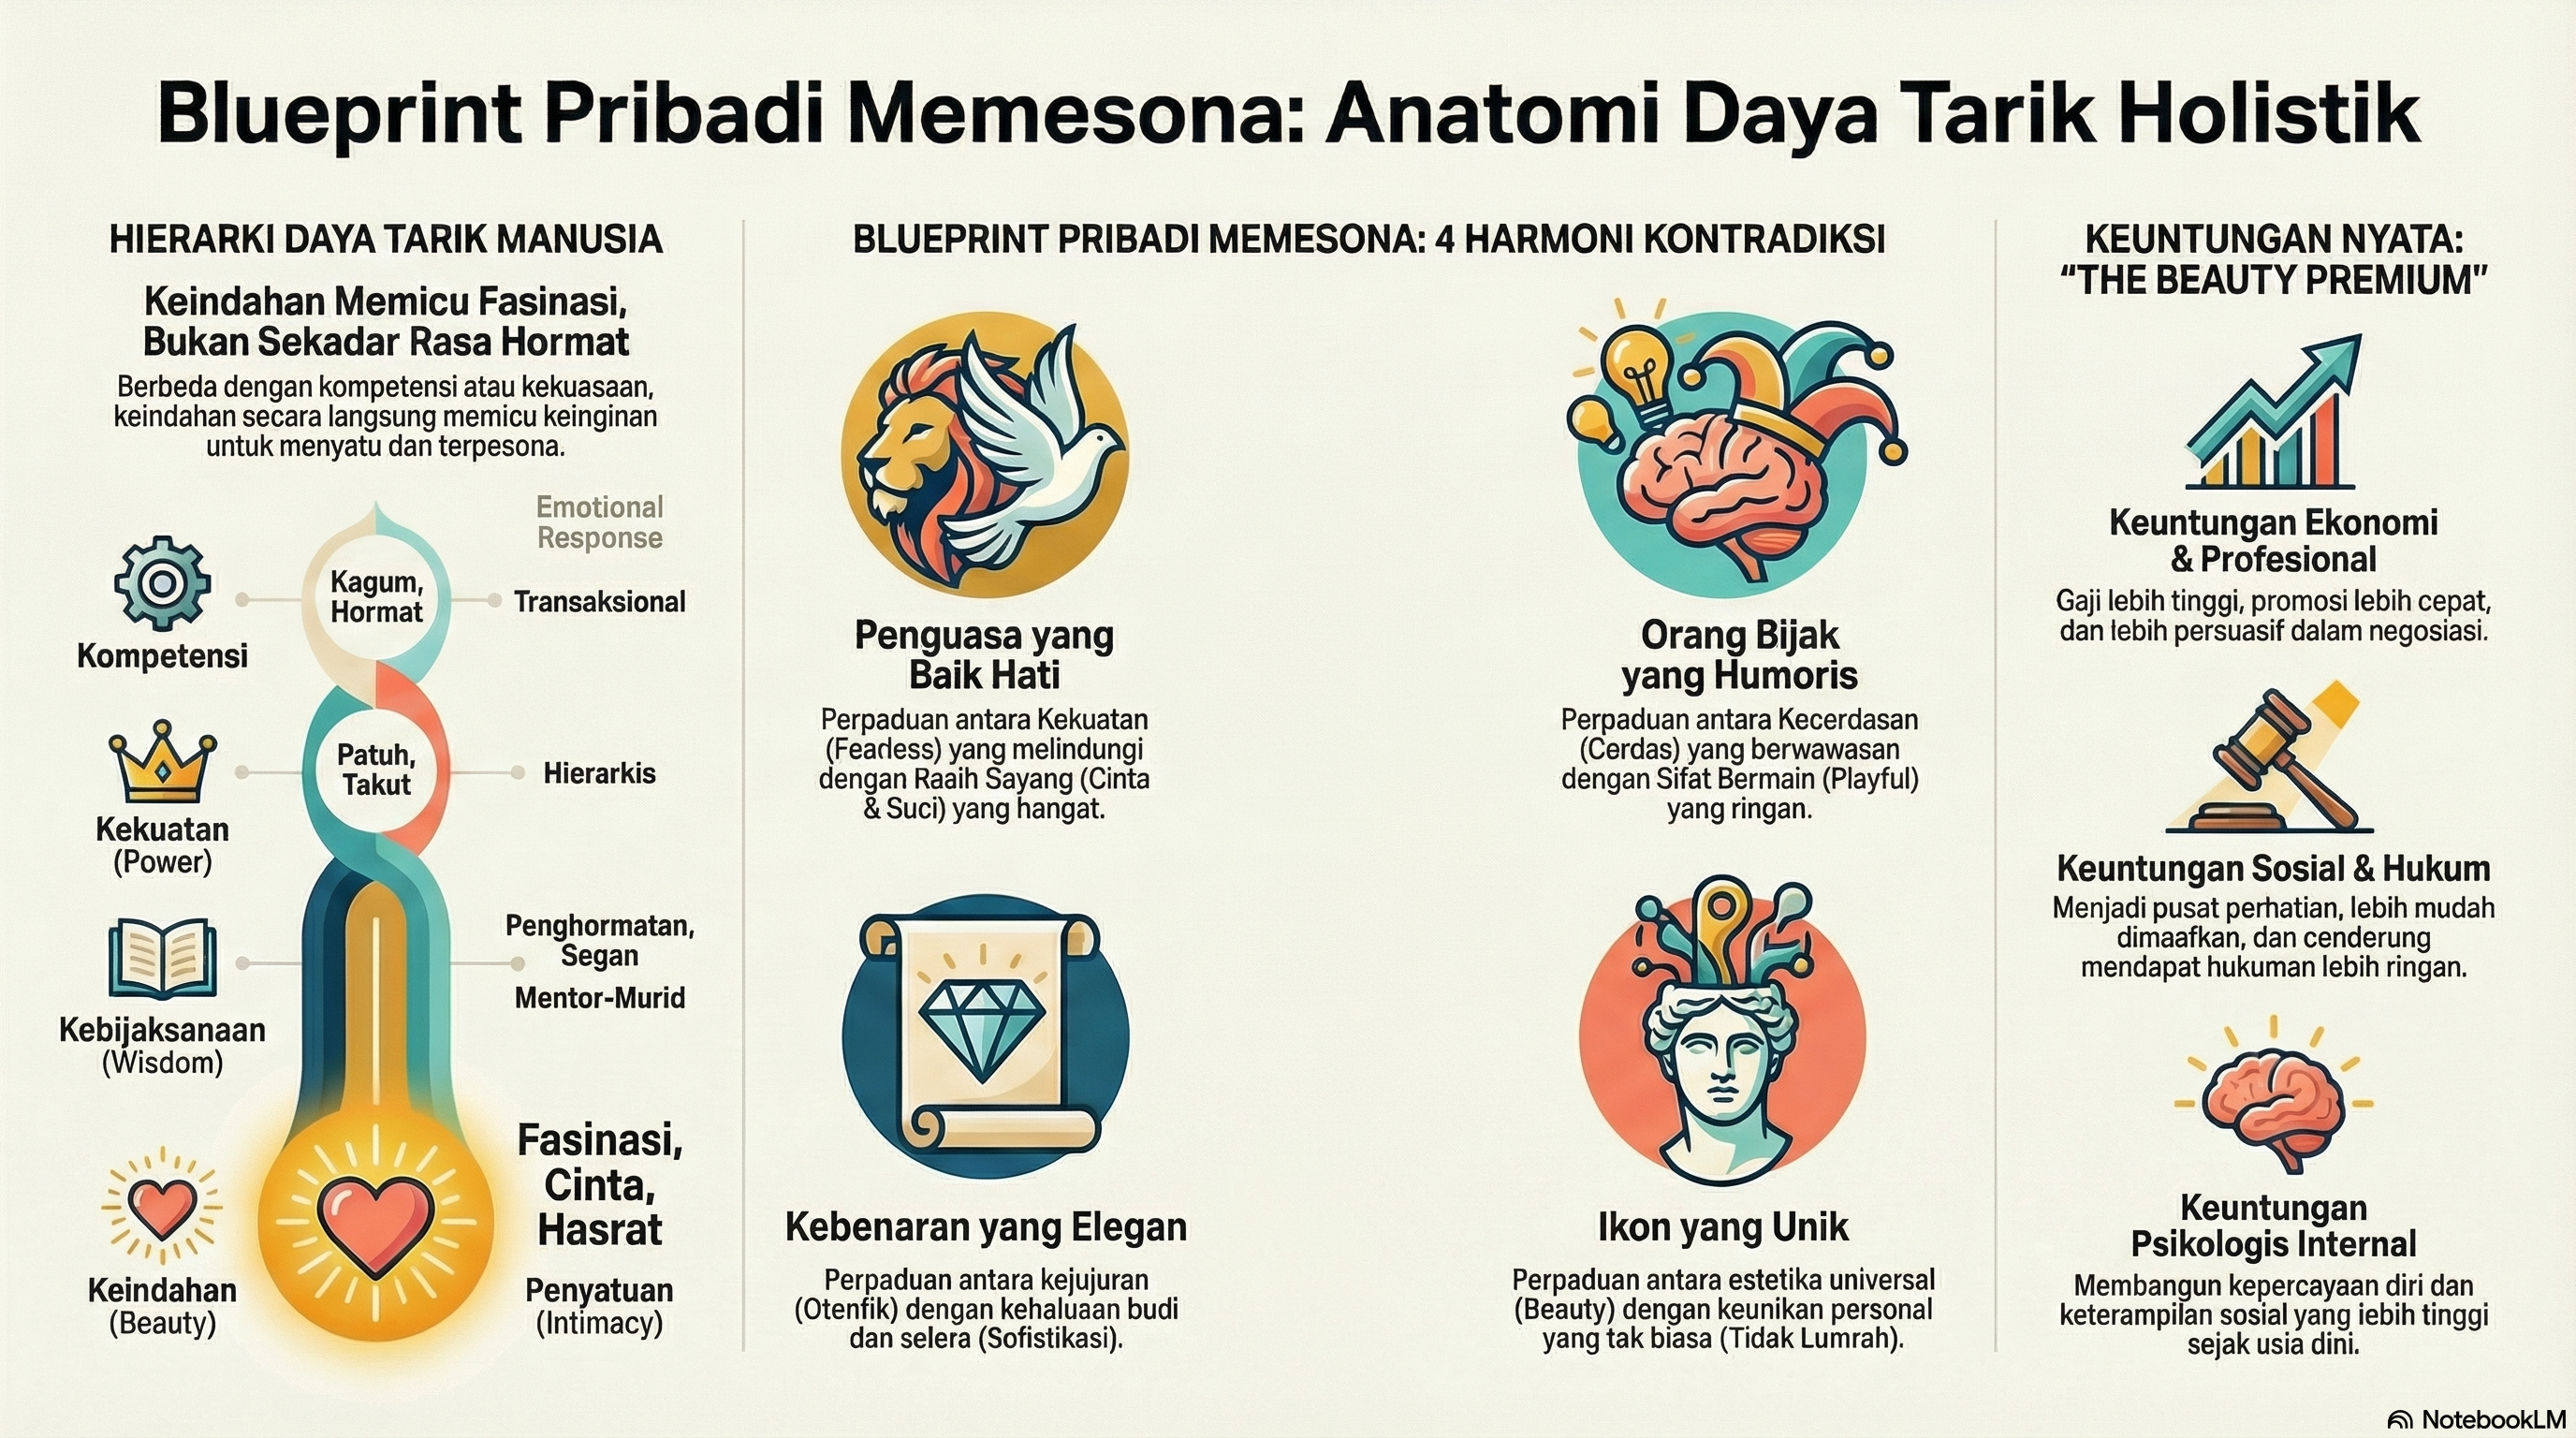
\includegraphics[keepaspectratio]{kuliah/../bahan/K-15_beauty_2.png}}

}

\caption{Beauty}

\end{figure}%

\href{https://youtube.com/playlist?list=PL_m-BplfO92F6IU_N9ZE3b8-vjDgDOHV2&si=GsLXtAtKPzTrOIe9}{Video
Clip}

Kuiz: \url{https://forms.office.com/r/5JN6rKaHHA}

\href{../bahan/K-15_Anatomi_Sang_Beautiful_Person.pdf}{Slides Pembukaan}

\href{../slides/Be\%20a\%20Beautiful\%20Person\%202024.pdf}{Slide Utama}

\href{../bahan/K15-Keindahan_Komunikasi_Diri.pdf}{Slides Pendukung}

\href{../bahan/K-13-Seni_Berpikir_Konstruktif.pdf}{Slides Interesting}

\href{../bahan/K-15-Pikiran_Yang_Indah_Seni_Meracik_Opini.pdf}{Opini}

\section{Pendahuluan: Memahami Keindahan yang
Sesungguhnya}\label{pendahuluan-memahami-keindahan-yang-sesungguhnya}

\begin{figure}[H]

{\centering \pandocbounded{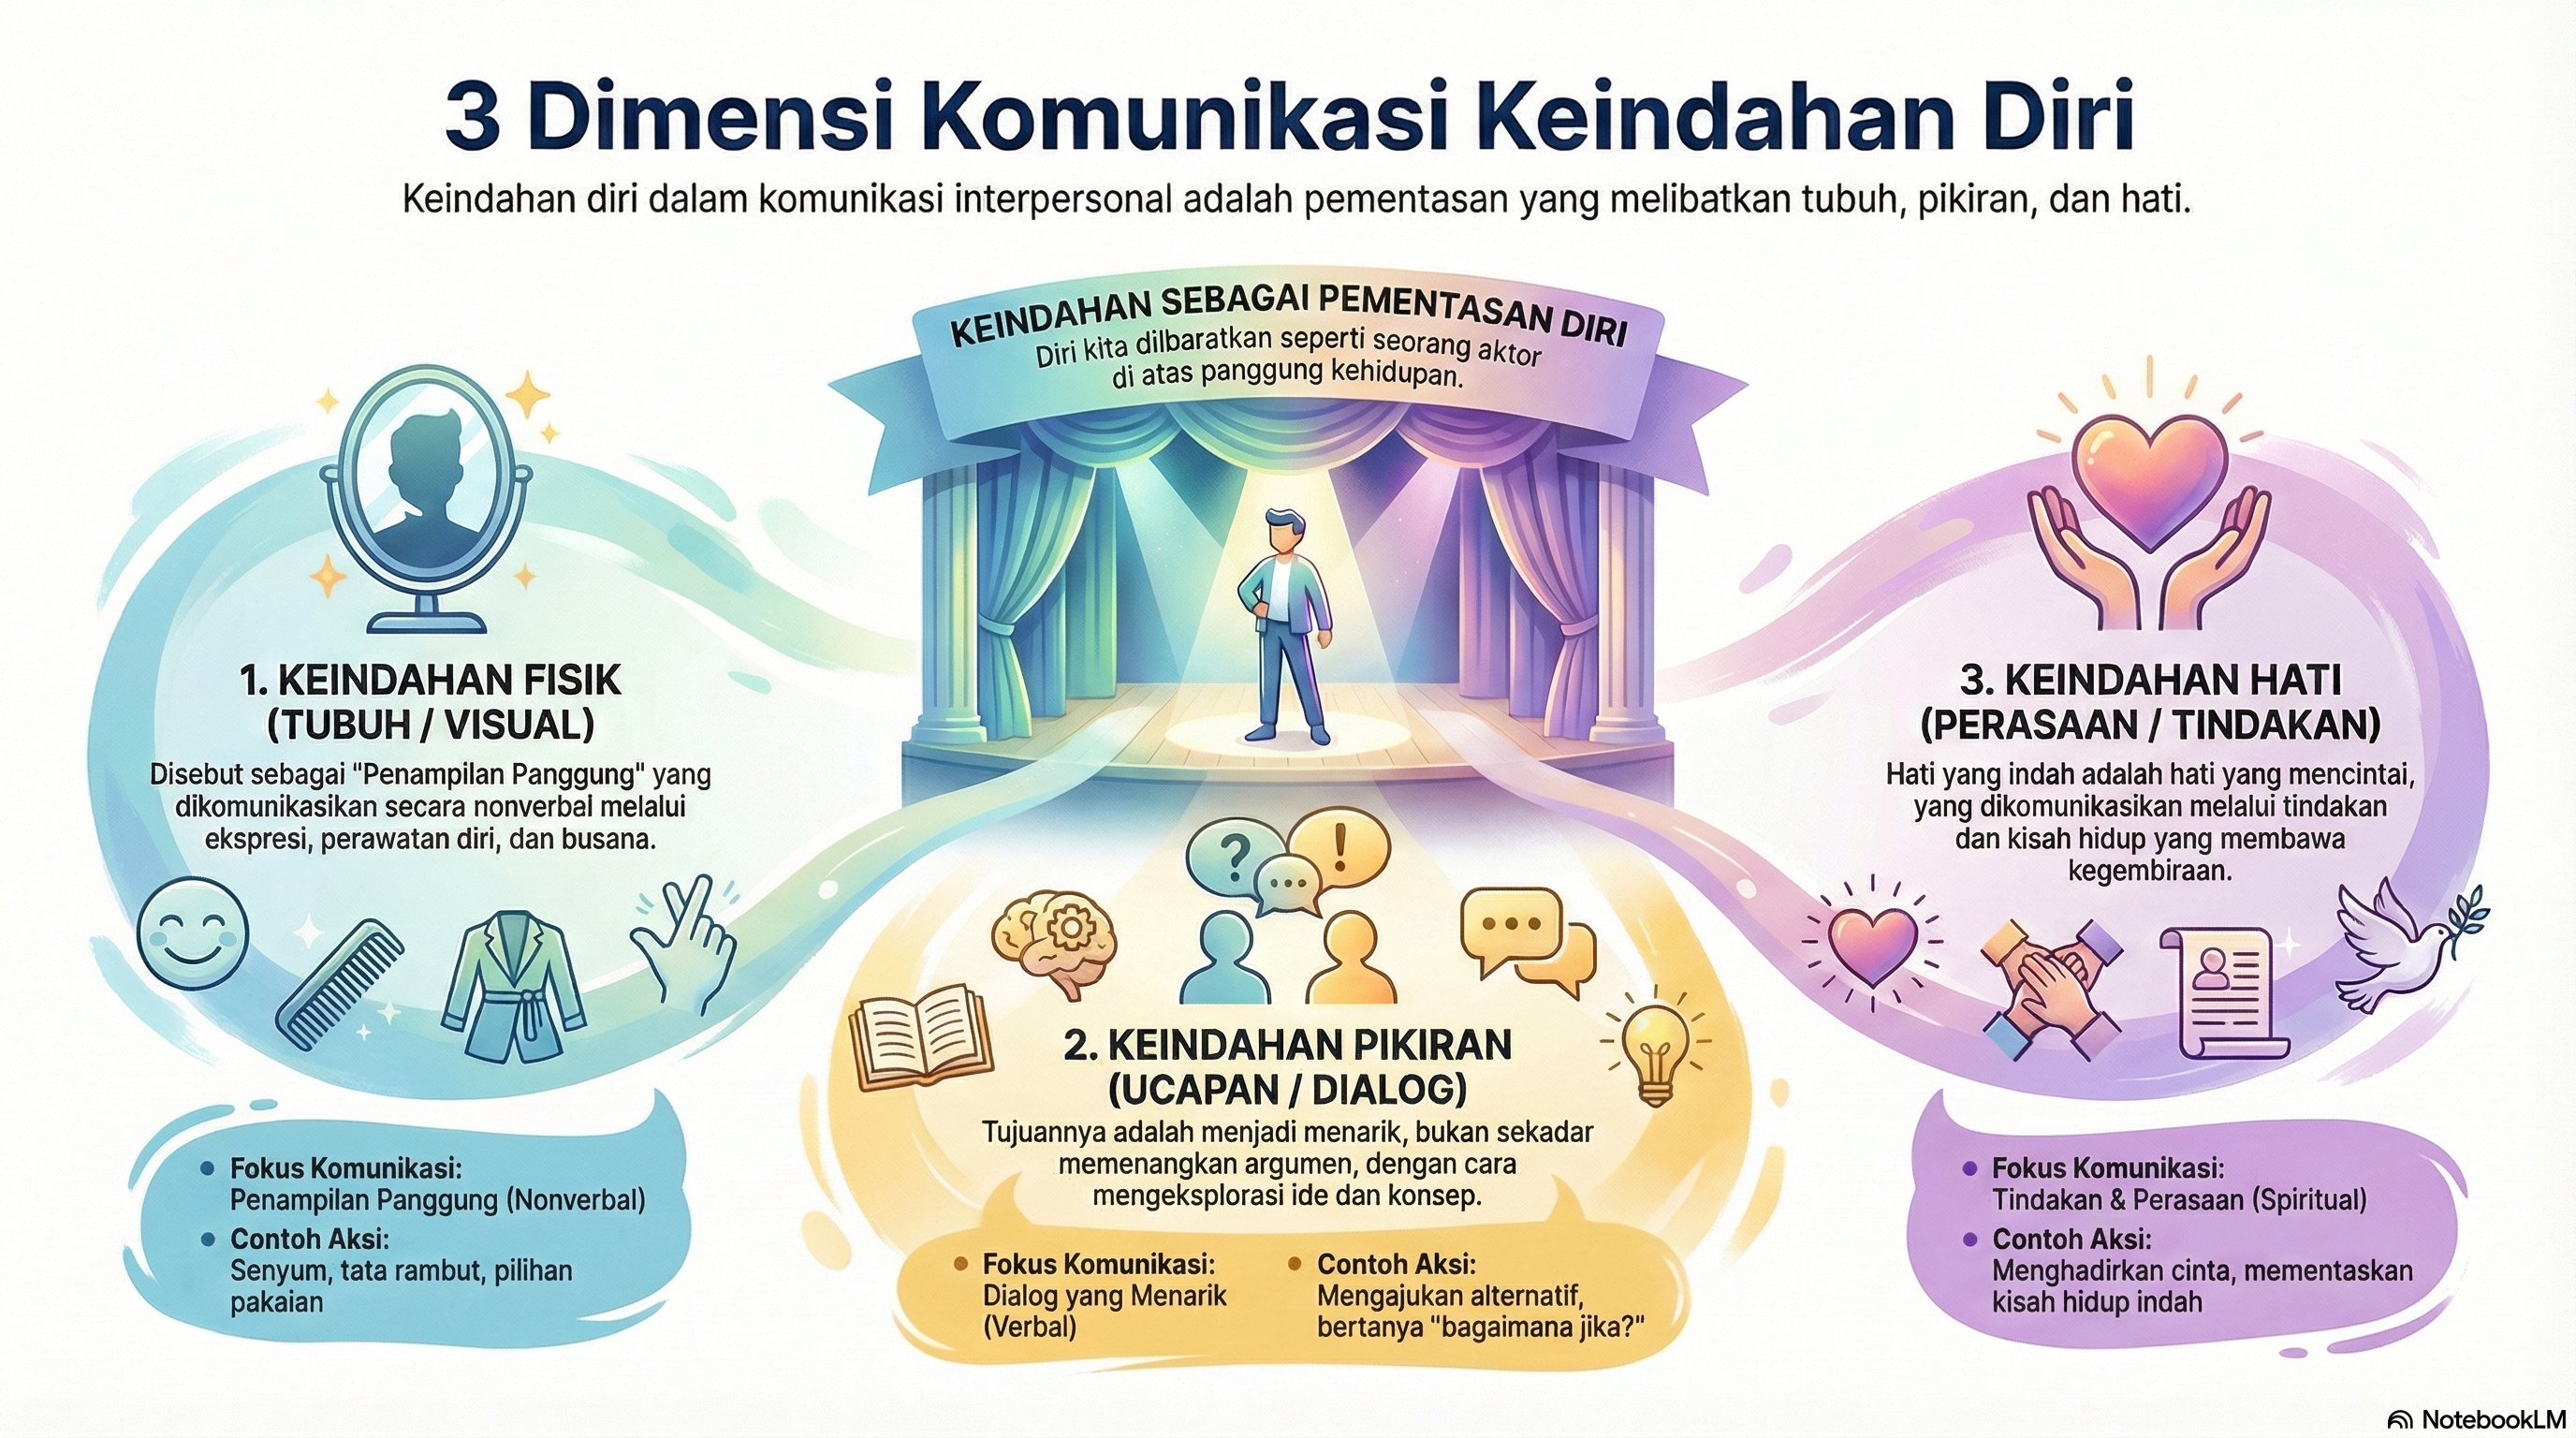
\includegraphics[keepaspectratio]{kuliah/../bahan/k-15_beauty.png}}

}

\caption{Beautiful Person}

\end{figure}%

Filsuf Confucius pernah berkata:

``Everything has beauty, but not everyone sees it.'' ― Confucius

Dari sudut pandang komunikasi, keindahan bukanlah sekadar anugerah alam,
melainkan sebuah \textbf{``Kualitas Menarik yang Dihargai Orang Lain''}
(\emph{An Attractive Quality Appreciated by Others}). Ini berarti
keindahan bukanlah takdir, melainkan sebuah pesan yang kita
kirimkan---sebuah getaran yang kita pancarkan dan dapat dirasakan oleh
setiap orang di sekitar kita.

Layaknya seorang aktor di atas panggung, cara kita menampilkan diri,
berbicara, dan membawa perasaan adalah sebuah isu komunikasi. Untuk
dapat mengkomunikasikan keindahan diri secara utuh, kita perlu menguasai
tiga dimensi utamanya: \textbf{Tubuh (Visual)}, \textbf{Pikiran
(Ucapan)}, dan \textbf{Hati (Perasaan)}.

\begin{center}\rule{0.5\linewidth}{0.5pt}\end{center}

\section{1. Dimensi Pertama: Keindahan Tubuh (Visual) - Panggung
Anda}\label{dimensi-pertama-keindahan-tubuh-visual---panggung-anda}

\subsection{Penampilan Panggung}\label{penampilan-panggung}

Dimensi pertama dari keindahan adalah apa yang terlihat oleh mata. Ini
adalah panggung kita, tempat kita menampilkan diri melalui komunikasi
non-verbal. Setiap elemen visual yang kita tampilkan mengirimkan pesan
kepada orang lain sebelum kita sempat mengucapkan sepatah kata pun.

Elemen-elemen kunci dari keindahan visual meliputi:

\begin{itemize}
\item
  \textbf{Ekspresi Wajah, Tatapan Mata, \& Gerak Tubuh} Senyum yang
  tulus, tatapan mata yang hangat, serta postur dan gerak tubuh yang
  percaya diri adalah alat komunikasi paling kuat. Ketiganya dapat
  membangun koneksi, menunjukkan keterbukaan, dan memancarkan energi
  positif secara instan.
\item
  \textbf{Perawatan Diri} Ini mencakup kebersihan diri, kesehatan
  tekstur kulit, dan tata rambut. Merawat diri menunjukkan bahwa kita
  menghargai diri sendiri, yang pada gilirannya membuat orang lain lebih
  mudah untuk menghargai kita.
\item
  \textbf{Gaya Personal} Cara kita berdandan, memilih wewangian,
  pakaian, sepatu, hingga aksesoris adalah bentuk ekspresi diri. Gaya
  personal yang terawat dan sesuai dengan karakter kita
  mengkomunikasikan identitas dan kepercayaan diri.
\end{itemize}

Meskipun beberapa aspek fisik adalah pemberian alam, sebagian besar
dapat dikembangkan melalui usaha sadar seperti menjaga pola makan,
berolahraga, dan merawat diri. Artinya, setiap orang memiliki kendali
untuk menampilkan panggung visual terbaik versi mereka.

Namun, penampilan visual hanyalah babak pembuka; dialog yang kita
bawakanlah yang akan memikat penonton.

\begin{center}\rule{0.5\linewidth}{0.5pt}\end{center}

\section{2. Dimensi Kedua: Keindahan Pikiran (Ucapan) - Dialog
Anda}\label{dimensi-kedua-keindahan-pikiran-ucapan---dialog-anda}

\begin{figure}[H]

{\centering \pandocbounded{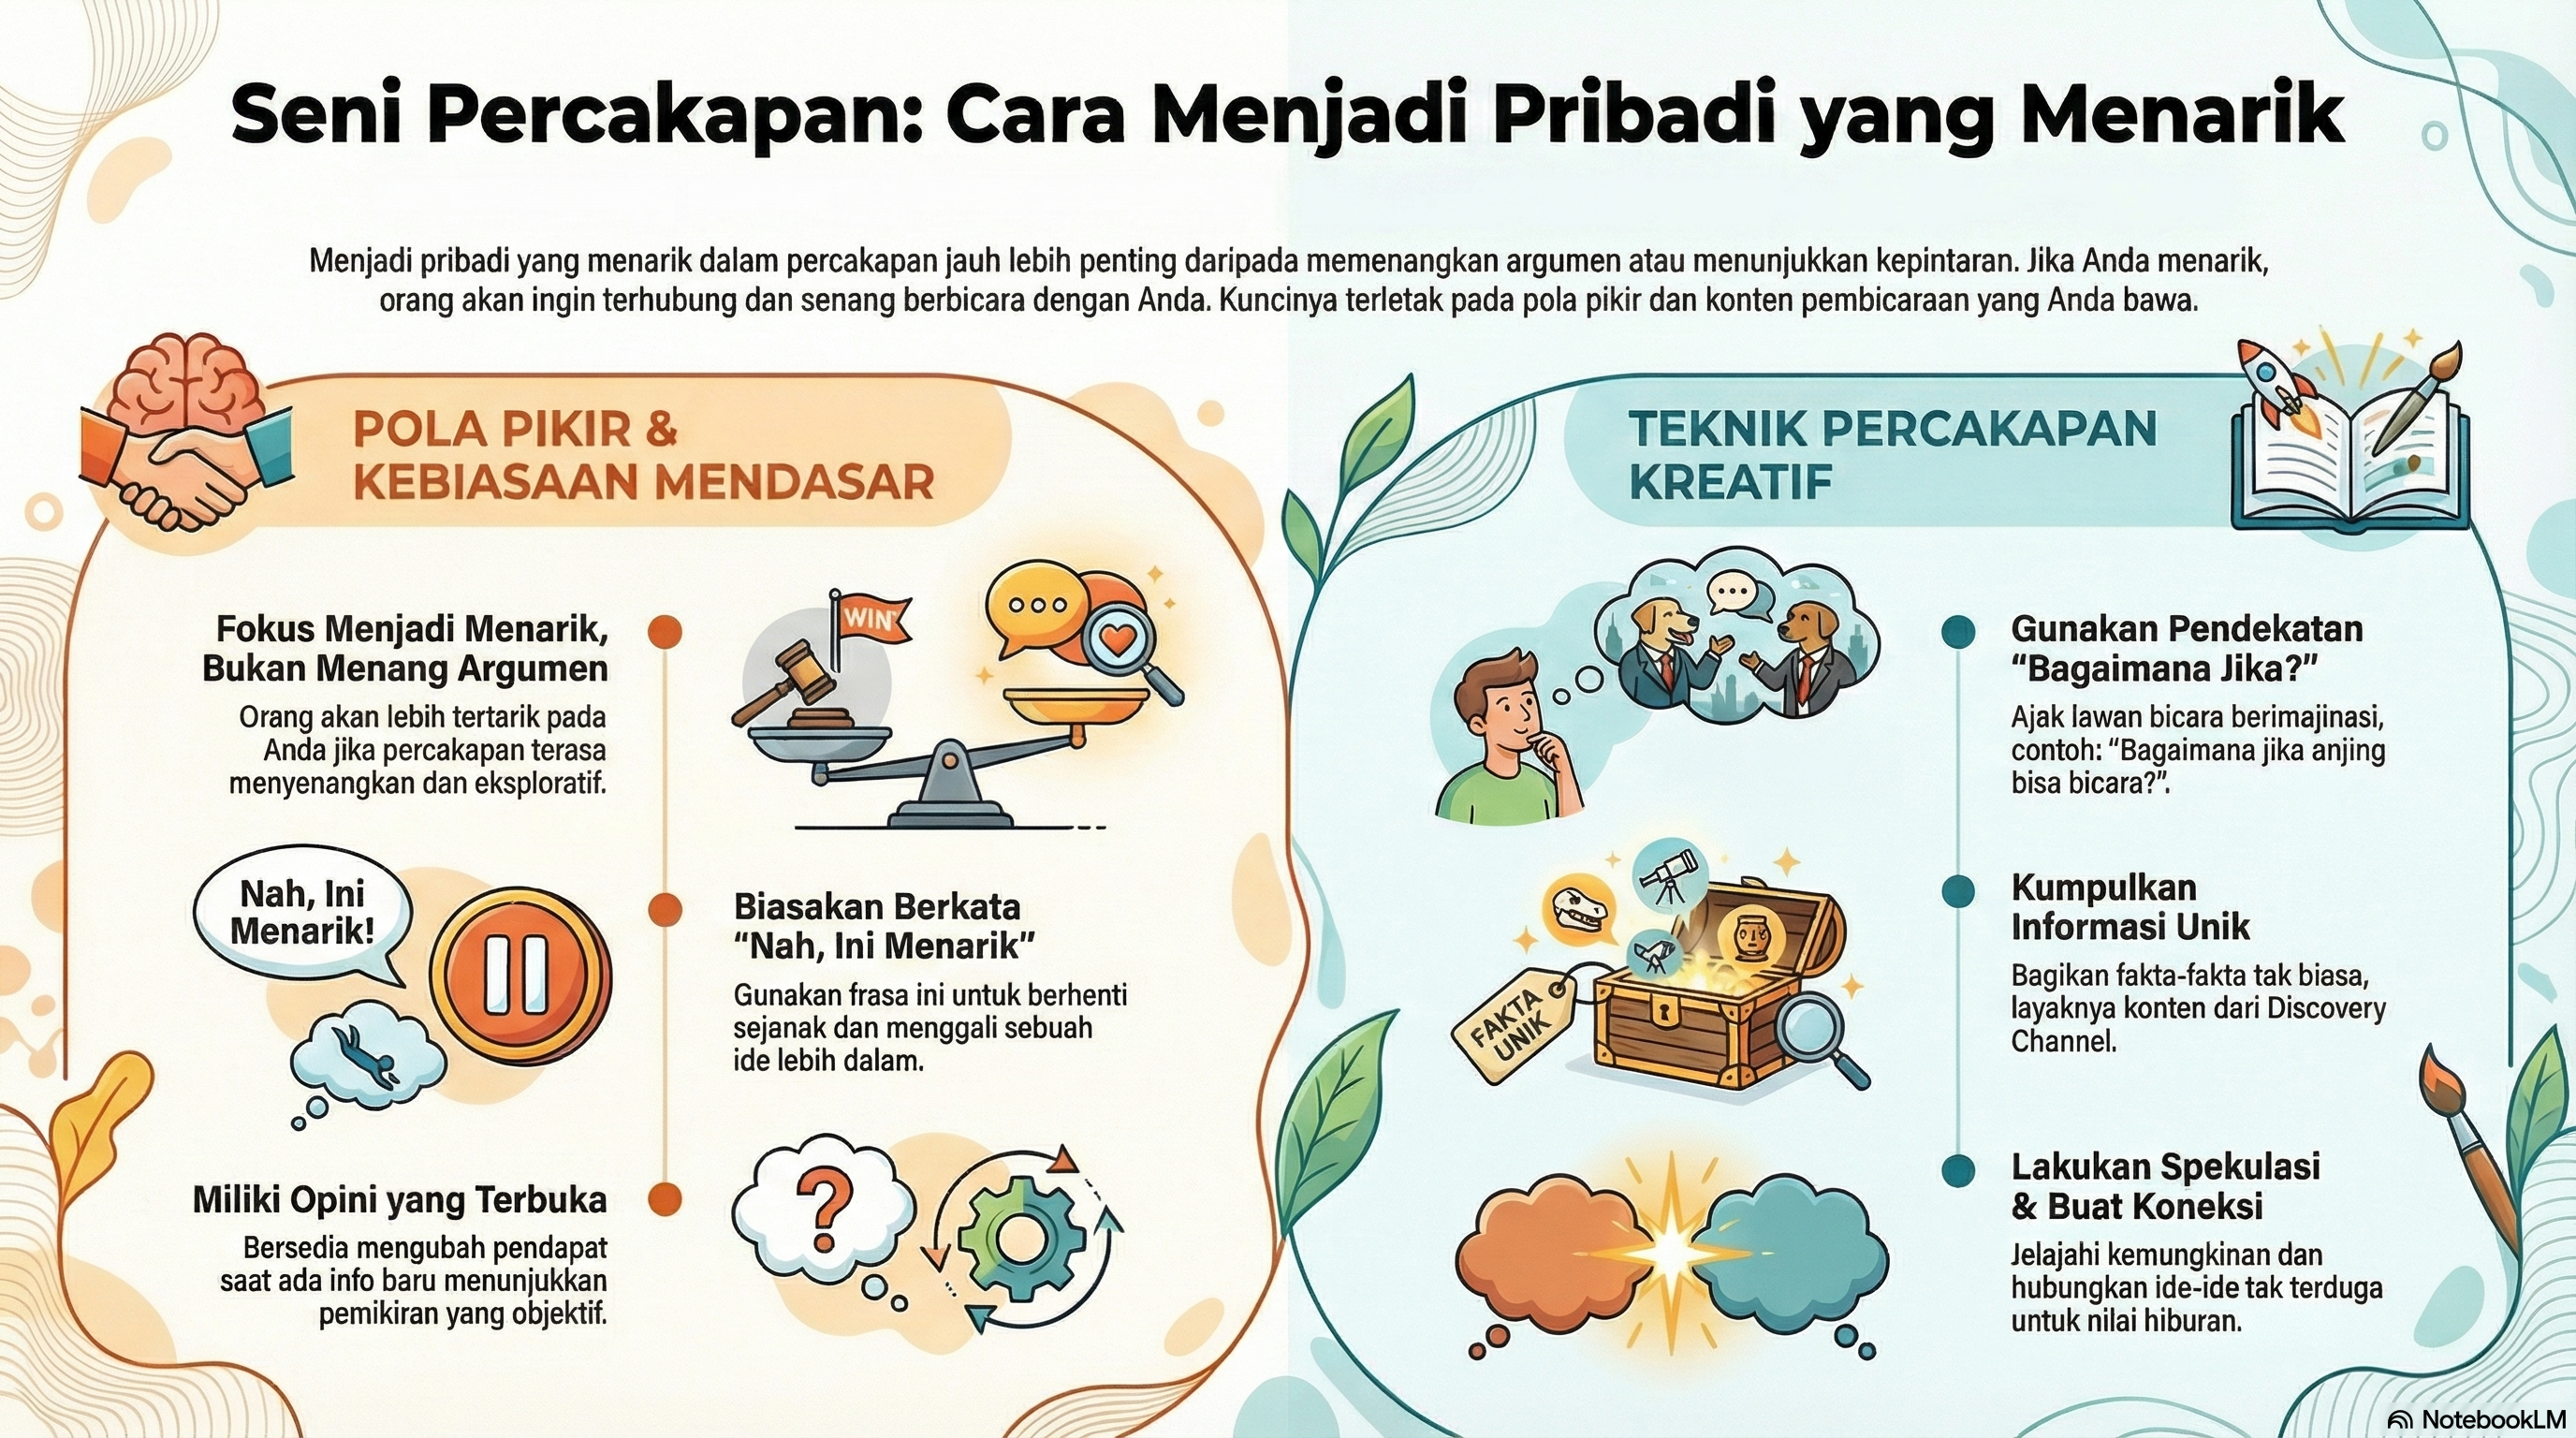
\includegraphics[keepaspectratio]{kuliah/../bahan/K-15_interesting.png}}

}

\caption{Seni dialog}

\end{figure}%

Keindahan pikiran tidak terlihat, tetapi terdengar dan terasa melalui
``Dialog''---cara kita berpikir, berbicara, dan merespons. Inilah naskah
yang menentukan kedalaman karakter yang kita perankan.

\subsection{2.1. Seni Berdialog}\label{seni-berdialog}

Berkomunikasi dengan indah adalah sebuah seni yang berpusat pada satu
filosofi: menciptakan ruang percakapan yang nyaman bagi orang lain.
Berikut adalah fondasi untuk membangun dialog yang memikat:

\begin{itemize}
\item
  \textbf{Cara Mendengar \& Bertanya} Ini adalah dasar dari semua
  koneksi yang bermakna. Mendengar dengan empati dan mengajukan
  pertanyaan yang relevan menunjukkan bahwa kita menghargai lawan bicara
  dan tulus ingin memahami mereka.
\item
  \textbf{Cara Menarik Minat (\emph{Interesting})} Orang yang indah
  secara intelektual mampu membuat topik yang sederhana sekalipun
  menjadi menarik. Bagaimana Anda bisa membuat topik seperti `kodok',
  `bandara', atau `telur dadar' menjadi percakapan yang menarik? Inilah
  letak keindahan pikiran---kemampuan untuk melihat dan
  mengkomunikasikan hal-hal yang tidak biasa dari yang biasa.
\item
  \textbf{Cara Setuju, Tidak Setuju, \& Berbeda} Keindahan dialog bukan
  hanya tentang selalu setuju. Kemampuan menyampaikan persetujuan dengan
  antusias, dan ketidaksetujuan dengan hormat menunjukkan kematangan
  berpikir. Lebih dari itu, seni ini juga tentang mengetahui kapan harus
  menawarkan ``cara berbeda''---sebuah perspektif alternatif tanpa
  konfrontasi langsung---yang menunjukkan integritas intelektual dan
  rasa hormat.
\item
  \textbf{Cara Menjawab} Memberikan jawaban yang bernas, penuh
  pertimbangan, dan tidak terburu-buru adalah cerminan dari pikiran yang
  jernih dan terstruktur.
\end{itemize}

\subsection{2.2. Kerangka Berpikir yang Indah: Enam Topi
Bono}\label{kerangka-berpikir-yang-indah-enam-topi-bono}

Di balik dialog yang indah, terdapat kerangka berpikir yang terstruktur.
Kerangka ini memungkinkan kita untuk mendekati percakapan dengan
fleksibilitas dan kedalaman, memastikan kita tidak terjebak dalam satu
cara berpikir saja, tetapi mampu menavigasi sebuah diskusi secara
holistik. Metode ``Enam Topi Berpikir'' dari Edward de Bono menawarkan
kerangka kerja yang kuat untuk tujuan ini.

\begin{longtable}[]{@{}
  >{\raggedright\arraybackslash}p{(\linewidth - 4\tabcolsep) * \real{0.3333}}
  >{\raggedright\arraybackslash}p{(\linewidth - 4\tabcolsep) * \real{0.3333}}
  >{\raggedright\arraybackslash}p{(\linewidth - 4\tabcolsep) * \real{0.3333}}@{}}
\toprule\noalign{}
\endhead
\bottomrule\noalign{}
\endlastfoot
Warna Topi & Fokus Utama & Manfaat dalam Percakapan \\
\textbf{Putih} & Fakta & Memastikan diskusi didasarkan pada informasi
yang objektif. \\
\textbf{Merah} & Intuisi \& Perasaan & Memberi ruang bagi emosi dan
firasat tanpa perlu pembenaran. \\
\textbf{Hitam} & Kritis \& Hati-hati & Mengidentifikasi potensi risiko
dan kelemahan dari sebuah ide. \\
\textbf{Kuning} & Optimis \& Positif & Menemukan nilai dan manfaat dari
sebuah gagasan. \\
\textbf{Hijau} & Peluang \& Kreativitas & Mendorong lahirnya ide-ide
baru dan alternatif solusi. \\
\textbf{Biru} & Review \& Proses & Mengatur alur pemikiran dan
memastikan semua perspektif telah dieksplorasi. \\
\end{longtable}

Ketika pikiran yang terstruktur bertemu dengan niat yang tulus, kita
mulai menyentuh dimensi keindahan yang paling dalam: keindahan hati.

\begin{figure}[H]

{\centering \pandocbounded{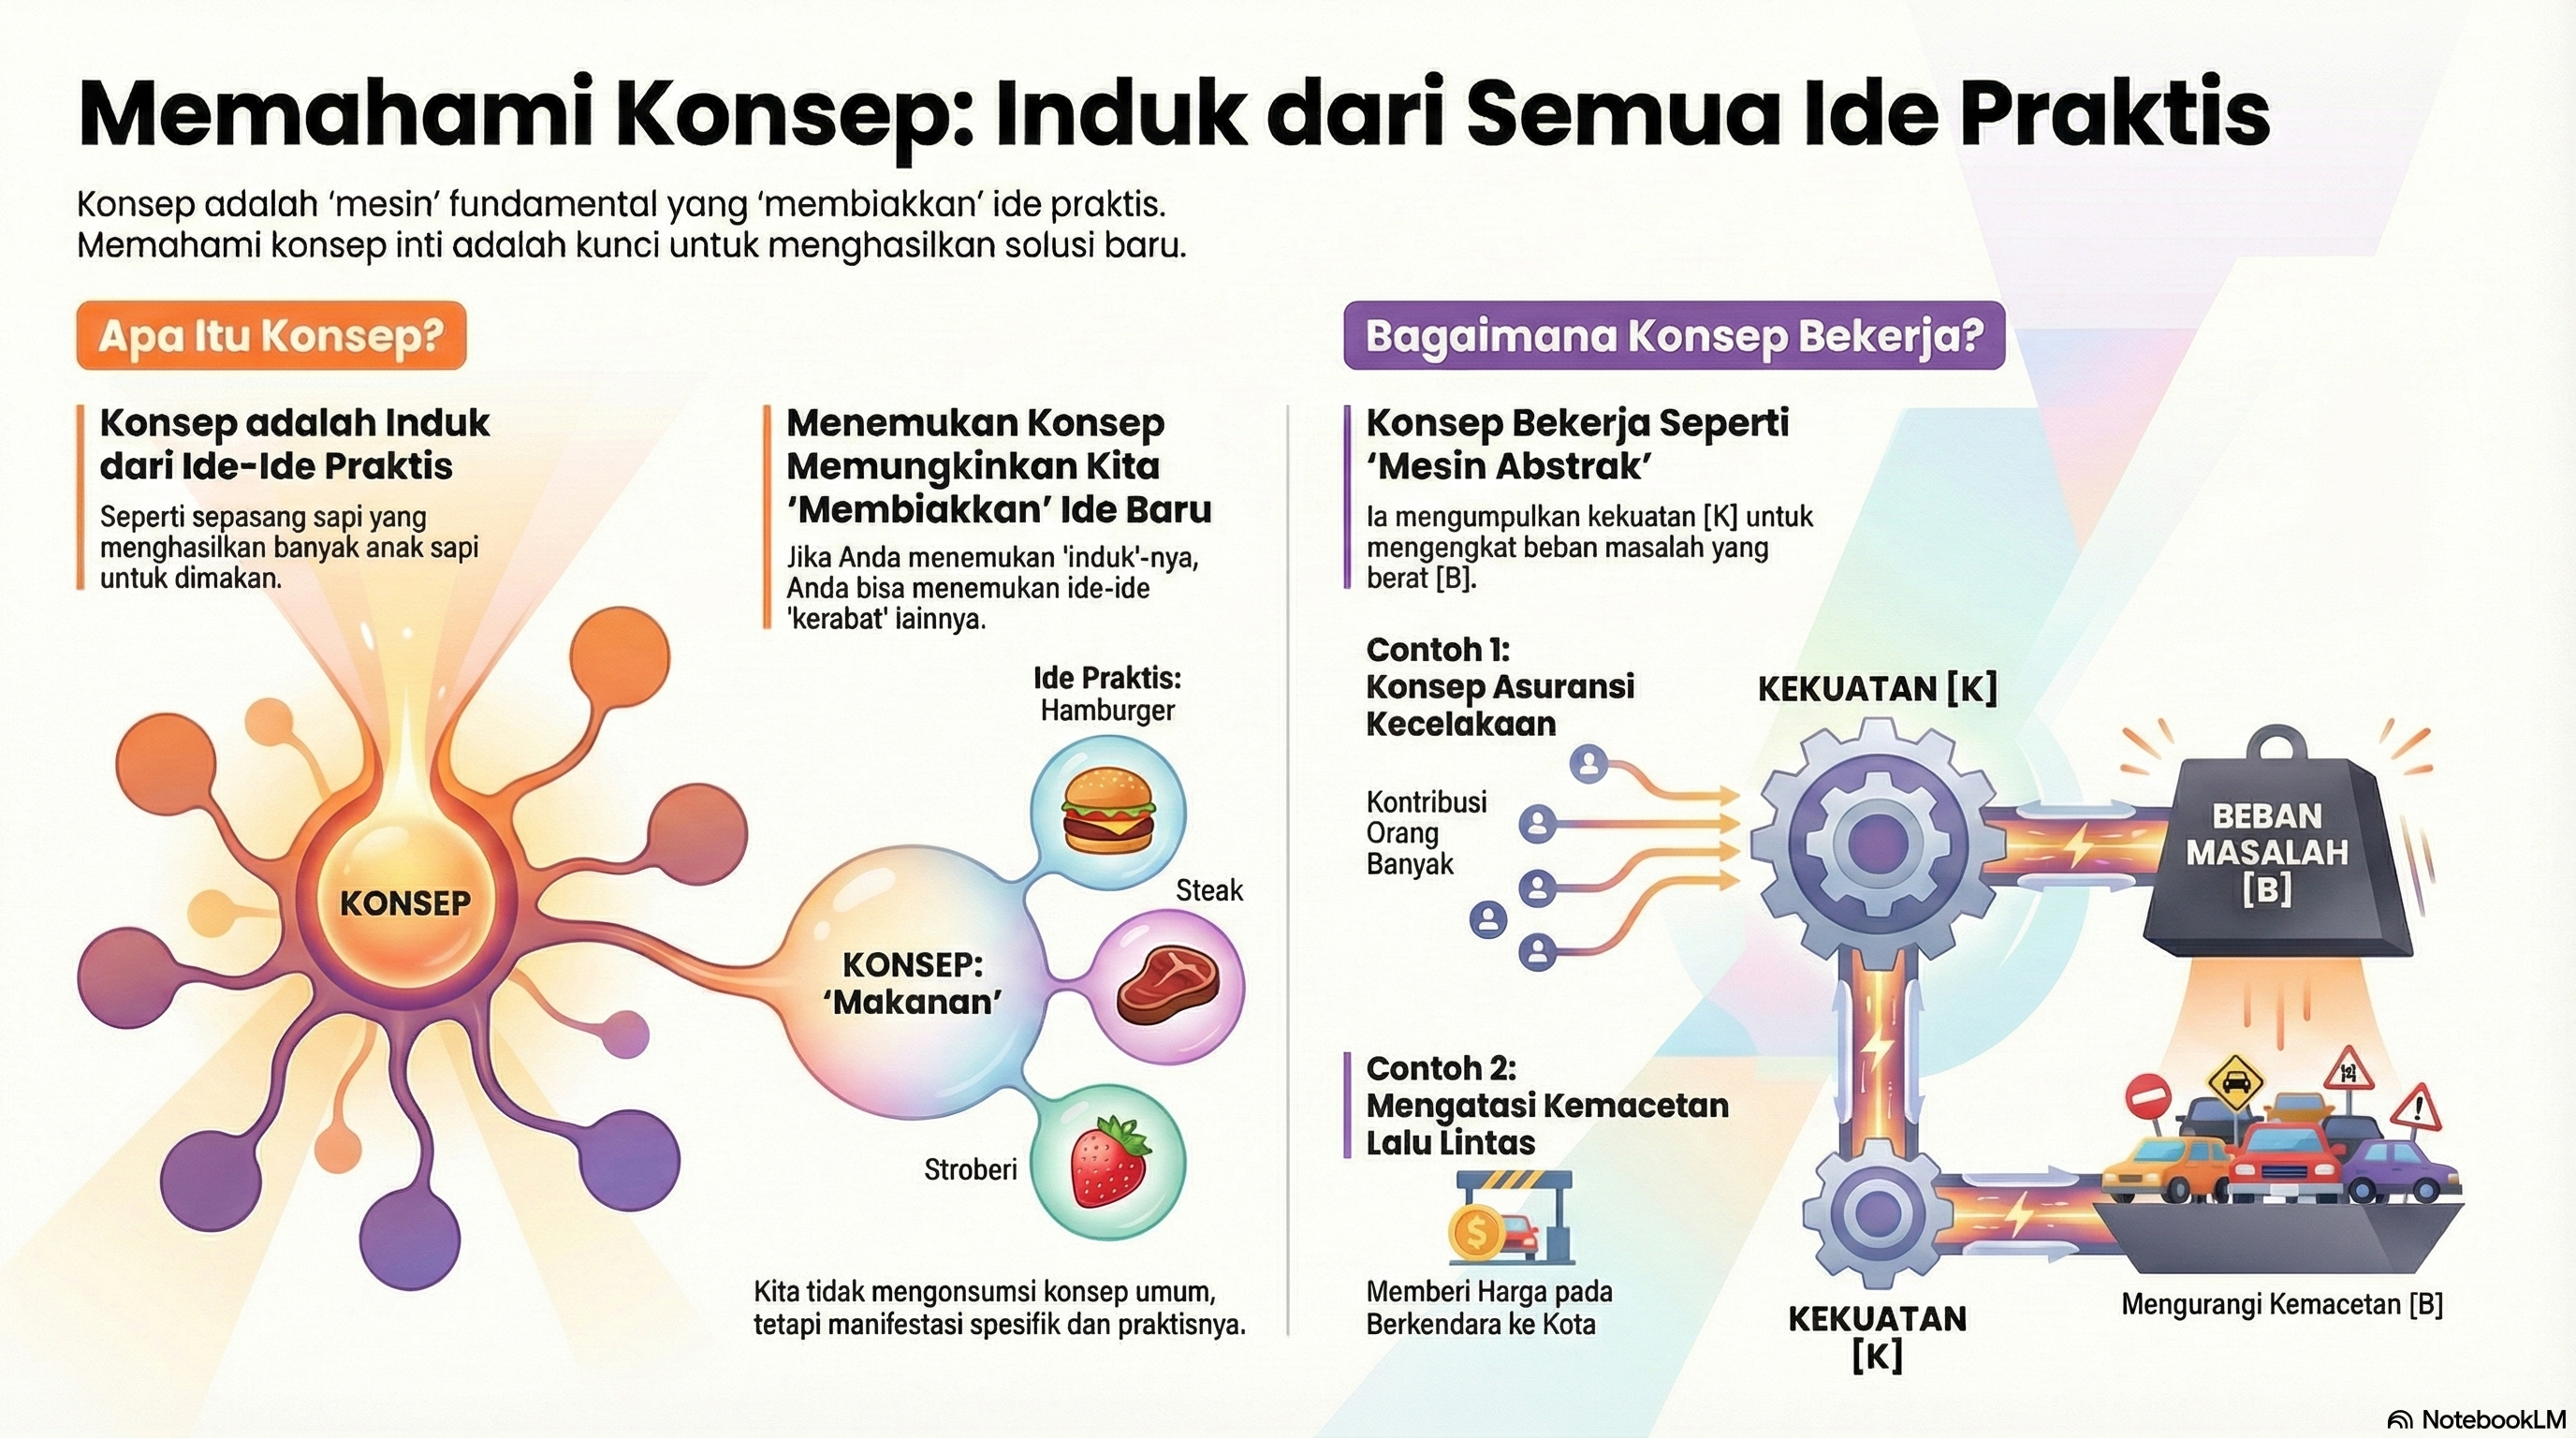
\includegraphics[keepaspectratio]{kuliah/../bahan/k-15_konsep.png}}

}

\caption{Berkonsep}

\end{figure}%

\begin{center}\rule{0.5\linewidth}{0.5pt}\end{center}

\section{3. Dimensi Ketiga: Keindahan Hati (Perasaan) - Sutradara Batin
Anda}\label{dimensi-ketiga-keindahan-hati-perasaan---sutradara-batin-anda}

Aktris legendaris Sophia Loren menangkap esensi dari dimensi keindahan
terdalam ini dengan sempurna:

``Beauty is how you feel inside, and it reflects in your eyes. It is not
something physical.''

``Nothing makes a woman more beautiful than the belief that she is
beautiful.''

Keindahan hati bersifat spiritual; ia adalah sebuah keyakinan yang
bersemayam di dalam diri. Inilah sumber dari semua keindahan lainnya.
Jika tubuh adalah panggung dan pikiran adalah dialog, maka hati adalah
sutradara yang mengarahkan keseluruhan pertunjukan.

Kita semua sedang \textbf{mementaskan autobiografi} kita setiap hari.
Hati kitalah yang menjadi sutradara. Pertanyaannya adalah: kisah hidup
seperti apa yang ingin kita pentaskan? Apakah sebuah kisah tentang
bertahan hidup semata---makan, bekerja, menua? Ataukah sebuah kisah yang
lebih agung? Hati yang indah secara sadar memilih untuk menyutradarai
sebuah mahakarya.

Pada intinya, \textbf{Hati yang Indah adalah Hati yang Mencintai}.
Tujuan dari sebuah kisah hidup yang indah adalah untuk ``menghadirkan
cinta di dunia'' dan ``membawa kegembiraan dalam kehidupan''. Inilah
pesan utama yang ingin disampaikan, karena pada akhirnya:

\textbf{Beautiful People Communicate Love.}

\begin{center}\rule{0.5\linewidth}{0.5pt}\end{center}

\section{Kesimpulan: Harmoni Tiga
Dimensi}\label{kesimpulan-harmoni-tiga-dimensi}

Keindahan sejati bukanlah entitas tunggal, melainkan sebuah harmoni dari
tiga dimensi yang saling melengkapi:

\begin{itemize}
\item
  \textbf{Tubuh} sebagai panggung visual yang kita rawat.
\item
  \textbf{Pikiran} sebagai dialog memikat yang kita bangun.
\item
  \textbf{Hati} sebagai sutradara batin yang mengarahkan semuanya dengan
  cinta.
\end{itemize}

Penting untuk dipahami bahwa komposisi keindahan ini berubah seiring
bertambahnya usia. Saat kita menua, peran penampilan visual (tubuh)
mungkin berkurang, sementara kedalaman pikiran (ucapan) dan terutama
kehangatan hati (perasaan) menjadi semakin dominan dan bernilai.

Seperti yang dikatakan Sophia Loren, keindahan dimulai dari keyakinan.
Dengan memegang kendali atas ketiga dimensi ini, Anda bukan lagi sekadar
penonton, melainkan sutradara ahli dari mahakarya terindah Anda: diri
Anda sendiri.

\bookmarksetup{startatroot}

\chapter{Materi UAS}\label{materi-uas}

Tugas kita adalah membuat

\section{Konsep}\label{konsep}

Konsep adalah bagian yang sangat penting dalam berpikir. Jika Anda ingin
memiliki \textbf{pikiran yang indah}, Anda harus mampu menangani konsep.

Menurut sumber, konsep didefinisikan dan dijelaskan sebagai berikut:

\subsection{Definisi dan Esensi
Konsep}\label{definisi-dan-esensi-konsep}

\begin{itemize}
\tightlist
\item
  \textbf{KONSEP adalah logika mesin abstrak}, yang bekerja untuk
  mengumpulkan dan mengarahkan kekuatan yang ada \textbf{{[}K{]}} guna
  mengangkat beban masalah yang berat \textbf{{[}B{]}}.
\item
  Konsep dapat dilihat sebagai \textbf{singkatan, ringkasan, atau esensi
  mendasar} dari apa yang dikatakan.
\item
  Konsep berusaha untuk \textbf{menyaring esensi} dari apa yang sedang
  dipikirkan atau dilakukan. Meskipun konsep, definisi, dan deskripsi
  tumpang tindih, deskripsi harus lengkap, sedangkan konsep berupaya
  menyaring esensi.
\item
  Konsep tidak selalu lengkap, tetapi mereka membawa \textbf{aspek-aspek
  penting} dari apa yang sedang dipikirkan atau dilakukan.
\item
  Kebanyakan orang menganggap `konsep' itu kabur, abstrak, dan akademis.
  Namun, konsep akan selalu tampak samar karena memang harus
  diterjemahkan ke dalam ide-ide tertentu sebelum dapat digunakan.
\item
  Sama seperti mesin, logika mesin abstrak (konsep) bisa kuat, lemah,
  atau bahkan hanya angan-angan (\emph{wishful thinking}).
\end{itemize}

\subsection{Peran dan Pentingnya
Konsep}\label{peran-dan-pentingnya-konsep}

Konsep memiliki peran sentral dalam proses berpikir, bertindak sebagai
fondasi untuk ide-ide praktis:

\begin{enumerate}
\def\labelenumi{\arabic{enumi}.}
\tightlist
\item
  \textbf{Induk dari Ide Praktis:} Konsep adalah \textbf{induk dari
  ide-ide praktis}. Setelah konsep dibuat (yang memerlukan kerja keras),
  ia dapat menghasilkan turunan buah pikiran praktis yang memiliki
  kualitas seperti induknya.
\item
  \textbf{Membiakkan Ide:} Nilai utama dalam mengidentifikasi konsep
  adalah hal ini memungkinkan kita untuk \textbf{`membiakkan' ide-ide
  lain} dari konsep tersebut. Konsep seperti orang tua yang membiakkan
  anak-anak (ide).
\item
  \textbf{Arah dan Jalan Baru:} Konsep dapat dipandang sebagai
  persimpangan jalan yang membuka beberapa jalan lain. Konsep sangat
  penting dalam menghasilkan ide dan merancang cara ke depan, terutama
  di mana tidak ada rutinitas yang tersedia.
\item
  \textbf{Komponen Kunci Pikiran:} Konsep adalah komponen kunci dari
  pikiran yang indah (\emph{beautiful mind}).
\end{enumerate}

\subsection{Penerapan Konsep dalam Kehidupan
Sehari-hari}\label{penerapan-konsep-dalam-kehidupan-sehari-hari}

Anda perlu berusaha untuk memilih konsep di balik apa yang dikatakan
atau dibaca. Setelah Anda dapat memilih konsep, Anda dapat membandingkan
dan mengontraskannya untuk melihat apakah mereka benar-benar berbeda dan
apa saja poin perbedaannya.

\textbf{Contoh Konsep:}

\begin{itemize}
\tightlist
\item
  \textbf{Makanan (Konsep) dan Hamburger (Ide Praktis):} Anda selalu
  makan `makanan', tetapi Anda sebenarnya makan jenis makanan tertentu
  (steak, ayam, stroberi). Makanan adalah sebuah konsep, sedangkan
  hamburger adalah ide praktisnya.
\item
  \textbf{Asuransi Kecelakaan:} Konsepnya mungkin adalah
  \textbf{mengumpulkan semua orang yang terkena risiko {[}K{]}} untuk
  berkontribusi pada mereka yang benar-benar menderita akibat kecelakaan
  tersebut {[}B{]}.
\item
  \textbf{Hewan Peliharaan:} Konsepnya dapat didefinisikan sebagai
  \textbf{makhluk hidup {[}K{]}} yang dipelihara di rumah dengan tujuan
  utama untuk dicintai (termasuk persahabatan) \textbf{{[}B{]}}.
\item
  \textbf{Maksimalisasi Tempat Parkir:} Konsep pengoperasian yang
  ditetapkan untuk mengatasi kemacetan di perkotaan, yaitu `memberi
  harga pada berkendara ke dalam kota', dapat dilakukan dengan berbagai
  cara, seperti melalui sistem izin khusus atau lelang.
\end{itemize}

Ada berbagai jenis konsep, seperti konsep bisnis, konsep nilai, konsep
mekanisme, dan konsep operasi. Di mana pun ada ide, di sana juga ada
konsep. Untuk menghasilkan konsep, kita perlu cara untuk melihat
bagaimana sesuatu beroperasi menggunakan kekuatan yang dihimpun untuk
mengangkat beban persoalan yang berat. Salah satu cara yang efisien
untuk menghasilkan konsep baru adalah dengan meminjam konsep-konsep yang
sudah ada untuk `membiakkan' konsep baru. Keterampilan dalam berpikir
dalam hal konsep hanya datang dengan praktik.

\begin{center}\rule{0.5\linewidth}{0.5pt}\end{center}

\textbf{Analogi untuk Memperjelas:} Jika ide-ide praktis adalah ``buah''
yang kita petik dan nikmati, maka \textbf{konsep} adalah ``induk pohon''
yang harus dibangun dan dipelihara. Meskipun pohon (konsep) mungkin
terlihat abstrak, ia adalah sumber berkelanjutan yang memungkinkan kita
membiakkan buah-buah (ide-ide) baru tanpa harus mengulangi seluruh
proses dari awal setiap kali kita ingin makan.

\section{OPINI}\label{opini}

Opini atau pendapat adalah elemen penting yang dibahas dalam konteks
memiliki pikiran yang indah (\emph{beautiful mind}), dan didefinisikan
secara komprehensif oleh sumber Anda.

Berikut adalah penjelasan mengenai apa yang dimaksud dengan opini:

\subsection{Definisi dan Komponen
Opini}\label{definisi-dan-komponen-opini}

Opini (pendapat) didefinisikan sebagai \textbf{semacam rebusan} yang
terdiri dari \textbf{informasi, persepsi, perasaan, dan nilai-nilai},
yang semuanya dimasak bersama dalam budaya tertentu.

Pendapat muncul dari kombinasi hal-hal berikut: 1. \textbf{Informasi} 2.
\textbf{Nilai-nilai} 3. \textbf{Perasaan} 4. \textbf{Pengalaman}

Semua komponen ini disatukan dalam \textbf{budaya lokal}.

\subsection{Sifat dan Sudut Pandang
Opini}\label{sifat-dan-sudut-pandang-opini}

\begin{itemize}
\tightlist
\item
  \textbf{Sudut Pandang:} Pendapat didasarkan pada \textbf{sudut
  pandang} yang merupakan serangkaian keadaan di mana Anda ditempatkan.
\item
  \textbf{Jenis Opini:} Anda dapat memilih untuk mengajukan pendapat
  berdasarkan \textbf{sudut pandang Anda yang sangat pribadi}, atau
  pendapat tentang apa yang mungkin terbaik \textbf{`secara umum'} atau
  untuk semua orang.
\item
  Penting untuk memberi sinyal sifat pendapat yang Anda ajukan, apakah
  itu pribadi atau lebih umum.
\item
  Terdapat dua ekstrem dalam memiliki pendapat: \textbf{memiliki
  pendapat yang kuat yang didasarkan pada sangat sedikit} informasi,
  atau \textbf{menolak memiliki pendapat ketika Anda diberitahu dengan
  baik} (diberi informasi yang memadai). Yang terbaik adalah berada di
  antara kedua ekstrem ini.
\end{itemize}

\subsection{Opini dan Pikiran yang
Indah}\label{opini-dan-pikiran-yang-indah}

Salah satu karakteristik penting dari pikiran yang indah adalah kesiapan
untuk mengubah pendapat.

Pendapat dapat diubah melalui beberapa cara: 1. Melalui
\textbf{informasi baru}. 2. Melalui \textbf{penerimaan nilai-nilai
lain}. 3. Pendapat dapat dikurangi dari generalisasi yang luas ke bentuk
yang kurang lengkap.

\subsection{Menangani Perbedaan Opini}\label{menangani-perbedaan-opini}

Ketika menghadapi pendapat yang berbeda, tujuannya adalah: 1.
\textbf{Meletakkan pendapat yang berbeda berdampingan} satu sama lain.
2. Melakukan upaya untuk \textbf{menjelajahi dasar perbedaan} tersebut.
3. Berusaha untuk memengaruhi rekonsiliasi. Jika rekonsiliasi tidak
mungkin, setidaknya ada kesepakatan untuk berbeda.

\subsection{Opini dan Sikap}\label{opini-dan-sikap}

Meskipun opini adalah produk dari pemikiran, beberapa sikap
(\emph{attitude}) dapat memengaruhi cara orang menyampaikan atau
membentuk pendapat mereka, misalnya: * Orang `pintar' yang harus benar
dan lebih pintar dari orang lain. * `Wali nilai' (\emph{value
guardians}) yang bersikeras bahwa hanya nilai-nilai mereka yang penting.
* Orang yang begitu masuk akal sehingga mereka tidak pernah mencapai
kesimpulan atau pendapat.

\begin{center}\rule{0.5\linewidth}{0.5pt}\end{center}

\textbf{Analogi untuk Memperjelas Opini:} Jika ``konsep'' adalah cetak
biru mesin (seperti yang kita diskusikan sebelumnya), maka
\textbf{opini} adalah seperti ``masakan rumahan''. Resepnya (budaya dan
nilai) unik bagi pembuatnya, bahan-bahannya (informasi, pengalaman,
perasaan) dicampur berdasarkan selera pribadi, dan meskipun masakan
tersebut mungkin sangat kuat atau lezat bagi satu orang, ia mungkin
perlu dimodifikasi atau diubah jika bahan baru (informasi baru) tersedia
atau jika selera penikmatnya (nilai-nilai lain) berubah.

\section{Pengetahuan}\label{pengetahuan}

Pengetahuan (knowledge) dapat dijelaskan berdasarkan hakikat,
klasifikasi taksonomi, dan cara visualisasinya dalam konteks rekayasa
dan pembelajaran.

\subsection{Hakikat dan Jenis
Pengetahuan}\label{hakikat-dan-jenis-pengetahuan}

Pada dasarnya, \textbf{pengetahuan adalah deskripsi bahasa tentang
realitas}. Pengetahuan perlu dikuasai dalam rangka pendidikan dan
praktik rekayasa.

Manusia hidup dalam lingkungan alam sekaligus lingkungan sosial. Dalam
ilmu rekayasa, pengetahuan dibagi menjadi beberapa jenis yang saling
terkait: 1. \textbf{Pengetahuan Alam}. 2. \textbf{Pengetahuan Sosial}.
3. \textbf{Pengetahuan Aplikatif} yang berfungsi menjembatani interaksi
antara manusia sosial dengan alam.

Baik ilmu pengetahuan alam maupun sosial membahas mengenai ruang,
posisi, kekuatan (force), kapasitas melakukan usaha, serta hukum dan
prinsip. Ilmu rekayasa berupaya memecahkan masalah sosial dengan
melibatkan manusia dan juga sistem teknologis. Masalah di kawasan
manusia seringkali berkaitan dengan ketidakberdayaan manusia untuk
memindahkan beban dari titik A ke titik B di lingkungan kerja.

\subsection{Klasifikasi Pengetahuan (Taksonomi
Bloom)}\label{klasifikasi-pengetahuan-taksonomi-bloom}

Pengetahuan yang dapat diajarkan diklasifikasikan ke dalam \textbf{7
level taksonomi Bloom}.

\begin{longtable}[]{@{}
  >{\centering\arraybackslash}p{(\linewidth - 6\tabcolsep) * \real{0.2778}}
  >{\centering\arraybackslash}p{(\linewidth - 6\tabcolsep) * \real{0.2778}}
  >{\raggedright\arraybackslash}p{(\linewidth - 6\tabcolsep) * \real{0.2222}}
  >{\raggedright\arraybackslash}p{(\linewidth - 6\tabcolsep) * \real{0.2222}}@{}}
\toprule\noalign{}
\begin{minipage}[b]{\linewidth}\centering
Level
\end{minipage} & \begin{minipage}[b]{\linewidth}\centering
Kategori
\end{minipage} & \begin{minipage}[b]{\linewidth}\raggedright
Deskripsi Kemampuan
\end{minipage} & \begin{minipage}[b]{\linewidth}\raggedright
Contoh (Sumber)
\end{minipage} \\
\midrule\noalign{}
\endhead
\bottomrule\noalign{}
\endlastfoot
\textbf{Level 1} & Remember (Mengingat) & Definisi & Mengetahui
definisi, misalnya ALI. \\
\textbf{Level 2} & Understand (Memahami) & Klasifikasi &
Mengklasifikasikan, misalnya ALI adalah Manusia. \\
\textbf{Level 3} & Apply (Menerapkan) & Mampu memprediksi & Memprediksi
bahwa Ali lapar sekali bila belum makan selama sehari (karena manusia
lapar bila belum makan dalam sehari). \\
\textbf{Level 4} & Analyze (Menganalisis) & Mampu mengurai entitas ke
dalam elemen tersusun untuk mencari alasan & Mencari alasan mengapa Ali
lapar bila belum makan. \\
\textbf{Level 5} & Synthesize (Sintesis) & Mampu menyusun elemen menjadi
entitas yang dikehendaki & Mampu membuat makanan yang cocok bagi ALI. \\
\textbf{Level 6} & Evaluate (Evaluasi) & Bisa menilai apakah sesuatu
berharga atau bernilai dari segi ekonomi, sosial, atau budaya & Mencari
untung dari menjual makanan bagi ALI. \\
\textbf{Level 7} & Create (Mencipta) & Mampu merancang entitas baru &
Mampu merancang Alat masak bagi ALI dari bahan-bahan yang tersedia. \\
\end{longtable}

\subsection{Peta Pengetahuan (Knowledge
Maps)}\label{peta-pengetahuan-knowledge-maps}

Pengetahuan alam dan sosial dapat digambarkan atau dipetakan menjadi dua
jenis utama, terutama dalam konteks rekayasa dan pembelajaran sistem
VALORAIZE Learning:

\subsubsection{1. Peta Pengetahuan Primitif (Primitive Knowledge
Map)}\label{peta-pengetahuan-primitif-primitive-knowledge-map}

Peta ini berfungsi sebagai ``badan pengetahuan'' inti mata kuliah.

\begin{itemize}
\tightlist
\item
  \textbf{Fokus:} Mengorganisir \textbf{pengetahuan deklaratif} (fakta
  dan definisi), yaitu ``Apa'' dari pengetahuan.
\item
  \textbf{Level Bloom:} Menguji tingkat \textbf{Mengingat dan Memahami
  (Level 1-2)}.
\item
  \textbf{Struktur:} Idealnya bersifat hierarkis.
\item
  \textbf{Konteks Rekayasa Umum:} Pengetahuan alam dan sosial pada level
  1-3 digambarkan menggunakan peta pengetahuan primitif. Pada level ini,
  dikembangkan prinsip transformasi kapasitas bekerja menjadi kekuatan
  yang bekerja memindahkan beban.
\end{itemize}

\subsubsection{2. Peta Pengetahuan Aplikatif / Peta Pemecahan Masalah
(Problem-Solving Knowledge
Map)}\label{peta-pengetahuan-aplikatif-peta-pemecahan-masalah-problem-solving-knowledge-map}

Peta ini bersifat \textbf{dinamis dan berorientasi proses}.

\begin{itemize}
\tightlist
\item
  \textbf{Fokus:} Mengintegrasikan pengetahuan konseptual dengan
  langkah-langkah prosedural, yaitu ``Bagaimana'' dari pengetahuan.
\item
  \textbf{Tujuan:} Dirancang untuk membimbing mahasiswa melalui proses
  pemecahan masalah.
\item
  \textbf{Level Bloom:} Menguji tingkat \textbf{Menerapkan,
  Menganalisis, Mengevaluasi, dan Menciptakan (Level 3-6)}.
\item
  \textbf{Konteks Rekayasa Umum:} Pengetahuan aplikatif digambarkan
  menggunakan peta pengetahuan aplikatif pada level 4-7. Pada level ini,
  direkayasa mesin berbasis prinsip transformasi kapasitas bekerja untuk
  menggerakkan kendaraan, jaringan jalan, dan stasiun, guna membantu
  memindahkan beban.
\end{itemize}

Peta pengetahuan ini adalah inti dari pendekatan pedagogis VALORAIZE,
bertujuan untuk melampaui pembelajaran hafalan dan menstimulasi
pemahaman konseptual yang mendalam.

\subsection{Produk Pengetahuan}\label{produk-pengetahuan}

Pengetahuan juga diwujudkan dalam bentuk artefak pembelajaran yang
disebut Produk Pengetahuan, yang merepresentasikan pemahaman mendalam
mahasiswa dan memiliki nilai nyata. Contoh produk pengetahuan meliputi
Peta Pengetahuan Primitif, Peta Pemecahan Masalah, dan Jurnal Pembelajar
Reflektif.

Pengetahuan, dengan demikian, dapat dilihat sebagai sekumpulan deskripsi
realitas yang terstruktur, mulai dari definisi dasar hingga kemampuan
merancang entitas baru, yang pada akhirnya digunakan untuk memecahkan
masalah dalam lingkungan alam dan sosial. Pengetahuan terstruktur ini
berfungsi sebagai cetak biru (blueprint) yang memungkinkan manusia
memanfaatkan kekuatan alamiah dan sosial untuk mencapai tujuan
aplikatif.

\section{Inovasi Nilai}\label{inovasi-nilai}

Istilah spesifik ``Inovasi Nilai'' (Value Innovation) tidak
didefinisikan secara eksplisit dalam sumber-sumber yang tersedia.

Namun, konsep \textbf{Nilai (Value)} dan \textbf{Penciptaan Nilai
Bersama (Value Co-creation)} adalah pilar utama dari sistem pembelajaran
VALORAIZE Learning yang dijelaskan dalam sumber, yang secara mendalam
berkaitan dengan penciptaan nilai baru dalam konteks pendidikan dan
rekayasa.

Berikut adalah penjelasan mengenai fokus pada nilai dan penciptaannya
berdasarkan sumber:

\subsection{1. Orientasi Nilai dalam VALORAIZE
Learning}\label{orientasi-nilai-dalam-valoraize-learning}

Sistem pembelajaran \textbf{VALORAIZE} adalah akronim yang mencakup
\textbf{VAL}ue (Nilai) sebagai komponen intinya. Filosofi utama sistem
ini adalah pergeseran fokus dari sekadar penguasaan materi menjadi
\textbf{pembentukan sosok, karakter, dan pola berpikir profesional} yang
komprehensif.

Pilar utama VALORAIZE mencakup: * \textbf{Orientasi Nilai Luhur}. *
\textbf{Penciptaan Nilai Bersama (Value Co-creation)}, yang mendorong
kolaborasi antara mahasiswa dan dosen untuk menghasilkan nilai bersama
yang relevan dengan kebutuhan pasar.

\subsection{2. Mekanisme Penciptaan Nilai (Knowledge
Marketplace)}\label{mekanisme-penciptaan-nilai-knowledge-marketplace}

Penciptaan nilai dilakukan melalui mekanisme penilaian inovatif yang
disebut \textbf{Knowledge Marketplace}. Model ini dirancang untuk
meningkatkan keterlibatan dan memberikan ``rasa menciptakan nilai''
(sense of creating value) kepada mahasiswa.

Dalam Knowledge Marketplace: * \textbf{Dosen} berfungsi sebagai
\textbf{``Pencipta Kebutuhan''} (Need Creators) dengan mengiklankan
kebutuhan akan karya pengetahuan dan pemecahan masalah tertentu. *
\textbf{Mahasiswa} berfungsi sebagai \textbf{``Pencipta Nilai''} (Value
Creators) dengan merespons melalui produksi artefak pengetahuan,
idealnya dalam bentuk peta pengetahuan. * Karya intelektual yang
dihasilkan mahasiswa tersebut harus merepresentasikan pemahaman mendalam
dan memiliki \textbf{nilai nyata} yang dapat dimanfaatkan oleh orang
lain. * Karya yang ``dibeli'' oleh dosen diunggah ke \emph{website}
kuliah sebagai sumber belajar bagi mahasiswa tahun berikutnya, yang
menumbuhkan rasa kepemilikan dan kebanggaan.

\subsection{3. Produk Pengetahuan sebagai Nilai
Nyata}\label{produk-pengetahuan-sebagai-nilai-nyata}

Artefak pembelajaran yang dihasilkan mahasiswa disebut \textbf{Produk
Pengetahuan}, yang berfungsi merepresentasikan pemahaman mendalam
mahasiswa dan harus memiliki nilai nyata. Produk pengetahuan ini
meliputi Peta Pengetahuan Primitif, Peta Pemecahan Masalah, dan Jurnal
Pembelajar Reflektif.

Secara keseluruhan, meskipun istilah ``Inovasi Nilai'' tidak digunakan,
\textbf{VALORAIZE Learning} berpusat pada \textbf{penciptaan nilai baru}
(nilai bersama) melalui kolaborasi dan artefak yang memiliki kegunaan
nyata. Ini adalah sebuah pendekatan yang mengubah mahasiswa dari
penerima pasif menjadi \textbf{pencipta pengetahuan} dan
\textbf{reflektor diri}.

\begin{center}\rule{0.5\linewidth}{0.5pt}\end{center}

Konsep ini bisa diibaratkan seperti seorang pengrajin yang tidak hanya
belajar teorinya, tetapi juga harus menghasilkan benda kerajinan yang
fungsional dan diinginkan (bernilai) oleh pasar, sehingga proses
pembelajaran itu sendiri menghasilkan sesuatu yang berharga dan relevan.

\bookmarksetup{startatroot}

\chapter*{Ujian Akhir Semester Kelas
01}\label{ujian-akhir-semester-kelas-01}
\addcontentsline{toc}{chapter}{Ujian Akhir Semester Kelas 01}

\markboth{Ujian Akhir Semester Kelas 01}{Ujian Akhir Semester Kelas 01}

\begin{tcolorbox}[enhanced jigsaw, breakable, rightrule=.15mm, colbacktitle=quarto-callout-important-color!10!white, opacityback=0, titlerule=0mm, leftrule=.75mm, bottomrule=.15mm, toptitle=1mm, colframe=quarto-callout-important-color-frame, bottomtitle=1mm, arc=.35mm, coltitle=black, opacitybacktitle=0.6, toprule=.15mm, left=2mm, title=\textcolor{quarto-callout-important-color}{\faExclamation}\hspace{0.5em}{Important}, colback=white]

UAS ONLINE K01 RABU, 24 Desember 2025 12:30-15:30
\url{https://meet.google.com/afj-qgdo-wxr}

\end{tcolorbox}

UAS ini terdiri dari - UAS-1 My Concepts - UAS-2 My Opinions - UAS-3 My
Innovations - UAS-4 My Knowledge - UAS-5 My Professional Reviews

Sebagaimana UTS dengan satu tema, UAS ini hendak ber-tema-kan''

``My Masterpiece: Penerapan Sistem dan Teknologi Informasi di Era
Artificial Intelligence''

Di mana Anda memilih satu dari \href{../bahan/top10.pdf}{Top-10 Masalah
Kemanusiaan} lalu nAda mengembangkan Konsep, Opini, Inovasi, dan
Pengetahuan untuk menjelaskan dan mewujudkan Masterpiece ini.

Anda dapat melihat contoh repositori
\href{https://github.com/II-2100/all-about-me}{contoh} dan menggunakan
nya sebagai inspirasi \url{https://II-2100.github.io/all-about-me}.

UAS-5 bagian akhir dari rangkaian UAS ini adalah melakukan review dari
hasil submisi. UAS-5 Berisikan telahan pesan profesional UAS-1 s/d UAS-4
berdasarkan rubrik masing-masing. Anda diminta melakukan Self Assesment
dan Peer Assessment menggunakan rubrik yang ada. Self Assessment
menggunakan AI, sedangkan Peer Assessment dilakukan manual

\section*{Asesmen UAS}\label{asesmen-uas}
\addcontentsline{toc}{section}{Asesmen UAS}

\markright{Asesmen UAS}

\begin{tcolorbox}[enhanced jigsaw, breakable, rightrule=.15mm, colbacktitle=quarto-callout-important-color!10!white, opacityback=0, titlerule=0mm, leftrule=.75mm, bottomrule=.15mm, toptitle=1mm, colframe=quarto-callout-important-color-frame, bottomtitle=1mm, arc=.35mm, coltitle=black, opacitybacktitle=0.6, toprule=.15mm, left=2mm, title=\textcolor{quarto-callout-important-color}{\faExclamation}\hspace{0.5em}{Important}, colback=white]

Penilaian berdasarkan rubrik dicatat di sebuah file spreadsheet
`UAS-5\_Skor.xlsx'. File ini berisikan 4 (empat) sheets. Pastikan semua
sheets ini diisi.

\end{tcolorbox}

\section*{Instruksi}\label{instruksi-2}
\addcontentsline{toc}{section}{Instruksi}

\markright{Instruksi}

\begin{enumerate}
\def\labelenumi{\arabic{enumi}.}
\tightlist
\item
  Bila belum punya, download file excel \href{./UAS-5_Skor.xlsx}{Lembar
  Skor}. File ini disimpan di repositori anda dengan di sarankan di
  folder UAS-5, lalu link kan ke portal anda pada bagian UTS-5
\item
  Bila belum, lakukan Self-Assessment menggunakan AI (Skor 2) dan catat
  skor nya pada baris teratas Lembar Skor
\item
  Lihat daftar penugasan Peer 1, Peer 2, Peer 3. Bila Anda menemukan
  submisi Peer tidak bisa dinilai (baik karena belum submit, link
  bermasalah, atau tidak ada isi yang bisa di nilai), beri skor 0.
\item
  Lakukan Peer-Assessment 1 Tanpa AI pada Peer 1 (Skor 4) dan catat
  skornya pada baris kedua Lembar Skor
\item
  Lakukan Peer-Assessment 2 Tanpa AI pada Peer 2 (Skor 4) dan catat
  skornya pada baris ketiga Lembar Skor
\item
  Lakukan Peer-Assessment 3 Tanpa AI Pada Peer 3(Skor 4, bonus) dan
  catat skornya pada baris keempat Lembar Skor
\item
  Pastikan Skor Penilaian diisi ke dalam file excel Lembar Skor tsb.
  Pastikan skor keempat asesmen ini ada dalam file yang sama,
  masing-masing menggunakan satu baris, dengan urutan di atas. Berarti
  dimulai dengan baris berisi data Anda. Lalu update portal Anda, LALU
  LAPORKAN LINK FILE TERSEBUT KE MS FORM UTS
  \url{https://forms.cloud.microsoft/r/tF4pm04jUT}
\end{enumerate}

\section*{Penugasan Peer 1, Peer 2 dan Peer
3}\label{penugasan-peer-1-peer-2-dan-peer-3-1}
\addcontentsline{toc}{section}{Penugasan Peer 1, Peer 2 dan Peer 3}

\markright{Penugasan Peer 1, Peer 2 dan Peer 3}

\bookmarksetup{startatroot}

\chapter*{Daftar Pemeriksa UAS Kelas 01 (Acak \&
Seimbang)}\label{daftar-pemeriksa-uas-kelas-01-acak-seimbang}
\addcontentsline{toc}{chapter}{Daftar Pemeriksa UAS Kelas 01 (Acak \&
Seimbang)}

\markboth{Daftar Pemeriksa UAS Kelas 01 (Acak \& Seimbang)}{Daftar
Pemeriksa UAS Kelas 01 (Acak \& Seimbang)}

\begin{longtable}[]{@{}
  >{\raggedleft\arraybackslash}p{(\linewidth - 10\tabcolsep) * \real{0.0833}}
  >{\raggedright\arraybackslash}p{(\linewidth - 10\tabcolsep) * \real{0.4444}}
  >{\raggedleft\arraybackslash}p{(\linewidth - 10\tabcolsep) * \real{0.1389}}
  >{\raggedleft\arraybackslash}p{(\linewidth - 10\tabcolsep) * \real{0.1111}}
  >{\raggedleft\arraybackslash}p{(\linewidth - 10\tabcolsep) * \real{0.1111}}
  >{\raggedleft\arraybackslash}p{(\linewidth - 10\tabcolsep) * \real{0.1111}}@{}}
\toprule\noalign{}
\begin{minipage}[b]{\linewidth}\raggedleft
NO
\end{minipage} & \begin{minipage}[b]{\linewidth}\raggedright
NAMA
\end{minipage} & \begin{minipage}[b]{\linewidth}\raggedleft
NIM
\end{minipage} & \begin{minipage}[b]{\linewidth}\raggedleft
NO-1
\end{minipage} & \begin{minipage}[b]{\linewidth}\raggedleft
NO-2
\end{minipage} & \begin{minipage}[b]{\linewidth}\raggedleft
NO-3
\end{minipage} \\
\midrule\noalign{}
\endhead
\bottomrule\noalign{}
\endlastfoot
1 & Ulivia Embun Tresna Wardani & 10322015 & 11 & 4 & 62 \\
2 & Daffari Adiyatma & 18222003 & 51 & 24 & 43 \\
3 & Daffa Ramadhan Elengi & 18222009 & 29 & 16 & 66 \\
4 & Jonathan Wiguna & 18222019 & 62 & 8 & 33 \\
5 & Kezia Caren Cahyadi & 18222041 & 58 & 56 & 21 \\
6 & Dama Dhananjaya Daliman & 18222047 & 17 & 59 & 35 \\
7 & Christopher Richard Chandra & 18222057 & 48 & 53 & 72 \\
8 & Winata Tristan & 18222061 & 33 & 39 & 68 \\
9 & Muhammad Faiz Atharrahman & 18222063 & 7 & 48 & 53 \\
10 & Muhammad Rafi Dhiyaulhaq & 18222069 & 30 & 37 & 42 \\
11 & Yoga Putra Pratama & 18222073 & 4 & 62 & 8 \\
12 & Satria Wisnu Wibowo & 18222087 & 61 & 38 & 54 \\
13 & Muhammad Adli Arindra & 18222089 & 52 & 70 & 14 \\
14 & Wisyendra Lunarmalam & 18222095 & 69 & 6 & 17 \\
15 & Fawwaz Aydin Mustofa & 18222109 & 25 & 9 & 7 \\
16 & Alfaza Naufal Zakiy & 18222126 & 66 & 23 & 74 \\
17 & Samuel Franciscus Togar H & 18222131 & 59 & 35 & 3 \\
18 & Hanan Fitra Salam & 18222133 & 32 & 57 & 22 \\
19 & Felissha Dunell Damanik & 18223099 & 18 & 32 & 57 \\
20 & Muhammad Dhafin Faidhulhaq & 18223103 & 26 & 73 & 65 \\
21 & Nisrina Zakiyah & 18224001 & 41 & 27 & 63 \\
22 & Keira Amelie Hanayesha & 18224003 & 5 & 58 & 56 \\
23 & Mishael Gilland & 18224005 & 74 & 10 & 30 \\
24 & Faizal Ali & 18224007 & 43 & 47 & 67 \\
25 & Keisha Daffa Aryani & 18224009 & 9 & 7 & 48 \\
26 & Satria Guna Darma & 18224011 & 73 & 65 & 15 \\
27 & Salma Az Zahra & 18224015 & 63 & 2 & 51 \\
28 & Naomi Azzahra & 18224017 & 36 & 19 & 18 \\
29 & Evan Nathanael Tanuri & 18224019 & 16 & 66 & 23 \\
30 & Muhammad Okto Huzainy & 18224021 & 37 & 42 & 31 \\
31 & Ahmad Aditya Ar Rasyid & 18224023 & 44 & 28 & 36 \\
32 & Muhammad Faris Daffa & 18224025 & 57 & 22 & 5 \\
33 & Nafhan Shafy Aulia & 18224027 & 39 & 68 & 45 \\
34 & Mineva Azzahra & 18224029 & 40 & 49 & 46 \\
35 & Daniel Arrigo Manurung & 18224031 & 3 & 29 & 16 \\
36 & Rezky Muhammad Hafiz Batubara & 18224033 & 19 & 18 & 32 \\
37 & Stella Cometta Febriana & 18224035 & 42 & 31 & 44 \\
38 & Indah Ramadhani & 18224037 & 54 & 34 & 40 \\
39 & Luthfi Al Pasha & 18224039 & 68 & 45 & 50 \\
40 & Irghi Satya Priangga & 18224041 & 49 & 46 & 55 \\
41 & Aldyto Rafif Abhinaya & 18224043 & 27 & 63 & 2 \\
42 & Muthia Ariesta Anggraeni & 18224045 & 31 & 44 & 28 \\
43 & Daniel Benaya Toar Supaath & 18224047 & 47 & 67 & 20 \\
44 & Nizham Rafa Lazuardi & 18224049 & 28 & 36 & 19 \\
45 & Belva Charissa Putri Have & 18224051 & 50 & 13 & 52 \\
46 & Nathan Pasha Athallah & 18224053 & 55 & 64 & 71 \\
47 & Adrian Akhdan Assyauqi & 18224055 & 67 & 20 & 26 \\
48 & Levina Nathania Bunardi & 18224057 & 53 & 72 & 60 \\
49 & Tiara Kusuma Wardhani & 18224059 & 46 & 55 & 64 \\
50 & Riantama Putra & 18224061 & 13 & 52 & 70 \\
51 & Yumna Fathonah Kautsar & 18224063 & 24 & 43 & 47 \\
52 & Benedicta Sherin Chyntia Putri & 18224065 & 70 & 14 & 69 \\
53 & Bryant Azraqi Mohammad & 18224067 & 72 & 60 & 12 \\
54 & Fikrifalah Muslich & 18224069 & 34 & 40 & 49 \\
55 & Ellaine Juvina & 18224071 & 64 & 71 & 1 \\
56 & Abdullah Ahmad Yusuf & 18224073 & 21 & 41 & 27 \\
57 & Sherry Eunike & 18224075 & 22 & 5 & 58 \\
58 & Naufalziyadh Alif Bintang S & 18224077 & 56 & 21 & 41 \\
59 & Rafi Putra Nugraha & 18224079 & 35 & 3 & 29 \\
60 & Illona Nasywa Hannum & 18224081 & 12 & 61 & 38 \\
61 & Antania Hanjani Yustika Putri & 18224083 & 38 & 54 & 34 \\
62 & Ahmad Rizal Fahmi & 18224085 & 8 & 33 & 39 \\
63 & Abhinaya Rajendra Fargaz & 18224087 & 2 & 51 & 24 \\
64 & Muhammad Azikra Wira Pratama & 18224089 & 71 & 1 & 11 \\
65 & Made Krisna Kusuma Wijaya & 18224091 & 15 & 25 & 9 \\
66 & Kenneth Moses Saragih & 18224093 & 23 & 74 & 10 \\
67 & Sirojul Firdaus & 18224095 & 20 & 26 & 73 \\
68 & Lukman Hakim Syah Ardhana & 18224097 & 45 & 50 & 13 \\
69 & Muhammad Afif Habiburrahman & 18224099 & 6 & 17 & 59 \\
70 & Jacko Luciano & 18224101 & 14 & 69 & 6 \\
71 & Haidarrozan Pramasony & 18224103 & 1 & 11 & 4 \\
72 & Kyan Saktya Diraya & 18224105 & 60 & 12 & 61 \\
73 & Laurensius Dani Rendragraha & 18224107 & 65 & 15 & 25 \\
74 & Adriel Nathanael Simatupang & 18224109 & 10 & 30 & 37 \\
\end{longtable}

\section*{Submisi Kelas 01}\label{submisi-kelas-01-1}
\addcontentsline{toc}{section}{Submisi Kelas 01}

\markright{Submisi Kelas 01}

\bookmarksetup{startatroot}

\chapter*{Laporan Submisi UAS II-2100 --- Kelas
01}\label{laporan-submisi-uas-ii-2100-kelas-01}
\addcontentsline{toc}{chapter}{Laporan Submisi UAS II-2100 --- Kelas 01}

\markboth{Laporan Submisi UAS II-2100 --- Kelas 01}{Laporan Submisi UAS
II-2100 --- Kelas 01}

\begin{itemize}
\tightlist
\item
  Total mahasiswa: \textbf{74}
\item
  Sudah submit: \textbf{71}
\item
  Belum submit: \textbf{3}
\end{itemize}

\begin{longtable}[]{@{}
  >{\raggedleft\arraybackslash}p{(\linewidth - 6\tabcolsep) * \real{0.3077}}
  >{\raggedright\arraybackslash}p{(\linewidth - 6\tabcolsep) * \real{0.2308}}
  >{\raggedright\arraybackslash}p{(\linewidth - 6\tabcolsep) * \real{0.2308}}
  >{\raggedright\arraybackslash}p{(\linewidth - 6\tabcolsep) * \real{0.2308}}@{}}
\toprule\noalign{}
\begin{minipage}[b]{\linewidth}\raggedleft
NO
\end{minipage} & \begin{minipage}[b]{\linewidth}\raggedright
NAMA
\end{minipage} & \begin{minipage}[b]{\linewidth}\raggedright
NIM
\end{minipage} & \begin{minipage}[b]{\linewidth}\raggedright
URL Tugas
\end{minipage} \\
\midrule\noalign{}
\endhead
\bottomrule\noalign{}
\endlastfoot
1 & Ulivia Embun Tresna Wardani & 10322015 & Belum Submit \\
2 & Daffari Adiyatma & 18222003 &
\href{https://jackund25.github.io/all-about-me/}{link} \\
3 & Daffa Ramadhan Elengi & 18222009 & Belum Submit \\
4 & Jonathan Wiguna & 18222019 &
\href{https://jonathanw33.github.io/all-about-me/}{link} \\
5 & Kezia Caren Cahyadi & 18222041 & Belum Submit \\
6 & Dama Dhananjaya Daliman & 18222047 &
\href{https://runningpie.github.io/II2100_All-About-Me/}{link} \\
7 & Christopher Richard Chandra & 18222057 &
\href{https://flame25.github.io/all-about-me/}{link} \\
8 & Winata Tristan & 18222061 &
\href{https://stdfreesince03.github.io/18222061-AsesmenII2100/}{link} \\
9 & Muhammad Faiz Atharrahman & 18222063 &
\href{https://all-about-me.faiz.at/}{link} \\
10 & Muhammad Rafi Dhiyaulhaq & 18222069 &
\href{https://rafidhiyaulh.github.io/all-about-me/}{link} \\
11 & Yoga Putra Pratama & 18222073 &
\href{https://yogaputrap.github.io/all-about-me/}{link} \\
12 & Satria Wisnu Wibowo & 18222087 &
\href{https://peabnj.github.io/all-about-me/}{link} \\
13 & Muhammad Adli Arindra & 18222089 &
\href{https://adli-arindra.github.io/all-about-me/}{link} \\
14 & Wisyendra Lunarmalam & 18222095 &
\href{https://wisye.github.io/all-about-me/}{link} \\
15 & Fawwaz Aydin Mustofa & 18222109 &
\href{https://fawwazay11.github.io/all-about-me/}{link} \\
16 & Alfaza Naufal Zakiy & 18222126 &
\href{https://alfazanaufalzakiy.github.io/all-about-me/}{link} \\
17 & Samuel Franciscus Togar H & 18222131 &
\href{https://sfrans21.github.io/ii2100_all-about-me/}{link} \\
18 & Hanan Fitra Salam & 18222133 &
\href{https://hananfits.github.io/all-about-me/}{link} \\
19 & Felissha Dunell Damanik & 18223099 &
\href{https://18223099-bit.github.io/all-about-me/}{link} \\
20 & Muhammad Dhafin Faidhulhaq & 18223103 &
\href{https://dhafin1.github.io/all-about-me/}{link} \\
21 & Nisrina Zakiyah & 18224001 &
\href{https://bellechillguy.github.io/kominter-18224001/}{link} \\
22 & Keira Amelie Hanayesha & 18224003 &
\href{https://keiramelie.github.io/all-about-me/}{link} \\
23 & Mishael Gilland & 18224005 &
\href{https://soyuzn.github.io/all-about-me/}{link} \\
24 & Faizal Ali & 18224007 &
\href{https://zal1zal.github.io/all-about-me/}{link} \\
25 & Keisha Daffa Aryani & 18224009 &
\href{https://keisharyaa.github.io/II2100_Keisha-Daffa/}{link} \\
26 & Satria Guna Darma & 18224011 &
\href{https://astebern.github.io/all-about-me/}{link} \\
27 & Salma Az Zahra & 18224015 &
\href{https://salmaazzra.github.io/all-about-me/}{link} \\
28 & Naomi Azzahra & 18224017 &
\href{https://nanapossum.github.io/all-about-me/}{link} \\
29 & Evan Nathanael Tanuri & 18224019 &
\href{https://evantanuri.github.io/all-about-me/}{link} \\
30 & Muhammad Okto Huzainy & 18224021 &
\href{https://takkko-o.github.io/all-about-me/}{link} \\
31 & Ahmad Aditya Ar Rasyid & 18224023 &
\href{https://kenpa1945.github.io/18224023-AsesmenII2100/}{link} \\
32 & Muhammad Faris Daffa & 18224025 &
\href{https://owfarisz.github.io/all-about-me-mfarisd/\#pro-reviews}{link} \\
33 & Nafhan Shafy Aulia & 18224027 &
\href{https://nafhansa.github.io/all-about-me/}{link} \\
34 & Mineva Azzahra & 18224029 &
\href{https://min646.github.io/all-about-me/}{link} \\
35 & Daniel Arrigo Manurung & 18224031 &
\href{https://1920xl080.github.io/all-about-me/}{link} \\
36 & Rezky Muhammad Hafiz Batubara & 18224033 &
\href{https://skyx59.github.io/18224033-AsesmenII2100/}{link} \\
37 & Stella Cometta Febriana & 18224035 &
\href{https://18224035-dotcom.github.io/Portofolio-UTS-18224035/}{link} \\
38 & Indah Ramadhani & 18224037 &
\href{https://indahr118.github.io/all-about-me/}{link} \\
39 & Luthfi Al Pasha & 18224039 &
\href{https://pashaaaaaaaaaaa.github.io/all_about_me/}{link} \\
40 & Irghi Satya Priangga & 18224041 &
{[}link{]}(https://docs.google.com/spreadsheets/d/14zJ6EDo\_JI2tT475JpcLC1G0AMg8e81CLOIqka9szG8/edit?usp=sharing \\
41 & Aldyto Rafif Abhinaya & 18224043 &
\href{https://aldytorafif05.github.io/18224043_Aldyto-Rafif_UTS-Kominter/}{link} \\
42 & Muthia Ariesta Anggraeni & 18224045 &
\href{https://muthiariesta.github.io/Kominter/}{link} \\
43 & Daniel Benaya Toar Supaath & 18224047 &
\href{https://danielbnaya.github.io/all-about-me}{link} \\
44 & Nizham Rafa Lazuardi & 18224049 &
\href{https://nizreal.github.io/all-about-me/}{link} \\
45 & Belva Charissa Putri Have & 18224051 &
\href{https://belvacharissa.github.io/UTS-Komunikasi-Interpesonal-dan-Publik-/}{link} \\
46 & Nathan Pasha Athallah & 18224053 &
\href{https://nathskie26.github.io/18224053_Nathan-Pasha-Athallah.io/}{link} \\
47 & Adrian Akhdan Assyauqi & 18224055 &
\href{https://ztackholder.github.io/all-about-me/}{link} \\
48 & Levina Nathania Bunardi & 18224057 &
\href{https://levinanthania.github.io/}{link} \\
49 & Tiara Kusuma Wardhani & 18224059 &
\href{https://tiaraksmwr.github.io/}{link} \\
50 & Riantama Putra & 18224061 &
\href{https://veinsan.github.io/all-about-me/}{link} \\
51 & Yumna Fathonah Kautsar & 18224063 &
\href{https://yummypop.github.io/all-about-me/}{link} \\
52 & Benedicta Sherin Chyntia Putri & 18224065 &
\href{https://benedictasherinn.github.io/II-2100/}{link} \\
53 & Bryant Azraqi Mohammad & 18224067 &
\href{https://azraqii.github.io/all-about-me/index.html}{link} \\
54 & Fikrifalah Muslich & 18224069 &
\href{https://fikrifalah.github.io/18224069/}{link} \\
55 & Ellaine Juvina & 18224071 &
\href{https://aucloire.github.io/all-about-me/}{link} \\
56 & Abdullah Ahmad Yusuf & 18224073 &
\href{https://yoeztzy.github.io/all-about-me/}{link} \\
57 & Sherry Eunike & 18224075 &
\href{https://gasukabawang.github.io/all-about-me/}{link} \\
58 & Naufalziyadh Alif Bintang S & 18224077 &
\href{https://itsoxiris.github.io/all-about-me/}{link} \\
59 & Rafi Putra Nugraha & 18224079 &
\href{https://duskoid.github.io/}{link} \\
60 & Illona Nasywa Hannum & 18224081 &
\href{https://buahkol.github.io/}{link} \\
61 & Antania Hanjani Yustika Putri & 18224083 &
\href{https://hantaniaa.github.io/all-about-me/}{link} \\
62 & Ahmad Rizal Fahmi & 18224085 &
\href{https://lntermezzzo.github.io/about-me/}{link} \\
63 & Abhinaya Rajendra Fargaz & 18224087 &
\href{https://about-abhinaya.vercel.app}{link} \\
64 & Muhammad Azikra Wira Pratama & 18224089 &
\href{https://awp-confirm.github.io/all-about-me/}{link} \\
65 & Made Krisna Kusuma Wijaya & 18224091 &
\href{https://yaisnaa.github.io/II2100_Krisna-Kusuma/}{link} \\
66 & Kenneth Moses Saragih & 18224093 &
\href{https://kaem-nyoba.github.io/II2100_Kenneth-Moses/}{link} \\
67 & Sirojul Firdaus & 18224095 &
\href{https://sirojulfirdaus.github.io/kipp-all-about-me/}{link} \\
68 & Lukman Hakim Syah Ardhana & 18224097 &
\href{https://lukmanhakimsa.github.io/all-about-me/}{link} \\
69 & Muhammad Afif Habiburrahman & 18224099 &
\href{https://fifiyy.github.io/all-about-me/}{link} \\
70 & Jacko Luciano & 18224101 &
\href{https://jackoluciano.github.io/all-about-me/index.html}{link} \\
71 & Haidarrozan Pramasony & 18224103 &
\href{https://oxanovijk.github.io/18224103-Kominter/}{link} \\
72 & Kyan Saktya Diraya & 18224105 &
\href{https://kyanureeves.github.io/all-about-me/}{link} \\
73 & Laurensius Dani Rendragraha & 18224107 &
\href{https://laurensiusdani.github.io/all-about-me/}{link} \\
74 & Adriel Nathanael Simatupang & 18224109 &
\href{https://mimumscar.github.io/all-about-me/}{link} \\
\end{longtable}

\bookmarksetup{startatroot}

\chapter*{Ujian Akhir Semester Kelas
03}\label{ujian-akhir-semester-kelas-03}
\addcontentsline{toc}{chapter}{Ujian Akhir Semester Kelas 03}

\markboth{Ujian Akhir Semester Kelas 03}{Ujian Akhir Semester Kelas 03}

\begin{tcolorbox}[enhanced jigsaw, breakable, rightrule=.15mm, colbacktitle=quarto-callout-important-color!10!white, opacityback=0, titlerule=0mm, leftrule=.75mm, bottomrule=.15mm, toptitle=1mm, colframe=quarto-callout-important-color-frame, bottomtitle=1mm, arc=.35mm, coltitle=black, opacitybacktitle=0.6, toprule=.15mm, left=2mm, title=\textcolor{quarto-callout-important-color}{\faExclamation}\hspace{0.5em}{Important}, colback=white]

UAS ONLINE K03 RABU, 24 Desember 2025 12:30-15:30
\url{https://meet.google.com/vop-gcfa-cav}

\end{tcolorbox}

UAS ini terdiri dari - UAS-1 My Concepts - UAS-2 My Opinions - UAS-3 My
Innovations - UAS-4 My Knowledge - UAS-5 My Professional Reviews

Sebagaimana UTS dengan satu tema, UAS ini hendak ber-tema-kan''

``My Masterpiece: Penerapan Sistem dan Teknologi Informasi di Era
Artificial Intelligence''

Di mana Anda memilih satu dari \href{../bahan/top10.pdf}{Top-10 Masalah
Kemanusiaan} lalu nAda mengembangkan Konsep, Opini, Inovasi, dan
Pengetahuan untuk menjelaskan dan mewujudkan Masterpiece ini.

Anda dapat melihat contoh repositori
\href{https://github.com/II-2100/all-about-me}{contoh} dan menggunakan
nya sebagai inspirasi \url{https://II-2100.github.io/all-about-me}.

UAS-5 bagian akhir dari rangkaian UAS ini adalah melakukan review dari
hasil submisi. UAS-5 Berisikan telahan pesan profesional UAS-1 s/d UAS-4
berdasarkan rubrik masing-masing. Anda diminta melakukan Self Assesment
dan Peer Assessment menggunakan rubrik yang ada. Self Assessment
menggunakan AI, sedangkan Peer Assessment dilakukan manual

\section*{Asesmen UAS}\label{asesmen-uas-1}
\addcontentsline{toc}{section}{Asesmen UAS}

\markright{Asesmen UAS}

\begin{tcolorbox}[enhanced jigsaw, breakable, rightrule=.15mm, colbacktitle=quarto-callout-important-color!10!white, opacityback=0, titlerule=0mm, leftrule=.75mm, bottomrule=.15mm, toptitle=1mm, colframe=quarto-callout-important-color-frame, bottomtitle=1mm, arc=.35mm, coltitle=black, opacitybacktitle=0.6, toprule=.15mm, left=2mm, title=\textcolor{quarto-callout-important-color}{\faExclamation}\hspace{0.5em}{Important}, colback=white]

Penilaian berdasarkan rubrik dicatat di sebuah file spreadsheet
`UAS-5\_Skor.xlsx'. File ini berisikan 4 (empat) sheets. Pastikan semua
sheets ini diisi.

\end{tcolorbox}

\section*{Instruksi}\label{instruksi-3}
\addcontentsline{toc}{section}{Instruksi}

\markright{Instruksi}

\begin{enumerate}
\def\labelenumi{\arabic{enumi}.}
\tightlist
\item
  Bila belum punya, download file excel \href{./UAS-5_Skor.xlsx}{Lembar
  Skor}. File ini disimpan di repositori anda dengan di sarankan di
  folder UAS-5, lalu link kan ke portal anda pada bagian UTS-5
\item
  Bila belum, lakukan Self-Assessment menggunakan AI (Skor 2) dan catat
  skor nya pada baris teratas Lembar Skor
\item
  Lihat daftar penugasan Peer 1, Peer 2, Peer 3. Bila Anda menemukan
  submisi Peer tidak bisa dinilai (baik karena belum submit, link
  bermasalah, atau tidak ada isi yang bisa di nilai), beri skor 0.
\item
  Lakukan Peer-Assessment 1 Tanpa AI pada Peer 1 (Skor 4) dan catat
  skornya pada baris kedua Lembar Skor
\item
  Lakukan Peer-Assessment 2 Tanpa AI pada Peer 2 (Skor 4) dan catat
  skornya pada baris ketiga Lembar Skor
\item
  Lakukan Peer-Assessment 3 Tanpa AI Pada Peer 3(Skor 4, bonus) dan
  catat skornya pada baris keempat Lembar Skor
\item
  Pastikan Skor Penilaian diisi ke dalam file excel Lembar Skor tsb.
  Pastikan skor keempat asesmen ini ada dalam file yang sama,
  masing-masing menggunakan satu baris, dengan urutan di atas. Berarti
  dimulai dengan baris berisi data Anda. Lalu update portal Anda, LALU
  LAPORKAN LINK FILE TERSEBUT KE MS FORM UTS
  \url{https://forms.cloud.microsoft/r/tF4pm04jUT}
\end{enumerate}

\section*{Penugasan Peer 1, Peer 2 dan Peer
3}\label{penugasan-peer-1-peer-2-dan-peer-3-2}
\addcontentsline{toc}{section}{Penugasan Peer 1, Peer 2 dan Peer 3}

\markright{Penugasan Peer 1, Peer 2 dan Peer 3}

\bookmarksetup{startatroot}

\chapter*{Daftar Pemeriksa UAS Kelas 03 (Acak \&
Seimbang)}\label{daftar-pemeriksa-uas-kelas-03-acak-seimbang}
\addcontentsline{toc}{chapter}{Daftar Pemeriksa UAS Kelas 03 (Acak \&
Seimbang)}

\markboth{Daftar Pemeriksa UAS Kelas 03 (Acak \& Seimbang)}{Daftar
Pemeriksa UAS Kelas 03 (Acak \& Seimbang)}

\begin{longtable}[]{@{}
  >{\raggedleft\arraybackslash}p{(\linewidth - 10\tabcolsep) * \real{0.0845}}
  >{\raggedright\arraybackslash}p{(\linewidth - 10\tabcolsep) * \real{0.4366}}
  >{\raggedleft\arraybackslash}p{(\linewidth - 10\tabcolsep) * \real{0.1408}}
  >{\raggedleft\arraybackslash}p{(\linewidth - 10\tabcolsep) * \real{0.1127}}
  >{\raggedleft\arraybackslash}p{(\linewidth - 10\tabcolsep) * \real{0.1127}}
  >{\raggedleft\arraybackslash}p{(\linewidth - 10\tabcolsep) * \real{0.1127}}@{}}
\toprule\noalign{}
\begin{minipage}[b]{\linewidth}\raggedleft
NO
\end{minipage} & \begin{minipage}[b]{\linewidth}\raggedright
NAMA
\end{minipage} & \begin{minipage}[b]{\linewidth}\raggedleft
NIM
\end{minipage} & \begin{minipage}[b]{\linewidth}\raggedleft
NO-1
\end{minipage} & \begin{minipage}[b]{\linewidth}\raggedleft
NO-2
\end{minipage} & \begin{minipage}[b]{\linewidth}\raggedleft
NO-3
\end{minipage} \\
\midrule\noalign{}
\endhead
\bottomrule\noalign{}
\endlastfoot
1 & Rian Albar Insani & 11422020 & 24 & 36 & 22 \\
2 & Rifki Fariz Farabi & 11422030 & 9 & 17 & 35 \\
3 & Rhio Bimo Prakoso Sugiyanto & 13523123 & 20 & 10 & 41 \\
4 & Muhammad Raihaan Perdana & 13523124 & 19 & 2 & 9 \\
5 & Dita Maheswari & 13523125 & 38 & 27 & 31 \\
6 & Andi Farhan Hidayat & 13523128 & 30 & 1 & 24 \\
7 & Ivant Samuel Silaban & 13523129 & 25 & 28 & 18 \\
8 & Rafa Abdussalam Danadyaksa & 13523133 & 29 & 12 & 40 \\
9 & Sebastian Enrico Nathanael & 13523134 & 17 & 35 & 6 \\
10 & Ahmad Syafiq & 13523135 & 41 & 11 & 16 \\
11 & Danendra Shafi Athallah & 13523136 & 16 & 32 & 8 \\
12 & Jonathan Kenan Budianto & 13523139 & 40 & 7 & 25 \\
13 & Mahesa Fadhillah Andre & 13523140 & 4 & 19 & 2 \\
14 & Andrew Tedjapratama & 13523148 & 26 & 34 & 3 \\
15 & Naufarrel Zhafif Abhista & 13523149 & 14 & 26 & 34 \\
16 & Muhammad Kinan Arkansyaddad & 13523152 & 32 & 8 & 29 \\
17 & Muhammad Farrel Wibowo & 13523153 & 35 & 6 & 30 \\
18 & M. Abizzar Gamadrian & 13523155 & 37 & 13 & 4 \\
19 & Arlow Emmanuel Hergara & 13523161 & 2 & 9 & 17 \\
20 & Fachriza Ahmad Setiyono & 13523162 & 10 & 41 & 11 \\
21 & Filbert Engyo & 13523163 & 33 & 15 & 14 \\
22 & Muhammad Rizain Firdaus & 13523164 & 23 & 5 & 38 \\
23 & Jasmine Oryza Keinina Bangun & 14324005 & 5 & 38 & 27 \\
24 & Ayudia Nisrina Tsabitah & 14324016 & 36 & 22 & 23 \\
25 & Nashwa Kamila & 14324017 & 28 & 18 & 37 \\
26 & Andreas Saputra Tambun & 18224110 & 34 & 3 & 20 \\
27 & Raditya Nanda Dhevara & 18224111 & 31 & 39 & 21 \\
28 & Muhammad Reyna Athallah Agoes & 18224112 & 18 & 37 & 13 \\
29 & Herlambang Setiaji Prabowo & 18224113 & 12 & 40 & 7 \\
30 & Daniel Wicaksana Godjali & 18224114 & 1 & 24 & 36 \\
31 & Muhammad Arkan Dhaifullah & 18224116 & 39 & 21 & 33 \\
32 & Stephanie Mae & 18224117 & 8 & 29 & 12 \\
33 & Brandon Zeko Alexander & 18224118 & 15 & 14 & 26 \\
34 & Firanti Naulia Fasya & 18224119 & 3 & 20 & 10 \\
35 & Ibrahim Ferizarizqi Permana & 18224120 & 6 & 30 & 1 \\
36 & Aisyah Az Zahra & 18224121 & 22 & 23 & 5 \\
37 & Tyara Penelope Lumban Gaol & 18224122 & 13 & 4 & 19 \\
38 & Muchammad Rafif Azis Syahlevi & 18224123 & 27 & 31 & 39 \\
39 & Geodipa Afatha Ryu M.F.Z. & 18224124 & 21 & 33 & 15 \\
40 & Rachel Elnora Mannuelle S. & 18224125 & 7 & 25 & 28 \\
41 & Muhamad Radhitya Alamsyah & 18224126 & 11 & 16 & 32 \\
\end{longtable}

\section*{Submisi Kelas 03}\label{submisi-kelas-03-1}
\addcontentsline{toc}{section}{Submisi Kelas 03}

\markright{Submisi Kelas 03}

\bookmarksetup{startatroot}

\chapter*{Laporan Submisi UAS II-2100 --- Kelas
03}\label{laporan-submisi-uas-ii-2100-kelas-03-1}
\addcontentsline{toc}{chapter}{Laporan Submisi UAS II-2100 --- Kelas 03}

\markboth{Laporan Submisi UAS II-2100 --- Kelas 03}{Laporan Submisi UAS
II-2100 --- Kelas 03}

\begin{itemize}
\tightlist
\item
  Total mahasiswa: \textbf{41}
\item
  Sudah submit: \textbf{35}
\item
  Belum submit: \textbf{6}
\end{itemize}

\begin{longtable}[]{@{}
  >{\raggedleft\arraybackslash}p{(\linewidth - 6\tabcolsep) * \real{0.3077}}
  >{\raggedright\arraybackslash}p{(\linewidth - 6\tabcolsep) * \real{0.2308}}
  >{\raggedright\arraybackslash}p{(\linewidth - 6\tabcolsep) * \real{0.2308}}
  >{\raggedright\arraybackslash}p{(\linewidth - 6\tabcolsep) * \real{0.2308}}@{}}
\toprule\noalign{}
\begin{minipage}[b]{\linewidth}\raggedleft
NO
\end{minipage} & \begin{minipage}[b]{\linewidth}\raggedright
NAMA
\end{minipage} & \begin{minipage}[b]{\linewidth}\raggedright
NIM
\end{minipage} & \begin{minipage}[b]{\linewidth}\raggedright
URL Tugas
\end{minipage} \\
\midrule\noalign{}
\endhead
\bottomrule\noalign{}
\endlastfoot
1 & Rian Albar Insani & 11422020 &
\href{https://github.com/RianInsani/all-about-me/tree/main/All_About_me}{link} \\
2 & Rifki Fariz Farabi & 11422030 &
\href{https://github.com/rifkifaris45-cyber/all-about-me}{link} \\
3 & Rhio Bimo Prakoso Sugiyanto & 13523123 &
\href{https://cola1000.github.io/all-about-me}{link} \\
4 & Muhammad Raihaan Perdana & 13523124 &
\href{https://fliegenhaan.github.io/all-about-me/}{link} \\
5 & Dita Maheswari & 13523125 &
\href{https://all-about-me-ditmahes.vercel.app/}{link} \\
6 & Andi Farhan Hidayat & 13523128 &
\href{https://andi-frame.github.io/all-about-me/}{link} \\
7 & Ivant Samuel Silaban & 13523129 &
\href{https://ivant8k.github.io/all-about-me/}{link} \\
8 & Rafa Abdussalam Danadyaksa & 13523133 &
\href{https://rafaabdussalam.github.io/all-about-me/}{link} \\
9 & Sebastian Enrico Nathanael & 13523134 & Belum Submit \\
10 & Ahmad Syafiq & 13523135 &
\href{https://iammadsfq.github.io/all-about-me/}{link} \\
11 & Danendra Shafi Athallah & 13523136 &
\href{https://danenftyessir.github.io/all-about-me/}{link} \\
12 & Jonathan Kenan Budianto & 13523139 &
\href{https://jonathankenan.github.io/all-about-me/}{link} \\
13 & Mahesa Fadhillah Andre & 13523140 &
\href{https://mahesa005.github.io/all-about-me/}{link} \\
14 & Andrew Tedjapratama & 13523148 & Belum Submit \\
15 & Naufarrel Zhafif Abhista & 13523149 &
\href{https://all-about-me.naufarrel.tech}{link} \\
16 & Muhammad Kinan Arkansyaddad & 13523152 &
\href{https://kin-ark.github.io/all-about-me/}{link} \\
17 & Muhammad Farrel Wibowo & 13523153 & Belum Submit \\
18 & M. Abizzar Gamadrian & 13523155 &
\href{https://abizzarg.github.io/all-about-me/All_About_me/}{link} \\
19 & Arlow Emmanuel Hergara & 13523161 &
\href{https://arlowstei.github.io/all-about-me/}{link} \\
20 & Fachriza Ahmad Setiyono & 13523162 &
\href{https://l4mbads.github.io/all-about-me/}{link} \\
21 & Filbert Engyo & 13523163 &
\href{https://filbertengyo.github.io/all-about-me/}{link} \\
22 & Muhammad Rizain Firdaus & 13523164 &
\href{https://inriza.github.io/all-about-me/}{link} \\
23 & Jasmine Oryza Keinina Bangun & 14324005 &
\href{https://jasmineoryzaa.github.io/all-about-me/}{link} \\
24 & Ayudia Nisrina Tsabitah & 14324016 &
\href{https://ayudiant.github.io/UTSKOMINTERAYUDIA/}{link} \\
25 & Nashwa Kamila & 14324017 &
\href{https://nashwakamila.github.io/UTSKominterNashwa/}{link} \\
26 & Andreas Saputra Tambun & 18224110 &
\href{https://andreas916.github.io/utsKominter-all-about-me/}{link} \\
27 & Raditya Nanda Dhevara & 18224111 &
\href{https://rndheva.github.io/Kominter-Depzkuy/}{link} \\
28 & Muhammad Reyna Athallah Agoes & 18224112 & Belum Submit \\
29 & Herlambang Setiaji Prabowo & 18224113 &
\href{https://slpynsmnc.github.io/Platform/spotify_layout.html}{link} \\
30 & Daniel Wicaksana Godjali & 18224114 & Belum Submit \\
31 & Muhammad Arkan Dhaifullah & 18224116 &
\href{https://arkandhaf.github.io/all-about-me/index.html}{link} \\
32 & Stephanie Mae & 18224117 &
\href{https://tepchu.github.io/Kominter2025/}{link} \\
33 & Brandon Zeko Alexander & 18224118 &
\href{https://wp18224118-gcluz.wordpress.com/?_gl=1*fhyz6z*_gcl_au*NDYwNjEyNzg0LjE3NjE4MTYzODYuODY3MDgzOTc2LjE3NjE5MTgzODQuMTc2MTkxODgyOA}{link} \\
34 & Firanti Naulia Fasya & 18224119 &
\href{https://firafasya.github.io/all-about-me/}{link} \\
35 & Ibrahim Ferizarizqi Permana & 18224120 &
\href{https://ibr4him-ctrl.github.io/}{link} \\
36 & Aisyah Az Zahra & 18224121 &
\href{https://eskrimikan.github.io/UTS_Kominter/}{link} \\
37 & Tyara Penelope Lumban Gaol & 18224122 &
\href{https://tyawaa.github.io/all-about-me/}{link} \\
38 & Muchammad Rafif Azis Syahlevi & 18224123 & Belum Submit \\
39 & Geodipa Afatha Ryu M.F.Z. & 18224124 &
\href{https://geodiparyuyt.github.io/all-about-geo/index.html}{link} \\
40 & Rachel Elnora Mannuelle S. & 18224125 &
\href{https://elnoraam.github.io/all-about-me/}{link} \\
41 & Muhamad Radhitya Alamsyah & 18224126 &
\href{radhitya27.github.io/all-about-me}{link} \\
\end{longtable}

\bookmarksetup{startatroot}

\chapter{Summary}\label{summary}

In summary, this book has no content whatsoever.

\bookmarksetup{startatroot}

\chapter*{References}\label{references}
\addcontentsline{toc}{chapter}{References}

\markboth{References}{References}

\phantomsection\label{refs}




\end{document}
